\documentclass[twoside]{book}

% Packages required by doxygen
\usepackage{fixltx2e}
\usepackage{calc}
\usepackage{doxygen}
\usepackage[export]{adjustbox} % also loads graphicx
\usepackage{graphicx}
\usepackage[utf8]{inputenc}
\usepackage{makeidx}
\usepackage{multicol}
\usepackage{multirow}
\PassOptionsToPackage{warn}{textcomp}
\usepackage{textcomp}
\usepackage[nointegrals]{wasysym}
\usepackage[table]{xcolor}

% NLS support packages
\usepackage[spanish]{babel}
% Font selection
\usepackage[T1]{fontenc}
\usepackage[scaled=.90]{helvet}
\usepackage{courier}
\usepackage{amssymb}
\usepackage{sectsty}
\renewcommand{\familydefault}{\sfdefault}
\allsectionsfont{%
  \fontseries{bc}\selectfont%
  \color{darkgray}%
}
\renewcommand{\DoxyLabelFont}{%
  \fontseries{bc}\selectfont%
  \color{darkgray}%
}
\newcommand{\+}{\discretionary{\mbox{\scriptsize$\hookleftarrow$}}{}{}}

% Page & text layout
\usepackage{geometry}
\geometry{%
  a4paper,%
  top=2.5cm,%
  bottom=2.5cm,%
  left=2.5cm,%
  right=2.5cm%
}
\tolerance=750
\hfuzz=15pt
\hbadness=750
\setlength{\emergencystretch}{15pt}
\setlength{\parindent}{0cm}
\setlength{\parskip}{0.2cm}
\makeatletter
\renewcommand{\paragraph}{%
  \@startsection{paragraph}{4}{0ex}{-1.0ex}{1.0ex}{%
    \normalfont\normalsize\bfseries\SS@parafont%
  }%
}
\renewcommand{\subparagraph}{%
  \@startsection{subparagraph}{5}{0ex}{-1.0ex}{1.0ex}{%
    \normalfont\normalsize\bfseries\SS@subparafont%
  }%
}
\makeatother

% Headers & footers
\usepackage{fancyhdr}
\pagestyle{fancyplain}
\fancyhead[LE]{\fancyplain{}{\bfseries\thepage}}
\fancyhead[CE]{\fancyplain{}{}}
\fancyhead[RE]{\fancyplain{}{\bfseries\leftmark}}
\fancyhead[LO]{\fancyplain{}{\bfseries\rightmark}}
\fancyhead[CO]{\fancyplain{}{}}
\fancyhead[RO]{\fancyplain{}{\bfseries\thepage}}
\fancyfoot[LE]{\fancyplain{}{}}
\fancyfoot[CE]{\fancyplain{}{}}
\fancyfoot[RE]{\fancyplain{}{\bfseries\scriptsize Generado el Domingo, 5 de Julio de 2015 22\+:04\+:48 para Graphiure por Doxygen }}
\fancyfoot[LO]{\fancyplain{}{\bfseries\scriptsize Generado el Domingo, 5 de Julio de 2015 22\+:04\+:48 para Graphiure por Doxygen }}
\fancyfoot[CO]{\fancyplain{}{}}
\fancyfoot[RO]{\fancyplain{}{}}
\renewcommand{\footrulewidth}{0.4pt}
\renewcommand{\chaptermark}[1]{%
  \markboth{#1}{}%
}
\renewcommand{\sectionmark}[1]{%
  \markright{\thesection\ #1}%
}

% Indices & bibliography
\usepackage{natbib}
\usepackage[titles]{tocloft}
\setcounter{tocdepth}{3}
\setcounter{secnumdepth}{5}
\makeindex

% Hyperlinks (required, but should be loaded last)
\usepackage{ifpdf}
\ifpdf
  \usepackage[pdftex,pagebackref=true]{hyperref}
\else
  \usepackage[ps2pdf,pagebackref=true]{hyperref}
\fi
\hypersetup{%
  colorlinks=true,%
  linkcolor=blue,%
  citecolor=blue,%
  unicode%
}

% Custom commands
\newcommand{\clearemptydoublepage}{%
  \newpage{\pagestyle{empty}\cleardoublepage}%
}


%===== C O N T E N T S =====

\begin{document}

% Titlepage & ToC
\hypersetup{pageanchor=false,
             bookmarks=true,
             bookmarksnumbered=true,
             pdfencoding=unicode
            }
\pagenumbering{roman}
\begin{titlepage}
\vspace*{7cm}
\begin{center}%
{\Large Graphiure }\\
\vspace*{1cm}
{\large Generado por Doxygen 1.8.9.1}\\
\vspace*{0.5cm}
{\small Domingo, 5 de Julio de 2015 22:04:48}\\
\end{center}
\end{titlepage}
\clearemptydoublepage
\tableofcontents
\clearemptydoublepage
\pagenumbering{arabic}
\hypersetup{pageanchor=true}

%--- Begin generated contents ---
\chapter{Indice jerárquico}
\section{Jerarquía de la clase}
Esta lista de herencias esta ordenada aproximadamente por orden alfabético\+:\begin{DoxyCompactList}
\item \contentsline{section}{Animation}{\pageref{classAnimation}}{}
\item \contentsline{section}{Application}{\pageref{classApplication}}{}
\item \contentsline{section}{Behaviour}{\pageref{structBehaviour}}{}
\item \contentsline{section}{Collision}{\pageref{classCollision}}{}
\item \contentsline{section}{Command}{\pageref{structCommand}}{}
\item \contentsline{section}{Command\+Queue}{\pageref{classCommandQueue}}{}
\item \contentsline{section}{Context}{\pageref{classContext}}{}
\item \contentsline{section}{Data\+Union}{\pageref{unionDataUnion}}{}
\item Drawable\begin{DoxyCompactList}
\item \contentsline{section}{Animated\+Sprite}{\pageref{classAnimatedSprite}}{}
\item \contentsline{section}{Clock\+H\+U\+D}{\pageref{classClockHUD}}{}
\item \contentsline{section}{G\+U\+I\+:\+:Component}{\pageref{classGUI_1_1Component}}{}
\begin{DoxyCompactList}
\item \contentsline{section}{G\+U\+I\+:\+:Button}{\pageref{classGUI_1_1Button}}{}
\item \contentsline{section}{G\+U\+I\+:\+:Container}{\pageref{classGUI_1_1Container}}{}
\item \contentsline{section}{G\+U\+I\+:\+:Label}{\pageref{classGUI_1_1Label}}{}
\end{DoxyCompactList}
\item \contentsline{section}{Scene\+Node}{\pageref{classSceneNode}}{}
\begin{DoxyCompactList}
\item \contentsline{section}{Debug}{\pageref{classDebug}}{}
\item \contentsline{section}{Entity\+Node}{\pageref{classEntityNode}}{}
\item \contentsline{section}{Life\+Node}{\pageref{classLifeNode}}{}
\item \contentsline{section}{Sprite\+Node}{\pageref{classSpriteNode}}{}
\item \contentsline{section}{Text\+Node}{\pageref{classTextNode}}{}
\item \contentsline{section}{Tile\+Map\+Node}{\pageref{classTileMapNode}}{}
\item \contentsline{section}{Tile\+Node}{\pageref{classTileNode}}{}
\end{DoxyCompactList}
\item \contentsline{section}{State\+Machine\+Animation}{\pageref{classStateMachineAnimation}}{}
\end{DoxyCompactList}
\item \contentsline{section}{sfx\+:\+:Frame\+Clock}{\pageref{classsfx_1_1FrameClock}}{}
\item \contentsline{section}{Game\+Objects}{\pageref{classGameObjects}}{}
\begin{DoxyCompactList}
\item \contentsline{section}{Change\+Level}{\pageref{classChangeLevel}}{}
\item \contentsline{section}{Character}{\pageref{classCharacter}}{}
\item \contentsline{section}{Hole}{\pageref{classHole}}{}
\item \contentsline{section}{Static\+Block}{\pageref{classStaticBlock}}{}
\item \contentsline{section}{Villager}{\pageref{classVillager}}{}
\end{DoxyCompactList}
\item \contentsline{section}{Hash\+Id\+Entity}{\pageref{classHashIdEntity}}{}
\item \contentsline{section}{Id\+Entity}{\pageref{classIdEntity}}{}
\item \contentsline{section}{I\+E\+D\+G\+E}{\pageref{structIEDGE}}{}
\item \contentsline{section}{I\+Property}{\pageref{classIProperty}}{}
\begin{DoxyCompactList}
\item \contentsline{section}{T\+Property$<$ T\+Y\+P\+E $>$}{\pageref{classTProperty}}{}
\end{DoxyCompactList}
\item \contentsline{section}{I\+System}{\pageref{classISystem}}{}
\begin{DoxyCompactList}
\item \contentsline{section}{System\+Collision}{\pageref{classSystemCollision}}{}
\item \contentsline{section}{System\+Command}{\pageref{classSystemCommand}}{}
\item \contentsline{section}{System\+Graphic}{\pageref{classSystemGraphic}}{}
\item \contentsline{section}{System\+Movement}{\pageref{classSystemMovement}}{}
\item \contentsline{section}{System\+Objects\+Game}{\pageref{classSystemObjectsGame}}{}
\item \contentsline{section}{System\+Quest}{\pageref{classSystemQuest}}{}
\end{DoxyCompactList}
\item \contentsline{section}{I\+T\+R\+I\+A\+N\+G\+L\+E}{\pageref{structITRIANGLE}}{}
\item \contentsline{section}{I\+X\+M\+L\+Parser}{\pageref{classIXMLParser}}{}
\begin{DoxyCompactList}
\item \contentsline{section}{X\+M\+L\+Parser\+Animation}{\pageref{classXMLParserAnimation}}{}
\item \contentsline{section}{X\+M\+L\+Parser\+Character}{\pageref{classXMLParserCharacter}}{}
\item \contentsline{section}{X\+M\+L\+Parser\+Collisions}{\pageref{classXMLParserCollisions}}{}
\item \contentsline{section}{X\+M\+L\+Parser\+Collisions\+Map}{\pageref{classXMLParserCollisionsMap}}{}
\item \contentsline{section}{X\+M\+L\+Parser\+Map}{\pageref{classXMLParserMap}}{}
\item \contentsline{section}{X\+M\+L\+Parser\+People}{\pageref{classXMLParserPeople}}{}
\item \contentsline{section}{X\+M\+L\+Parser\+Quests}{\pageref{classXMLParserQuests}}{}
\item \contentsline{section}{X\+M\+L\+Parser\+State\+Machines}{\pageref{classXMLParserStateMachines}}{}
\end{DoxyCompactList}
\item \contentsline{section}{Life}{\pageref{classLife}}{}
\item \contentsline{section}{Message}{\pageref{classMessage}}{}
\item \contentsline{section}{Message\+Collision}{\pageref{structMessageCollision}}{}
\item \contentsline{section}{M\+T\+V}{\pageref{classMTV}}{}
\item Non\+Copyable\begin{DoxyCompactList}
\item \contentsline{section}{G\+U\+I\+:\+:Component}{\pageref{classGUI_1_1Component}}{}
\item \contentsline{section}{Level}{\pageref{classLevel}}{}
\item \contentsline{section}{Music\+Player}{\pageref{classMusicPlayer}}{}
\item \contentsline{section}{Scene\+Node}{\pageref{classSceneNode}}{}
\item \contentsline{section}{Sound\+Player}{\pageref{classSoundPlayer}}{}
\item \contentsline{section}{State\+Stack}{\pageref{classStateStack}}{}
\item \contentsline{section}{System\+Objects\+Game}{\pageref{classSystemObjectsGame}}{}
\item \contentsline{section}{System\+Quest}{\pageref{classSystemQuest}}{}
\end{DoxyCompactList}
\item \contentsline{section}{Observer}{\pageref{classObserver}}{}
\begin{DoxyCompactList}
\item \contentsline{section}{Level}{\pageref{classLevel}}{}
\end{DoxyCompactList}
\item \contentsline{section}{On\+Collision}{\pageref{structOnCollision}}{}
\item \contentsline{section}{Order\+Scene}{\pageref{structOrderScene}}{}
\item \contentsline{section}{Parallel\+Task}{\pageref{classParallelTask}}{}
\begin{DoxyCompactList}
\item \contentsline{section}{Loading\+Level}{\pageref{classLoadingLevel}}{}
\end{DoxyCompactList}
\item \contentsline{section}{Part\+Quest}{\pageref{classPartQuest}}{}
\item \contentsline{section}{Pending\+Change}{\pageref{structPendingChange}}{}
\item \contentsline{section}{Player}{\pageref{classPlayer}}{}
\item \contentsline{section}{Point}{\pageref{structPoint}}{}
\item \contentsline{section}{Position}{\pageref{classPosition}}{}
\item \contentsline{section}{Property\+Manager}{\pageref{classPropertyManager}}{}
\begin{DoxyCompactList}
\item \contentsline{section}{Entity}{\pageref{classEntity}}{}
\end{DoxyCompactList}
\item \contentsline{section}{Quad\+Tree}{\pageref{classQuadTree}}{}
\item \contentsline{section}{Quest}{\pageref{classQuest}}{}
\item \contentsline{section}{Quest\+Data}{\pageref{classQuestData}}{}
\item \contentsline{section}{Questeable}{\pageref{classQuesteable}}{}
\item \contentsline{section}{Resource\+Holder$<$ Identifier, Resource $>$}{\pageref{classResourceHolder}}{}
\item \contentsline{section}{Resource\+Holder$<$ I\+D\+Fonts, sf\+:\+:Font $>$}{\pageref{classResourceHolder}}{}
\item \contentsline{section}{Resource\+Holder$<$ Sound\+Effect\+I\+D, sf\+:\+:Sound\+Buffer $>$}{\pageref{classResourceHolder}}{}
\item \contentsline{section}{Resource\+Holder$<$ std\+:\+:string, sf\+:\+:Texture $>$}{\pageref{classResourceHolder}}{}
\item \contentsline{section}{State}{\pageref{classState}}{}
\begin{DoxyCompactList}
\item \contentsline{section}{Game\+Over\+State}{\pageref{classGameOverState}}{}
\item \contentsline{section}{Game\+State}{\pageref{classGameState}}{}
\item \contentsline{section}{Loading\+State}{\pageref{classLoadingState}}{}
\item \contentsline{section}{Menu\+State}{\pageref{classMenuState}}{}
\item \contentsline{section}{Pause\+State}{\pageref{classPauseState}}{}
\item \contentsline{section}{Settings\+State}{\pageref{classSettingsState}}{}
\item \contentsline{section}{Title\+State}{\pageref{classTitleState}}{}
\end{DoxyCompactList}
\item \contentsline{section}{State\+Machine}{\pageref{classStateMachine}}{}
\item \contentsline{section}{Struct\+Animation}{\pageref{structStructAnimation}}{}
\item \contentsline{section}{Struct\+Collision}{\pageref{structStructCollision}}{}
\item \contentsline{section}{Struct\+Map}{\pageref{structStructMap}}{}
\item \contentsline{section}{Struct\+People}{\pageref{structStructPeople}}{}
\item \contentsline{section}{Subject}{\pageref{classSubject}}{}
\item \contentsline{section}{Sub\+State\+Game}{\pageref{classSubStateGame}}{}
\begin{DoxyCompactList}
\item \contentsline{section}{Conversation\+State}{\pageref{classConversationState}}{}
\item \contentsline{section}{Quest\+State}{\pageref{classQuestState}}{}
\end{DoxyCompactList}
\item \contentsline{section}{System\+Manager}{\pageref{classSystemManager}}{}
\item \contentsline{section}{Talk}{\pageref{structTalk}}{}
\item Transformable\begin{DoxyCompactList}
\item \contentsline{section}{Animated\+Sprite}{\pageref{classAnimatedSprite}}{}
\item \contentsline{section}{G\+U\+I\+:\+:Component}{\pageref{classGUI_1_1Component}}{}
\item \contentsline{section}{Scene\+Node}{\pageref{classSceneNode}}{}
\end{DoxyCompactList}
\item \contentsline{section}{Transition}{\pageref{structTransition}}{}
\item \contentsline{section}{Triangle}{\pageref{structTriangle}}{}
\item \contentsline{section}{I\+Property\+:\+:Type\+\_\+t}{\pageref{classIProperty_1_1Type__t}}{}
\item \contentsline{section}{Vector}{\pageref{classVector}}{}
\item \contentsline{section}{Velocity}{\pageref{classVelocity}}{}
\item \contentsline{section}{Weapon}{\pageref{classWeapon}}{}
\item \contentsline{section}{X\+M\+L\+Document}{\pageref{classXMLDocument}}{}
\item \contentsline{section}{X\+Y\+Z}{\pageref{structXYZ}}{}
\end{DoxyCompactList}

\chapter{Índice de estructura de datos}
\section{Estructura de datos}
Lista de estructuras con una breve descripción\+:\begin{DoxyCompactList}
\item\contentsline{section}{\hyperlink{classAnimatedSprite}{Animated\+Sprite} }{\pageref{classAnimatedSprite}}{}
\item\contentsline{section}{\hyperlink{classAnimation}{Animation} }{\pageref{classAnimation}}{}
\item\contentsline{section}{\hyperlink{classApplication}{Application} }{\pageref{classApplication}}{}
\item\contentsline{section}{\hyperlink{structBehaviour}{Behaviour} }{\pageref{structBehaviour}}{}
\item\contentsline{section}{\hyperlink{classGUI_1_1Button}{G\+U\+I\+::\+Button} }{\pageref{classGUI_1_1Button}}{}
\item\contentsline{section}{\hyperlink{classChangeLevel}{Change\+Level} }{\pageref{classChangeLevel}}{}
\item\contentsline{section}{\hyperlink{classCharacter}{Character} }{\pageref{classCharacter}}{}
\item\contentsline{section}{\hyperlink{classClockHUD}{Clock\+H\+U\+D} }{\pageref{classClockHUD}}{}
\item\contentsline{section}{\hyperlink{classCollision}{Collision} }{\pageref{classCollision}}{}
\item\contentsline{section}{\hyperlink{structCommand}{Command} }{\pageref{structCommand}}{}
\item\contentsline{section}{\hyperlink{classCommandQueue}{Command\+Queue} }{\pageref{classCommandQueue}}{}
\item\contentsline{section}{\hyperlink{classGUI_1_1Component}{G\+U\+I\+::\+Component} }{\pageref{classGUI_1_1Component}}{}
\item\contentsline{section}{\hyperlink{classGUI_1_1Container}{G\+U\+I\+::\+Container} }{\pageref{classGUI_1_1Container}}{}
\item\contentsline{section}{\hyperlink{classContext}{Context} }{\pageref{classContext}}{}
\item\contentsline{section}{\hyperlink{classConversationState}{Conversation\+State} }{\pageref{classConversationState}}{}
\item\contentsline{section}{\hyperlink{unionDataUnion}{Data\+Union} }{\pageref{unionDataUnion}}{}
\item\contentsline{section}{\hyperlink{classDebug}{Debug} }{\pageref{classDebug}}{}
\item\contentsline{section}{\hyperlink{classEntity}{Entity} }{\pageref{classEntity}}{}
\item\contentsline{section}{\hyperlink{classEntityNode}{Entity\+Node} }{\pageref{classEntityNode}}{}
\item\contentsline{section}{\hyperlink{classsfx_1_1FrameClock}{sfx\+::\+Frame\+Clock} }{\pageref{classsfx_1_1FrameClock}}{}
\item\contentsline{section}{\hyperlink{classGameObjects}{Game\+Objects} }{\pageref{classGameObjects}}{}
\item\contentsline{section}{\hyperlink{classGameOverState}{Game\+Over\+State} }{\pageref{classGameOverState}}{}
\item\contentsline{section}{\hyperlink{classGameState}{Game\+State} }{\pageref{classGameState}}{}
\item\contentsline{section}{\hyperlink{classHashIdEntity}{Hash\+Id\+Entity} }{\pageref{classHashIdEntity}}{}
\item\contentsline{section}{\hyperlink{classHole}{Hole} }{\pageref{classHole}}{}
\item\contentsline{section}{\hyperlink{classIdEntity}{Id\+Entity} }{\pageref{classIdEntity}}{}
\item\contentsline{section}{\hyperlink{structIEDGE}{I\+E\+D\+G\+E} }{\pageref{structIEDGE}}{}
\item\contentsline{section}{\hyperlink{classIProperty}{I\+Property} }{\pageref{classIProperty}}{}
\item\contentsline{section}{\hyperlink{classISystem}{I\+System} }{\pageref{classISystem}}{}
\item\contentsline{section}{\hyperlink{structITRIANGLE}{I\+T\+R\+I\+A\+N\+G\+L\+E} }{\pageref{structITRIANGLE}}{}
\item\contentsline{section}{\hyperlink{classIXMLParser}{I\+X\+M\+L\+Parser} }{\pageref{classIXMLParser}}{}
\item\contentsline{section}{\hyperlink{classGUI_1_1Label}{G\+U\+I\+::\+Label} }{\pageref{classGUI_1_1Label}}{}
\item\contentsline{section}{\hyperlink{classLevel}{Level} }{\pageref{classLevel}}{}
\item\contentsline{section}{\hyperlink{classLife}{Life} }{\pageref{classLife}}{}
\item\contentsline{section}{\hyperlink{classLifeNode}{Life\+Node} }{\pageref{classLifeNode}}{}
\item\contentsline{section}{\hyperlink{classLoadingLevel}{Loading\+Level} }{\pageref{classLoadingLevel}}{}
\item\contentsline{section}{\hyperlink{classLoadingState}{Loading\+State} }{\pageref{classLoadingState}}{}
\item\contentsline{section}{\hyperlink{classMenuState}{Menu\+State} }{\pageref{classMenuState}}{}
\item\contentsline{section}{\hyperlink{classMessage}{Message} }{\pageref{classMessage}}{}
\item\contentsline{section}{\hyperlink{structMessageCollision}{Message\+Collision} }{\pageref{structMessageCollision}}{}
\item\contentsline{section}{\hyperlink{classMTV}{M\+T\+V} }{\pageref{classMTV}}{}
\item\contentsline{section}{\hyperlink{classMusicPlayer}{Music\+Player} }{\pageref{classMusicPlayer}}{}
\item\contentsline{section}{\hyperlink{classObserver}{Observer} }{\pageref{classObserver}}{}
\item\contentsline{section}{\hyperlink{structOnCollision}{On\+Collision} }{\pageref{structOnCollision}}{}
\item\contentsline{section}{\hyperlink{structOrderScene}{Order\+Scene} }{\pageref{structOrderScene}}{}
\item\contentsline{section}{\hyperlink{classParallelTask}{Parallel\+Task} }{\pageref{classParallelTask}}{}
\item\contentsline{section}{\hyperlink{classPartQuest}{Part\+Quest} }{\pageref{classPartQuest}}{}
\item\contentsline{section}{\hyperlink{classPauseState}{Pause\+State} }{\pageref{classPauseState}}{}
\item\contentsline{section}{\hyperlink{structPendingChange}{Pending\+Change} }{\pageref{structPendingChange}}{}
\item\contentsline{section}{\hyperlink{classPlayer}{Player} }{\pageref{classPlayer}}{}
\item\contentsline{section}{\hyperlink{structPoint}{Point} }{\pageref{structPoint}}{}
\item\contentsline{section}{\hyperlink{classPosition}{Position} }{\pageref{classPosition}}{}
\item\contentsline{section}{\hyperlink{classPropertyManager}{Property\+Manager} }{\pageref{classPropertyManager}}{}
\item\contentsline{section}{\hyperlink{classQuadTree}{Quad\+Tree} }{\pageref{classQuadTree}}{}
\item\contentsline{section}{\hyperlink{classQuest}{Quest} }{\pageref{classQuest}}{}
\item\contentsline{section}{\hyperlink{classQuestData}{Quest\+Data} }{\pageref{classQuestData}}{}
\item\contentsline{section}{\hyperlink{classQuesteable}{Questeable} }{\pageref{classQuesteable}}{}
\item\contentsline{section}{\hyperlink{classQuestState}{Quest\+State} }{\pageref{classQuestState}}{}
\item\contentsline{section}{\hyperlink{classResourceHolder}{Resource\+Holder$<$ Identifier, Resource $>$} }{\pageref{classResourceHolder}}{}
\item\contentsline{section}{\hyperlink{classSceneNode}{Scene\+Node} }{\pageref{classSceneNode}}{}
\item\contentsline{section}{\hyperlink{classSettingsState}{Settings\+State} }{\pageref{classSettingsState}}{}
\item\contentsline{section}{\hyperlink{classSoundPlayer}{Sound\+Player} }{\pageref{classSoundPlayer}}{}
\item\contentsline{section}{\hyperlink{classSpriteNode}{Sprite\+Node} }{\pageref{classSpriteNode}}{}
\item\contentsline{section}{\hyperlink{classState}{State} }{\pageref{classState}}{}
\item\contentsline{section}{\hyperlink{classStateMachine}{State\+Machine} }{\pageref{classStateMachine}}{}
\item\contentsline{section}{\hyperlink{classStateMachineAnimation}{State\+Machine\+Animation} }{\pageref{classStateMachineAnimation}}{}
\item\contentsline{section}{\hyperlink{classStateStack}{State\+Stack} }{\pageref{classStateStack}}{}
\item\contentsline{section}{\hyperlink{classStaticBlock}{Static\+Block} }{\pageref{classStaticBlock}}{}
\item\contentsline{section}{\hyperlink{structStructAnimation}{Struct\+Animation} }{\pageref{structStructAnimation}}{}
\item\contentsline{section}{\hyperlink{structStructCollision}{Struct\+Collision} }{\pageref{structStructCollision}}{}
\item\contentsline{section}{\hyperlink{structStructMap}{Struct\+Map} }{\pageref{structStructMap}}{}
\item\contentsline{section}{\hyperlink{structStructPeople}{Struct\+People} }{\pageref{structStructPeople}}{}
\item\contentsline{section}{\hyperlink{classSubject}{Subject} }{\pageref{classSubject}}{}
\item\contentsline{section}{\hyperlink{classSubStateGame}{Sub\+State\+Game} }{\pageref{classSubStateGame}}{}
\item\contentsline{section}{\hyperlink{classSystemCollision}{System\+Collision} }{\pageref{classSystemCollision}}{}
\item\contentsline{section}{\hyperlink{classSystemCommand}{System\+Command} }{\pageref{classSystemCommand}}{}
\item\contentsline{section}{\hyperlink{classSystemGraphic}{System\+Graphic} }{\pageref{classSystemGraphic}}{}
\item\contentsline{section}{\hyperlink{classSystemManager}{System\+Manager} }{\pageref{classSystemManager}}{}
\item\contentsline{section}{\hyperlink{classSystemMovement}{System\+Movement} }{\pageref{classSystemMovement}}{}
\item\contentsline{section}{\hyperlink{classSystemObjectsGame}{System\+Objects\+Game} }{\pageref{classSystemObjectsGame}}{}
\item\contentsline{section}{\hyperlink{classSystemQuest}{System\+Quest} }{\pageref{classSystemQuest}}{}
\item\contentsline{section}{\hyperlink{structTalk}{Talk} }{\pageref{structTalk}}{}
\item\contentsline{section}{\hyperlink{classTextNode}{Text\+Node} }{\pageref{classTextNode}}{}
\item\contentsline{section}{\hyperlink{classTileMapNode}{Tile\+Map\+Node} }{\pageref{classTileMapNode}}{}
\item\contentsline{section}{\hyperlink{classTileNode}{Tile\+Node} }{\pageref{classTileNode}}{}
\item\contentsline{section}{\hyperlink{classTitleState}{Title\+State} }{\pageref{classTitleState}}{}
\item\contentsline{section}{\hyperlink{classTProperty}{T\+Property$<$ T\+Y\+P\+E $>$} }{\pageref{classTProperty}}{}
\item\contentsline{section}{\hyperlink{structTransition}{Transition} }{\pageref{structTransition}}{}
\item\contentsline{section}{\hyperlink{structTriangle}{Triangle} }{\pageref{structTriangle}}{}
\item\contentsline{section}{\hyperlink{classIProperty_1_1Type__t}{I\+Property\+::\+Type\+\_\+t} }{\pageref{classIProperty_1_1Type__t}}{}
\item\contentsline{section}{\hyperlink{classVector}{Vector} }{\pageref{classVector}}{}
\item\contentsline{section}{\hyperlink{classVelocity}{Velocity} }{\pageref{classVelocity}}{}
\item\contentsline{section}{\hyperlink{classVillager}{Villager} }{\pageref{classVillager}}{}
\item\contentsline{section}{\hyperlink{classWeapon}{Weapon} }{\pageref{classWeapon}}{}
\item\contentsline{section}{\hyperlink{classXMLDocument}{X\+M\+L\+Document} }{\pageref{classXMLDocument}}{}
\item\contentsline{section}{\hyperlink{classXMLParserAnimation}{X\+M\+L\+Parser\+Animation} }{\pageref{classXMLParserAnimation}}{}
\item\contentsline{section}{\hyperlink{classXMLParserCharacter}{X\+M\+L\+Parser\+Character} }{\pageref{classXMLParserCharacter}}{}
\item\contentsline{section}{\hyperlink{classXMLParserCollisions}{X\+M\+L\+Parser\+Collisions} }{\pageref{classXMLParserCollisions}}{}
\item\contentsline{section}{\hyperlink{classXMLParserCollisionsMap}{X\+M\+L\+Parser\+Collisions\+Map} }{\pageref{classXMLParserCollisionsMap}}{}
\item\contentsline{section}{\hyperlink{classXMLParserMap}{X\+M\+L\+Parser\+Map} }{\pageref{classXMLParserMap}}{}
\item\contentsline{section}{\hyperlink{classXMLParserPeople}{X\+M\+L\+Parser\+People} }{\pageref{classXMLParserPeople}}{}
\item\contentsline{section}{\hyperlink{classXMLParserQuests}{X\+M\+L\+Parser\+Quests} }{\pageref{classXMLParserQuests}}{}
\item\contentsline{section}{\hyperlink{classXMLParserStateMachines}{X\+M\+L\+Parser\+State\+Machines} }{\pageref{classXMLParserStateMachines}}{}
\item\contentsline{section}{\hyperlink{structXYZ}{X\+Y\+Z} }{\pageref{structXYZ}}{}
\end{DoxyCompactList}

\chapter{Documentación de las estructuras de datos}
\hypertarget{classAnimatedSprite}{}\section{Referencia de la Clase Animated\+Sprite}
\label{classAnimatedSprite}\index{Animated\+Sprite@{Animated\+Sprite}}


{\ttfamily \#include $<$Animated\+Sprite.\+h$>$}

Diagrama de herencias de Animated\+Sprite\begin{figure}[H]
\begin{center}
\leavevmode
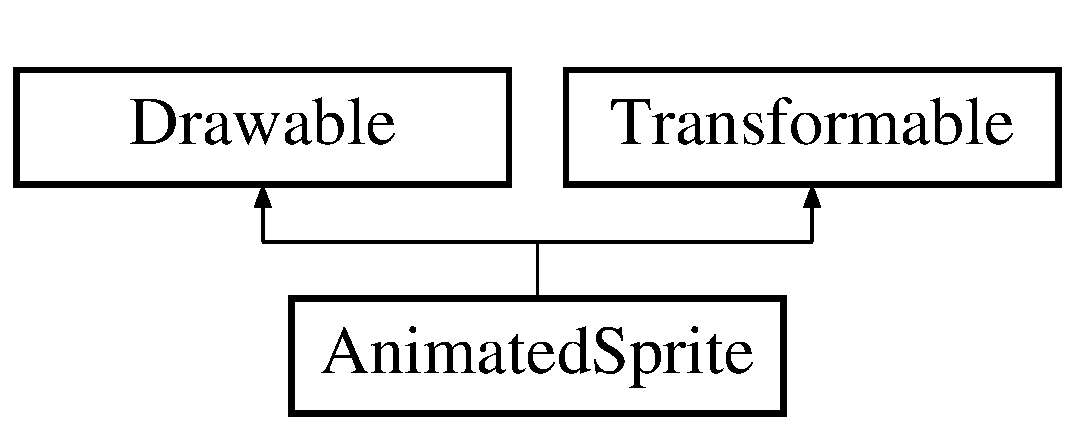
\includegraphics[height=2.000000cm]{classAnimatedSprite}
\end{center}
\end{figure}
\subsection*{Métodos públicos}
\begin{DoxyCompactItemize}
\item 
\hyperlink{classAnimatedSprite_a14c50aaf795c217f187f839d6cca9c76}{Animated\+Sprite} (sf\+::\+Time frame\+Time=sf\+::seconds(0.\+2f), bool paused=false, bool looped=true, bool wait=false)
\item 
void \hyperlink{classAnimatedSprite_a17a41ff812631a9d8947d272933d6696}{update} (sf\+::\+Time delta\+Time)
\item 
void \hyperlink{classAnimatedSprite_ab1afc57d90d57a0c4bc4f5b090f2dacf}{set\+Animation} (const \hyperlink{classAnimation}{Animation} \&animation)
\item 
void \hyperlink{classAnimatedSprite_af598fab5c3599ccc5ed1e2d4fefa68cc}{set\+Frame\+Time} (sf\+::\+Time time)
\item 
void \hyperlink{classAnimatedSprite_a203b968f1cb374cca5dbc89716174020}{play} ()
\item 
void \hyperlink{classAnimatedSprite_a9ea345649a4e012d096bc04aafe1ecb0}{play} (const \hyperlink{classAnimation}{Animation} \&animation)
\item 
void \hyperlink{classAnimatedSprite_a48384db59427423b5c1d98f6ee94fe45}{pause} ()
\item 
void \hyperlink{classAnimatedSprite_af9734f4346d3d2370322b2dcaeef133c}{stop} ()
\item 
void \hyperlink{classAnimatedSprite_af38c7271d7cd9af432952de2728f8fc9}{set\+Wait} (bool wait)
\item 
bool \hyperlink{classAnimatedSprite_a67698a0da51b5d4e008d1a9a33209603}{get\+Wait} ()
\item 
void \hyperlink{classAnimatedSprite_a855a5a48ea2e1c51c7c9304857dd2f8c}{set\+Looped} (bool looped)
\item 
void \hyperlink{classAnimatedSprite_a1a96a0f6570efddd2eb26f89bc5b6f50}{set\+Color} (const sf\+::\+Color \&color)
\item 
const \hyperlink{classAnimation}{Animation} $\ast$ \hyperlink{classAnimatedSprite_ad1f89db42fe276e8c8f603d5a501d1ed}{get\+Animation} () const 
\item 
\hypertarget{classAnimatedSprite_ab85f8836a5e03ba9b954243acd38556f}{}sf\+::\+Float\+Rect {\bfseries get\+Local\+Bounds} () const \label{classAnimatedSprite_ab85f8836a5e03ba9b954243acd38556f}

\item 
\hypertarget{classAnimatedSprite_a61f2bded199a5f39ae5d99cf110503a8}{}sf\+::\+Float\+Rect {\bfseries get\+Global\+Bounds} () const \label{classAnimatedSprite_a61f2bded199a5f39ae5d99cf110503a8}

\item 
bool \hyperlink{classAnimatedSprite_a9988efa6e5dc1868d27ec3345e0ffd11}{is\+Looped} () const 
\item 
bool \hyperlink{classAnimatedSprite_a07c49b95f177cedb4e8e82c709e1151c}{is\+Playing} () const 
\item 
sf\+::\+Time \hyperlink{classAnimatedSprite_ae36aaffc61eaed8848615f2394dba74f}{get\+Frame\+Time} () const 
\item 
void \hyperlink{classAnimatedSprite_a0b3e38fffdc1d29f46fa08df9ef2a747}{set\+Frame} (std\+::size\+\_\+t new\+Frame, bool reset\+Time=true)
\end{DoxyCompactItemize}


\subsection{Descripción detallada}
Clase para reproducir una animación 

\subsection{Documentación del constructor y destructor}
\hypertarget{classAnimatedSprite_a14c50aaf795c217f187f839d6cca9c76}{}\index{Animated\+Sprite@{Animated\+Sprite}!Animated\+Sprite@{Animated\+Sprite}}
\index{Animated\+Sprite@{Animated\+Sprite}!Animated\+Sprite@{Animated\+Sprite}}
\subsubsection[{Animated\+Sprite}]{\setlength{\rightskip}{0pt plus 5cm}Animated\+Sprite\+::\+Animated\+Sprite (
\begin{DoxyParamCaption}
\item[{sf\+::\+Time}]{frame\+Time = {\ttfamily sf\+:\+:seconds(0.2f)}, }
\item[{bool}]{paused = {\ttfamily false}, }
\item[{bool}]{looped = {\ttfamily true}, }
\item[{bool}]{wait = {\ttfamily false}}
\end{DoxyParamCaption}
)\hspace{0.3cm}{\ttfamily [explicit]}}\label{classAnimatedSprite_a14c50aaf795c217f187f839d6cca9c76}
Constructor 
\begin{DoxyParams}{Parámetros}
{\em frame\+Time} & tiempo entre frames de la animación \\
\hline
{\em paused} & por defecto false, establece si está pausado \\
\hline
{\em looped} & por defecto true, establece si es cíclico \\
\hline
{\em wait} & por defecto false, establece si hay que esperar a que la animación termine \\
\hline
\end{DoxyParams}


\subsection{Documentación de las funciones miembro}
\hypertarget{classAnimatedSprite_ad1f89db42fe276e8c8f603d5a501d1ed}{}\index{Animated\+Sprite@{Animated\+Sprite}!get\+Animation@{get\+Animation}}
\index{get\+Animation@{get\+Animation}!Animated\+Sprite@{Animated\+Sprite}}
\subsubsection[{get\+Animation}]{\setlength{\rightskip}{0pt plus 5cm}const {\bf Animation} $\ast$ Animated\+Sprite\+::get\+Animation (
\begin{DoxyParamCaption}
{}
\end{DoxyParamCaption}
) const}\label{classAnimatedSprite_ad1f89db42fe276e8c8f603d5a501d1ed}
Devuelve la animación \begin{DoxyReturn}{Devuelve}
la animación seteada 
\end{DoxyReturn}
\hypertarget{classAnimatedSprite_ae36aaffc61eaed8848615f2394dba74f}{}\index{Animated\+Sprite@{Animated\+Sprite}!get\+Frame\+Time@{get\+Frame\+Time}}
\index{get\+Frame\+Time@{get\+Frame\+Time}!Animated\+Sprite@{Animated\+Sprite}}
\subsubsection[{get\+Frame\+Time}]{\setlength{\rightskip}{0pt plus 5cm}sf\+::\+Time Animated\+Sprite\+::get\+Frame\+Time (
\begin{DoxyParamCaption}
{}
\end{DoxyParamCaption}
) const}\label{classAnimatedSprite_ae36aaffc61eaed8848615f2394dba74f}
Devuelve el tiempo entre frames de la animación \begin{DoxyReturn}{Devuelve}

\end{DoxyReturn}
\hypertarget{classAnimatedSprite_a67698a0da51b5d4e008d1a9a33209603}{}\index{Animated\+Sprite@{Animated\+Sprite}!get\+Wait@{get\+Wait}}
\index{get\+Wait@{get\+Wait}!Animated\+Sprite@{Animated\+Sprite}}
\subsubsection[{get\+Wait}]{\setlength{\rightskip}{0pt plus 5cm}bool Animated\+Sprite\+::get\+Wait (
\begin{DoxyParamCaption}
{}
\end{DoxyParamCaption}
)\hspace{0.3cm}{\ttfamily [inline]}}\label{classAnimatedSprite_a67698a0da51b5d4e008d1a9a33209603}
Devuelve si se espera por \begin{DoxyReturn}{Devuelve}

\end{DoxyReturn}
\hypertarget{classAnimatedSprite_a9988efa6e5dc1868d27ec3345e0ffd11}{}\index{Animated\+Sprite@{Animated\+Sprite}!is\+Looped@{is\+Looped}}
\index{is\+Looped@{is\+Looped}!Animated\+Sprite@{Animated\+Sprite}}
\subsubsection[{is\+Looped}]{\setlength{\rightskip}{0pt plus 5cm}bool Animated\+Sprite\+::is\+Looped (
\begin{DoxyParamCaption}
{}
\end{DoxyParamCaption}
) const}\label{classAnimatedSprite_a9988efa6e5dc1868d27ec3345e0ffd11}
Indica si es cíclico \begin{DoxyReturn}{Devuelve}

\end{DoxyReturn}
\hypertarget{classAnimatedSprite_a07c49b95f177cedb4e8e82c709e1151c}{}\index{Animated\+Sprite@{Animated\+Sprite}!is\+Playing@{is\+Playing}}
\index{is\+Playing@{is\+Playing}!Animated\+Sprite@{Animated\+Sprite}}
\subsubsection[{is\+Playing}]{\setlength{\rightskip}{0pt plus 5cm}bool Animated\+Sprite\+::is\+Playing (
\begin{DoxyParamCaption}
{}
\end{DoxyParamCaption}
) const}\label{classAnimatedSprite_a07c49b95f177cedb4e8e82c709e1151c}
Indica si se está reproduciendo \begin{DoxyReturn}{Devuelve}

\end{DoxyReturn}
\hypertarget{classAnimatedSprite_a48384db59427423b5c1d98f6ee94fe45}{}\index{Animated\+Sprite@{Animated\+Sprite}!pause@{pause}}
\index{pause@{pause}!Animated\+Sprite@{Animated\+Sprite}}
\subsubsection[{pause}]{\setlength{\rightskip}{0pt plus 5cm}void Animated\+Sprite\+::pause (
\begin{DoxyParamCaption}
{}
\end{DoxyParamCaption}
)}\label{classAnimatedSprite_a48384db59427423b5c1d98f6ee94fe45}
Pausa la animación \hypertarget{classAnimatedSprite_a203b968f1cb374cca5dbc89716174020}{}\index{Animated\+Sprite@{Animated\+Sprite}!play@{play}}
\index{play@{play}!Animated\+Sprite@{Animated\+Sprite}}
\subsubsection[{play}]{\setlength{\rightskip}{0pt plus 5cm}void Animated\+Sprite\+::play (
\begin{DoxyParamCaption}
{}
\end{DoxyParamCaption}
)}\label{classAnimatedSprite_a203b968f1cb374cca5dbc89716174020}
Reproduce la animación \hypertarget{classAnimatedSprite_a9ea345649a4e012d096bc04aafe1ecb0}{}\index{Animated\+Sprite@{Animated\+Sprite}!play@{play}}
\index{play@{play}!Animated\+Sprite@{Animated\+Sprite}}
\subsubsection[{play}]{\setlength{\rightskip}{0pt plus 5cm}void Animated\+Sprite\+::play (
\begin{DoxyParamCaption}
\item[{const {\bf Animation} \&}]{animation}
\end{DoxyParamCaption}
)}\label{classAnimatedSprite_a9ea345649a4e012d096bc04aafe1ecb0}
Reproduce la animación dada y la setea 
\begin{DoxyParams}{Parámetros}
{\em animation} & \\
\hline
\end{DoxyParams}
\hypertarget{classAnimatedSprite_ab1afc57d90d57a0c4bc4f5b090f2dacf}{}\index{Animated\+Sprite@{Animated\+Sprite}!set\+Animation@{set\+Animation}}
\index{set\+Animation@{set\+Animation}!Animated\+Sprite@{Animated\+Sprite}}
\subsubsection[{set\+Animation}]{\setlength{\rightskip}{0pt plus 5cm}void Animated\+Sprite\+::set\+Animation (
\begin{DoxyParamCaption}
\item[{const {\bf Animation} \&}]{animation}
\end{DoxyParamCaption}
)}\label{classAnimatedSprite_ab1afc57d90d57a0c4bc4f5b090f2dacf}
Establece la animación 
\begin{DoxyParams}{Parámetros}
{\em animation} & animación a setear \\
\hline
\end{DoxyParams}
\hypertarget{classAnimatedSprite_a1a96a0f6570efddd2eb26f89bc5b6f50}{}\index{Animated\+Sprite@{Animated\+Sprite}!set\+Color@{set\+Color}}
\index{set\+Color@{set\+Color}!Animated\+Sprite@{Animated\+Sprite}}
\subsubsection[{set\+Color}]{\setlength{\rightskip}{0pt plus 5cm}void Animated\+Sprite\+::set\+Color (
\begin{DoxyParamCaption}
\item[{const sf\+::\+Color \&}]{color}
\end{DoxyParamCaption}
)}\label{classAnimatedSprite_a1a96a0f6570efddd2eb26f89bc5b6f50}
C\+Olorea los vértices 
\begin{DoxyParams}{Parámetros}
{\em color} & \\
\hline
\end{DoxyParams}
\hypertarget{classAnimatedSprite_a0b3e38fffdc1d29f46fa08df9ef2a747}{}\index{Animated\+Sprite@{Animated\+Sprite}!set\+Frame@{set\+Frame}}
\index{set\+Frame@{set\+Frame}!Animated\+Sprite@{Animated\+Sprite}}
\subsubsection[{set\+Frame}]{\setlength{\rightskip}{0pt plus 5cm}void Animated\+Sprite\+::set\+Frame (
\begin{DoxyParamCaption}
\item[{std\+::size\+\_\+t}]{new\+Frame, }
\item[{bool}]{reset\+Time = {\ttfamily true}}
\end{DoxyParamCaption}
)}\label{classAnimatedSprite_a0b3e38fffdc1d29f46fa08df9ef2a747}
Setea el frame indicado 
\begin{DoxyParams}{Parámetros}
{\em new\+Frame} & el indice del frame a setear \\
\hline
{\em reset\+Time} & por defecto true, si se empieza a contar desde cero el tiempo de frame \\
\hline
\end{DoxyParams}
\hypertarget{classAnimatedSprite_af598fab5c3599ccc5ed1e2d4fefa68cc}{}\index{Animated\+Sprite@{Animated\+Sprite}!set\+Frame\+Time@{set\+Frame\+Time}}
\index{set\+Frame\+Time@{set\+Frame\+Time}!Animated\+Sprite@{Animated\+Sprite}}
\subsubsection[{set\+Frame\+Time}]{\setlength{\rightskip}{0pt plus 5cm}void Animated\+Sprite\+::set\+Frame\+Time (
\begin{DoxyParamCaption}
\item[{sf\+::\+Time}]{time}
\end{DoxyParamCaption}
)}\label{classAnimatedSprite_af598fab5c3599ccc5ed1e2d4fefa68cc}
Establece el tiempo entre los frames de la animación 
\begin{DoxyParams}{Parámetros}
{\em time} & \\
\hline
\end{DoxyParams}
\hypertarget{classAnimatedSprite_a855a5a48ea2e1c51c7c9304857dd2f8c}{}\index{Animated\+Sprite@{Animated\+Sprite}!set\+Looped@{set\+Looped}}
\index{set\+Looped@{set\+Looped}!Animated\+Sprite@{Animated\+Sprite}}
\subsubsection[{set\+Looped}]{\setlength{\rightskip}{0pt plus 5cm}void Animated\+Sprite\+::set\+Looped (
\begin{DoxyParamCaption}
\item[{bool}]{looped}
\end{DoxyParamCaption}
)}\label{classAnimatedSprite_a855a5a48ea2e1c51c7c9304857dd2f8c}
Setea si es cíclico 
\begin{DoxyParams}{Parámetros}
{\em looped} & true si es cíclico \\
\hline
\end{DoxyParams}
\hypertarget{classAnimatedSprite_af38c7271d7cd9af432952de2728f8fc9}{}\index{Animated\+Sprite@{Animated\+Sprite}!set\+Wait@{set\+Wait}}
\index{set\+Wait@{set\+Wait}!Animated\+Sprite@{Animated\+Sprite}}
\subsubsection[{set\+Wait}]{\setlength{\rightskip}{0pt plus 5cm}void Animated\+Sprite\+::set\+Wait (
\begin{DoxyParamCaption}
\item[{bool}]{wait}
\end{DoxyParamCaption}
)\hspace{0.3cm}{\ttfamily [inline]}}\label{classAnimatedSprite_af38c7271d7cd9af432952de2728f8fc9}
Setea si se espera al final de la animación 
\begin{DoxyParams}{Parámetros}
{\em wait} & true si se espera, false al contrario \\
\hline
\end{DoxyParams}
\hypertarget{classAnimatedSprite_af9734f4346d3d2370322b2dcaeef133c}{}\index{Animated\+Sprite@{Animated\+Sprite}!stop@{stop}}
\index{stop@{stop}!Animated\+Sprite@{Animated\+Sprite}}
\subsubsection[{stop}]{\setlength{\rightskip}{0pt plus 5cm}void Animated\+Sprite\+::stop (
\begin{DoxyParamCaption}
{}
\end{DoxyParamCaption}
)}\label{classAnimatedSprite_af9734f4346d3d2370322b2dcaeef133c}
Para la animación \hypertarget{classAnimatedSprite_a17a41ff812631a9d8947d272933d6696}{}\index{Animated\+Sprite@{Animated\+Sprite}!update@{update}}
\index{update@{update}!Animated\+Sprite@{Animated\+Sprite}}
\subsubsection[{update}]{\setlength{\rightskip}{0pt plus 5cm}void Animated\+Sprite\+::update (
\begin{DoxyParamCaption}
\item[{sf\+::\+Time}]{delta\+Time}
\end{DoxyParamCaption}
)}\label{classAnimatedSprite_a17a41ff812631a9d8947d272933d6696}
Actualiza la animación 
\begin{DoxyParams}{Parámetros}
{\em delta\+Time} & tiempo entre frame y frame \\
\hline
\end{DoxyParams}


La documentación para esta clase fue generada a partir de los siguientes ficheros\+:\begin{DoxyCompactItemize}
\item 
Animated\+Sprite.\+h\item 
Animated\+Sprite.\+cpp\end{DoxyCompactItemize}

\hypertarget{classAnimation}{}\section{Referencia de la Clase Animation}
\label{classAnimation}\index{Animation@{Animation}}


{\ttfamily \#include $<$Animation.\+h$>$}

\subsection*{Métodos públicos}
\begin{DoxyCompactItemize}
\item 
\hyperlink{classAnimation_a83f0a16cef7117f187ad596de38dd9d6}{Animation} ()
\item 
void \hyperlink{classAnimation_a486ee5fa2d40ae90f227a19866998c91}{add\+Frame} (sf\+::\+Int\+Rect rect)
\item 
void \hyperlink{classAnimation_a2fb16f452a323d51a0104c0aa454cab3}{set\+Sprite\+Sheet} (const sf\+::\+Texture \&texture)
\item 
const sf\+::\+Texture $\ast$ \hyperlink{classAnimation_aafed5696c35b893bb721aa1303d5e84f}{get\+Sprite\+Sheet} () const 
\item 
std\+::size\+\_\+t \hyperlink{classAnimation_aa8dc627c1800fcad9b9e53c9a102ded3}{get\+Size} () const 
\item 
const sf\+::\+Int\+Rect \& \hyperlink{classAnimation_ad587678b331518e926b19b807b153daa}{get\+Frame} (std\+::size\+\_\+t n) const 
\item 
void \hyperlink{classAnimation_ae12f4c253d6c83ee8407a5395a270f6e}{set\+Replay} (bool replay)
\item 
bool \hyperlink{classAnimation_a553400098a1be7345942f1c189b5d78d}{get\+Replay} ()
\item 
void \hyperlink{classAnimation_a17273537e876ed1f04857601fb484091}{set\+Wait} (bool wait)
\item 
bool \hyperlink{classAnimation_ab0f6daf2ca2965d75e6ab480025de553}{get\+Wait} ()
\end{DoxyCompactItemize}


\subsection{Descripción detallada}
Clase para las animaciones, guarda la lista de frames de una animación concreta 

\subsection{Documentación del constructor y destructor}
\hypertarget{classAnimation_a83f0a16cef7117f187ad596de38dd9d6}{}\index{Animation@{Animation}!Animation@{Animation}}
\index{Animation@{Animation}!Animation@{Animation}}
\subsubsection[{Animation}]{\setlength{\rightskip}{0pt plus 5cm}Animation\+::\+Animation (
\begin{DoxyParamCaption}
{}
\end{DoxyParamCaption}
)}\label{classAnimation_a83f0a16cef7117f187ad596de38dd9d6}
Constructor 

\subsection{Documentación de las funciones miembro}
\hypertarget{classAnimation_a486ee5fa2d40ae90f227a19866998c91}{}\index{Animation@{Animation}!add\+Frame@{add\+Frame}}
\index{add\+Frame@{add\+Frame}!Animation@{Animation}}
\subsubsection[{add\+Frame}]{\setlength{\rightskip}{0pt plus 5cm}void Animation\+::add\+Frame (
\begin{DoxyParamCaption}
\item[{sf\+::\+Int\+Rect}]{rect}
\end{DoxyParamCaption}
)}\label{classAnimation_a486ee5fa2d40ae90f227a19866998c91}
Añade un frame 
\begin{DoxyParams}{Parámetros}
{\em rect} & rectángulo que define el frame en la imagen \\
\hline
\end{DoxyParams}
\hypertarget{classAnimation_ad587678b331518e926b19b807b153daa}{}\index{Animation@{Animation}!get\+Frame@{get\+Frame}}
\index{get\+Frame@{get\+Frame}!Animation@{Animation}}
\subsubsection[{get\+Frame}]{\setlength{\rightskip}{0pt plus 5cm}const sf\+::\+Int\+Rect \& Animation\+::get\+Frame (
\begin{DoxyParamCaption}
\item[{std\+::size\+\_\+t}]{n}
\end{DoxyParamCaption}
) const}\label{classAnimation_ad587678b331518e926b19b807b153daa}
Devuelve el rectángulo del frame especificado 
\begin{DoxyParams}{Parámetros}
{\em n} & numero de frame \\
\hline
\end{DoxyParams}
\begin{DoxyReturn}{Devuelve}
rectangulo del frame 
\end{DoxyReturn}
\hypertarget{classAnimation_a553400098a1be7345942f1c189b5d78d}{}\index{Animation@{Animation}!get\+Replay@{get\+Replay}}
\index{get\+Replay@{get\+Replay}!Animation@{Animation}}
\subsubsection[{get\+Replay}]{\setlength{\rightskip}{0pt plus 5cm}bool Animation\+::get\+Replay (
\begin{DoxyParamCaption}
{}
\end{DoxyParamCaption}
)\hspace{0.3cm}{\ttfamily [inline]}}\label{classAnimation_a553400098a1be7345942f1c189b5d78d}
Devuelve si la animación es cíclica \begin{DoxyReturn}{Devuelve}
true si es cíclica 
\end{DoxyReturn}
\hypertarget{classAnimation_aa8dc627c1800fcad9b9e53c9a102ded3}{}\index{Animation@{Animation}!get\+Size@{get\+Size}}
\index{get\+Size@{get\+Size}!Animation@{Animation}}
\subsubsection[{get\+Size}]{\setlength{\rightskip}{0pt plus 5cm}std\+::size\+\_\+t Animation\+::get\+Size (
\begin{DoxyParamCaption}
{}
\end{DoxyParamCaption}
) const}\label{classAnimation_aa8dc627c1800fcad9b9e53c9a102ded3}
Devuelve el número de frames \begin{DoxyReturn}{Devuelve}
numero de frames 
\end{DoxyReturn}
\hypertarget{classAnimation_aafed5696c35b893bb721aa1303d5e84f}{}\index{Animation@{Animation}!get\+Sprite\+Sheet@{get\+Sprite\+Sheet}}
\index{get\+Sprite\+Sheet@{get\+Sprite\+Sheet}!Animation@{Animation}}
\subsubsection[{get\+Sprite\+Sheet}]{\setlength{\rightskip}{0pt plus 5cm}const sf\+::\+Texture $\ast$ Animation\+::get\+Sprite\+Sheet (
\begin{DoxyParamCaption}
{}
\end{DoxyParamCaption}
) const}\label{classAnimation_aafed5696c35b893bb721aa1303d5e84f}
Devuelve la imagen donde estan los frames \begin{DoxyReturn}{Devuelve}
imagen 
\end{DoxyReturn}
\hypertarget{classAnimation_ab0f6daf2ca2965d75e6ab480025de553}{}\index{Animation@{Animation}!get\+Wait@{get\+Wait}}
\index{get\+Wait@{get\+Wait}!Animation@{Animation}}
\subsubsection[{get\+Wait}]{\setlength{\rightskip}{0pt plus 5cm}bool Animation\+::get\+Wait (
\begin{DoxyParamCaption}
{}
\end{DoxyParamCaption}
)\hspace{0.3cm}{\ttfamily [inline]}}\label{classAnimation_ab0f6daf2ca2965d75e6ab480025de553}
Indica si hay que esperar a que la animación finalice \begin{DoxyReturn}{Devuelve}
true si hay que esperar a que finalice la animación 
\end{DoxyReturn}
\hypertarget{classAnimation_ae12f4c253d6c83ee8407a5395a270f6e}{}\index{Animation@{Animation}!set\+Replay@{set\+Replay}}
\index{set\+Replay@{set\+Replay}!Animation@{Animation}}
\subsubsection[{set\+Replay}]{\setlength{\rightskip}{0pt plus 5cm}void Animation\+::set\+Replay (
\begin{DoxyParamCaption}
\item[{bool}]{replay}
\end{DoxyParamCaption}
)\hspace{0.3cm}{\ttfamily [inline]}}\label{classAnimation_ae12f4c253d6c83ee8407a5395a270f6e}
Establece si la animación es cíclica 
\begin{DoxyParams}{Parámetros}
{\em replay} & true si es cíclica \\
\hline
\end{DoxyParams}
\hypertarget{classAnimation_a2fb16f452a323d51a0104c0aa454cab3}{}\index{Animation@{Animation}!set\+Sprite\+Sheet@{set\+Sprite\+Sheet}}
\index{set\+Sprite\+Sheet@{set\+Sprite\+Sheet}!Animation@{Animation}}
\subsubsection[{set\+Sprite\+Sheet}]{\setlength{\rightskip}{0pt plus 5cm}void Animation\+::set\+Sprite\+Sheet (
\begin{DoxyParamCaption}
\item[{const sf\+::\+Texture \&}]{texture}
\end{DoxyParamCaption}
)}\label{classAnimation_a2fb16f452a323d51a0104c0aa454cab3}
Estblece la imagen donde estan los frames 
\begin{DoxyParams}{Parámetros}
{\em texture} & imagen \\
\hline
\end{DoxyParams}
\hypertarget{classAnimation_a17273537e876ed1f04857601fb484091}{}\index{Animation@{Animation}!set\+Wait@{set\+Wait}}
\index{set\+Wait@{set\+Wait}!Animation@{Animation}}
\subsubsection[{set\+Wait}]{\setlength{\rightskip}{0pt plus 5cm}void Animation\+::set\+Wait (
\begin{DoxyParamCaption}
\item[{bool}]{wait}
\end{DoxyParamCaption}
)\hspace{0.3cm}{\ttfamily [inline]}}\label{classAnimation_a17273537e876ed1f04857601fb484091}
Establece si hay que esperar a que la animación finalice 
\begin{DoxyParams}{Parámetros}
{\em wait} & true si hay que esperar a que finalice la animación \\
\hline
\end{DoxyParams}


La documentación para esta clase fue generada a partir de los siguientes ficheros\+:\begin{DoxyCompactItemize}
\item 
Animation.\+h\item 
Animation.\+cpp\end{DoxyCompactItemize}

\hypertarget{classApplication}{}\section{Referencia de la Clase Application}
\label{classApplication}\index{Application@{Application}}
\subsection*{Métodos públicos}
\begin{DoxyCompactItemize}
\item 
\hyperlink{classApplication_afa8cc05ce6b6092be5ecdfdae44e05f8}{Application} ()
\item 
void \hyperlink{classApplication_a68965449404743bf1add056784d6cf81}{run} ()
\end{DoxyCompactItemize}


\subsection{Documentación del constructor y destructor}
\hypertarget{classApplication_afa8cc05ce6b6092be5ecdfdae44e05f8}{}\index{Application@{Application}!Application@{Application}}
\index{Application@{Application}!Application@{Application}}
\subsubsection[{Application}]{\setlength{\rightskip}{0pt plus 5cm}Application\+::\+Application (
\begin{DoxyParamCaption}
{}
\end{DoxyParamCaption}
)}\label{classApplication_afa8cc05ce6b6092be5ecdfdae44e05f8}
Constructor 

\subsection{Documentación de las funciones miembro}
\hypertarget{classApplication_a68965449404743bf1add056784d6cf81}{}\index{Application@{Application}!run@{run}}
\index{run@{run}!Application@{Application}}
\subsubsection[{run}]{\setlength{\rightskip}{0pt plus 5cm}void Application\+::run (
\begin{DoxyParamCaption}
{}
\end{DoxyParamCaption}
)}\label{classApplication_a68965449404743bf1add056784d6cf81}
Inicializa la aplicación 

La documentación para esta clase fue generada a partir de los siguientes ficheros\+:\begin{DoxyCompactItemize}
\item 
Application.\+h\item 
Application.\+cpp\end{DoxyCompactItemize}

\hypertarget{structBehaviour}{}\section{Referencia de la Estructura Behaviour}
\label{structBehaviour}\index{Behaviour@{Behaviour}}


{\ttfamily \#include $<$Behaviour.\+h$>$}

\subsection*{Campos de datos}
\begin{DoxyCompactItemize}
\item 
std\+::function$<$ void(Actions action, \hyperlink{classPropertyManager}{Property\+Manager} $\ast$prop)$>$ \hyperlink{structBehaviour_a870609da80d44c4825b2de567e28dd24}{behaviour\+Function}
\end{DoxyCompactItemize}


\subsection{Descripción detallada}
Estructura de comportamiento que guarda una función a ejecutar 

\subsection{Documentación de los campos}
\hypertarget{structBehaviour_a870609da80d44c4825b2de567e28dd24}{}\index{Behaviour@{Behaviour}!behaviour\+Function@{behaviour\+Function}}
\index{behaviour\+Function@{behaviour\+Function}!Behaviour@{Behaviour}}
\subsubsection[{behaviour\+Function}]{\setlength{\rightskip}{0pt plus 5cm}std\+::function$<$void(Actions action, {\bf Property\+Manager}$\ast$ prop)$>$ Behaviour\+::behaviour\+Function}\label{structBehaviour_a870609da80d44c4825b2de567e28dd24}
Guarda una función que especifica la acción realizada y una serie de propiedades 

La documentación para esta estructura fue generada a partir del siguiente fichero\+:\begin{DoxyCompactItemize}
\item 
Behaviour.\+h\end{DoxyCompactItemize}

\hypertarget{classGUI_1_1Button}{}\section{Referencia de la Clase G\+U\+I\+:\+:Button}
\label{classGUI_1_1Button}\index{G\+U\+I\+::\+Button@{G\+U\+I\+::\+Button}}


{\ttfamily \#include $<$Button.\+h$>$}

Diagrama de herencias de G\+U\+I\+:\+:Button\begin{figure}[H]
\begin{center}
\leavevmode
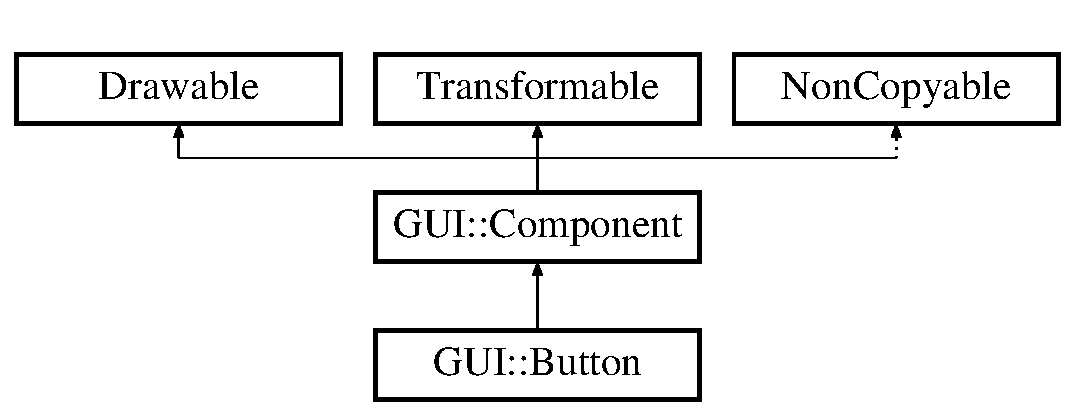
\includegraphics[height=3.000000cm]{classGUI_1_1Button}
\end{center}
\end{figure}
\subsection*{Tipos públicos}
\begin{DoxyCompactItemize}
\item 
typedef std\+::function$<$ void() $>$ \hyperlink{classGUI_1_1Button_ae42ce66ac9fd4834cef81bb6f2fb0dab}{Callback}
\end{DoxyCompactItemize}
\subsection*{Métodos públicos}
\begin{DoxyCompactItemize}
\item 
\hyperlink{classGUI_1_1Button_a3e3c8c068b07a9865b516560f93cb253}{Button} (\hyperlink{classContext}{Context} context)
\item 
virtual \hyperlink{classGUI_1_1Button_a98edcfb20ac836db54ecda4260eac1d9}{$\sim$\+Button} ()
\item 
void \hyperlink{classGUI_1_1Button_ae5ac54c7429eaa482eb7069d0efdb79f}{set\+Callback} (\hyperlink{classGUI_1_1Button_ae42ce66ac9fd4834cef81bb6f2fb0dab}{Callback} callback)
\item 
void \hyperlink{classGUI_1_1Button_a26ddad6fdc253dbbc593f0204c15fb24}{set\+Text} (const wchar\+\_\+t $\ast$text)
\item 
void \hyperlink{classGUI_1_1Button_a8198052cf4fe5823c9f5513e778ca94d}{set\+Toggle} (bool flag)
\item 
virtual bool \hyperlink{classGUI_1_1Button_a2fba8dea2886fd3bb33c7e250e695e8a}{is\+Selectable} () const 
\item 
virtual void \hyperlink{classGUI_1_1Button_a8f141129acb9c068ba6b8d19974d8291}{select} ()
\item 
virtual void \hyperlink{classGUI_1_1Button_a6fd040a471dc3ae48ad59cacd93c7292}{deselect} ()
\item 
virtual void \hyperlink{classGUI_1_1Button_ad711a129863e0301c52b896911996123}{activate} ()
\item 
virtual void \hyperlink{classGUI_1_1Button_ab0a1773817447712b17ab1ad6da767da}{deactivate} ()
\item 
virtual void \hyperlink{classGUI_1_1Button_a4d30e4caedd4c4373567ef452acd1fb1}{handle\+Event} (const sf\+::\+Event \&event)
\end{DoxyCompactItemize}


\subsection{Descripción detallada}
Representa un botón en la G\+U\+I 

\subsection{Documentación de los \textquotesingle{}Typedef\textquotesingle{} miembros de la clase}
\hypertarget{classGUI_1_1Button_ae42ce66ac9fd4834cef81bb6f2fb0dab}{}\index{G\+U\+I\+::\+Button@{G\+U\+I\+::\+Button}!Callback@{Callback}}
\index{Callback@{Callback}!G\+U\+I\+::\+Button@{G\+U\+I\+::\+Button}}
\subsubsection[{Callback}]{\setlength{\rightskip}{0pt plus 5cm}typedef std\+::function$<$void() $>$ {\bf G\+U\+I\+::\+Button\+::\+Callback}}\label{classGUI_1_1Button_ae42ce66ac9fd4834cef81bb6f2fb0dab}
Define un alias para guardar una función 

\subsection{Documentación del constructor y destructor}
\hypertarget{classGUI_1_1Button_a3e3c8c068b07a9865b516560f93cb253}{}\index{G\+U\+I\+::\+Button@{G\+U\+I\+::\+Button}!Button@{Button}}
\index{Button@{Button}!G\+U\+I\+::\+Button@{G\+U\+I\+::\+Button}}
\subsubsection[{Button}]{\setlength{\rightskip}{0pt plus 5cm}G\+U\+I\+::\+Button\+::\+Button (
\begin{DoxyParamCaption}
\item[{{\bf Context}}]{context}
\end{DoxyParamCaption}
)}\label{classGUI_1_1Button_a3e3c8c068b07a9865b516560f93cb253}
Constructor 
\begin{DoxyParams}{Parámetros}
{\em context} & contexto de la aplicación \\
\hline
\end{DoxyParams}
\hypertarget{classGUI_1_1Button_a98edcfb20ac836db54ecda4260eac1d9}{}\index{G\+U\+I\+::\+Button@{G\+U\+I\+::\+Button}!````~Button@{$\sim$\+Button}}
\index{````~Button@{$\sim$\+Button}!G\+U\+I\+::\+Button@{G\+U\+I\+::\+Button}}
\subsubsection[{$\sim$\+Button}]{\setlength{\rightskip}{0pt plus 5cm}G\+U\+I\+::\+Button\+::$\sim$\+Button (
\begin{DoxyParamCaption}
{}
\end{DoxyParamCaption}
)\hspace{0.3cm}{\ttfamily [virtual]}}\label{classGUI_1_1Button_a98edcfb20ac836db54ecda4260eac1d9}
Destructor 

\subsection{Documentación de las funciones miembro}
\hypertarget{classGUI_1_1Button_ad711a129863e0301c52b896911996123}{}\index{G\+U\+I\+::\+Button@{G\+U\+I\+::\+Button}!activate@{activate}}
\index{activate@{activate}!G\+U\+I\+::\+Button@{G\+U\+I\+::\+Button}}
\subsubsection[{activate}]{\setlength{\rightskip}{0pt plus 5cm}void G\+U\+I\+::\+Button\+::activate (
\begin{DoxyParamCaption}
{}
\end{DoxyParamCaption}
)\hspace{0.3cm}{\ttfamily [virtual]}}\label{classGUI_1_1Button_ad711a129863e0301c52b896911996123}
Activa el componente 

Reimplementado de \hyperlink{classGUI_1_1Component_a965823e0e62612a7e532eb8c0b98861d}{G\+U\+I\+::\+Component}.

\hypertarget{classGUI_1_1Button_ab0a1773817447712b17ab1ad6da767da}{}\index{G\+U\+I\+::\+Button@{G\+U\+I\+::\+Button}!deactivate@{deactivate}}
\index{deactivate@{deactivate}!G\+U\+I\+::\+Button@{G\+U\+I\+::\+Button}}
\subsubsection[{deactivate}]{\setlength{\rightskip}{0pt plus 5cm}void G\+U\+I\+::\+Button\+::deactivate (
\begin{DoxyParamCaption}
{}
\end{DoxyParamCaption}
)\hspace{0.3cm}{\ttfamily [virtual]}}\label{classGUI_1_1Button_ab0a1773817447712b17ab1ad6da767da}
Desactiva el componente 

Reimplementado de \hyperlink{classGUI_1_1Component_a8964087afef859c015fb8188e619aa81}{G\+U\+I\+::\+Component}.

\hypertarget{classGUI_1_1Button_a6fd040a471dc3ae48ad59cacd93c7292}{}\index{G\+U\+I\+::\+Button@{G\+U\+I\+::\+Button}!deselect@{deselect}}
\index{deselect@{deselect}!G\+U\+I\+::\+Button@{G\+U\+I\+::\+Button}}
\subsubsection[{deselect}]{\setlength{\rightskip}{0pt plus 5cm}void G\+U\+I\+::\+Button\+::deselect (
\begin{DoxyParamCaption}
{}
\end{DoxyParamCaption}
)\hspace{0.3cm}{\ttfamily [virtual]}}\label{classGUI_1_1Button_a6fd040a471dc3ae48ad59cacd93c7292}
Deselecciona el componente 

Reimplementado de \hyperlink{classGUI_1_1Component_aa37424b238293bb308d357cf3b35c81f}{G\+U\+I\+::\+Component}.

\hypertarget{classGUI_1_1Button_a4d30e4caedd4c4373567ef452acd1fb1}{}\index{G\+U\+I\+::\+Button@{G\+U\+I\+::\+Button}!handle\+Event@{handle\+Event}}
\index{handle\+Event@{handle\+Event}!G\+U\+I\+::\+Button@{G\+U\+I\+::\+Button}}
\subsubsection[{handle\+Event}]{\setlength{\rightskip}{0pt plus 5cm}void G\+U\+I\+::\+Button\+::handle\+Event (
\begin{DoxyParamCaption}
\item[{const sf\+::\+Event \&}]{event}
\end{DoxyParamCaption}
)\hspace{0.3cm}{\ttfamily [virtual]}}\label{classGUI_1_1Button_a4d30e4caedd4c4373567ef452acd1fb1}
Maneja los eventos capturados 
\begin{DoxyParams}{Parámetros}
{\em event} & evento capturado \\
\hline
\end{DoxyParams}


Implementa \hyperlink{classGUI_1_1Component_aacf5e981e7b5726f5c7e9436455660ba}{G\+U\+I\+::\+Component}.

\hypertarget{classGUI_1_1Button_a2fba8dea2886fd3bb33c7e250e695e8a}{}\index{G\+U\+I\+::\+Button@{G\+U\+I\+::\+Button}!is\+Selectable@{is\+Selectable}}
\index{is\+Selectable@{is\+Selectable}!G\+U\+I\+::\+Button@{G\+U\+I\+::\+Button}}
\subsubsection[{is\+Selectable}]{\setlength{\rightskip}{0pt plus 5cm}bool G\+U\+I\+::\+Button\+::is\+Selectable (
\begin{DoxyParamCaption}
{}
\end{DoxyParamCaption}
) const\hspace{0.3cm}{\ttfamily [virtual]}}\label{classGUI_1_1Button_a2fba8dea2886fd3bb33c7e250e695e8a}
Devuelve si el componente es seleccionable \begin{DoxyReturn}{Devuelve}
true si es seleccionable 
\end{DoxyReturn}


Implementa \hyperlink{classGUI_1_1Component_a44d14506c9a1dbc839e05a6bf99c341b}{G\+U\+I\+::\+Component}.

\hypertarget{classGUI_1_1Button_a8f141129acb9c068ba6b8d19974d8291}{}\index{G\+U\+I\+::\+Button@{G\+U\+I\+::\+Button}!select@{select}}
\index{select@{select}!G\+U\+I\+::\+Button@{G\+U\+I\+::\+Button}}
\subsubsection[{select}]{\setlength{\rightskip}{0pt plus 5cm}void G\+U\+I\+::\+Button\+::select (
\begin{DoxyParamCaption}
{}
\end{DoxyParamCaption}
)\hspace{0.3cm}{\ttfamily [virtual]}}\label{classGUI_1_1Button_a8f141129acb9c068ba6b8d19974d8291}
Selecciona el componente 

Reimplementado de \hyperlink{classGUI_1_1Component_ad0f7d6cc692edf2b0e426bfbd584be45}{G\+U\+I\+::\+Component}.

\hypertarget{classGUI_1_1Button_ae5ac54c7429eaa482eb7069d0efdb79f}{}\index{G\+U\+I\+::\+Button@{G\+U\+I\+::\+Button}!set\+Callback@{set\+Callback}}
\index{set\+Callback@{set\+Callback}!G\+U\+I\+::\+Button@{G\+U\+I\+::\+Button}}
\subsubsection[{set\+Callback}]{\setlength{\rightskip}{0pt plus 5cm}void G\+U\+I\+::\+Button\+::set\+Callback (
\begin{DoxyParamCaption}
\item[{{\bf Callback}}]{callback}
\end{DoxyParamCaption}
)}\label{classGUI_1_1Button_ae5ac54c7429eaa482eb7069d0efdb79f}
Establece la función que se ejecutará con el botón 
\begin{DoxyParams}{Parámetros}
{\em callback} & función \\
\hline
\end{DoxyParams}
\hypertarget{classGUI_1_1Button_a26ddad6fdc253dbbc593f0204c15fb24}{}\index{G\+U\+I\+::\+Button@{G\+U\+I\+::\+Button}!set\+Text@{set\+Text}}
\index{set\+Text@{set\+Text}!G\+U\+I\+::\+Button@{G\+U\+I\+::\+Button}}
\subsubsection[{set\+Text}]{\setlength{\rightskip}{0pt plus 5cm}void G\+U\+I\+::\+Button\+::set\+Text (
\begin{DoxyParamCaption}
\item[{const wchar\+\_\+t $\ast$}]{text}
\end{DoxyParamCaption}
)}\label{classGUI_1_1Button_a26ddad6fdc253dbbc593f0204c15fb24}
Setea el texto del botón 
\begin{DoxyParams}{Parámetros}
{\em text} & texto \\
\hline
\end{DoxyParams}
\hypertarget{classGUI_1_1Button_a8198052cf4fe5823c9f5513e778ca94d}{}\index{G\+U\+I\+::\+Button@{G\+U\+I\+::\+Button}!set\+Toggle@{set\+Toggle}}
\index{set\+Toggle@{set\+Toggle}!G\+U\+I\+::\+Button@{G\+U\+I\+::\+Button}}
\subsubsection[{set\+Toggle}]{\setlength{\rightskip}{0pt plus 5cm}void G\+U\+I\+::\+Button\+::set\+Toggle (
\begin{DoxyParamCaption}
\item[{bool}]{flag}
\end{DoxyParamCaption}
)}\label{classGUI_1_1Button_a8198052cf4fe5823c9f5513e778ca94d}
Establece si tendrá dos estados o solo uno 
\begin{DoxyParams}{Parámetros}
{\em flag} & true si tendrá dos estados \\
\hline
\end{DoxyParams}


La documentación para esta clase fue generada a partir de los siguientes ficheros\+:\begin{DoxyCompactItemize}
\item 
Button.\+h\item 
Button.\+cpp\end{DoxyCompactItemize}

\hypertarget{classChangeLevel}{}\section{Referencia de la Clase Change\+Level}
\label{classChangeLevel}\index{Change\+Level@{Change\+Level}}


{\ttfamily \#include $<$Change\+Level.\+h$>$}

Diagrama de herencias de Change\+Level\begin{figure}[H]
\begin{center}
\leavevmode
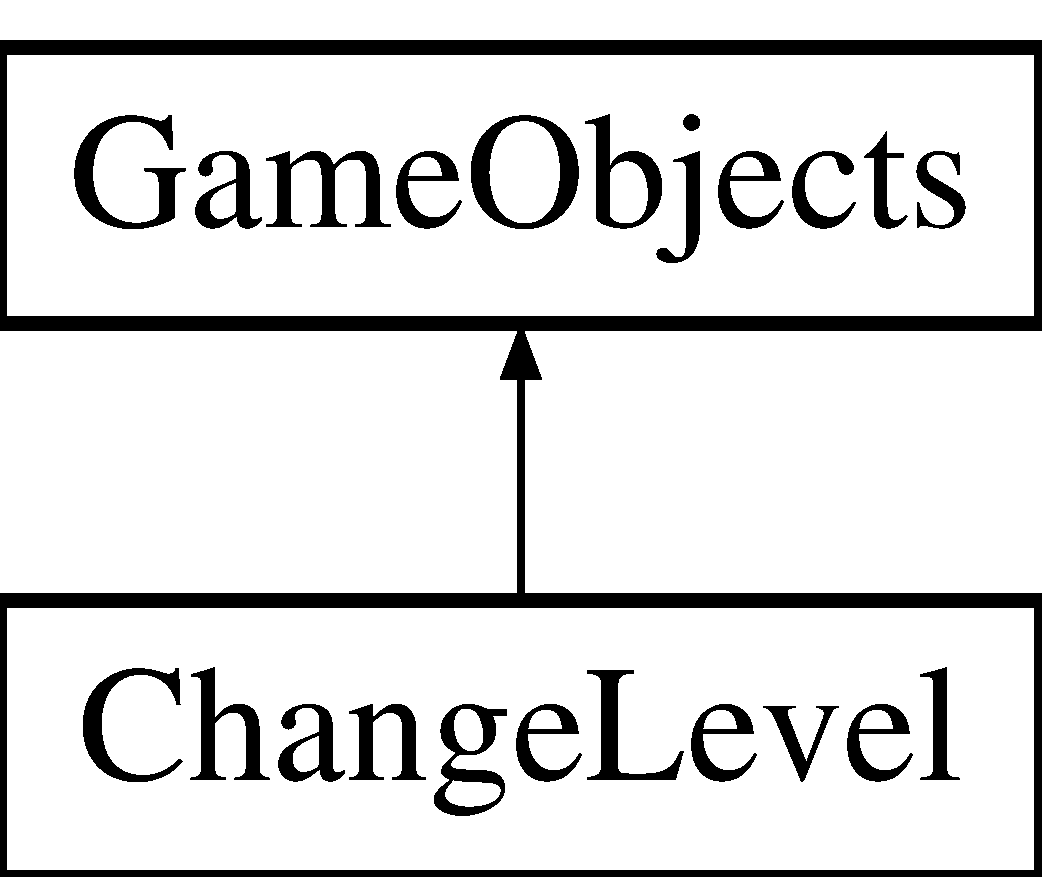
\includegraphics[height=2.000000cm]{classChangeLevel}
\end{center}
\end{figure}
\subsection*{Métodos públicos}
\begin{DoxyCompactItemize}
\item 
virtual \hyperlink{classEntity}{Entity} $\ast$ \hyperlink{classChangeLevel_aca170d1bbcbedf884246e48d9719fa89}{prepare\+Entity} (\hyperlink{classPropertyManager}{Property\+Manager} \&parameters)
\end{DoxyCompactItemize}


\subsection{Descripción detallada}
Constructor de una entidad concreta, un objeto del juego define una zona que provoca cambios de nivel 

\subsection{Documentación de las funciones miembro}
\hypertarget{classChangeLevel_aca170d1bbcbedf884246e48d9719fa89}{}\index{Change\+Level@{Change\+Level}!prepare\+Entity@{prepare\+Entity}}
\index{prepare\+Entity@{prepare\+Entity}!Change\+Level@{Change\+Level}}
\subsubsection[{prepare\+Entity}]{\setlength{\rightskip}{0pt plus 5cm}{\bf Entity} $\ast$ Change\+Level\+::prepare\+Entity (
\begin{DoxyParamCaption}
\item[{{\bf Property\+Manager} \&}]{parameters}
\end{DoxyParamCaption}
)\hspace{0.3cm}{\ttfamily [virtual]}}\label{classChangeLevel_aca170d1bbcbedf884246e48d9719fa89}
Devuelve una entidad que define una zona que provoca cambios de nivel dado unos parámetros 
\begin{DoxyParams}{Parámetros}
{\em parameters} & conjunto de parámetros \\
\hline
\end{DoxyParams}
\begin{DoxyReturn}{Devuelve}
entidad formada 
\end{DoxyReturn}


Implementa \hyperlink{classGameObjects_ad8d8177b229922b5a29e7355c8cf54ca}{Game\+Objects}.



La documentación para esta clase fue generada a partir de los siguientes ficheros\+:\begin{DoxyCompactItemize}
\item 
Change\+Level.\+h\item 
Change\+Level.\+cpp\end{DoxyCompactItemize}

\hypertarget{classCharacter}{}\section{Referencia de la Clase Character}
\label{classCharacter}\index{Character@{Character}}
Diagrama de herencias de Character\begin{figure}[H]
\begin{center}
\leavevmode
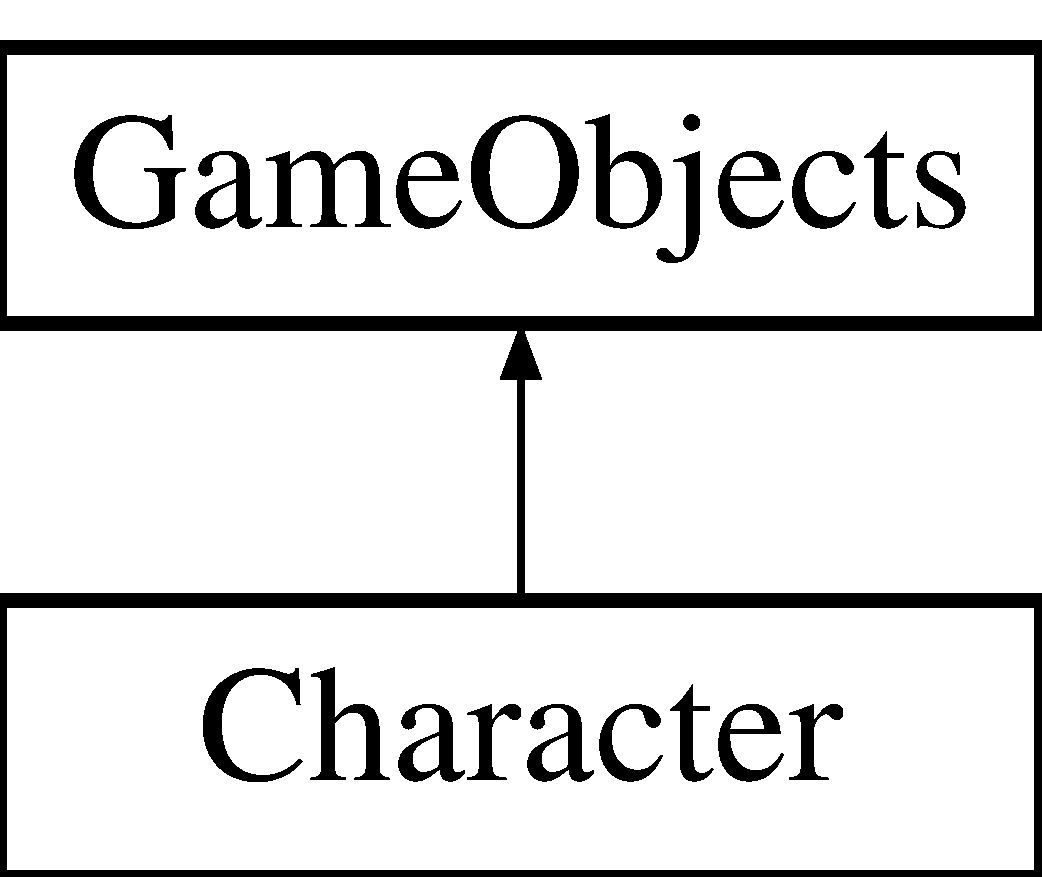
\includegraphics[height=2.000000cm]{classCharacter}
\end{center}
\end{figure}
\subsection*{Métodos públicos}
\begin{DoxyCompactItemize}
\item 
virtual \hyperlink{classEntity}{Entity} $\ast$ \hyperlink{classCharacter_adf409cd36c4f1cef03ded479451ebefe}{prepare\+Entity} (\hyperlink{classPropertyManager}{Property\+Manager} \&parameters)
\end{DoxyCompactItemize}


\subsection{Documentación de las funciones miembro}
\hypertarget{classCharacter_adf409cd36c4f1cef03ded479451ebefe}{}\index{Character@{Character}!prepare\+Entity@{prepare\+Entity}}
\index{prepare\+Entity@{prepare\+Entity}!Character@{Character}}
\subsubsection[{prepare\+Entity}]{\setlength{\rightskip}{0pt plus 5cm}{\bf Entity} $\ast$ Character\+::prepare\+Entity (
\begin{DoxyParamCaption}
\item[{{\bf Property\+Manager} \&}]{parameters}
\end{DoxyParamCaption}
)\hspace{0.3cm}{\ttfamily [virtual]}}\label{classCharacter_adf409cd36c4f1cef03ded479451ebefe}
Devuelve una entidad que define un protagonista dado unos parámetros 
\begin{DoxyParams}{Parámetros}
{\em parameters} & conjunto de parámetros \\
\hline
\end{DoxyParams}
\begin{DoxyReturn}{Devuelve}
entidad formada 
\end{DoxyReturn}


Implementa \hyperlink{classGameObjects_ad8d8177b229922b5a29e7355c8cf54ca}{Game\+Objects}.



La documentación para esta clase fue generada a partir de los siguientes ficheros\+:\begin{DoxyCompactItemize}
\item 
Character.\+h\item 
Character.\+cpp\end{DoxyCompactItemize}

\hypertarget{classClockHUD}{}\section{Referencia de la Clase Clock\+H\+U\+D}
\label{classClockHUD}\index{Clock\+H\+U\+D@{Clock\+H\+U\+D}}


{\ttfamily \#include $<$Clock\+H\+U\+D.\+h$>$}

Diagrama de herencias de Clock\+H\+U\+D\begin{figure}[H]
\begin{center}
\leavevmode
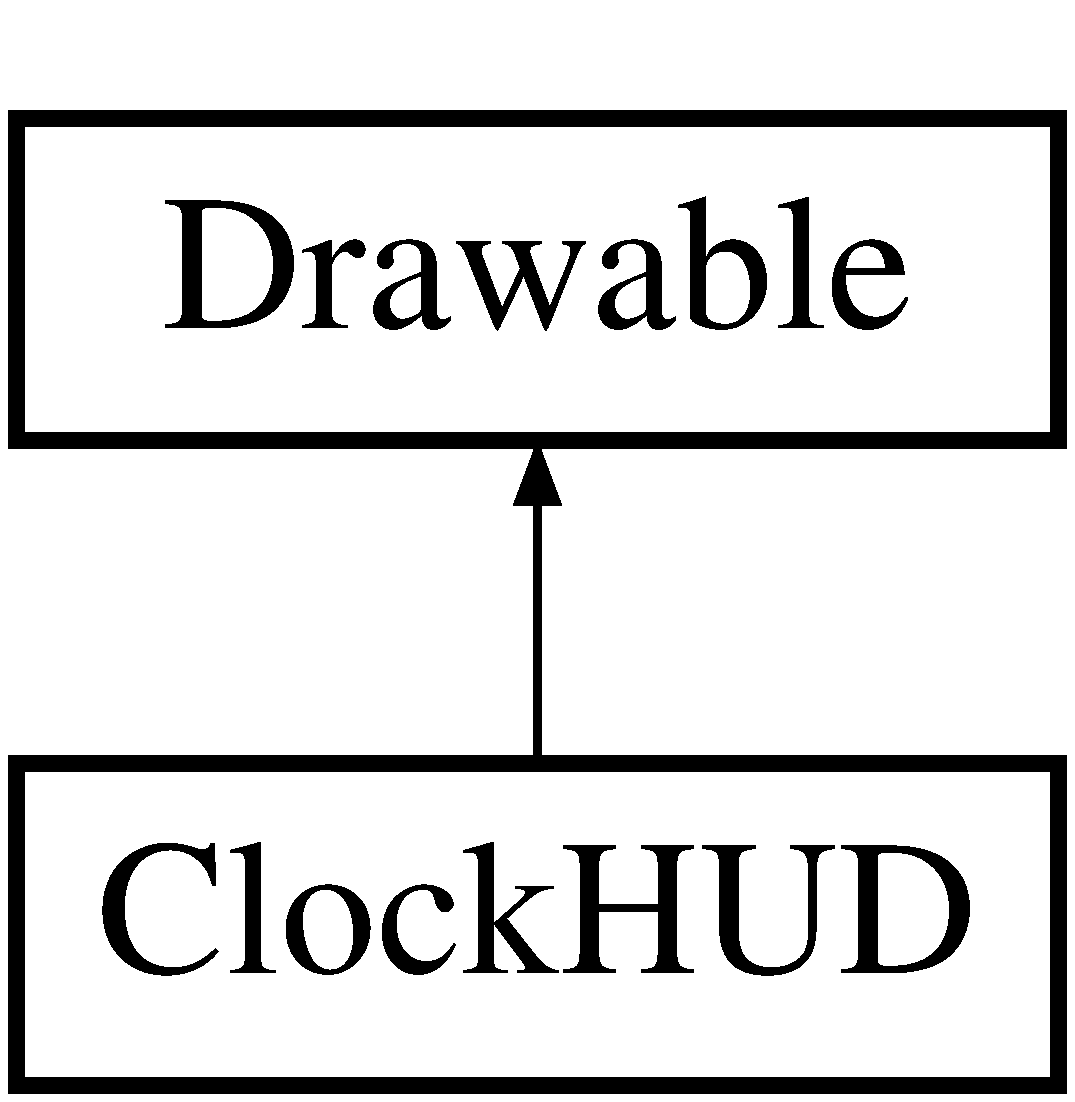
\includegraphics[height=2.000000cm]{classClockHUD}
\end{center}
\end{figure}
\subsection*{Métodos públicos}
\begin{DoxyCompactItemize}
\item 
\hyperlink{classClockHUD_a3f336b6ddd5619984bac27a18fb435b0}{Clock\+H\+U\+D} (const \hyperlink{classsfx_1_1FrameClock}{sfx\+::\+Frame\+Clock} \&clock, const sf\+::\+Font \&font)
\end{DoxyCompactItemize}


\subsection{Descripción detallada}
Interfaz a dibujar para mostrar estadísticas 

\subsection{Documentación del constructor y destructor}
\hypertarget{classClockHUD_a3f336b6ddd5619984bac27a18fb435b0}{}\index{Clock\+H\+U\+D@{Clock\+H\+U\+D}!Clock\+H\+U\+D@{Clock\+H\+U\+D}}
\index{Clock\+H\+U\+D@{Clock\+H\+U\+D}!Clock\+H\+U\+D@{Clock\+H\+U\+D}}
\subsubsection[{Clock\+H\+U\+D}]{\setlength{\rightskip}{0pt plus 5cm}Clock\+H\+U\+D\+::\+Clock\+H\+U\+D (
\begin{DoxyParamCaption}
\item[{const {\bf sfx\+::\+Frame\+Clock} \&}]{clock, }
\item[{const sf\+::\+Font \&}]{font}
\end{DoxyParamCaption}
)\hspace{0.3cm}{\ttfamily [inline]}}\label{classClockHUD_a3f336b6ddd5619984bac27a18fb435b0}
Constructor 
\begin{DoxyParams}{Parámetros}
{\em clock} & reloj de donde sacar los datos \\
\hline
{\em font} & fuente a usar para mostrar datos \\
\hline
\end{DoxyParams}


La documentación para esta clase fue generada a partir del siguiente fichero\+:\begin{DoxyCompactItemize}
\item 
Clock\+H\+U\+D.\+h\end{DoxyCompactItemize}

\hypertarget{classCollision}{}\section{Referencia de la Clase Collision}
\label{classCollision}\index{Collision@{Collision}}


{\ttfamily \#include $<$Collision.\+h$>$}

\subsection*{Métodos públicos}
\begin{DoxyCompactItemize}
\item 
\hyperlink{classCollision_aea8004fbf48b79b5db7b784688b23788}{Collision} ()
\item 
void \hyperlink{classCollision_aaf69e6b020eb9fd1cba8aec1d3bb859e}{add\+Vertice} (sf\+::\+Vertex \&vertex)
\item 
void \hyperlink{classCollision_a100a2d80f4163993669c06666255bc57}{add\+Array\+Vertex} (sf\+::\+Vertex\+Array \&array)
\item 
void \hyperlink{classCollision_a95e06a73baa76a87dc51ffca52fcc691}{set\+Array\+Vertex} (sf\+::\+Vertex\+Array $\ast$array)
\item 
void \hyperlink{classCollision_afb02271f321bcfa150098a19a07c8ee8}{update} (sf\+::\+Transformable \&transform)
\item 
void \hyperlink{classCollision_a72b8c24b2a8572c86620a75e048fd29b}{apply\+Ratio} (sf\+::\+Vector2f ratio)
\item 
sf\+::\+Transformable \hyperlink{classCollision_aecb16f7e4fd3e15a20679fedfbbde57d}{get\+Transform} ()
\item 
Type\+Collision \hyperlink{classCollision_a1f943423873c563bae17559933491afd}{get\+Type} () const 
\item 
void \hyperlink{classCollision_a16a681d155544e54068042cb2d97fbd4}{set\+Type} (Type\+Collision type)
\item 
sf\+::\+Float\+Rect \hyperlink{classCollision_af88eea50520b50648a3a6cc56ac81a67}{get\+A\+A\+B\+B} ()
\item 
sf\+::\+Float\+Rect \hyperlink{classCollision_aa0c3873dc05a248348fbe8bacf76213b}{get\+A\+A\+B\+B} (float time)
\item 
sf\+::\+Float\+Rect \hyperlink{classCollision_aa27c1d19aeb0b810be2e8016289d2d67}{get\+Previous\+A\+A\+B\+B} ()
\item 
sf\+::\+Float\+Rect \hyperlink{classCollision_ad650a86d63f7e85436f6df161b9c1857}{get\+A\+A\+B\+B\+Swept} ()
\end{DoxyCompactItemize}
\subsection*{Campos de datos}
\begin{DoxyCompactItemize}
\item 
sf\+::\+Vertex\+Array $\ast$ \hyperlink{classCollision_a6ba388302ae3971d876b0b06b00cab00}{vertices}
\end{DoxyCompactItemize}


\subsection{Descripción detallada}
Clase colisión, define una figura de colisión 

\subsection{Documentación del constructor y destructor}
\hypertarget{classCollision_aea8004fbf48b79b5db7b784688b23788}{}\index{Collision@{Collision}!Collision@{Collision}}
\index{Collision@{Collision}!Collision@{Collision}}
\subsubsection[{Collision}]{\setlength{\rightskip}{0pt plus 5cm}Collision\+::\+Collision (
\begin{DoxyParamCaption}
{}
\end{DoxyParamCaption}
)}\label{classCollision_aea8004fbf48b79b5db7b784688b23788}
Constructor por defecto 

\subsection{Documentación de las funciones miembro}
\hypertarget{classCollision_a100a2d80f4163993669c06666255bc57}{}\index{Collision@{Collision}!add\+Array\+Vertex@{add\+Array\+Vertex}}
\index{add\+Array\+Vertex@{add\+Array\+Vertex}!Collision@{Collision}}
\subsubsection[{add\+Array\+Vertex}]{\setlength{\rightskip}{0pt plus 5cm}void Collision\+::add\+Array\+Vertex (
\begin{DoxyParamCaption}
\item[{sf\+::\+Vertex\+Array \&}]{array}
\end{DoxyParamCaption}
)}\label{classCollision_a100a2d80f4163993669c06666255bc57}
Añade un array de vértices 
\begin{DoxyParams}{Parámetros}
{\em array} & de vértices \\
\hline
\end{DoxyParams}
\hypertarget{classCollision_aaf69e6b020eb9fd1cba8aec1d3bb859e}{}\index{Collision@{Collision}!add\+Vertice@{add\+Vertice}}
\index{add\+Vertice@{add\+Vertice}!Collision@{Collision}}
\subsubsection[{add\+Vertice}]{\setlength{\rightskip}{0pt plus 5cm}void Collision\+::add\+Vertice (
\begin{DoxyParamCaption}
\item[{sf\+::\+Vertex \&}]{vertex}
\end{DoxyParamCaption}
)}\label{classCollision_aaf69e6b020eb9fd1cba8aec1d3bb859e}
Añade vertice al colisionable 
\begin{DoxyParams}{Parámetros}
{\em vertex} & vértice \\
\hline
\end{DoxyParams}
\hypertarget{classCollision_a72b8c24b2a8572c86620a75e048fd29b}{}\index{Collision@{Collision}!apply\+Ratio@{apply\+Ratio}}
\index{apply\+Ratio@{apply\+Ratio}!Collision@{Collision}}
\subsubsection[{apply\+Ratio}]{\setlength{\rightskip}{0pt plus 5cm}void Collision\+::apply\+Ratio (
\begin{DoxyParamCaption}
\item[{sf\+::\+Vector2f}]{ratio}
\end{DoxyParamCaption}
)}\label{classCollision_a72b8c24b2a8572c86620a75e048fd29b}
Aplica un ratio de redimensionado a los vértices 
\begin{DoxyParams}{Parámetros}
{\em ratio} & \\
\hline
\end{DoxyParams}
\hypertarget{classCollision_af88eea50520b50648a3a6cc56ac81a67}{}\index{Collision@{Collision}!get\+A\+A\+B\+B@{get\+A\+A\+B\+B}}
\index{get\+A\+A\+B\+B@{get\+A\+A\+B\+B}!Collision@{Collision}}
\subsubsection[{get\+A\+A\+B\+B}]{\setlength{\rightskip}{0pt plus 5cm}sf\+::\+Float\+Rect Collision\+::get\+A\+A\+B\+B (
\begin{DoxyParamCaption}
{}
\end{DoxyParamCaption}
)}\label{classCollision_af88eea50520b50648a3a6cc56ac81a67}
Devuelve el rectángulo que contiene a los vértices \begin{DoxyReturn}{Devuelve}
rectángulo que contiene a los vértices 
\end{DoxyReturn}
\hypertarget{classCollision_aa0c3873dc05a248348fbe8bacf76213b}{}\index{Collision@{Collision}!get\+A\+A\+B\+B@{get\+A\+A\+B\+B}}
\index{get\+A\+A\+B\+B@{get\+A\+A\+B\+B}!Collision@{Collision}}
\subsubsection[{get\+A\+A\+B\+B}]{\setlength{\rightskip}{0pt plus 5cm}sf\+::\+Float\+Rect Collision\+::get\+A\+A\+B\+B (
\begin{DoxyParamCaption}
\item[{float}]{time}
\end{DoxyParamCaption}
)}\label{classCollision_aa0c3873dc05a248348fbe8bacf76213b}
Entre la posición anterior y la actual, devuelve el rectángulo que contiene a los vértices en el tiempo especificado 
\begin{DoxyParams}{Parámetros}
{\em time} & tiempo entre las posiciones \\
\hline
\end{DoxyParams}
\begin{DoxyReturn}{Devuelve}
rectángulo en el tiempo especificado 
\end{DoxyReturn}
\hypertarget{classCollision_ad650a86d63f7e85436f6df161b9c1857}{}\index{Collision@{Collision}!get\+A\+A\+B\+B\+Swept@{get\+A\+A\+B\+B\+Swept}}
\index{get\+A\+A\+B\+B\+Swept@{get\+A\+A\+B\+B\+Swept}!Collision@{Collision}}
\subsubsection[{get\+A\+A\+B\+B\+Swept}]{\setlength{\rightskip}{0pt plus 5cm}sf\+::\+Float\+Rect Collision\+::get\+A\+A\+B\+B\+Swept (
\begin{DoxyParamCaption}
{}
\end{DoxyParamCaption}
)}\label{classCollision_ad650a86d63f7e85436f6df161b9c1857}
Entre la posición anterior y la actual, devuelve el rectángulo formado entre los rectángulos de la posición anterior y la actual \begin{DoxyReturn}{Devuelve}
rectángulo entre ambas posiciones 
\end{DoxyReturn}
\hypertarget{classCollision_aa27c1d19aeb0b810be2e8016289d2d67}{}\index{Collision@{Collision}!get\+Previous\+A\+A\+B\+B@{get\+Previous\+A\+A\+B\+B}}
\index{get\+Previous\+A\+A\+B\+B@{get\+Previous\+A\+A\+B\+B}!Collision@{Collision}}
\subsubsection[{get\+Previous\+A\+A\+B\+B}]{\setlength{\rightskip}{0pt plus 5cm}sf\+::\+Float\+Rect Collision\+::get\+Previous\+A\+A\+B\+B (
\begin{DoxyParamCaption}
{}
\end{DoxyParamCaption}
)}\label{classCollision_aa27c1d19aeb0b810be2e8016289d2d67}
Devuelve el rectángulo que contiene a los vértices en la posición anterior \begin{DoxyReturn}{Devuelve}
rectángulo que contiene a los vértices en la posición anterior 
\end{DoxyReturn}
\hypertarget{classCollision_aecb16f7e4fd3e15a20679fedfbbde57d}{}\index{Collision@{Collision}!get\+Transform@{get\+Transform}}
\index{get\+Transform@{get\+Transform}!Collision@{Collision}}
\subsubsection[{get\+Transform}]{\setlength{\rightskip}{0pt plus 5cm}sf\+::\+Transformable Collision\+::get\+Transform (
\begin{DoxyParamCaption}
{}
\end{DoxyParamCaption}
)\hspace{0.3cm}{\ttfamily [inline]}}\label{classCollision_aecb16f7e4fd3e15a20679fedfbbde57d}
Devuelve las transformadas (posición, rotación y escalado) \begin{DoxyReturn}{Devuelve}
transformada 
\end{DoxyReturn}
\hypertarget{classCollision_a1f943423873c563bae17559933491afd}{}\index{Collision@{Collision}!get\+Type@{get\+Type}}
\index{get\+Type@{get\+Type}!Collision@{Collision}}
\subsubsection[{get\+Type}]{\setlength{\rightskip}{0pt plus 5cm}Type\+Collision Collision\+::get\+Type (
\begin{DoxyParamCaption}
{}
\end{DoxyParamCaption}
) const\hspace{0.3cm}{\ttfamily [inline]}}\label{classCollision_a1f943423873c563bae17559933491afd}
Devuelve el tipo de colisión \begin{DoxyReturn}{Devuelve}
tipo de colisión 
\end{DoxyReturn}
\hypertarget{classCollision_a95e06a73baa76a87dc51ffca52fcc691}{}\index{Collision@{Collision}!set\+Array\+Vertex@{set\+Array\+Vertex}}
\index{set\+Array\+Vertex@{set\+Array\+Vertex}!Collision@{Collision}}
\subsubsection[{set\+Array\+Vertex}]{\setlength{\rightskip}{0pt plus 5cm}void Collision\+::set\+Array\+Vertex (
\begin{DoxyParamCaption}
\item[{sf\+::\+Vertex\+Array $\ast$}]{array}
\end{DoxyParamCaption}
)}\label{classCollision_a95e06a73baa76a87dc51ffca52fcc691}
Setea el array de vértices 
\begin{DoxyParams}{Parámetros}
{\em array} & \\
\hline
\end{DoxyParams}
\hypertarget{classCollision_a16a681d155544e54068042cb2d97fbd4}{}\index{Collision@{Collision}!set\+Type@{set\+Type}}
\index{set\+Type@{set\+Type}!Collision@{Collision}}
\subsubsection[{set\+Type}]{\setlength{\rightskip}{0pt plus 5cm}void Collision\+::set\+Type (
\begin{DoxyParamCaption}
\item[{Type\+Collision}]{type}
\end{DoxyParamCaption}
)\hspace{0.3cm}{\ttfamily [inline]}}\label{classCollision_a16a681d155544e54068042cb2d97fbd4}
Setea el tipo de colisión 
\begin{DoxyParams}{Parámetros}
{\em type} & tipo de colisión \\
\hline
\end{DoxyParams}
\hypertarget{classCollision_afb02271f321bcfa150098a19a07c8ee8}{}\index{Collision@{Collision}!update@{update}}
\index{update@{update}!Collision@{Collision}}
\subsubsection[{update}]{\setlength{\rightskip}{0pt plus 5cm}void Collision\+::update (
\begin{DoxyParamCaption}
\item[{sf\+::\+Transformable \&}]{transform}
\end{DoxyParamCaption}
)}\label{classCollision_afb02271f321bcfa150098a19a07c8ee8}
Actualiza los vértices con la posición, rotación y escalado especificados 
\begin{DoxyParams}{Parámetros}
{\em transform} & posición, rotación y escalado \\
\hline
\end{DoxyParams}


\subsection{Documentación de los campos}
\hypertarget{classCollision_a6ba388302ae3971d876b0b06b00cab00}{}\index{Collision@{Collision}!vertices@{vertices}}
\index{vertices@{vertices}!Collision@{Collision}}
\subsubsection[{vertices}]{\setlength{\rightskip}{0pt plus 5cm}sf\+::\+Vertex\+Array$\ast$ Collision\+::vertices}\label{classCollision_a6ba388302ae3971d876b0b06b00cab00}
Vértices de la figura colisionable 

La documentación para esta clase fue generada a partir de los siguientes ficheros\+:\begin{DoxyCompactItemize}
\item 
Collision.\+h\item 
Collision.\+cpp\end{DoxyCompactItemize}

\hypertarget{structCommand}{}\section{Referencia de la Estructura Command}
\label{structCommand}\index{Command@{Command}}
\subsection*{Métodos públicos}
\begin{DoxyCompactItemize}
\item 
\hyperlink{structCommand_a18df2d81039392daeb0b78c346a70537}{Command} ()
\end{DoxyCompactItemize}
\subsection*{Campos de datos}
\begin{DoxyCompactItemize}
\item 
std\+::function$<$ void(\hyperlink{classEntity}{Entity} \&, sf\+::\+Time) $>$ \hyperlink{structCommand_ab4442395578bbfed1f3cebcb0923bec4}{action}
\item 
\hypertarget{structCommand_a1529e898c9e6dd47b1826b5b1eac09fb}{}unsigned int {\bfseries category}\label{structCommand_a1529e898c9e6dd47b1826b5b1eac09fb}

\end{DoxyCompactItemize}


\subsection{Documentación del constructor y destructor}
\hypertarget{structCommand_a18df2d81039392daeb0b78c346a70537}{}\index{Command@{Command}!Command@{Command}}
\index{Command@{Command}!Command@{Command}}
\subsubsection[{Command}]{\setlength{\rightskip}{0pt plus 5cm}Command\+::\+Command (
\begin{DoxyParamCaption}
{}
\end{DoxyParamCaption}
)}\label{structCommand_a18df2d81039392daeb0b78c346a70537}
C\+Onstructor 

\subsection{Documentación de los campos}
\hypertarget{structCommand_ab4442395578bbfed1f3cebcb0923bec4}{}\index{Command@{Command}!action@{action}}
\index{action@{action}!Command@{Command}}
\subsubsection[{action}]{\setlength{\rightskip}{0pt plus 5cm}std\+::function$<$void({\bf Entity}\&, sf\+::\+Time) $>$ Command\+::action}\label{structCommand_ab4442395578bbfed1f3cebcb0923bec4}
variable donde guardar la función a ejecutar 

La documentación para esta estructura fue generada a partir de los siguientes ficheros\+:\begin{DoxyCompactItemize}
\item 
Command.\+h\item 
Command.\+cpp\end{DoxyCompactItemize}

\hypertarget{classCommandQueue}{}\section{Referencia de la Clase Command\+Queue}
\label{classCommandQueue}\index{Command\+Queue@{Command\+Queue}}


{\ttfamily \#include $<$Command\+Queue.\+h$>$}

\subsection*{Métodos públicos}
\begin{DoxyCompactItemize}
\item 
void \hyperlink{classCommandQueue_ad444e0d7af45d9e09b834f0cec1e1f43}{push} (const \hyperlink{structCommand}{Command} \&command)
\item 
\hyperlink{structCommand}{Command} \hyperlink{classCommandQueue_ac2dde510222b8df393b55978f4594194}{pop} ()
\item 
bool \hyperlink{classCommandQueue_ad4f4731c185a293724a59aba9a5903d6}{is\+Empty} () const 
\end{DoxyCompactItemize}


\subsection{Descripción detallada}
Pila para los comandos 

\subsection{Documentación de las funciones miembro}
\hypertarget{classCommandQueue_ad4f4731c185a293724a59aba9a5903d6}{}\index{Command\+Queue@{Command\+Queue}!is\+Empty@{is\+Empty}}
\index{is\+Empty@{is\+Empty}!Command\+Queue@{Command\+Queue}}
\subsubsection[{is\+Empty}]{\setlength{\rightskip}{0pt plus 5cm}bool Command\+Queue\+::is\+Empty (
\begin{DoxyParamCaption}
{}
\end{DoxyParamCaption}
) const\hspace{0.3cm}{\ttfamily [inline]}}\label{classCommandQueue_ad4f4731c185a293724a59aba9a5903d6}
is empty \begin{DoxyReturn}{Devuelve}

\end{DoxyReturn}
\hypertarget{classCommandQueue_ac2dde510222b8df393b55978f4594194}{}\index{Command\+Queue@{Command\+Queue}!pop@{pop}}
\index{pop@{pop}!Command\+Queue@{Command\+Queue}}
\subsubsection[{pop}]{\setlength{\rightskip}{0pt plus 5cm}{\bf Command} Command\+Queue\+::pop (
\begin{DoxyParamCaption}
{}
\end{DoxyParamCaption}
)}\label{classCommandQueue_ac2dde510222b8df393b55978f4594194}
Pop command \begin{DoxyReturn}{Devuelve}
the command 
\end{DoxyReturn}
\hypertarget{classCommandQueue_ad444e0d7af45d9e09b834f0cec1e1f43}{}\index{Command\+Queue@{Command\+Queue}!push@{push}}
\index{push@{push}!Command\+Queue@{Command\+Queue}}
\subsubsection[{push}]{\setlength{\rightskip}{0pt plus 5cm}void Command\+Queue\+::push (
\begin{DoxyParamCaption}
\item[{const {\bf Command} \&}]{command}
\end{DoxyParamCaption}
)}\label{classCommandQueue_ad444e0d7af45d9e09b834f0cec1e1f43}
Add command 
\begin{DoxyParams}{Parámetros}
{\em command} & \\
\hline
\end{DoxyParams}


La documentación para esta clase fue generada a partir de los siguientes ficheros\+:\begin{DoxyCompactItemize}
\item 
Command\+Queue.\+h\item 
Command\+Queue.\+cpp\end{DoxyCompactItemize}

\hypertarget{classGUI_1_1Component}{}\section{Referencia de la Clase G\+U\+I\+:\+:Component}
\label{classGUI_1_1Component}\index{G\+U\+I\+::\+Component@{G\+U\+I\+::\+Component}}


{\ttfamily \#include $<$Component.\+h$>$}

Diagrama de herencias de G\+U\+I\+:\+:Component\begin{figure}[H]
\begin{center}
\leavevmode
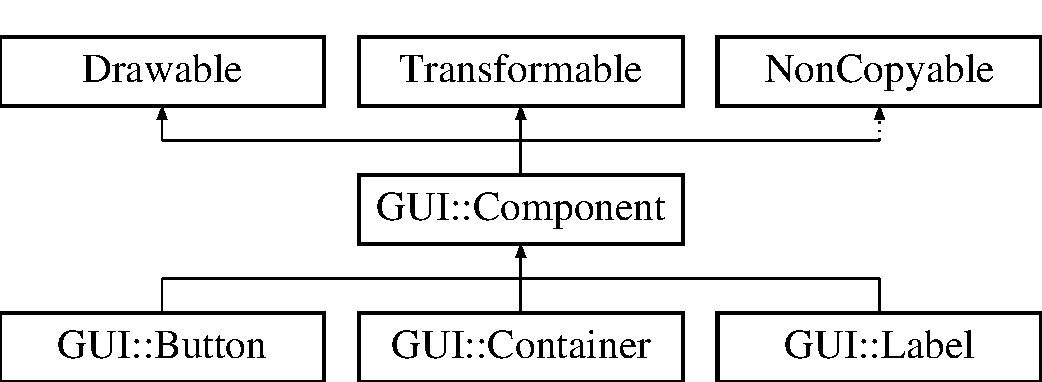
\includegraphics[height=3.000000cm]{classGUI_1_1Component}
\end{center}
\end{figure}
\subsection*{Métodos públicos}
\begin{DoxyCompactItemize}
\item 
\hyperlink{classGUI_1_1Component_a6a06664380a3d66ee8bcf3a41d760955}{Component} ()
\item 
virtual \hyperlink{classGUI_1_1Component_acb791835e060ed9743bc06bc6c7a7718}{$\sim$\+Component} ()
\item 
virtual bool \hyperlink{classGUI_1_1Component_a44d14506c9a1dbc839e05a6bf99c341b}{is\+Selectable} () const =0
\item 
bool \hyperlink{classGUI_1_1Component_affb93ae274f3dd3f44da70520d13b07d}{is\+Selected} () const 
\item 
virtual void \hyperlink{classGUI_1_1Component_ad0f7d6cc692edf2b0e426bfbd584be45}{select} ()
\item 
virtual void \hyperlink{classGUI_1_1Component_aa37424b238293bb308d357cf3b35c81f}{deselect} ()
\item 
virtual bool \hyperlink{classGUI_1_1Component_a74345f04fbeca17693f59d90bc0ae45b}{is\+Active} () const 
\item 
virtual void \hyperlink{classGUI_1_1Component_a965823e0e62612a7e532eb8c0b98861d}{activate} ()
\item 
virtual void \hyperlink{classGUI_1_1Component_a8964087afef859c015fb8188e619aa81}{deactivate} ()
\item 
virtual void \hyperlink{classGUI_1_1Component_aacf5e981e7b5726f5c7e9436455660ba}{handle\+Event} (const sf\+::\+Event \&event)=0
\end{DoxyCompactItemize}


\subsection{Descripción detallada}
Componente G\+U\+I, clase base 

\subsection{Documentación del constructor y destructor}
\hypertarget{classGUI_1_1Component_a6a06664380a3d66ee8bcf3a41d760955}{}\index{G\+U\+I\+::\+Component@{G\+U\+I\+::\+Component}!Component@{Component}}
\index{Component@{Component}!G\+U\+I\+::\+Component@{G\+U\+I\+::\+Component}}
\subsubsection[{Component}]{\setlength{\rightskip}{0pt plus 5cm}G\+U\+I\+::\+Component\+::\+Component (
\begin{DoxyParamCaption}
{}
\end{DoxyParamCaption}
)}\label{classGUI_1_1Component_a6a06664380a3d66ee8bcf3a41d760955}
Constructor \hypertarget{classGUI_1_1Component_acb791835e060ed9743bc06bc6c7a7718}{}\index{G\+U\+I\+::\+Component@{G\+U\+I\+::\+Component}!````~Component@{$\sim$\+Component}}
\index{````~Component@{$\sim$\+Component}!G\+U\+I\+::\+Component@{G\+U\+I\+::\+Component}}
\subsubsection[{$\sim$\+Component}]{\setlength{\rightskip}{0pt plus 5cm}G\+U\+I\+::\+Component\+::$\sim$\+Component (
\begin{DoxyParamCaption}
{}
\end{DoxyParamCaption}
)\hspace{0.3cm}{\ttfamily [virtual]}}\label{classGUI_1_1Component_acb791835e060ed9743bc06bc6c7a7718}
Destructor 

\subsection{Documentación de las funciones miembro}
\hypertarget{classGUI_1_1Component_a965823e0e62612a7e532eb8c0b98861d}{}\index{G\+U\+I\+::\+Component@{G\+U\+I\+::\+Component}!activate@{activate}}
\index{activate@{activate}!G\+U\+I\+::\+Component@{G\+U\+I\+::\+Component}}
\subsubsection[{activate}]{\setlength{\rightskip}{0pt plus 5cm}void G\+U\+I\+::\+Component\+::activate (
\begin{DoxyParamCaption}
{}
\end{DoxyParamCaption}
)\hspace{0.3cm}{\ttfamily [virtual]}}\label{classGUI_1_1Component_a965823e0e62612a7e532eb8c0b98861d}
Activa el componente 

Reimplementado en \hyperlink{classGUI_1_1Button_ad711a129863e0301c52b896911996123}{G\+U\+I\+::\+Button}.

\hypertarget{classGUI_1_1Component_a8964087afef859c015fb8188e619aa81}{}\index{G\+U\+I\+::\+Component@{G\+U\+I\+::\+Component}!deactivate@{deactivate}}
\index{deactivate@{deactivate}!G\+U\+I\+::\+Component@{G\+U\+I\+::\+Component}}
\subsubsection[{deactivate}]{\setlength{\rightskip}{0pt plus 5cm}void G\+U\+I\+::\+Component\+::deactivate (
\begin{DoxyParamCaption}
{}
\end{DoxyParamCaption}
)\hspace{0.3cm}{\ttfamily [virtual]}}\label{classGUI_1_1Component_a8964087afef859c015fb8188e619aa81}
Desactiva el componente 

Reimplementado en \hyperlink{classGUI_1_1Button_ab0a1773817447712b17ab1ad6da767da}{G\+U\+I\+::\+Button}.

\hypertarget{classGUI_1_1Component_aa37424b238293bb308d357cf3b35c81f}{}\index{G\+U\+I\+::\+Component@{G\+U\+I\+::\+Component}!deselect@{deselect}}
\index{deselect@{deselect}!G\+U\+I\+::\+Component@{G\+U\+I\+::\+Component}}
\subsubsection[{deselect}]{\setlength{\rightskip}{0pt plus 5cm}void G\+U\+I\+::\+Component\+::deselect (
\begin{DoxyParamCaption}
{}
\end{DoxyParamCaption}
)\hspace{0.3cm}{\ttfamily [virtual]}}\label{classGUI_1_1Component_aa37424b238293bb308d357cf3b35c81f}
Deselecciona el componente 

Reimplementado en \hyperlink{classGUI_1_1Button_a6fd040a471dc3ae48ad59cacd93c7292}{G\+U\+I\+::\+Button}.

\hypertarget{classGUI_1_1Component_aacf5e981e7b5726f5c7e9436455660ba}{}\index{G\+U\+I\+::\+Component@{G\+U\+I\+::\+Component}!handle\+Event@{handle\+Event}}
\index{handle\+Event@{handle\+Event}!G\+U\+I\+::\+Component@{G\+U\+I\+::\+Component}}
\subsubsection[{handle\+Event}]{\setlength{\rightskip}{0pt plus 5cm}virtual void G\+U\+I\+::\+Component\+::handle\+Event (
\begin{DoxyParamCaption}
\item[{const sf\+::\+Event \&}]{event}
\end{DoxyParamCaption}
)\hspace{0.3cm}{\ttfamily [pure virtual]}}\label{classGUI_1_1Component_aacf5e981e7b5726f5c7e9436455660ba}
Maneja los eventos capturados 
\begin{DoxyParams}{Parámetros}
{\em event} & evento capturado \\
\hline
\end{DoxyParams}


Implementado en \hyperlink{classGUI_1_1Button_a4d30e4caedd4c4373567ef452acd1fb1}{G\+U\+I\+::\+Button}, \hyperlink{classGUI_1_1Label_ade8d6fc5a2f56198764ee0ee0f216068}{G\+U\+I\+::\+Label} y \hyperlink{classGUI_1_1Container_af08db9d157a4e56f706493529901eb7f}{G\+U\+I\+::\+Container}.

\hypertarget{classGUI_1_1Component_a74345f04fbeca17693f59d90bc0ae45b}{}\index{G\+U\+I\+::\+Component@{G\+U\+I\+::\+Component}!is\+Active@{is\+Active}}
\index{is\+Active@{is\+Active}!G\+U\+I\+::\+Component@{G\+U\+I\+::\+Component}}
\subsubsection[{is\+Active}]{\setlength{\rightskip}{0pt plus 5cm}bool G\+U\+I\+::\+Component\+::is\+Active (
\begin{DoxyParamCaption}
{}
\end{DoxyParamCaption}
) const\hspace{0.3cm}{\ttfamily [virtual]}}\label{classGUI_1_1Component_a74345f04fbeca17693f59d90bc0ae45b}
Devuelve si el componente está activa \begin{DoxyReturn}{Devuelve}
true si está activo 
\end{DoxyReturn}
\hypertarget{classGUI_1_1Component_a44d14506c9a1dbc839e05a6bf99c341b}{}\index{G\+U\+I\+::\+Component@{G\+U\+I\+::\+Component}!is\+Selectable@{is\+Selectable}}
\index{is\+Selectable@{is\+Selectable}!G\+U\+I\+::\+Component@{G\+U\+I\+::\+Component}}
\subsubsection[{is\+Selectable}]{\setlength{\rightskip}{0pt plus 5cm}virtual bool G\+U\+I\+::\+Component\+::is\+Selectable (
\begin{DoxyParamCaption}
{}
\end{DoxyParamCaption}
) const\hspace{0.3cm}{\ttfamily [pure virtual]}}\label{classGUI_1_1Component_a44d14506c9a1dbc839e05a6bf99c341b}
Devuelve si el componente es seleccionable \begin{DoxyReturn}{Devuelve}
true si es seleccionable 
\end{DoxyReturn}


Implementado en \hyperlink{classGUI_1_1Button_a2fba8dea2886fd3bb33c7e250e695e8a}{G\+U\+I\+::\+Button}, \hyperlink{classGUI_1_1Container_a0780d6dc5502c171a8d35e97fa93122d}{G\+U\+I\+::\+Container} y \hyperlink{classGUI_1_1Label_a4bf3538b1d2ffa440c184ad59d9b9d76}{G\+U\+I\+::\+Label}.

\hypertarget{classGUI_1_1Component_affb93ae274f3dd3f44da70520d13b07d}{}\index{G\+U\+I\+::\+Component@{G\+U\+I\+::\+Component}!is\+Selected@{is\+Selected}}
\index{is\+Selected@{is\+Selected}!G\+U\+I\+::\+Component@{G\+U\+I\+::\+Component}}
\subsubsection[{is\+Selected}]{\setlength{\rightskip}{0pt plus 5cm}bool G\+U\+I\+::\+Component\+::is\+Selected (
\begin{DoxyParamCaption}
{}
\end{DoxyParamCaption}
) const}\label{classGUI_1_1Component_affb93ae274f3dd3f44da70520d13b07d}
Devuelve si el componente está seleccionado \begin{DoxyReturn}{Devuelve}
true si está seleccionado 
\end{DoxyReturn}
\hypertarget{classGUI_1_1Component_ad0f7d6cc692edf2b0e426bfbd584be45}{}\index{G\+U\+I\+::\+Component@{G\+U\+I\+::\+Component}!select@{select}}
\index{select@{select}!G\+U\+I\+::\+Component@{G\+U\+I\+::\+Component}}
\subsubsection[{select}]{\setlength{\rightskip}{0pt plus 5cm}void G\+U\+I\+::\+Component\+::select (
\begin{DoxyParamCaption}
{}
\end{DoxyParamCaption}
)\hspace{0.3cm}{\ttfamily [virtual]}}\label{classGUI_1_1Component_ad0f7d6cc692edf2b0e426bfbd584be45}
Selecciona el componente 

Reimplementado en \hyperlink{classGUI_1_1Button_a8f141129acb9c068ba6b8d19974d8291}{G\+U\+I\+::\+Button}.



La documentación para esta clase fue generada a partir de los siguientes ficheros\+:\begin{DoxyCompactItemize}
\item 
Component.\+h\item 
Component.\+cpp\end{DoxyCompactItemize}

\hypertarget{classGUI_1_1Container}{}\section{Referencia de la Clase G\+U\+I\+:\+:Container}
\label{classGUI_1_1Container}\index{G\+U\+I\+::\+Container@{G\+U\+I\+::\+Container}}


{\ttfamily \#include $<$Container.\+h$>$}

Diagrama de herencias de G\+U\+I\+:\+:Container\begin{figure}[H]
\begin{center}
\leavevmode
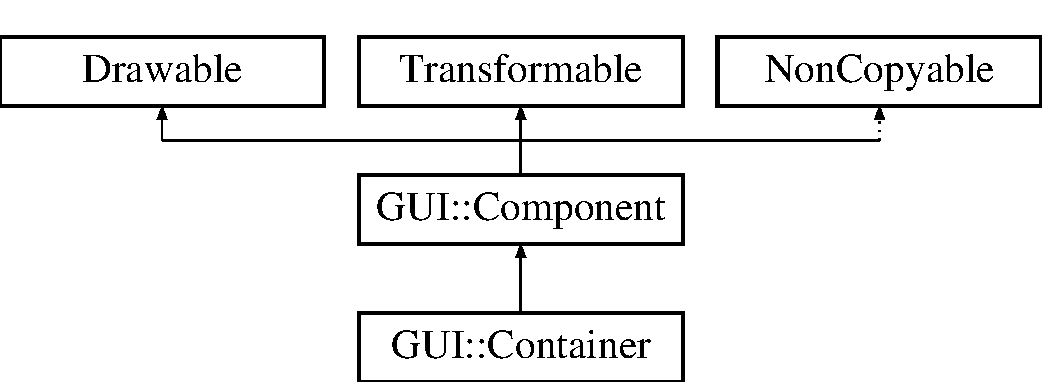
\includegraphics[height=3.000000cm]{classGUI_1_1Container}
\end{center}
\end{figure}
\subsection*{Métodos públicos}
\begin{DoxyCompactItemize}
\item 
\hyperlink{classGUI_1_1Container_a29ad430d6a9f0bebfea8567c91de1095}{Container} ()
\item 
virtual \hyperlink{classGUI_1_1Container_a6f08a80f950b90f542a2b29e980e7e79}{$\sim$\+Container} ()
\item 
void \hyperlink{classGUI_1_1Container_a9ed6e67b7c809fac99e30594d34a71c2}{pack} (\hyperlink{classGUI_1_1Component}{Component} $\ast$component)
\item 
virtual bool \hyperlink{classGUI_1_1Container_a0780d6dc5502c171a8d35e97fa93122d}{is\+Selectable} () const 
\item 
virtual void \hyperlink{classGUI_1_1Container_af08db9d157a4e56f706493529901eb7f}{handle\+Event} (const sf\+::\+Event \&event)
\item 
void \hyperlink{classGUI_1_1Container_a74aa11be28be40edc394fc585c335e74}{clear\+Selection} ()
\end{DoxyCompactItemize}


\subsection{Descripción detallada}
Contenedor G\+U\+I 

\subsection{Documentación del constructor y destructor}
\hypertarget{classGUI_1_1Container_a29ad430d6a9f0bebfea8567c91de1095}{}\index{G\+U\+I\+::\+Container@{G\+U\+I\+::\+Container}!Container@{Container}}
\index{Container@{Container}!G\+U\+I\+::\+Container@{G\+U\+I\+::\+Container}}
\subsubsection[{Container}]{\setlength{\rightskip}{0pt plus 5cm}G\+U\+I\+::\+Container\+::\+Container (
\begin{DoxyParamCaption}
{}
\end{DoxyParamCaption}
)}\label{classGUI_1_1Container_a29ad430d6a9f0bebfea8567c91de1095}
Constructor \hypertarget{classGUI_1_1Container_a6f08a80f950b90f542a2b29e980e7e79}{}\index{G\+U\+I\+::\+Container@{G\+U\+I\+::\+Container}!````~Container@{$\sim$\+Container}}
\index{````~Container@{$\sim$\+Container}!G\+U\+I\+::\+Container@{G\+U\+I\+::\+Container}}
\subsubsection[{$\sim$\+Container}]{\setlength{\rightskip}{0pt plus 5cm}G\+U\+I\+::\+Container\+::$\sim$\+Container (
\begin{DoxyParamCaption}
{}
\end{DoxyParamCaption}
)\hspace{0.3cm}{\ttfamily [virtual]}}\label{classGUI_1_1Container_a6f08a80f950b90f542a2b29e980e7e79}
Destructor 

\subsection{Documentación de las funciones miembro}
\hypertarget{classGUI_1_1Container_a74aa11be28be40edc394fc585c335e74}{}\index{G\+U\+I\+::\+Container@{G\+U\+I\+::\+Container}!clear\+Selection@{clear\+Selection}}
\index{clear\+Selection@{clear\+Selection}!G\+U\+I\+::\+Container@{G\+U\+I\+::\+Container}}
\subsubsection[{clear\+Selection}]{\setlength{\rightskip}{0pt plus 5cm}void G\+U\+I\+::\+Container\+::clear\+Selection (
\begin{DoxyParamCaption}
{}
\end{DoxyParamCaption}
)}\label{classGUI_1_1Container_a74aa11be28be40edc394fc585c335e74}
Limpia la seleccion del contenedor \hypertarget{classGUI_1_1Container_af08db9d157a4e56f706493529901eb7f}{}\index{G\+U\+I\+::\+Container@{G\+U\+I\+::\+Container}!handle\+Event@{handle\+Event}}
\index{handle\+Event@{handle\+Event}!G\+U\+I\+::\+Container@{G\+U\+I\+::\+Container}}
\subsubsection[{handle\+Event}]{\setlength{\rightskip}{0pt plus 5cm}void G\+U\+I\+::\+Container\+::handle\+Event (
\begin{DoxyParamCaption}
\item[{const sf\+::\+Event \&}]{event}
\end{DoxyParamCaption}
)\hspace{0.3cm}{\ttfamily [virtual]}}\label{classGUI_1_1Container_af08db9d157a4e56f706493529901eb7f}
Procesa la entrada 
\begin{DoxyParams}{Parámetros}
{\em event} & evento a procesar \\
\hline
\end{DoxyParams}


Implementa \hyperlink{classGUI_1_1Component_aacf5e981e7b5726f5c7e9436455660ba}{G\+U\+I\+::\+Component}.

\hypertarget{classGUI_1_1Container_a0780d6dc5502c171a8d35e97fa93122d}{}\index{G\+U\+I\+::\+Container@{G\+U\+I\+::\+Container}!is\+Selectable@{is\+Selectable}}
\index{is\+Selectable@{is\+Selectable}!G\+U\+I\+::\+Container@{G\+U\+I\+::\+Container}}
\subsubsection[{is\+Selectable}]{\setlength{\rightskip}{0pt plus 5cm}bool G\+U\+I\+::\+Container\+::is\+Selectable (
\begin{DoxyParamCaption}
{}
\end{DoxyParamCaption}
) const\hspace{0.3cm}{\ttfamily [virtual]}}\label{classGUI_1_1Container_a0780d6dc5502c171a8d35e97fa93122d}
Indica si es seleccionable el contenedor \begin{DoxyReturn}{Devuelve}
true si es seleccionable 
\end{DoxyReturn}


Implementa \hyperlink{classGUI_1_1Component_a44d14506c9a1dbc839e05a6bf99c341b}{G\+U\+I\+::\+Component}.

\hypertarget{classGUI_1_1Container_a9ed6e67b7c809fac99e30594d34a71c2}{}\index{G\+U\+I\+::\+Container@{G\+U\+I\+::\+Container}!pack@{pack}}
\index{pack@{pack}!G\+U\+I\+::\+Container@{G\+U\+I\+::\+Container}}
\subsubsection[{pack}]{\setlength{\rightskip}{0pt plus 5cm}void G\+U\+I\+::\+Container\+::pack (
\begin{DoxyParamCaption}
\item[{{\bf Component} $\ast$}]{component}
\end{DoxyParamCaption}
)}\label{classGUI_1_1Container_a9ed6e67b7c809fac99e30594d34a71c2}
Añade un componente al contenedor 
\begin{DoxyParams}{Parámetros}
{\em component} & componente a añadir \\
\hline
\end{DoxyParams}


La documentación para esta clase fue generada a partir de los siguientes ficheros\+:\begin{DoxyCompactItemize}
\item 
Container.\+h\item 
Container.\+cpp\end{DoxyCompactItemize}

\hypertarget{classContext}{}\section{Referencia de la Clase Context}
\label{classContext}\index{Context@{Context}}


{\ttfamily \#include $<$Context.\+h$>$}

\subsection*{Métodos públicos}
\begin{DoxyCompactItemize}
\item 
virtual \hyperlink{classContext_a2d34e4556448e40693f61d15e091b604}{$\sim$\+Context} ()
\item 
\hyperlink{classContext_a6e0630a0d56d8407216decee4add6d3f}{Context} (sf\+::\+Render\+Window \&window, \hyperlink{classResourceHolder}{Resource\+Holder}$<$ std\+::string, sf\+::\+Texture $>$ \&\hyperlink{classContext_a59ac23d12151de1912ab7f6d76e182b8}{textures}, \hyperlink{classResourceHolder}{Resource\+Holder}$<$ I\+D\+Fonts, sf\+::\+Font $>$ \&\hyperlink{classContext_a6e5b6ab3c18fc7f42f205774a597cdc1}{fonts}, \hyperlink{classPlayer}{Player} \&\hyperlink{classContext_a56c6b66908f8cb170e85a5a0e8dc6081}{player}, \hyperlink{classSystemManager}{System\+Manager} \&manager, \hyperlink{classMusicPlayer}{Music\+Player} \&\hyperlink{classContext_aaec563a152c2a98312c9f72a1b0a342a}{music}, \hyperlink{classSoundPlayer}{Sound\+Player} \&\hyperlink{classContext_ad83991aa701d0e22274e61e8bedb186f}{sounds}, std\+::string \&name)
\end{DoxyCompactItemize}
\subsection*{Campos de datos}
\begin{DoxyCompactItemize}
\item 
\hypertarget{classContext_adfd0cc74ffbdf3f22ae41f4114afb296}{}sf\+::\+Render\+Window $\ast$ {\bfseries window}\label{classContext_adfd0cc74ffbdf3f22ae41f4114afb296}

\item 
\hyperlink{classResourceHolder}{Resource\+Holder}$<$ std\+::string, sf\+::\+Texture $>$ $\ast$ \hyperlink{classContext_a59ac23d12151de1912ab7f6d76e182b8}{textures}
\item 
\hyperlink{classResourceHolder}{Resource\+Holder}$<$ I\+D\+Fonts, sf\+::\+Font $>$ $\ast$ \hyperlink{classContext_a6e5b6ab3c18fc7f42f205774a597cdc1}{fonts}
\item 
\hyperlink{classLevel}{Level} $\ast$ \hyperlink{classContext_ac7837bc30a1a062d5caab054ffedd917}{actual\+Level}
\item 
\hyperlink{classPlayer}{Player} $\ast$ \hyperlink{classContext_a56c6b66908f8cb170e85a5a0e8dc6081}{player}
\item 
\hyperlink{classSystemManager}{System\+Manager} $\ast$ \hyperlink{classContext_a7df558279371bada0354b48cd88353dc}{system\+Manager}
\item 
\hyperlink{classMusicPlayer}{Music\+Player} $\ast$ \hyperlink{classContext_aaec563a152c2a98312c9f72a1b0a342a}{music}
\item 
\hyperlink{classSoundPlayer}{Sound\+Player} $\ast$ \hyperlink{classContext_ad83991aa701d0e22274e61e8bedb186f}{sounds}
\item 
std\+::string $\ast$ \hyperlink{classContext_af675004382eab82f05bd95b5d614e6cf}{name\+Level}
\end{DoxyCompactItemize}


\subsection{Descripción detallada}
Contexto de la aplicación 

\subsection{Documentación del constructor y destructor}
\hypertarget{classContext_a2d34e4556448e40693f61d15e091b604}{}\index{Context@{Context}!````~Context@{$\sim$\+Context}}
\index{````~Context@{$\sim$\+Context}!Context@{Context}}
\subsubsection[{$\sim$\+Context}]{\setlength{\rightskip}{0pt plus 5cm}Context\+::$\sim$\+Context (
\begin{DoxyParamCaption}
{}
\end{DoxyParamCaption}
)\hspace{0.3cm}{\ttfamily [virtual]}}\label{classContext_a2d34e4556448e40693f61d15e091b604}
Destructor \hypertarget{classContext_a6e0630a0d56d8407216decee4add6d3f}{}\index{Context@{Context}!Context@{Context}}
\index{Context@{Context}!Context@{Context}}
\subsubsection[{Context}]{\setlength{\rightskip}{0pt plus 5cm}Context\+::\+Context (
\begin{DoxyParamCaption}
\item[{sf\+::\+Render\+Window \&}]{window, }
\item[{{\bf Resource\+Holder}$<$ std\+::string, sf\+::\+Texture $>$ \&}]{textures, }
\item[{{\bf Resource\+Holder}$<$ I\+D\+Fonts, sf\+::\+Font $>$ \&}]{fonts, }
\item[{{\bf Player} \&}]{player, }
\item[{{\bf System\+Manager} \&}]{manager, }
\item[{{\bf Music\+Player} \&}]{music, }
\item[{{\bf Sound\+Player} \&}]{sounds, }
\item[{std\+::string \&}]{name}
\end{DoxyParamCaption}
)}\label{classContext_a6e0630a0d56d8407216decee4add6d3f}
Constructor. Todos los parámetros que se le pasan están creados previamente 
\begin{DoxyParams}{Parámetros}
{\em window} & ventana de la aplicación \\
\hline
{\em textures} & texturas \\
\hline
{\em fonts} & fuentes \\
\hline
{\em player} & jugador \\
\hline
{\em manager} & gestor de sistemas \\
\hline
{\em music} & reproductor de música \\
\hline
{\em sounds} & reproductor de sonidos \\
\hline
{\em name} & nombre del nivel \\
\hline
\end{DoxyParams}


\subsection{Documentación de los campos}
\hypertarget{classContext_ac7837bc30a1a062d5caab054ffedd917}{}\index{Context@{Context}!actual\+Level@{actual\+Level}}
\index{actual\+Level@{actual\+Level}!Context@{Context}}
\subsubsection[{actual\+Level}]{\setlength{\rightskip}{0pt plus 5cm}{\bf Level}$\ast$ Context\+::actual\+Level}\label{classContext_ac7837bc30a1a062d5caab054ffedd917}
Nivel actual del juego \hypertarget{classContext_a6e5b6ab3c18fc7f42f205774a597cdc1}{}\index{Context@{Context}!fonts@{fonts}}
\index{fonts@{fonts}!Context@{Context}}
\subsubsection[{fonts}]{\setlength{\rightskip}{0pt plus 5cm}{\bf Resource\+Holder}$<$I\+D\+Fonts, sf\+::\+Font$>$$\ast$ Context\+::fonts}\label{classContext_a6e5b6ab3c18fc7f42f205774a597cdc1}
Fuentes \hypertarget{classContext_aaec563a152c2a98312c9f72a1b0a342a}{}\index{Context@{Context}!music@{music}}
\index{music@{music}!Context@{Context}}
\subsubsection[{music}]{\setlength{\rightskip}{0pt plus 5cm}{\bf Music\+Player}$\ast$ Context\+::music}\label{classContext_aaec563a152c2a98312c9f72a1b0a342a}
Reproductor de música \hypertarget{classContext_af675004382eab82f05bd95b5d614e6cf}{}\index{Context@{Context}!name\+Level@{name\+Level}}
\index{name\+Level@{name\+Level}!Context@{Context}}
\subsubsection[{name\+Level}]{\setlength{\rightskip}{0pt plus 5cm}std\+::string$\ast$ Context\+::name\+Level}\label{classContext_af675004382eab82f05bd95b5d614e6cf}
Nombre del nivel actual \hypertarget{classContext_a56c6b66908f8cb170e85a5a0e8dc6081}{}\index{Context@{Context}!player@{player}}
\index{player@{player}!Context@{Context}}
\subsubsection[{player}]{\setlength{\rightskip}{0pt plus 5cm}{\bf Player}$\ast$ Context\+::player}\label{classContext_a56c6b66908f8cb170e85a5a0e8dc6081}
Jugador \hypertarget{classContext_ad83991aa701d0e22274e61e8bedb186f}{}\index{Context@{Context}!sounds@{sounds}}
\index{sounds@{sounds}!Context@{Context}}
\subsubsection[{sounds}]{\setlength{\rightskip}{0pt plus 5cm}{\bf Sound\+Player}$\ast$ Context\+::sounds}\label{classContext_ad83991aa701d0e22274e61e8bedb186f}
Reproductor de sonidos \hypertarget{classContext_a7df558279371bada0354b48cd88353dc}{}\index{Context@{Context}!system\+Manager@{system\+Manager}}
\index{system\+Manager@{system\+Manager}!Context@{Context}}
\subsubsection[{system\+Manager}]{\setlength{\rightskip}{0pt plus 5cm}{\bf System\+Manager}$\ast$ Context\+::system\+Manager}\label{classContext_a7df558279371bada0354b48cd88353dc}
Sistemas del motor \hypertarget{classContext_a59ac23d12151de1912ab7f6d76e182b8}{}\index{Context@{Context}!textures@{textures}}
\index{textures@{textures}!Context@{Context}}
\subsubsection[{textures}]{\setlength{\rightskip}{0pt plus 5cm}{\bf Resource\+Holder}$<$std\+::string, sf\+::\+Texture$>$$\ast$ Context\+::textures}\label{classContext_a59ac23d12151de1912ab7f6d76e182b8}
Texturas 

La documentación para esta clase fue generada a partir de los siguientes ficheros\+:\begin{DoxyCompactItemize}
\item 
Context.\+h\item 
Context.\+cpp\end{DoxyCompactItemize}

\hypertarget{classConversationState}{}\section{Referencia de la Clase Conversation\+State}
\label{classConversationState}\index{Conversation\+State@{Conversation\+State}}


{\ttfamily \#include $<$Conversation\+State.\+h$>$}

Diagrama de herencias de Conversation\+State\begin{figure}[H]
\begin{center}
\leavevmode
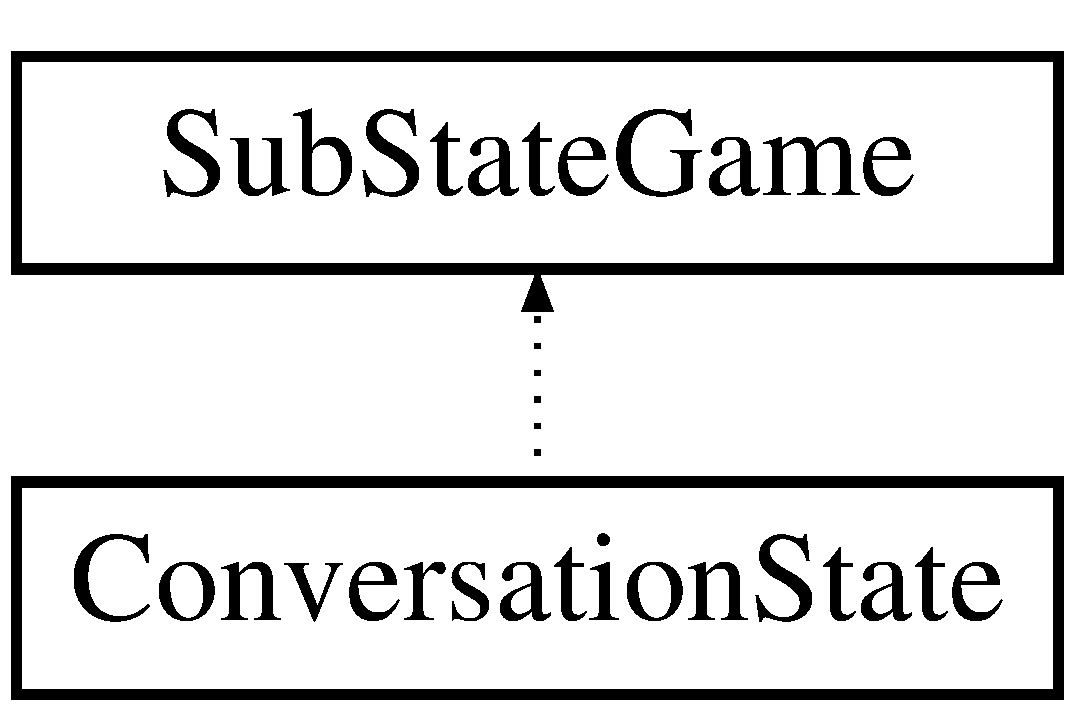
\includegraphics[height=2.000000cm]{classConversationState}
\end{center}
\end{figure}
\subsection*{Métodos públicos}
\begin{DoxyCompactItemize}
\item 
\hyperlink{classConversationState_a48512b6f1190aba61f243c4b1493778e}{Conversation\+State} (\hyperlink{classIdEntity}{Id\+Entity} id, \hyperlink{classSystemManager}{System\+Manager} $\ast$system)
\item 
\hypertarget{classConversationState_a0b2912e51f3be637027926e05c812820}{}virtual void {\bfseries draw} ()\label{classConversationState_a0b2912e51f3be637027926e05c812820}

\item 
\hypertarget{classConversationState_af509923e03dfe0abba9083e2b69d11af}{}virtual bool {\bfseries update} (sf\+::\+Time delta)\label{classConversationState_af509923e03dfe0abba9083e2b69d11af}

\item 
\hypertarget{classConversationState_a40e9dfb6b691cc962387b48c40feba16}{}virtual bool {\bfseries handle\+Event} (const sf\+::\+Event \&event)\label{classConversationState_a40e9dfb6b691cc962387b48c40feba16}

\end{DoxyCompactItemize}


\subsection{Descripción detallada}
Subestado para las conversaciones 

\subsection{Documentación del constructor y destructor}
\hypertarget{classConversationState_a48512b6f1190aba61f243c4b1493778e}{}\index{Conversation\+State@{Conversation\+State}!Conversation\+State@{Conversation\+State}}
\index{Conversation\+State@{Conversation\+State}!Conversation\+State@{Conversation\+State}}
\subsubsection[{Conversation\+State}]{\setlength{\rightskip}{0pt plus 5cm}Conversation\+State\+::\+Conversation\+State (
\begin{DoxyParamCaption}
\item[{{\bf Id\+Entity}}]{id, }
\item[{{\bf System\+Manager} $\ast$}]{system}
\end{DoxyParamCaption}
)}\label{classConversationState_a48512b6f1190aba61f243c4b1493778e}
Constructor 
\begin{DoxyParams}{Parámetros}
{\em id} & identificador de la entidad que habla \\
\hline
{\em system} & gestor de sistemas \\
\hline
\end{DoxyParams}


La documentación para esta clase fue generada a partir de los siguientes ficheros\+:\begin{DoxyCompactItemize}
\item 
Conversation\+State.\+h\item 
Conversation\+State.\+cpp\end{DoxyCompactItemize}

\hypertarget{unionDataUnion}{}\section{Referencia de la Unión Data\+Union}
\label{unionDataUnion}\index{Data\+Union@{Data\+Union}}


{\ttfamily \#include $<$Data\+Union.\+h$>$}

\subsection*{Campos de datos}
\begin{DoxyCompactItemize}
\item 
\hypertarget{unionDataUnion_a5705561f2e10c3bcc7596a451f67659b}{}\hyperlink{structStructPeople}{Struct\+People} $\ast$ {\bfseries people}\label{unionDataUnion_a5705561f2e10c3bcc7596a451f67659b}

\item 
\hypertarget{unionDataUnion_a1f06a482f7be35f5d6f7649649040e6c}{}\hyperlink{structStructMap}{Struct\+Map} $\ast$ {\bfseries map}\label{unionDataUnion_a1f06a482f7be35f5d6f7649649040e6c}

\item 
\hypertarget{unionDataUnion_a1a0bde2aa52acd09796f24853ae068a6}{}\hyperlink{classAnimation}{Animation} $\ast$ {\bfseries animation}\label{unionDataUnion_a1a0bde2aa52acd09796f24853ae068a6}

\item 
\hypertarget{unionDataUnion_a732b43c4b3d1915caf82680a51f5e7e5}{}\hyperlink{structStructAnimation}{Struct\+Animation} $\ast$ {\bfseries animations}\label{unionDataUnion_a732b43c4b3d1915caf82680a51f5e7e5}

\item 
\hypertarget{unionDataUnion_aeb971f7891fc8b2ecee5d745b0b89dc0}{}\hyperlink{classStateMachine}{State\+Machine} $\ast$ {\bfseries state\+Machine}\label{unionDataUnion_aeb971f7891fc8b2ecee5d745b0b89dc0}

\item 
\hypertarget{unionDataUnion_a50eaac3c29d6c6df2b81f5665a8a7afd}{}std\+::vector$<$ \hyperlink{structStructCollision}{Struct\+Collision} $\ast$ $>$ $\ast$ {\bfseries collisions}\label{unionDataUnion_a50eaac3c29d6c6df2b81f5665a8a7afd}

\item 
\hypertarget{unionDataUnion_a9ff0ceb279b1d158acc3f87c59f42f93}{}std\+::vector$<$ \hyperlink{classQuest}{Quest} $\ast$ $>$ $\ast$ {\bfseries quests}\label{unionDataUnion_a9ff0ceb279b1d158acc3f87c59f42f93}

\item 
\hypertarget{unionDataUnion_aa6918a8c6ec097e435dd7a415e392cdb}{}\hyperlink{classPropertyManager}{Property\+Manager} $\ast$ {\bfseries properties\+Entity}\label{unionDataUnion_aa6918a8c6ec097e435dd7a415e392cdb}

\end{DoxyCompactItemize}


\subsection{Descripción detallada}
Unión para guardar temporalmente los datos parseados de un xml 

La documentación para esta unión fue generada a partir del siguiente fichero\+:\begin{DoxyCompactItemize}
\item 
Data\+Union.\+h\end{DoxyCompactItemize}

\hypertarget{classDebug}{}\section{Referencia de la Clase Debug}
\label{classDebug}\index{Debug@{Debug}}


{\ttfamily \#include $<$Debug.\+h$>$}

Diagrama de herencias de Debug\begin{figure}[H]
\begin{center}
\leavevmode
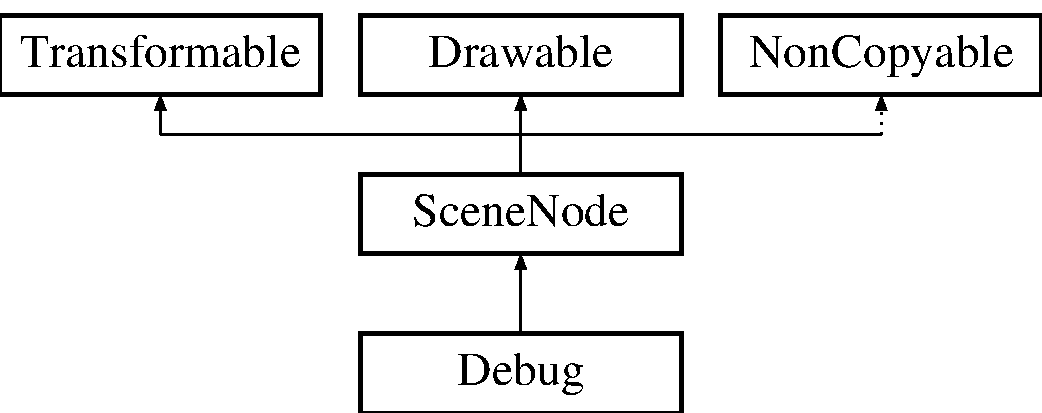
\includegraphics[height=3.000000cm]{classDebug}
\end{center}
\end{figure}
\subsection*{Métodos públicos}
\begin{DoxyCompactItemize}
\item 
\hyperlink{classDebug_afd64c07b6b7e27ee4997819a8207f40a}{Debug} (\hyperlink{classEntity}{Entity} $\ast$entity)
\item 
void \hyperlink{classDebug_ab858f1d67df563c9682a81152e1a61d2}{update\+Current} (sf\+::\+Time delta)
\item 
virtual void \hyperlink{classDebug_abbbe01dc7a7166ab745bac4760869acb}{draw\+Current} (sf\+::\+Render\+Target \&target, sf\+::\+Render\+States states) const 
\end{DoxyCompactItemize}
\subsection*{Otros miembros heredados}


\subsection{Descripción detallada}
Nodo utilizado para debug, en el se dibujan los puntos de colisión de la entidad 

\subsection{Documentación del constructor y destructor}
\hypertarget{classDebug_afd64c07b6b7e27ee4997819a8207f40a}{}\index{Debug@{Debug}!Debug@{Debug}}
\index{Debug@{Debug}!Debug@{Debug}}
\subsubsection[{Debug}]{\setlength{\rightskip}{0pt plus 5cm}Debug\+::\+Debug (
\begin{DoxyParamCaption}
\item[{{\bf Entity} $\ast$}]{entity}
\end{DoxyParamCaption}
)}\label{classDebug_afd64c07b6b7e27ee4997819a8207f40a}
Constructor 
\begin{DoxyParams}{Parámetros}
{\em entity} & entidad a comprobar su zona de colisión \\
\hline
\end{DoxyParams}


\subsection{Documentación de las funciones miembro}
\hypertarget{classDebug_abbbe01dc7a7166ab745bac4760869acb}{}\index{Debug@{Debug}!draw\+Current@{draw\+Current}}
\index{draw\+Current@{draw\+Current}!Debug@{Debug}}
\subsubsection[{draw\+Current}]{\setlength{\rightskip}{0pt plus 5cm}void Debug\+::draw\+Current (
\begin{DoxyParamCaption}
\item[{sf\+::\+Render\+Target \&}]{target, }
\item[{sf\+::\+Render\+States}]{states}
\end{DoxyParamCaption}
) const\hspace{0.3cm}{\ttfamily [virtual]}}\label{classDebug_abbbe01dc7a7166ab745bac4760869acb}
Draw the actual state of the node 
\begin{DoxyParams}{Parámetros}
{\em target} & \\
\hline
{\em states} & \\
\hline
\end{DoxyParams}


Reimplementado de \hyperlink{classSceneNode}{Scene\+Node}.

\hypertarget{classDebug_ab858f1d67df563c9682a81152e1a61d2}{}\index{Debug@{Debug}!update\+Current@{update\+Current}}
\index{update\+Current@{update\+Current}!Debug@{Debug}}
\subsubsection[{update\+Current}]{\setlength{\rightskip}{0pt plus 5cm}void Debug\+::update\+Current (
\begin{DoxyParamCaption}
\item[{sf\+::\+Time}]{delta}
\end{DoxyParamCaption}
)\hspace{0.3cm}{\ttfamily [virtual]}}\label{classDebug_ab858f1d67df563c9682a81152e1a61d2}
Actualiza la entidad/nodo 
\begin{DoxyParams}{Parámetros}
{\em delta} & tiempo entre frame y frame \\
\hline
\end{DoxyParams}


Reimplementado de \hyperlink{classSceneNode}{Scene\+Node}.



La documentación para esta clase fue generada a partir de los siguientes ficheros\+:\begin{DoxyCompactItemize}
\item 
Debug.\+h\item 
Debug.\+cpp\end{DoxyCompactItemize}

\hypertarget{classEntity}{}\section{Referencia de la Clase Entity}
\label{classEntity}\index{Entity@{Entity}}


{\ttfamily \#include $<$Entity.\+h$>$}

Diagrama de herencias de Entity\begin{figure}[H]
\begin{center}
\leavevmode
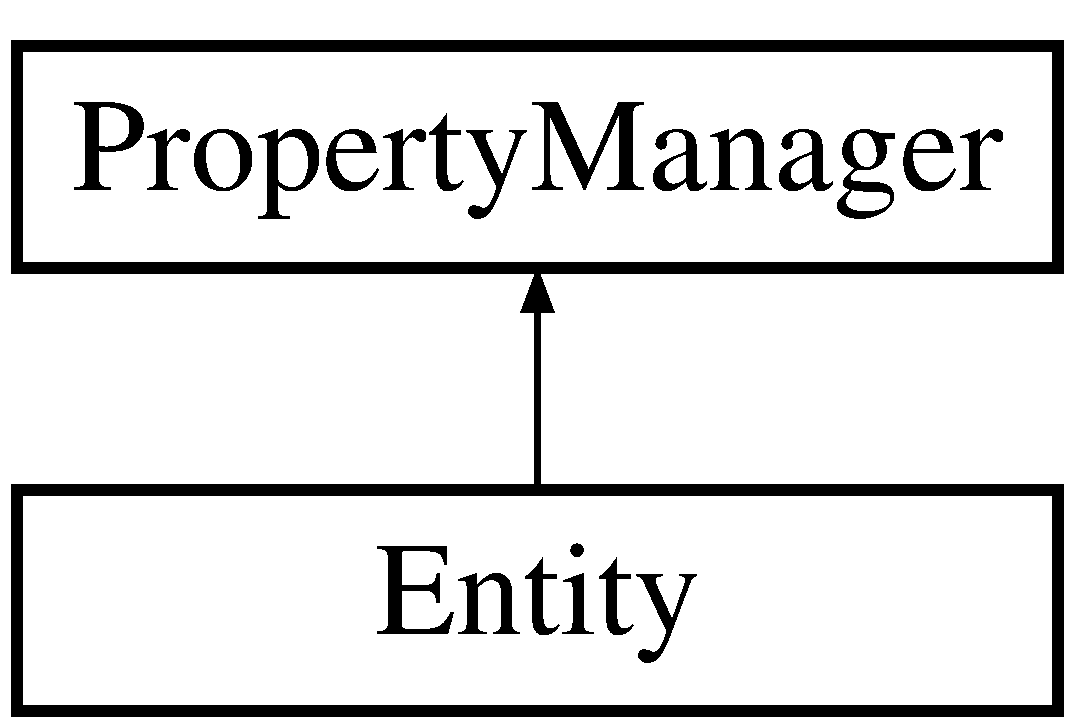
\includegraphics[height=2.000000cm]{classEntity}
\end{center}
\end{figure}
\subsection*{Métodos públicos}
\begin{DoxyCompactItemize}
\item 
\hyperlink{classEntity_a980f368aa07ce358583982821533a54a}{Entity} ()
\item 
\hyperlink{classEntity_ac015820cb62dac62532f4cff9e26374f}{Entity} (Category category)
\item 
virtual \hyperlink{classEntity_adf6d3f7cb1b2ba029b6b048a395cc8ae}{$\sim$\+Entity} ()
\item 
\hyperlink{classIdEntity}{Id\+Entity} \hyperlink{classEntity_afd7171167e43dab38b9b75f462fe234c}{get\+Id} () const 
\item 
void \hyperlink{classEntity_a8b7e893af5016e5ebff312abb6e7bbc0}{set\+Id} (\hyperlink{classIdEntity}{Id\+Entity} id)
\item 
bool \hyperlink{classEntity_a3c86039d4c16de3490b52a8595440f47}{is\+Destroyed} () const 
\item 
void \hyperlink{classEntity_a691dbe5f9ec930c27af2af0b97907a9e}{destroy} ()
\item 
Category \hyperlink{classEntity_a93708c98b4a7578b11b8c4f821484199}{get\+Category} () const 
\item 
\hyperlink{classIdEntity}{Id\+Entity} \hyperlink{classEntity_a9067f2ccad4931dc2a5b5dda1ce5180d}{get\+Id\+Xml} () const 
\item 
void \hyperlink{classEntity_abcc6d21fdca8f750c67a638cd1b32537}{set\+Id\+Xml} (\hyperlink{classIdEntity}{Id\+Entity} id)
\end{DoxyCompactItemize}


\subsection{Descripción detallada}
Entidad 

\subsection{Documentación del constructor y destructor}
\hypertarget{classEntity_a980f368aa07ce358583982821533a54a}{}\index{Entity@{Entity}!Entity@{Entity}}
\index{Entity@{Entity}!Entity@{Entity}}
\subsubsection[{Entity}]{\setlength{\rightskip}{0pt plus 5cm}Entity\+::\+Entity (
\begin{DoxyParamCaption}
{}
\end{DoxyParamCaption}
)}\label{classEntity_a980f368aa07ce358583982821533a54a}
Constructor \hypertarget{classEntity_ac015820cb62dac62532f4cff9e26374f}{}\index{Entity@{Entity}!Entity@{Entity}}
\index{Entity@{Entity}!Entity@{Entity}}
\subsubsection[{Entity}]{\setlength{\rightskip}{0pt plus 5cm}Entity\+::\+Entity (
\begin{DoxyParamCaption}
\item[{Category}]{category}
\end{DoxyParamCaption}
)}\label{classEntity_ac015820cb62dac62532f4cff9e26374f}
Constructor en el que se puede especificar la categoría a la que pertenece 
\begin{DoxyParams}{Parámetros}
{\em category} & categoria al que pertenece \\
\hline
\end{DoxyParams}
\hypertarget{classEntity_adf6d3f7cb1b2ba029b6b048a395cc8ae}{}\index{Entity@{Entity}!````~Entity@{$\sim$\+Entity}}
\index{````~Entity@{$\sim$\+Entity}!Entity@{Entity}}
\subsubsection[{$\sim$\+Entity}]{\setlength{\rightskip}{0pt plus 5cm}Entity\+::$\sim$\+Entity (
\begin{DoxyParamCaption}
{}
\end{DoxyParamCaption}
)\hspace{0.3cm}{\ttfamily [virtual]}}\label{classEntity_adf6d3f7cb1b2ba029b6b048a395cc8ae}
Destructor 

\subsection{Documentación de las funciones miembro}
\hypertarget{classEntity_a691dbe5f9ec930c27af2af0b97907a9e}{}\index{Entity@{Entity}!destroy@{destroy}}
\index{destroy@{destroy}!Entity@{Entity}}
\subsubsection[{destroy}]{\setlength{\rightskip}{0pt plus 5cm}void Entity\+::destroy (
\begin{DoxyParamCaption}
{}
\end{DoxyParamCaption}
)\hspace{0.3cm}{\ttfamily [inline]}}\label{classEntity_a691dbe5f9ec930c27af2af0b97907a9e}
Setea la entidad como destruida \hypertarget{classEntity_a93708c98b4a7578b11b8c4f821484199}{}\index{Entity@{Entity}!get\+Category@{get\+Category}}
\index{get\+Category@{get\+Category}!Entity@{Entity}}
\subsubsection[{get\+Category}]{\setlength{\rightskip}{0pt plus 5cm}Category Entity\+::get\+Category (
\begin{DoxyParamCaption}
{}
\end{DoxyParamCaption}
) const\hspace{0.3cm}{\ttfamily [inline]}}\label{classEntity_a93708c98b4a7578b11b8c4f821484199}
Devuelve la categoría de la entidad \begin{DoxyReturn}{Devuelve}
categoría de la entidad 
\end{DoxyReturn}
\hypertarget{classEntity_afd7171167e43dab38b9b75f462fe234c}{}\index{Entity@{Entity}!get\+Id@{get\+Id}}
\index{get\+Id@{get\+Id}!Entity@{Entity}}
\subsubsection[{get\+Id}]{\setlength{\rightskip}{0pt plus 5cm}{\bf Id\+Entity} Entity\+::get\+Id (
\begin{DoxyParamCaption}
{}
\end{DoxyParamCaption}
) const\hspace{0.3cm}{\ttfamily [inline]}}\label{classEntity_afd7171167e43dab38b9b75f462fe234c}
Devuelve el identificador de la entidad \begin{DoxyReturn}{Devuelve}
identificador de la entidad 
\end{DoxyReturn}
\hypertarget{classEntity_a9067f2ccad4931dc2a5b5dda1ce5180d}{}\index{Entity@{Entity}!get\+Id\+Xml@{get\+Id\+Xml}}
\index{get\+Id\+Xml@{get\+Id\+Xml}!Entity@{Entity}}
\subsubsection[{get\+Id\+Xml}]{\setlength{\rightskip}{0pt plus 5cm}{\bf Id\+Entity} Entity\+::get\+Id\+Xml (
\begin{DoxyParamCaption}
{}
\end{DoxyParamCaption}
) const\hspace{0.3cm}{\ttfamily [inline]}}\label{classEntity_a9067f2ccad4931dc2a5b5dda1ce5180d}
Devuelve el identificador de la entidad establecido en el xml de datos \begin{DoxyReturn}{Devuelve}
el identificador del xml de datos. Por defecto, es un id de -\/1 
\end{DoxyReturn}
\hypertarget{classEntity_a3c86039d4c16de3490b52a8595440f47}{}\index{Entity@{Entity}!is\+Destroyed@{is\+Destroyed}}
\index{is\+Destroyed@{is\+Destroyed}!Entity@{Entity}}
\subsubsection[{is\+Destroyed}]{\setlength{\rightskip}{0pt plus 5cm}bool Entity\+::is\+Destroyed (
\begin{DoxyParamCaption}
{}
\end{DoxyParamCaption}
) const\hspace{0.3cm}{\ttfamily [inline]}}\label{classEntity_a3c86039d4c16de3490b52a8595440f47}
Determina si la entidad está destruida \begin{DoxyReturn}{Devuelve}
true si la entidad está destruida 
\end{DoxyReturn}
\hypertarget{classEntity_a8b7e893af5016e5ebff312abb6e7bbc0}{}\index{Entity@{Entity}!set\+Id@{set\+Id}}
\index{set\+Id@{set\+Id}!Entity@{Entity}}
\subsubsection[{set\+Id}]{\setlength{\rightskip}{0pt plus 5cm}void Entity\+::set\+Id (
\begin{DoxyParamCaption}
\item[{{\bf Id\+Entity}}]{id}
\end{DoxyParamCaption}
)\hspace{0.3cm}{\ttfamily [inline]}}\label{classEntity_a8b7e893af5016e5ebff312abb6e7bbc0}
Setea el identificador de la entidad 
\begin{DoxyParams}{Parámetros}
{\em id} & nuevo identificador \\
\hline
\end{DoxyParams}
\hypertarget{classEntity_abcc6d21fdca8f750c67a638cd1b32537}{}\index{Entity@{Entity}!set\+Id\+Xml@{set\+Id\+Xml}}
\index{set\+Id\+Xml@{set\+Id\+Xml}!Entity@{Entity}}
\subsubsection[{set\+Id\+Xml}]{\setlength{\rightskip}{0pt plus 5cm}void Entity\+::set\+Id\+Xml (
\begin{DoxyParamCaption}
\item[{{\bf Id\+Entity}}]{id}
\end{DoxyParamCaption}
)\hspace{0.3cm}{\ttfamily [inline]}}\label{classEntity_abcc6d21fdca8f750c67a638cd1b32537}
Setea el identificador de la entidad establecido en el xml de datos 
\begin{DoxyParams}{Parámetros}
{\em id} & el identificador del xml de datos \\
\hline
\end{DoxyParams}


La documentación para esta clase fue generada a partir de los siguientes ficheros\+:\begin{DoxyCompactItemize}
\item 
Entity.\+h\item 
Entity.\+cpp\end{DoxyCompactItemize}

\hypertarget{classEntityNode}{}\section{Referencia de la Clase Entity\+Node}
\label{classEntityNode}\index{Entity\+Node@{Entity\+Node}}


{\ttfamily \#include $<$Entity\+Node.\+h$>$}

Diagrama de herencias de Entity\+Node\begin{figure}[H]
\begin{center}
\leavevmode
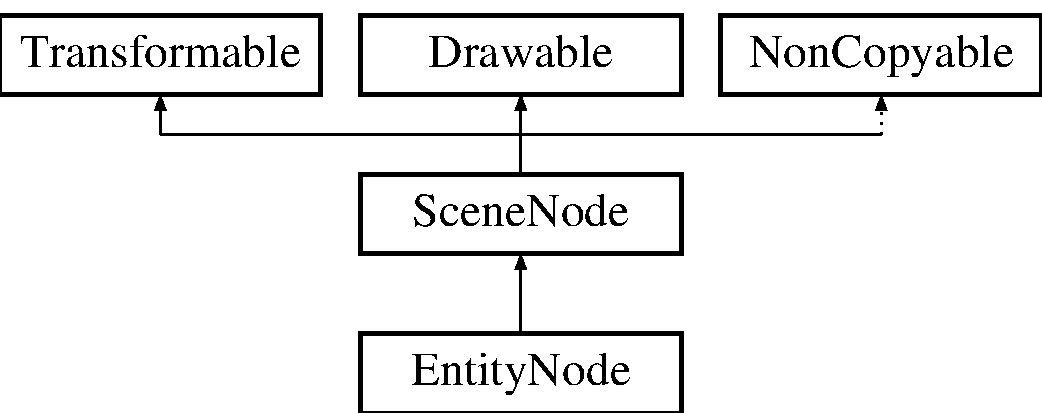
\includegraphics[height=3.000000cm]{classEntityNode}
\end{center}
\end{figure}
\subsection*{Métodos públicos}
\begin{DoxyCompactItemize}
\item 
\hyperlink{classEntityNode_adffc23015f30c960d0e02b9f51ff3742}{Entity\+Node} (\hyperlink{classEntity}{Entity} $\ast$entity)
\item 
\hyperlink{classEntity}{Entity} $\ast$ \hyperlink{classEntityNode_a5eb78668e4ff76d50aed68a9b6b028e2}{get\+Entity} () const 
\item 
virtual void \hyperlink{classEntityNode_afcda1234f815222781206bce3e41e67b}{draw\+Current} (sf\+::\+Render\+Target \&target, sf\+::\+Render\+States states) const 
\end{DoxyCompactItemize}
\subsection*{Métodos protegidos}
\begin{DoxyCompactItemize}
\item 
virtual void \hyperlink{classEntityNode_a1fdda1735246e22462e63b7872ddb972}{update\+Current} (sf\+::\+Time dt)
\item 
virtual void \hyperlink{classEntityNode_a90f8743448c763b4cd302dbbd2491bb0}{update\+Second\+Part} (sf\+::\+Time dt)
\end{DoxyCompactItemize}
\subsection*{Otros miembros heredados}


\subsection{Descripción detallada}
Nodo con una entidad 

\subsection{Documentación del constructor y destructor}
\hypertarget{classEntityNode_adffc23015f30c960d0e02b9f51ff3742}{}\index{Entity\+Node@{Entity\+Node}!Entity\+Node@{Entity\+Node}}
\index{Entity\+Node@{Entity\+Node}!Entity\+Node@{Entity\+Node}}
\subsubsection[{Entity\+Node}]{\setlength{\rightskip}{0pt plus 5cm}Entity\+Node\+::\+Entity\+Node (
\begin{DoxyParamCaption}
\item[{{\bf Entity} $\ast$}]{entity}
\end{DoxyParamCaption}
)}\label{classEntityNode_adffc23015f30c960d0e02b9f51ff3742}
Constructor 
\begin{DoxyParams}{Parámetros}
{\em entity} & entidad del nodo \\
\hline
\end{DoxyParams}


\subsection{Documentación de las funciones miembro}
\hypertarget{classEntityNode_afcda1234f815222781206bce3e41e67b}{}\index{Entity\+Node@{Entity\+Node}!draw\+Current@{draw\+Current}}
\index{draw\+Current@{draw\+Current}!Entity\+Node@{Entity\+Node}}
\subsubsection[{draw\+Current}]{\setlength{\rightskip}{0pt plus 5cm}void Entity\+Node\+::draw\+Current (
\begin{DoxyParamCaption}
\item[{sf\+::\+Render\+Target \&}]{target, }
\item[{sf\+::\+Render\+States}]{states}
\end{DoxyParamCaption}
) const\hspace{0.3cm}{\ttfamily [virtual]}}\label{classEntityNode_afcda1234f815222781206bce3e41e67b}
Inherit from \hyperlink{classSceneNode}{Scene\+Node}, draw the entity 
\begin{DoxyParams}{Parámetros}
{\em target} & \\
\hline
{\em states} & \\
\hline
\end{DoxyParams}


Reimplementado de \hyperlink{classSceneNode}{Scene\+Node}.

\hypertarget{classEntityNode_a5eb78668e4ff76d50aed68a9b6b028e2}{}\index{Entity\+Node@{Entity\+Node}!get\+Entity@{get\+Entity}}
\index{get\+Entity@{get\+Entity}!Entity\+Node@{Entity\+Node}}
\subsubsection[{get\+Entity}]{\setlength{\rightskip}{0pt plus 5cm}{\bf Entity}$\ast$ Entity\+Node\+::get\+Entity (
\begin{DoxyParamCaption}
{}
\end{DoxyParamCaption}
) const\hspace{0.3cm}{\ttfamily [inline]}}\label{classEntityNode_a5eb78668e4ff76d50aed68a9b6b028e2}
Devuelve la entidad del nodo \begin{DoxyReturn}{Devuelve}
entidad del nodo 
\end{DoxyReturn}
\hypertarget{classEntityNode_a1fdda1735246e22462e63b7872ddb972}{}\index{Entity\+Node@{Entity\+Node}!update\+Current@{update\+Current}}
\index{update\+Current@{update\+Current}!Entity\+Node@{Entity\+Node}}
\subsubsection[{update\+Current}]{\setlength{\rightskip}{0pt plus 5cm}void Entity\+Node\+::update\+Current (
\begin{DoxyParamCaption}
\item[{sf\+::\+Time}]{delta}
\end{DoxyParamCaption}
)\hspace{0.3cm}{\ttfamily [protected]}, {\ttfamily [virtual]}}\label{classEntityNode_a1fdda1735246e22462e63b7872ddb972}
Update the node with the time since last update 
\begin{DoxyParams}{Parámetros}
{\em delta} & \\
\hline
\end{DoxyParams}


Reimplementado de \hyperlink{classSceneNode}{Scene\+Node}.

\hypertarget{classEntityNode_a90f8743448c763b4cd302dbbd2491bb0}{}\index{Entity\+Node@{Entity\+Node}!update\+Second\+Part@{update\+Second\+Part}}
\index{update\+Second\+Part@{update\+Second\+Part}!Entity\+Node@{Entity\+Node}}
\subsubsection[{update\+Second\+Part}]{\setlength{\rightskip}{0pt plus 5cm}void Entity\+Node\+::update\+Second\+Part (
\begin{DoxyParamCaption}
\item[{sf\+::\+Time}]{dt}
\end{DoxyParamCaption}
)\hspace{0.3cm}{\ttfamily [protected]}, {\ttfamily [virtual]}}\label{classEntityNode_a90f8743448c763b4cd302dbbd2491bb0}
Actualiza la entidad/nodo en una segunda pasada 
\begin{DoxyParams}{Parámetros}
{\em dt} & tiempo entre frame y frame \\
\hline
\end{DoxyParams}


Reimplementado de \hyperlink{classSceneNode}{Scene\+Node}.



La documentación para esta clase fue generada a partir de los siguientes ficheros\+:\begin{DoxyCompactItemize}
\item 
Entity\+Node.\+h\item 
Entity\+Node.\+cpp\end{DoxyCompactItemize}

\hypertarget{classsfx_1_1FrameClock}{}\section{Referencia de la Clase sfx\+:\+:Frame\+Clock}
\label{classsfx_1_1FrameClock}\index{sfx\+::\+Frame\+Clock@{sfx\+::\+Frame\+Clock}}
\subsection*{Métodos públicos}
\begin{DoxyCompactItemize}
\item 
\hyperlink{classsfx_1_1FrameClock_a3a8d349a05fd1660e89aebdc10e9ce8e}{Frame\+Clock} (std\+::size\+\_\+t depth=100)
\item 
void \hyperlink{classsfx_1_1FrameClock_a5460df0fca7d2152c9495037ac3be951}{clear} ()
\item 
void \hyperlink{classsfx_1_1FrameClock_abbbf7925b85457baa38a5e58f4c59700}{begin\+Frame} ()
\item 
sf\+::\+Time \hyperlink{classsfx_1_1FrameClock_adc6c03afb4129e937135cc2c8c7efc85}{end\+Frame} ()
\item 
void \hyperlink{classsfx_1_1FrameClock_a2794e0ce9787e5ff728213990f25980b}{set\+Sample\+Depth} (std\+::size\+\_\+t depth)
\item 
std\+::size\+\_\+t \hyperlink{classsfx_1_1FrameClock_a4cbdd6b8e22258ef512484711cd815b6}{get\+Sample\+Depth} () const 
\item 
sf\+::\+Time \hyperlink{classsfx_1_1FrameClock_aae9f3f23f938cbb979f1b2192af12eae}{get\+Total\+Frame\+Time} () const 
\item 
sf\+::\+Uint64 \hyperlink{classsfx_1_1FrameClock_a27e3203a236bf84053702e878b62a3bd}{get\+Total\+Frame\+Count} () const 
\item 
sf\+::\+Time \hyperlink{classsfx_1_1FrameClock_a7ffe2e6262e3d47bcb80a9e56f57e6a7}{get\+Last\+Frame\+Time} () const 
\item 
sf\+::\+Time \hyperlink{classsfx_1_1FrameClock_ac34015580c6bbae9f4419027955a042a}{get\+Min\+Frame\+Time} () const 
\item 
sf\+::\+Time \hyperlink{classsfx_1_1FrameClock_a208707ee3920b0f0c8edd18edce7c663}{get\+Maxt\+Frame\+Time} () const 
\item 
sf\+::\+Time \hyperlink{classsfx_1_1FrameClock_aa7bac1e9ab95ea0409344f16d59daf07}{get\+Average\+Frame\+Time} () const 
\item 
float \hyperlink{classsfx_1_1FrameClock_a8b19e892d8ac098d7a7d3fdb1e4df4af}{get\+Frames\+Per\+Second} () const 
\item 
float \hyperlink{classsfx_1_1FrameClock_a09340f8787c0fdf244324ab14da893bd}{get\+Min\+Frames\+Per\+Second} () const 
\item 
float \hyperlink{classsfx_1_1FrameClock_a3aef85cda6ca3a238cdc886f379fcc3c}{get\+Max\+Frames\+Per\+Second} () const 
\item 
float \hyperlink{classsfx_1_1FrameClock_aec7b8a817abfeb934d5701776b50f9bc}{get\+Average\+Frames\+Per\+Second} () const 
\item 
void \hyperlink{classsfx_1_1FrameClock_add697719f9f2d5d01c67f52eabe2ef6e}{swap} (\hyperlink{classsfx_1_1FrameClock}{Frame\+Clock} \&other)
\end{DoxyCompactItemize}


\subsection{Documentación del constructor y destructor}
\hypertarget{classsfx_1_1FrameClock_a3a8d349a05fd1660e89aebdc10e9ce8e}{}\index{sfx\+::\+Frame\+Clock@{sfx\+::\+Frame\+Clock}!Frame\+Clock@{Frame\+Clock}}
\index{Frame\+Clock@{Frame\+Clock}!sfx\+::\+Frame\+Clock@{sfx\+::\+Frame\+Clock}}
\subsubsection[{Frame\+Clock}]{\setlength{\rightskip}{0pt plus 5cm}sfx\+::\+Frame\+Clock\+::\+Frame\+Clock (
\begin{DoxyParamCaption}
\item[{std\+::size\+\_\+t}]{depth = {\ttfamily 100}}
\end{DoxyParamCaption}
)\hspace{0.3cm}{\ttfamily [inline]}, {\ttfamily [explicit]}}\label{classsfx_1_1FrameClock_a3a8d349a05fd1660e89aebdc10e9ce8e}
Constructs a \hyperlink{classsfx_1_1FrameClock}{Frame\+Clock} object with sample depth \textquotesingle{}depth\textquotesingle{}. 
\begin{DoxyParams}{Parámetros}
{\em depth} & cantidad de frames como muestra \\
\hline
\end{DoxyParams}


\subsection{Documentación de las funciones miembro}
\hypertarget{classsfx_1_1FrameClock_abbbf7925b85457baa38a5e58f4c59700}{}\index{sfx\+::\+Frame\+Clock@{sfx\+::\+Frame\+Clock}!begin\+Frame@{begin\+Frame}}
\index{begin\+Frame@{begin\+Frame}!sfx\+::\+Frame\+Clock@{sfx\+::\+Frame\+Clock}}
\subsubsection[{begin\+Frame}]{\setlength{\rightskip}{0pt plus 5cm}void sfx\+::\+Frame\+Clock\+::begin\+Frame (
\begin{DoxyParamCaption}
{}
\end{DoxyParamCaption}
)\hspace{0.3cm}{\ttfamily [inline]}}\label{classsfx_1_1FrameClock_abbbf7925b85457baa38a5e58f4c59700}
Begin frame timing. Should be called once at the start of each new frame. \hypertarget{classsfx_1_1FrameClock_a5460df0fca7d2152c9495037ac3be951}{}\index{sfx\+::\+Frame\+Clock@{sfx\+::\+Frame\+Clock}!clear@{clear}}
\index{clear@{clear}!sfx\+::\+Frame\+Clock@{sfx\+::\+Frame\+Clock}}
\subsubsection[{clear}]{\setlength{\rightskip}{0pt plus 5cm}void sfx\+::\+Frame\+Clock\+::clear (
\begin{DoxyParamCaption}
{}
\end{DoxyParamCaption}
)\hspace{0.3cm}{\ttfamily [inline]}}\label{classsfx_1_1FrameClock_a5460df0fca7d2152c9495037ac3be951}
Resets all times to zero and discards accumulated samples. \hypertarget{classsfx_1_1FrameClock_adc6c03afb4129e937135cc2c8c7efc85}{}\index{sfx\+::\+Frame\+Clock@{sfx\+::\+Frame\+Clock}!end\+Frame@{end\+Frame}}
\index{end\+Frame@{end\+Frame}!sfx\+::\+Frame\+Clock@{sfx\+::\+Frame\+Clock}}
\subsubsection[{end\+Frame}]{\setlength{\rightskip}{0pt plus 5cm}sf\+::\+Time sfx\+::\+Frame\+Clock\+::end\+Frame (
\begin{DoxyParamCaption}
{}
\end{DoxyParamCaption}
)\hspace{0.3cm}{\ttfamily [inline]}}\label{classsfx_1_1FrameClock_adc6c03afb4129e937135cc2c8c7efc85}
End frame timing. Should be called once at the end of each frame.

\begin{DoxyReturn}{Devuelve}
Time elapsed since the matching \hyperlink{classsfx_1_1FrameClock_abbbf7925b85457baa38a5e58f4c59700}{Frame\+Clock\+::begin\+Frame}. 
\end{DoxyReturn}
\hypertarget{classsfx_1_1FrameClock_aec7b8a817abfeb934d5701776b50f9bc}{}\index{sfx\+::\+Frame\+Clock@{sfx\+::\+Frame\+Clock}!get\+Average\+Frames\+Per\+Second@{get\+Average\+Frames\+Per\+Second}}
\index{get\+Average\+Frames\+Per\+Second@{get\+Average\+Frames\+Per\+Second}!sfx\+::\+Frame\+Clock@{sfx\+::\+Frame\+Clock}}
\subsubsection[{get\+Average\+Frames\+Per\+Second}]{\setlength{\rightskip}{0pt plus 5cm}float sfx\+::\+Frame\+Clock\+::get\+Average\+Frames\+Per\+Second (
\begin{DoxyParamCaption}
{}
\end{DoxyParamCaption}
) const\hspace{0.3cm}{\ttfamily [inline]}}\label{classsfx_1_1FrameClock_aec7b8a817abfeb934d5701776b50f9bc}
\begin{DoxyReturn}{Devuelve}
Average frames per second over the last \hyperlink{classsfx_1_1FrameClock_a4cbdd6b8e22258ef512484711cd815b6}{get\+Sample\+Depth()} frames. 
\end{DoxyReturn}
\hypertarget{classsfx_1_1FrameClock_aa7bac1e9ab95ea0409344f16d59daf07}{}\index{sfx\+::\+Frame\+Clock@{sfx\+::\+Frame\+Clock}!get\+Average\+Frame\+Time@{get\+Average\+Frame\+Time}}
\index{get\+Average\+Frame\+Time@{get\+Average\+Frame\+Time}!sfx\+::\+Frame\+Clock@{sfx\+::\+Frame\+Clock}}
\subsubsection[{get\+Average\+Frame\+Time}]{\setlength{\rightskip}{0pt plus 5cm}sf\+::\+Time sfx\+::\+Frame\+Clock\+::get\+Average\+Frame\+Time (
\begin{DoxyParamCaption}
{}
\end{DoxyParamCaption}
) const\hspace{0.3cm}{\ttfamily [inline]}}\label{classsfx_1_1FrameClock_aa7bac1e9ab95ea0409344f16d59daf07}
\begin{DoxyReturn}{Devuelve}
Average frame time over the last \hyperlink{classsfx_1_1FrameClock_a4cbdd6b8e22258ef512484711cd815b6}{get\+Sample\+Depth()} frames. 
\end{DoxyReturn}
\hypertarget{classsfx_1_1FrameClock_a8b19e892d8ac098d7a7d3fdb1e4df4af}{}\index{sfx\+::\+Frame\+Clock@{sfx\+::\+Frame\+Clock}!get\+Frames\+Per\+Second@{get\+Frames\+Per\+Second}}
\index{get\+Frames\+Per\+Second@{get\+Frames\+Per\+Second}!sfx\+::\+Frame\+Clock@{sfx\+::\+Frame\+Clock}}
\subsubsection[{get\+Frames\+Per\+Second}]{\setlength{\rightskip}{0pt plus 5cm}float sfx\+::\+Frame\+Clock\+::get\+Frames\+Per\+Second (
\begin{DoxyParamCaption}
{}
\end{DoxyParamCaption}
) const\hspace{0.3cm}{\ttfamily [inline]}}\label{classsfx_1_1FrameClock_a8b19e892d8ac098d7a7d3fdb1e4df4af}
\begin{DoxyReturn}{Devuelve}
Frames per second, considering the pervious frame only. 
\end{DoxyReturn}
\hypertarget{classsfx_1_1FrameClock_a7ffe2e6262e3d47bcb80a9e56f57e6a7}{}\index{sfx\+::\+Frame\+Clock@{sfx\+::\+Frame\+Clock}!get\+Last\+Frame\+Time@{get\+Last\+Frame\+Time}}
\index{get\+Last\+Frame\+Time@{get\+Last\+Frame\+Time}!sfx\+::\+Frame\+Clock@{sfx\+::\+Frame\+Clock}}
\subsubsection[{get\+Last\+Frame\+Time}]{\setlength{\rightskip}{0pt plus 5cm}sf\+::\+Time sfx\+::\+Frame\+Clock\+::get\+Last\+Frame\+Time (
\begin{DoxyParamCaption}
{}
\end{DoxyParamCaption}
) const\hspace{0.3cm}{\ttfamily [inline]}}\label{classsfx_1_1FrameClock_a7ffe2e6262e3d47bcb80a9e56f57e6a7}
\begin{DoxyReturn}{Devuelve}
Time elapsed during the last \textquotesingle{}\hyperlink{classsfx_1_1FrameClock_abbbf7925b85457baa38a5e58f4c59700}{Frame\+Clock\+::begin\+Frame}/end\+Frame\textquotesingle{} pair. 
\end{DoxyReturn}
\hypertarget{classsfx_1_1FrameClock_a3aef85cda6ca3a238cdc886f379fcc3c}{}\index{sfx\+::\+Frame\+Clock@{sfx\+::\+Frame\+Clock}!get\+Max\+Frames\+Per\+Second@{get\+Max\+Frames\+Per\+Second}}
\index{get\+Max\+Frames\+Per\+Second@{get\+Max\+Frames\+Per\+Second}!sfx\+::\+Frame\+Clock@{sfx\+::\+Frame\+Clock}}
\subsubsection[{get\+Max\+Frames\+Per\+Second}]{\setlength{\rightskip}{0pt plus 5cm}float sfx\+::\+Frame\+Clock\+::get\+Max\+Frames\+Per\+Second (
\begin{DoxyParamCaption}
{}
\end{DoxyParamCaption}
) const\hspace{0.3cm}{\ttfamily [inline]}}\label{classsfx_1_1FrameClock_a3aef85cda6ca3a238cdc886f379fcc3c}
\begin{DoxyReturn}{Devuelve}
The highest measured frames per second. 
\end{DoxyReturn}
\hypertarget{classsfx_1_1FrameClock_a208707ee3920b0f0c8edd18edce7c663}{}\index{sfx\+::\+Frame\+Clock@{sfx\+::\+Frame\+Clock}!get\+Maxt\+Frame\+Time@{get\+Maxt\+Frame\+Time}}
\index{get\+Maxt\+Frame\+Time@{get\+Maxt\+Frame\+Time}!sfx\+::\+Frame\+Clock@{sfx\+::\+Frame\+Clock}}
\subsubsection[{get\+Maxt\+Frame\+Time}]{\setlength{\rightskip}{0pt plus 5cm}sf\+::\+Time sfx\+::\+Frame\+Clock\+::get\+Maxt\+Frame\+Time (
\begin{DoxyParamCaption}
{}
\end{DoxyParamCaption}
) const\hspace{0.3cm}{\ttfamily [inline]}}\label{classsfx_1_1FrameClock_a208707ee3920b0f0c8edd18edce7c663}
\begin{DoxyReturn}{Devuelve}
The longest measured frame time. 
\end{DoxyReturn}
\hypertarget{classsfx_1_1FrameClock_a09340f8787c0fdf244324ab14da893bd}{}\index{sfx\+::\+Frame\+Clock@{sfx\+::\+Frame\+Clock}!get\+Min\+Frames\+Per\+Second@{get\+Min\+Frames\+Per\+Second}}
\index{get\+Min\+Frames\+Per\+Second@{get\+Min\+Frames\+Per\+Second}!sfx\+::\+Frame\+Clock@{sfx\+::\+Frame\+Clock}}
\subsubsection[{get\+Min\+Frames\+Per\+Second}]{\setlength{\rightskip}{0pt plus 5cm}float sfx\+::\+Frame\+Clock\+::get\+Min\+Frames\+Per\+Second (
\begin{DoxyParamCaption}
{}
\end{DoxyParamCaption}
) const\hspace{0.3cm}{\ttfamily [inline]}}\label{classsfx_1_1FrameClock_a09340f8787c0fdf244324ab14da893bd}
\begin{DoxyReturn}{Devuelve}
The lowest measured frames per second. 
\end{DoxyReturn}
\hypertarget{classsfx_1_1FrameClock_ac34015580c6bbae9f4419027955a042a}{}\index{sfx\+::\+Frame\+Clock@{sfx\+::\+Frame\+Clock}!get\+Min\+Frame\+Time@{get\+Min\+Frame\+Time}}
\index{get\+Min\+Frame\+Time@{get\+Min\+Frame\+Time}!sfx\+::\+Frame\+Clock@{sfx\+::\+Frame\+Clock}}
\subsubsection[{get\+Min\+Frame\+Time}]{\setlength{\rightskip}{0pt plus 5cm}sf\+::\+Time sfx\+::\+Frame\+Clock\+::get\+Min\+Frame\+Time (
\begin{DoxyParamCaption}
{}
\end{DoxyParamCaption}
) const\hspace{0.3cm}{\ttfamily [inline]}}\label{classsfx_1_1FrameClock_ac34015580c6bbae9f4419027955a042a}
\begin{DoxyReturn}{Devuelve}
The shortest measured frame time. 
\end{DoxyReturn}
\hypertarget{classsfx_1_1FrameClock_a4cbdd6b8e22258ef512484711cd815b6}{}\index{sfx\+::\+Frame\+Clock@{sfx\+::\+Frame\+Clock}!get\+Sample\+Depth@{get\+Sample\+Depth}}
\index{get\+Sample\+Depth@{get\+Sample\+Depth}!sfx\+::\+Frame\+Clock@{sfx\+::\+Frame\+Clock}}
\subsubsection[{get\+Sample\+Depth}]{\setlength{\rightskip}{0pt plus 5cm}std\+::size\+\_\+t sfx\+::\+Frame\+Clock\+::get\+Sample\+Depth (
\begin{DoxyParamCaption}
{}
\end{DoxyParamCaption}
) const\hspace{0.3cm}{\ttfamily [inline]}}\label{classsfx_1_1FrameClock_a4cbdd6b8e22258ef512484711cd815b6}
\begin{DoxyReturn}{Devuelve}
The number of frames to be sampled for averaging. 
\end{DoxyReturn}
\hypertarget{classsfx_1_1FrameClock_a27e3203a236bf84053702e878b62a3bd}{}\index{sfx\+::\+Frame\+Clock@{sfx\+::\+Frame\+Clock}!get\+Total\+Frame\+Count@{get\+Total\+Frame\+Count}}
\index{get\+Total\+Frame\+Count@{get\+Total\+Frame\+Count}!sfx\+::\+Frame\+Clock@{sfx\+::\+Frame\+Clock}}
\subsubsection[{get\+Total\+Frame\+Count}]{\setlength{\rightskip}{0pt plus 5cm}sf\+::\+Uint64 sfx\+::\+Frame\+Clock\+::get\+Total\+Frame\+Count (
\begin{DoxyParamCaption}
{}
\end{DoxyParamCaption}
) const\hspace{0.3cm}{\ttfamily [inline]}}\label{classsfx_1_1FrameClock_a27e3203a236bf84053702e878b62a3bd}
\begin{DoxyReturn}{Devuelve}
The total accumulated number of frames. 
\end{DoxyReturn}
\hypertarget{classsfx_1_1FrameClock_aae9f3f23f938cbb979f1b2192af12eae}{}\index{sfx\+::\+Frame\+Clock@{sfx\+::\+Frame\+Clock}!get\+Total\+Frame\+Time@{get\+Total\+Frame\+Time}}
\index{get\+Total\+Frame\+Time@{get\+Total\+Frame\+Time}!sfx\+::\+Frame\+Clock@{sfx\+::\+Frame\+Clock}}
\subsubsection[{get\+Total\+Frame\+Time}]{\setlength{\rightskip}{0pt plus 5cm}sf\+::\+Time sfx\+::\+Frame\+Clock\+::get\+Total\+Frame\+Time (
\begin{DoxyParamCaption}
{}
\end{DoxyParamCaption}
) const\hspace{0.3cm}{\ttfamily [inline]}}\label{classsfx_1_1FrameClock_aae9f3f23f938cbb979f1b2192af12eae}
\begin{DoxyReturn}{Devuelve}
The total accumulated frame time. 
\end{DoxyReturn}
\hypertarget{classsfx_1_1FrameClock_a2794e0ce9787e5ff728213990f25980b}{}\index{sfx\+::\+Frame\+Clock@{sfx\+::\+Frame\+Clock}!set\+Sample\+Depth@{set\+Sample\+Depth}}
\index{set\+Sample\+Depth@{set\+Sample\+Depth}!sfx\+::\+Frame\+Clock@{sfx\+::\+Frame\+Clock}}
\subsubsection[{set\+Sample\+Depth}]{\setlength{\rightskip}{0pt plus 5cm}void sfx\+::\+Frame\+Clock\+::set\+Sample\+Depth (
\begin{DoxyParamCaption}
\item[{std\+::size\+\_\+t}]{depth}
\end{DoxyParamCaption}
)\hspace{0.3cm}{\ttfamily [inline]}}\label{classsfx_1_1FrameClock_a2794e0ce9787e5ff728213990f25980b}
Sets the number of frames to be sampled for averaging. \textquotesingle{}depth\textquotesingle{} must be greater than or equal to 1. 
\begin{DoxyParams}{Parámetros}
{\em depth} & \\
\hline
\end{DoxyParams}
\hypertarget{classsfx_1_1FrameClock_add697719f9f2d5d01c67f52eabe2ef6e}{}\index{sfx\+::\+Frame\+Clock@{sfx\+::\+Frame\+Clock}!swap@{swap}}
\index{swap@{swap}!sfx\+::\+Frame\+Clock@{sfx\+::\+Frame\+Clock}}
\subsubsection[{swap}]{\setlength{\rightskip}{0pt plus 5cm}void sfx\+::\+Frame\+Clock\+::swap (
\begin{DoxyParamCaption}
\item[{{\bf Frame\+Clock} \&}]{other}
\end{DoxyParamCaption}
)\hspace{0.3cm}{\ttfamily [inline]}}\label{classsfx_1_1FrameClock_add697719f9f2d5d01c67f52eabe2ef6e}
Swaps the value of this \hyperlink{classsfx_1_1FrameClock}{Frame\+Clock} instance with \textquotesingle{}other\textquotesingle{}. 
\begin{DoxyParams}{Parámetros}
{\em other} & other frameclock instance \\
\hline
\end{DoxyParams}


La documentación para esta clase fue generada a partir del siguiente fichero\+:\begin{DoxyCompactItemize}
\item 
Frame\+Clock.\+h\end{DoxyCompactItemize}

\hypertarget{classGameObjects}{}\section{Referencia de la Clase Game\+Objects}
\label{classGameObjects}\index{Game\+Objects@{Game\+Objects}}


{\ttfamily \#include $<$Game\+Objects.\+h$>$}

Diagrama de herencias de Game\+Objects\begin{figure}[H]
\begin{center}
\leavevmode
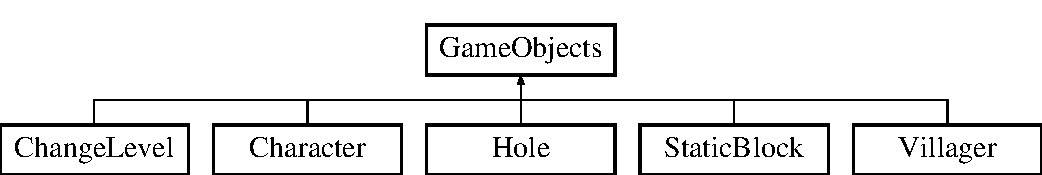
\includegraphics[height=2.000000cm]{classGameObjects}
\end{center}
\end{figure}
\subsection*{Métodos públicos}
\begin{DoxyCompactItemize}
\item 
virtual \hyperlink{classEntity}{Entity} $\ast$ \hyperlink{classGameObjects_ad8d8177b229922b5a29e7355c8cf54ca}{prepare\+Entity} (\hyperlink{classPropertyManager}{Property\+Manager} \&parameters)=0
\end{DoxyCompactItemize}


\subsection{Descripción detallada}
Clase base para todos los objetos del juego 

\subsection{Documentación de las funciones miembro}
\hypertarget{classGameObjects_ad8d8177b229922b5a29e7355c8cf54ca}{}\index{Game\+Objects@{Game\+Objects}!prepare\+Entity@{prepare\+Entity}}
\index{prepare\+Entity@{prepare\+Entity}!Game\+Objects@{Game\+Objects}}
\subsubsection[{prepare\+Entity}]{\setlength{\rightskip}{0pt plus 5cm}virtual {\bf Entity}$\ast$ Game\+Objects\+::prepare\+Entity (
\begin{DoxyParamCaption}
\item[{{\bf Property\+Manager} \&}]{parameters}
\end{DoxyParamCaption}
)\hspace{0.3cm}{\ttfamily [pure virtual]}}\label{classGameObjects_ad8d8177b229922b5a29e7355c8cf54ca}
Devuelve una entidad que define objeto del juego 
\begin{DoxyParams}{Parámetros}
{\em parameters} & conjunto de parámetros \\
\hline
\end{DoxyParams}
\begin{DoxyReturn}{Devuelve}
entidad formada 
\end{DoxyReturn}


Implementado en \hyperlink{classVillager_a8407dc0b40215058d81a3b83895529f9}{Villager}, \hyperlink{classChangeLevel_aca170d1bbcbedf884246e48d9719fa89}{Change\+Level}, \hyperlink{classHole_a972b6c3658292ff3b8c78e1c7c1076e8}{Hole}, \hyperlink{classStaticBlock_a4443eba7de18fb6ee06fe40630ec22b8}{Static\+Block} y \hyperlink{classCharacter_adf409cd36c4f1cef03ded479451ebefe}{Character}.



La documentación para esta clase fue generada a partir del siguiente fichero\+:\begin{DoxyCompactItemize}
\item 
Game\+Objects.\+h\end{DoxyCompactItemize}

\hypertarget{classGameOverState}{}\section{Referencia de la Clase Game\+Over\+State}
\label{classGameOverState}\index{Game\+Over\+State@{Game\+Over\+State}}


{\ttfamily \#include $<$Game\+Over\+State.\+h$>$}

Diagrama de herencias de Game\+Over\+State\begin{figure}[H]
\begin{center}
\leavevmode
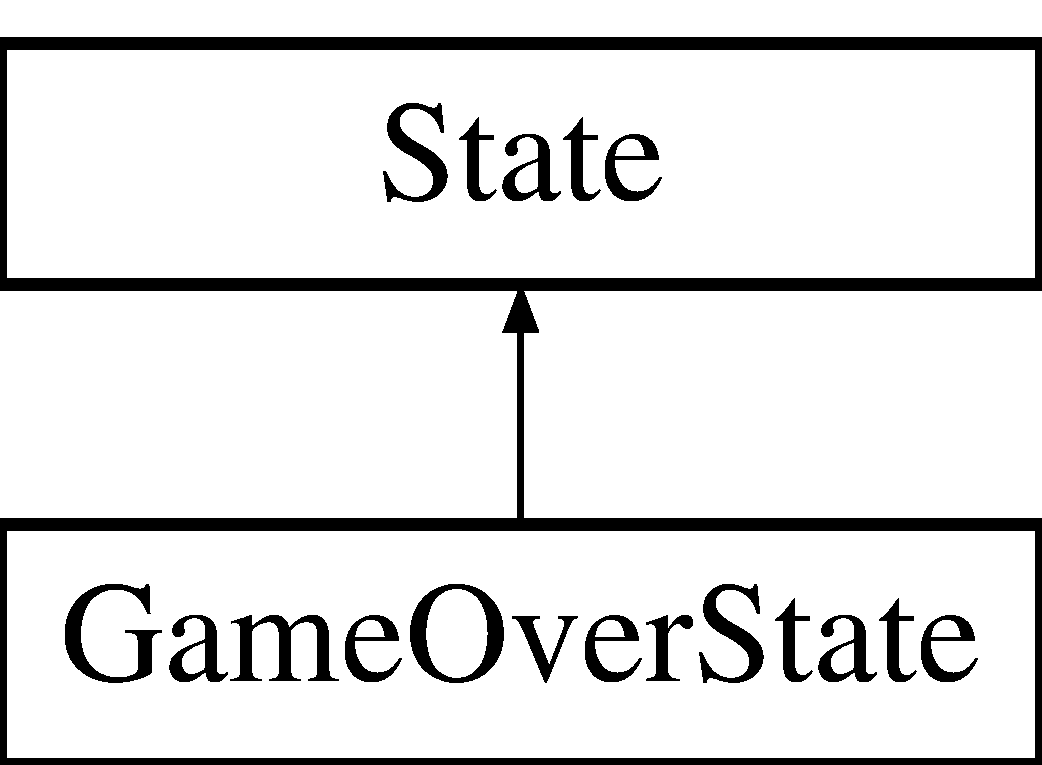
\includegraphics[height=2.000000cm]{classGameOverState}
\end{center}
\end{figure}
\subsection*{Métodos públicos}
\begin{DoxyCompactItemize}
\item 
\hypertarget{classGameOverState_ac57e844cdac39492f3b67e29e8ce7086}{}{\bfseries Game\+Over\+State} (\hyperlink{classStateStack}{State\+Stack} \&\hyperlink{classState_a86c8d3a5a1ee89896828be85a785fb04}{stack}, \hyperlink{classContext}{Context} $\ast$\hyperlink{classState_adc93e8ad3199b5891618ca88eed0436a}{context})\label{classGameOverState_ac57e844cdac39492f3b67e29e8ce7086}

\item 
virtual void \hyperlink{classGameOverState_a9decc1411647e390bfed0bdc009cd691}{draw} ()
\item 
virtual bool \hyperlink{classGameOverState_a8a2047b5c684965f33574b8aee7b7c8f}{update} (sf\+::\+Time dt)
\item 
virtual bool \hyperlink{classGameOverState_acf1dc2c7f58fe21b7cfababaf87ff20b}{handle\+Event} (const sf\+::\+Event \&event)
\item 
virtual void \hyperlink{classGameOverState_aa0e79a90d666351a0328b051dece3024}{pushed\+Action} ()
\end{DoxyCompactItemize}
\subsection*{Otros miembros heredados}


\subsection{Descripción detallada}
Estado de juego finalizado 

\subsection{Documentación de las funciones miembro}
\hypertarget{classGameOverState_a9decc1411647e390bfed0bdc009cd691}{}\index{Game\+Over\+State@{Game\+Over\+State}!draw@{draw}}
\index{draw@{draw}!Game\+Over\+State@{Game\+Over\+State}}
\subsubsection[{draw}]{\setlength{\rightskip}{0pt plus 5cm}void Game\+Over\+State\+::draw (
\begin{DoxyParamCaption}
{}
\end{DoxyParamCaption}
)\hspace{0.3cm}{\ttfamily [virtual]}}\label{classGameOverState_a9decc1411647e390bfed0bdc009cd691}
Dibuja el estado 

Implementa \hyperlink{classState_ae261605bc40b7e3959ce5df5457e4942}{State}.

\hypertarget{classGameOverState_acf1dc2c7f58fe21b7cfababaf87ff20b}{}\index{Game\+Over\+State@{Game\+Over\+State}!handle\+Event@{handle\+Event}}
\index{handle\+Event@{handle\+Event}!Game\+Over\+State@{Game\+Over\+State}}
\subsubsection[{handle\+Event}]{\setlength{\rightskip}{0pt plus 5cm}bool Game\+Over\+State\+::handle\+Event (
\begin{DoxyParamCaption}
\item[{const sf\+::\+Event \&}]{event}
\end{DoxyParamCaption}
)\hspace{0.3cm}{\ttfamily [virtual]}}\label{classGameOverState_acf1dc2c7f58fe21b7cfababaf87ff20b}
Procesa la entrada del usuario 
\begin{DoxyParams}{Parámetros}
{\em event} & evento \\
\hline
\end{DoxyParams}
\begin{DoxyReturn}{Devuelve}
true si lo ha procesado, false si no (o lo ha procesado pero que continúe) 
\end{DoxyReturn}


Implementa \hyperlink{classState_a19965f83460b248c42952aac8d001206}{State}.

\hypertarget{classGameOverState_aa0e79a90d666351a0328b051dece3024}{}\index{Game\+Over\+State@{Game\+Over\+State}!pushed\+Action@{pushed\+Action}}
\index{pushed\+Action@{pushed\+Action}!Game\+Over\+State@{Game\+Over\+State}}
\subsubsection[{pushed\+Action}]{\setlength{\rightskip}{0pt plus 5cm}void Game\+Over\+State\+::pushed\+Action (
\begin{DoxyParamCaption}
{}
\end{DoxyParamCaption}
)\hspace{0.3cm}{\ttfamily [virtual]}}\label{classGameOverState_aa0e79a90d666351a0328b051dece3024}
Método ejecutado cuando es puesto en pila 

Reimplementado de \hyperlink{classState_a3cc6a1378f32f9ed6a2d1d8140296808}{State}.

\hypertarget{classGameOverState_a8a2047b5c684965f33574b8aee7b7c8f}{}\index{Game\+Over\+State@{Game\+Over\+State}!update@{update}}
\index{update@{update}!Game\+Over\+State@{Game\+Over\+State}}
\subsubsection[{update}]{\setlength{\rightskip}{0pt plus 5cm}bool Game\+Over\+State\+::update (
\begin{DoxyParamCaption}
\item[{sf\+::\+Time}]{delta}
\end{DoxyParamCaption}
)\hspace{0.3cm}{\ttfamily [virtual]}}\label{classGameOverState_a8a2047b5c684965f33574b8aee7b7c8f}
Actualiza el estado 
\begin{DoxyParams}{Parámetros}
{\em delta} & tiempo entre frame y frame \\
\hline
\end{DoxyParams}
\begin{DoxyReturn}{Devuelve}
true si se ha actualizado 
\end{DoxyReturn}


Implementa \hyperlink{classState_aa6366828eb50639e86b94008cfad9c5d}{State}.



La documentación para esta clase fue generada a partir de los siguientes ficheros\+:\begin{DoxyCompactItemize}
\item 
Game\+Over\+State.\+h\item 
Game\+Over\+State.\+cpp\end{DoxyCompactItemize}

\hypertarget{classGameState}{}\section{Referencia de la Clase Game\+State}
\label{classGameState}\index{Game\+State@{Game\+State}}


{\ttfamily \#include $<$Game\+State.\+h$>$}

Diagrama de herencias de Game\+State\begin{figure}[H]
\begin{center}
\leavevmode
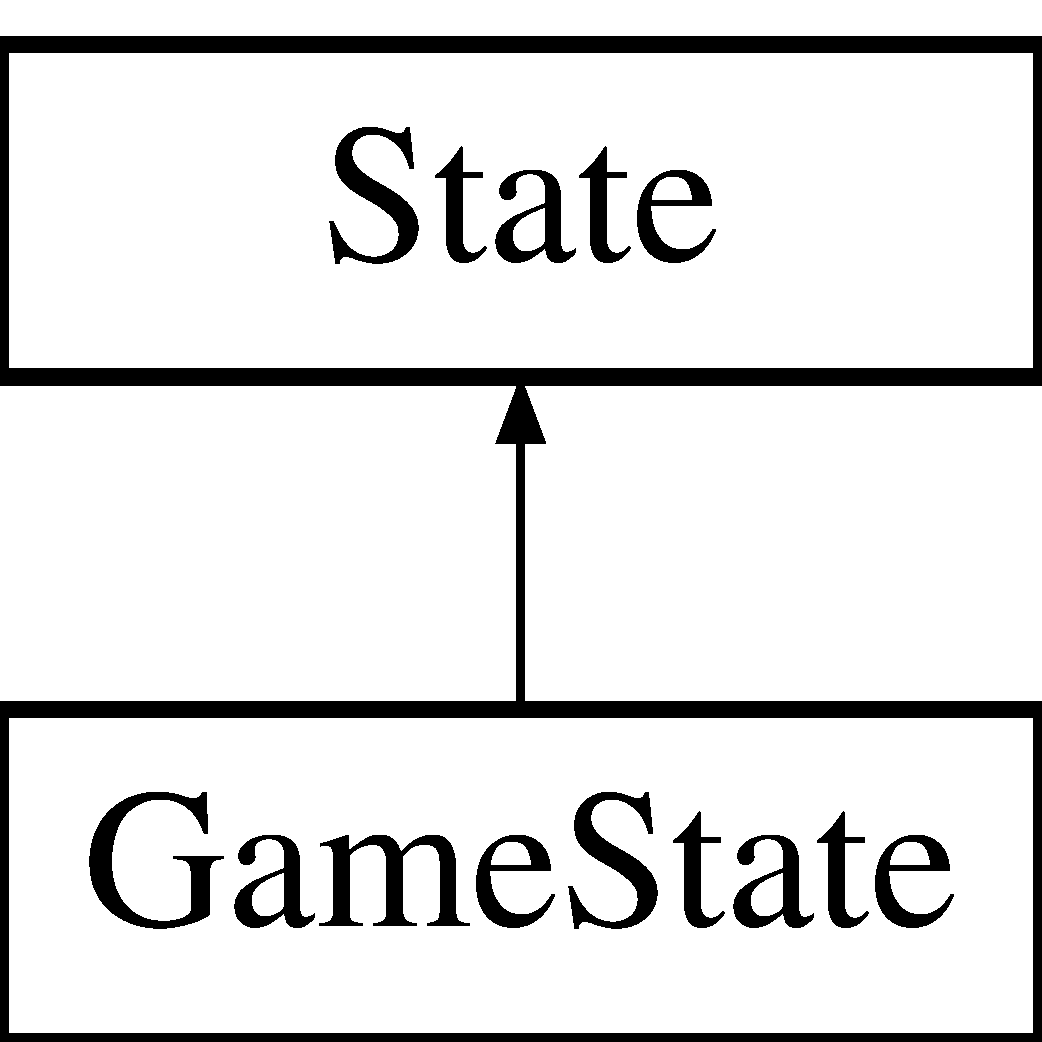
\includegraphics[height=2.000000cm]{classGameState}
\end{center}
\end{figure}
\subsection*{Métodos públicos}
\begin{DoxyCompactItemize}
\item 
\hypertarget{classGameState_ab88f7bafdb50469ca74512ad13b7cc66}{}{\bfseries Game\+State} (\hyperlink{classStateStack}{State\+Stack} \&\hyperlink{classState_a86c8d3a5a1ee89896828be85a785fb04}{stack}, \hyperlink{classContext}{Context} $\ast$\hyperlink{classState_adc93e8ad3199b5891618ca88eed0436a}{context})\label{classGameState_ab88f7bafdb50469ca74512ad13b7cc66}

\item 
virtual void \hyperlink{classGameState_a3c511417d8934943ae65c04681f321a3}{draw} ()
\item 
virtual bool \hyperlink{classGameState_a4ac988f0da5c33b43ff356890fcf9c1c}{update} (sf\+::\+Time dt)
\item 
virtual bool \hyperlink{classGameState_a000dd3306b1cb9faab5a86774a22aa6d}{handle\+Event} (const sf\+::\+Event \&event)
\item 
virtual void \hyperlink{classGameState_aaff561d6fe2a21a2084d093016a1d3be}{pushed\+Action} ()
\end{DoxyCompactItemize}
\subsection*{Otros miembros heredados}


\subsection{Descripción detallada}
Estado de juego 

\subsection{Documentación de las funciones miembro}
\hypertarget{classGameState_a3c511417d8934943ae65c04681f321a3}{}\index{Game\+State@{Game\+State}!draw@{draw}}
\index{draw@{draw}!Game\+State@{Game\+State}}
\subsubsection[{draw}]{\setlength{\rightskip}{0pt plus 5cm}void Game\+State\+::draw (
\begin{DoxyParamCaption}
{}
\end{DoxyParamCaption}
)\hspace{0.3cm}{\ttfamily [virtual]}}\label{classGameState_a3c511417d8934943ae65c04681f321a3}
Dibuja el estado 

Implementa \hyperlink{classState_ae261605bc40b7e3959ce5df5457e4942}{State}.

\hypertarget{classGameState_a000dd3306b1cb9faab5a86774a22aa6d}{}\index{Game\+State@{Game\+State}!handle\+Event@{handle\+Event}}
\index{handle\+Event@{handle\+Event}!Game\+State@{Game\+State}}
\subsubsection[{handle\+Event}]{\setlength{\rightskip}{0pt plus 5cm}bool Game\+State\+::handle\+Event (
\begin{DoxyParamCaption}
\item[{const sf\+::\+Event \&}]{event}
\end{DoxyParamCaption}
)\hspace{0.3cm}{\ttfamily [virtual]}}\label{classGameState_a000dd3306b1cb9faab5a86774a22aa6d}
Procesa la entrada del usuario 
\begin{DoxyParams}{Parámetros}
{\em event} & evento \\
\hline
\end{DoxyParams}
\begin{DoxyReturn}{Devuelve}
true si lo ha procesado, false si no (o lo ha procesado pero que continúe) 
\end{DoxyReturn}


Implementa \hyperlink{classState_a19965f83460b248c42952aac8d001206}{State}.

\hypertarget{classGameState_aaff561d6fe2a21a2084d093016a1d3be}{}\index{Game\+State@{Game\+State}!pushed\+Action@{pushed\+Action}}
\index{pushed\+Action@{pushed\+Action}!Game\+State@{Game\+State}}
\subsubsection[{pushed\+Action}]{\setlength{\rightskip}{0pt plus 5cm}void Game\+State\+::pushed\+Action (
\begin{DoxyParamCaption}
{}
\end{DoxyParamCaption}
)\hspace{0.3cm}{\ttfamily [virtual]}}\label{classGameState_aaff561d6fe2a21a2084d093016a1d3be}
Método ejecutado cuando es puesto en pila 

Reimplementado de \hyperlink{classState_a3cc6a1378f32f9ed6a2d1d8140296808}{State}.

\hypertarget{classGameState_a4ac988f0da5c33b43ff356890fcf9c1c}{}\index{Game\+State@{Game\+State}!update@{update}}
\index{update@{update}!Game\+State@{Game\+State}}
\subsubsection[{update}]{\setlength{\rightskip}{0pt plus 5cm}bool Game\+State\+::update (
\begin{DoxyParamCaption}
\item[{sf\+::\+Time}]{delta}
\end{DoxyParamCaption}
)\hspace{0.3cm}{\ttfamily [virtual]}}\label{classGameState_a4ac988f0da5c33b43ff356890fcf9c1c}
Actualiza el estado 
\begin{DoxyParams}{Parámetros}
{\em delta} & tiempo entre frame y frame \\
\hline
\end{DoxyParams}
\begin{DoxyReturn}{Devuelve}
true si se ha actualizado 
\end{DoxyReturn}


Implementa \hyperlink{classState_aa6366828eb50639e86b94008cfad9c5d}{State}.



La documentación para esta clase fue generada a partir de los siguientes ficheros\+:\begin{DoxyCompactItemize}
\item 
Game\+State.\+h\item 
Game\+State.\+cpp\end{DoxyCompactItemize}

\hypertarget{classHashIdEntity}{}\section{Referencia de la Clase Hash\+Id\+Entity}
\label{classHashIdEntity}\index{Hash\+Id\+Entity@{Hash\+Id\+Entity}}


{\ttfamily \#include $<$Hash\+Id\+Entity.\+h$>$}

\subsection*{Métodos públicos}
\begin{DoxyCompactItemize}
\item 
\hypertarget{classHashIdEntity_a157853f9e3cc6a44eeb5f323a6abd342}{}const std\+::size\+\_\+t {\bfseries operator()} (\hyperlink{classIdEntity}{Id\+Entity} const \&t) const \label{classHashIdEntity_a157853f9e3cc6a44eeb5f323a6abd342}

\end{DoxyCompactItemize}


\subsection{Descripción detallada}
Clase para el hasheo de \hyperlink{classIdEntity}{Id\+Entity} 
\begin{DoxyParams}{Parámetros}
{\em t} & id\+Entity a calcular \\
\hline
\end{DoxyParams}
\begin{DoxyReturn}{Devuelve}
hash calculado 
\end{DoxyReturn}


La documentación para esta clase fue generada a partir del siguiente fichero\+:\begin{DoxyCompactItemize}
\item 
Hash\+Id\+Entity.\+h\end{DoxyCompactItemize}

\hypertarget{classHole}{}\section{Referencia de la Clase Hole}
\label{classHole}\index{Hole@{Hole}}


{\ttfamily \#include $<$Hole.\+h$>$}

Diagrama de herencias de Hole\begin{figure}[H]
\begin{center}
\leavevmode
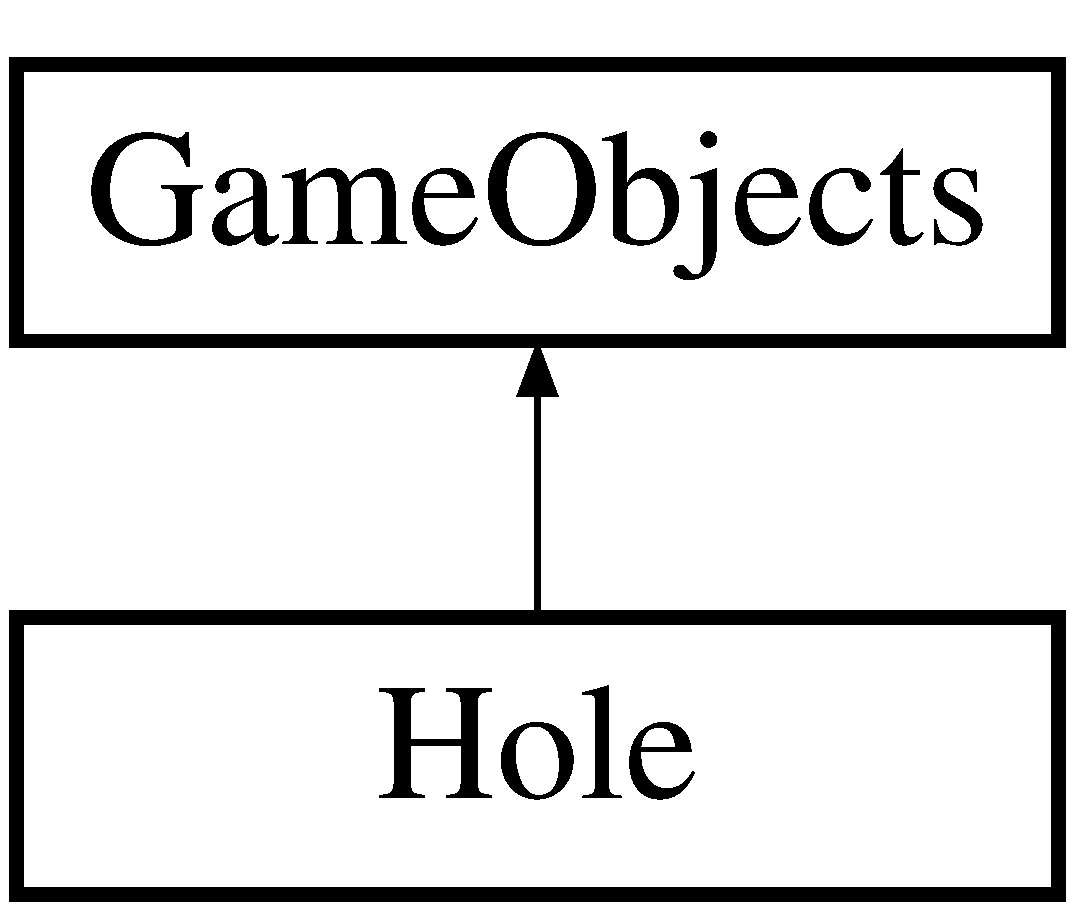
\includegraphics[height=2.000000cm]{classHole}
\end{center}
\end{figure}
\subsection*{Métodos públicos}
\begin{DoxyCompactItemize}
\item 
virtual \hyperlink{classEntity}{Entity} $\ast$ \hyperlink{classHole_a972b6c3658292ff3b8c78e1c7c1076e8}{prepare\+Entity} (\hyperlink{classPropertyManager}{Property\+Manager} \&parameters)
\end{DoxyCompactItemize}


\subsection{Descripción detallada}
Constructor de una entidad concreta, un objeto del juego define un agujero 

\subsection{Documentación de las funciones miembro}
\hypertarget{classHole_a972b6c3658292ff3b8c78e1c7c1076e8}{}\index{Hole@{Hole}!prepare\+Entity@{prepare\+Entity}}
\index{prepare\+Entity@{prepare\+Entity}!Hole@{Hole}}
\subsubsection[{prepare\+Entity}]{\setlength{\rightskip}{0pt plus 5cm}{\bf Entity} $\ast$ Hole\+::prepare\+Entity (
\begin{DoxyParamCaption}
\item[{{\bf Property\+Manager} \&}]{parameters}
\end{DoxyParamCaption}
)\hspace{0.3cm}{\ttfamily [virtual]}}\label{classHole_a972b6c3658292ff3b8c78e1c7c1076e8}
Devuelve una entidad que define un agujero dado unos parámetros 
\begin{DoxyParams}{Parámetros}
{\em parameters} & conjunto de parámetros \\
\hline
\end{DoxyParams}
\begin{DoxyReturn}{Devuelve}
entidad formada 
\end{DoxyReturn}


Implementa \hyperlink{classGameObjects_ad8d8177b229922b5a29e7355c8cf54ca}{Game\+Objects}.



La documentación para esta clase fue generada a partir de los siguientes ficheros\+:\begin{DoxyCompactItemize}
\item 
Hole.\+h\item 
Hole.\+cpp\end{DoxyCompactItemize}

\hypertarget{classIdEntity}{}\section{Referencia de la Clase Id\+Entity}
\label{classIdEntity}\index{Id\+Entity@{Id\+Entity}}


{\ttfamily \#include $<$Id\+Entity.\+h$>$}

\subsection*{Métodos públicos}
\begin{DoxyCompactItemize}
\item 
\hyperlink{classIdEntity_ae1d9bb5704ec03ec7b940e71fec68cd7}{Id\+Entity} (int id)
\item 
\hyperlink{classIdEntity_a4a8769f110d882e6a5954a7d242a9b8a}{Id\+Entity} ()
\item 
\hyperlink{classIdEntity_aed12ca9eb669e2f6fdd127a717b81d48}{Id\+Entity} (const \hyperlink{classIdEntity}{Id\+Entity} \&orig)
\item 
virtual \hyperlink{classIdEntity_a3d5a29e369f066892a8df8eb0b6a1695}{$\sim$\+Id\+Entity} ()
\item 
\hypertarget{classIdEntity_ad974b59e551e9021edfa791cc5cc378f}{}bool {\bfseries operator==} (const \hyperlink{classIdEntity}{Id\+Entity} lhs) const \label{classIdEntity_ad974b59e551e9021edfa791cc5cc378f}

\item 
\hypertarget{classIdEntity_a75cb74ff41413957f2a24efffa1ba374}{}bool {\bfseries operator!=} (const \hyperlink{classIdEntity}{Id\+Entity} \&lhs) const \label{classIdEntity_a75cb74ff41413957f2a24efffa1ba374}

\item 
\hypertarget{classIdEntity_ab096d00789f0654dfeec665e99df94dc}{}bool {\bfseries operator$<$} (const \hyperlink{classIdEntity}{Id\+Entity} \&lhs) const \label{classIdEntity_ab096d00789f0654dfeec665e99df94dc}

\item 
\hypertarget{classIdEntity_a0a2a93f6cd371edc28afa06f80d3ae6c}{}bool {\bfseries operator$>$} (const \hyperlink{classIdEntity}{Id\+Entity} \&lhs) const \label{classIdEntity_a0a2a93f6cd371edc28afa06f80d3ae6c}

\item 
\hypertarget{classIdEntity_a5161f71d20c4affc3c98d738b80f3dfd}{}bool {\bfseries operator$<$=} (const \hyperlink{classIdEntity}{Id\+Entity} \&lhs) const \label{classIdEntity_a5161f71d20c4affc3c98d738b80f3dfd}

\item 
\hypertarget{classIdEntity_af40f1b52b82ba155bbc8b8634eb07518}{}bool {\bfseries operator$>$=} (const \hyperlink{classIdEntity}{Id\+Entity} \&lhs) const \label{classIdEntity_af40f1b52b82ba155bbc8b8634eb07518}

\item 
\hypertarget{classIdEntity_a1b1312f974928ffb127f8f38b3784a27}{}int {\bfseries get\+Id} () const \label{classIdEntity_a1b1312f974928ffb127f8f38b3784a27}

\end{DoxyCompactItemize}


\subsection{Descripción detallada}
Identificador para una entidad 

\subsection{Documentación del constructor y destructor}
\hypertarget{classIdEntity_ae1d9bb5704ec03ec7b940e71fec68cd7}{}\index{Id\+Entity@{Id\+Entity}!Id\+Entity@{Id\+Entity}}
\index{Id\+Entity@{Id\+Entity}!Id\+Entity@{Id\+Entity}}
\subsubsection[{Id\+Entity}]{\setlength{\rightskip}{0pt plus 5cm}Id\+Entity\+::\+Id\+Entity (
\begin{DoxyParamCaption}
\item[{int}]{id}
\end{DoxyParamCaption}
)\hspace{0.3cm}{\ttfamily [inline]}}\label{classIdEntity_ae1d9bb5704ec03ec7b940e71fec68cd7}
Constructor 
\begin{DoxyParams}{Parámetros}
{\em id} & el id de la entidad \\
\hline
\end{DoxyParams}
\hypertarget{classIdEntity_a4a8769f110d882e6a5954a7d242a9b8a}{}\index{Id\+Entity@{Id\+Entity}!Id\+Entity@{Id\+Entity}}
\index{Id\+Entity@{Id\+Entity}!Id\+Entity@{Id\+Entity}}
\subsubsection[{Id\+Entity}]{\setlength{\rightskip}{0pt plus 5cm}Id\+Entity\+::\+Id\+Entity (
\begin{DoxyParamCaption}
{}
\end{DoxyParamCaption}
)\hspace{0.3cm}{\ttfamily [inline]}}\label{classIdEntity_a4a8769f110d882e6a5954a7d242a9b8a}
Constructor por defecto, se asigna un nuevo identificador no usado hasta el momento \hypertarget{classIdEntity_aed12ca9eb669e2f6fdd127a717b81d48}{}\index{Id\+Entity@{Id\+Entity}!Id\+Entity@{Id\+Entity}}
\index{Id\+Entity@{Id\+Entity}!Id\+Entity@{Id\+Entity}}
\subsubsection[{Id\+Entity}]{\setlength{\rightskip}{0pt plus 5cm}Id\+Entity\+::\+Id\+Entity (
\begin{DoxyParamCaption}
\item[{const {\bf Id\+Entity} \&}]{orig}
\end{DoxyParamCaption}
)\hspace{0.3cm}{\ttfamily [inline]}}\label{classIdEntity_aed12ca9eb669e2f6fdd127a717b81d48}
Constructor copia 
\begin{DoxyParams}{Parámetros}
{\em orig} & otro identificador \\
\hline
\end{DoxyParams}
\hypertarget{classIdEntity_a3d5a29e369f066892a8df8eb0b6a1695}{}\index{Id\+Entity@{Id\+Entity}!````~Id\+Entity@{$\sim$\+Id\+Entity}}
\index{````~Id\+Entity@{$\sim$\+Id\+Entity}!Id\+Entity@{Id\+Entity}}
\subsubsection[{$\sim$\+Id\+Entity}]{\setlength{\rightskip}{0pt plus 5cm}virtual Id\+Entity\+::$\sim$\+Id\+Entity (
\begin{DoxyParamCaption}
{}
\end{DoxyParamCaption}
)\hspace{0.3cm}{\ttfamily [inline]}, {\ttfamily [virtual]}}\label{classIdEntity_a3d5a29e369f066892a8df8eb0b6a1695}
Destructor 

La documentación para esta clase fue generada a partir del siguiente fichero\+:\begin{DoxyCompactItemize}
\item 
Id\+Entity.\+h\end{DoxyCompactItemize}

\hypertarget{structIEDGE}{}\section{Referencia de la Estructura I\+E\+D\+G\+E}
\label{structIEDGE}\index{I\+E\+D\+G\+E@{I\+E\+D\+G\+E}}
\subsection*{Campos de datos}
\begin{DoxyCompactItemize}
\item 
\hypertarget{structIEDGE_a38d2facfa290c17f417fb8c8375455e3}{}int {\bfseries p1}\label{structIEDGE_a38d2facfa290c17f417fb8c8375455e3}

\item 
\hypertarget{structIEDGE_a78aa0fc06147e253ae572ce7efc5be5a}{}int {\bfseries p2}\label{structIEDGE_a78aa0fc06147e253ae572ce7efc5be5a}

\end{DoxyCompactItemize}


La documentación para esta estructura fue generada a partir del siguiente fichero\+:\begin{DoxyCompactItemize}
\item 
Delaunay\+Triangulation.\+h\end{DoxyCompactItemize}

\hypertarget{classIProperty}{}\section{Referencia de la Clase I\+Property}
\label{classIProperty}\index{I\+Property@{I\+Property}}
Diagrama de herencias de I\+Property\begin{figure}[H]
\begin{center}
\leavevmode
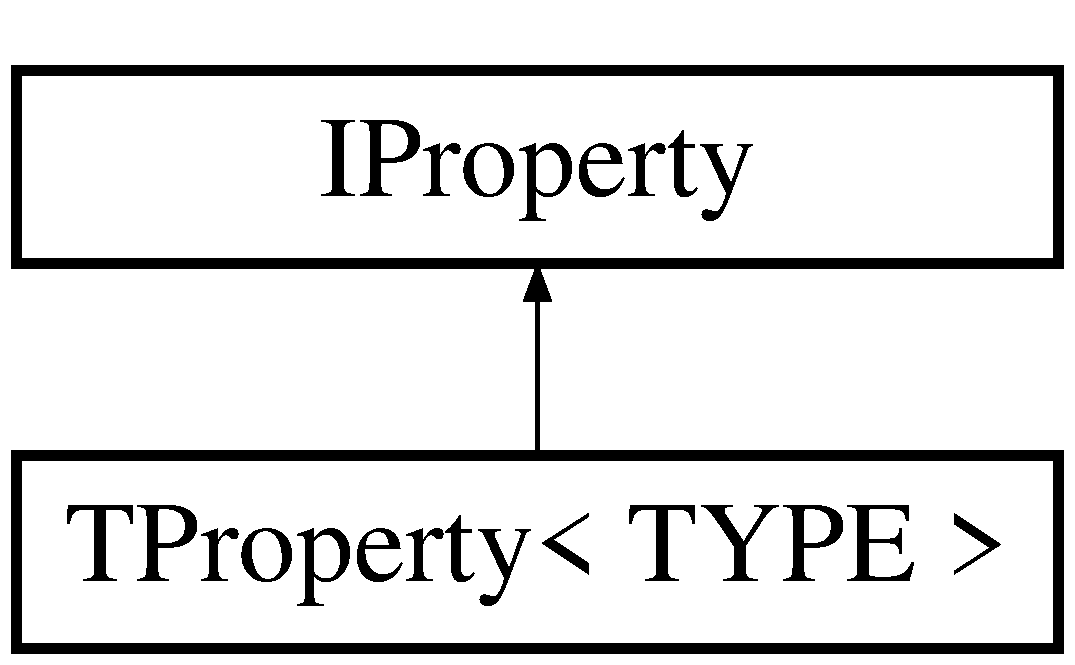
\includegraphics[height=2.000000cm]{classIProperty}
\end{center}
\end{figure}
\subsection*{Estructuras de datos}
\begin{DoxyCompactItemize}
\item 
class \hyperlink{classIProperty_1_1Type__t}{Type\+\_\+t}
\end{DoxyCompactItemize}
\subsection*{Métodos públicos}
\begin{DoxyCompactItemize}
\item 
\hyperlink{classIProperty_a8d7906c8be889ae2b85cd712071c59a9}{I\+Property} (std\+::string the\+Type, const std\+::string the\+Property\+I\+D)
\item 
virtual \hyperlink{classIProperty_a5f96ff700cd8e9cd86fd009a09b0448a}{$\sim$\+I\+Property} ()
\item 
\hyperlink{classIProperty_1_1Type__t}{Type\+\_\+t} $\ast$ \hyperlink{classIProperty_a1d7350322f5c32e8e67879a5e5475b50}{Get\+Type} (void)
\item 
const std\+::string \hyperlink{classIProperty_af96e4937115a87d7e116df5afbd0ca37}{Get\+I\+D} (void) const 
\item 
virtual void \hyperlink{classIProperty_af257f5c126fedd5ad89726cdeeccbc0a}{Update} ()=0
\item 
virtual \hyperlink{classIProperty}{I\+Property} $\ast$ \hyperlink{classIProperty_a5ae2b99d460cc149f4afa04e9d97d584}{Make\+Clone} ()=0
\end{DoxyCompactItemize}
\subsection*{Métodos protegidos}
\begin{DoxyCompactItemize}
\item 
void \hyperlink{classIProperty_a56dd22e54202123098eafedf52c22feb}{Set\+Type} (std\+::string the\+Type)
\end{DoxyCompactItemize}


\subsection{Documentación del constructor y destructor}
\hypertarget{classIProperty_a8d7906c8be889ae2b85cd712071c59a9}{}\index{I\+Property@{I\+Property}!I\+Property@{I\+Property}}
\index{I\+Property@{I\+Property}!I\+Property@{I\+Property}}
\subsubsection[{I\+Property}]{\setlength{\rightskip}{0pt plus 5cm}I\+Property\+::\+I\+Property (
\begin{DoxyParamCaption}
\item[{std\+::string}]{the\+Type, }
\item[{const std\+::string}]{the\+Property\+I\+D}
\end{DoxyParamCaption}
)}\label{classIProperty_a8d7906c8be889ae2b85cd712071c59a9}
\hyperlink{classIProperty}{I\+Property} default constructor 
\begin{DoxyParams}[1]{Parámetros}
\mbox{\tt in}  & {\em the\+Type} & of property this property represents \\
\hline
\mbox{\tt in}  & {\em the\+Property\+I\+D} & to use for this property \\
\hline
\end{DoxyParams}
\hypertarget{classIProperty_a5f96ff700cd8e9cd86fd009a09b0448a}{}\index{I\+Property@{I\+Property}!````~I\+Property@{$\sim$\+I\+Property}}
\index{````~I\+Property@{$\sim$\+I\+Property}!I\+Property@{I\+Property}}
\subsubsection[{$\sim$\+I\+Property}]{\setlength{\rightskip}{0pt plus 5cm}I\+Property\+::$\sim$\+I\+Property (
\begin{DoxyParamCaption}
{}
\end{DoxyParamCaption}
)\hspace{0.3cm}{\ttfamily [virtual]}}\label{classIProperty_a5f96ff700cd8e9cd86fd009a09b0448a}
\hyperlink{classIProperty}{I\+Property} destructor 

\subsection{Documentación de las funciones miembro}
\hypertarget{classIProperty_af96e4937115a87d7e116df5afbd0ca37}{}\index{I\+Property@{I\+Property}!Get\+I\+D@{Get\+I\+D}}
\index{Get\+I\+D@{Get\+I\+D}!I\+Property@{I\+Property}}
\subsubsection[{Get\+I\+D}]{\setlength{\rightskip}{0pt plus 5cm}const std\+::string I\+Property\+::\+Get\+I\+D (
\begin{DoxyParamCaption}
\item[{void}]{}
\end{DoxyParamCaption}
) const}\label{classIProperty_af96e4937115a87d7e116df5afbd0ca37}
Get\+I\+D will return the Property I\+D used for this property. \begin{DoxyReturn}{Devuelve}
the property I\+D for this property 
\end{DoxyReturn}
\hypertarget{classIProperty_a1d7350322f5c32e8e67879a5e5475b50}{}\index{I\+Property@{I\+Property}!Get\+Type@{Get\+Type}}
\index{Get\+Type@{Get\+Type}!I\+Property@{I\+Property}}
\subsubsection[{Get\+Type}]{\setlength{\rightskip}{0pt plus 5cm}{\bf I\+Property\+::\+Type\+\_\+t} $\ast$ I\+Property\+::\+Get\+Type (
\begin{DoxyParamCaption}
\item[{void}]{}
\end{DoxyParamCaption}
)}\label{classIProperty_a1d7350322f5c32e8e67879a5e5475b50}
Get\+Type will return the \hyperlink{classIProperty_1_1Type__t}{Type\+\_\+t} type for this property \begin{DoxyReturn}{Devuelve}
the \hyperlink{classIProperty_1_1Type__t}{Type\+\_\+t} class for this property 
\end{DoxyReturn}
\hypertarget{classIProperty_a5ae2b99d460cc149f4afa04e9d97d584}{}\index{I\+Property@{I\+Property}!Make\+Clone@{Make\+Clone}}
\index{Make\+Clone@{Make\+Clone}!I\+Property@{I\+Property}}
\subsubsection[{Make\+Clone}]{\setlength{\rightskip}{0pt plus 5cm}virtual {\bf I\+Property}$\ast$ I\+Property\+::\+Make\+Clone (
\begin{DoxyParamCaption}
{}
\end{DoxyParamCaption}
)\hspace{0.3cm}{\ttfamily [pure virtual]}}\label{classIProperty_a5ae2b99d460cc149f4afa04e9d97d584}
Make\+Clone is responsible for creating a clone of this \hyperlink{classIProperty}{I\+Property} derived class and returning it as part of the Prototype and Instance system. The value of the Property will also be copied into the clone. \begin{DoxyReturn}{Devuelve}
pointer to the \hyperlink{classIProperty}{I\+Property} derived class clone that was created 
\end{DoxyReturn}


Implementado en \hyperlink{classTProperty_a40e392d305cc3886255946359977edcb}{T\+Property$<$ T\+Y\+P\+E $>$}.

\hypertarget{classIProperty_a56dd22e54202123098eafedf52c22feb}{}\index{I\+Property@{I\+Property}!Set\+Type@{Set\+Type}}
\index{Set\+Type@{Set\+Type}!I\+Property@{I\+Property}}
\subsubsection[{Set\+Type}]{\setlength{\rightskip}{0pt plus 5cm}void I\+Property\+::\+Set\+Type (
\begin{DoxyParamCaption}
\item[{std\+::string}]{the\+Type}
\end{DoxyParamCaption}
)\hspace{0.3cm}{\ttfamily [protected]}}\label{classIProperty_a56dd22e54202123098eafedf52c22feb}
Set\+Type is responsible for setting the type of class this \hyperlink{classIProperty}{I\+Property} class represents and is usually called by the \hyperlink{classIProperty}{I\+Property} derived class to set the\+Type. 
\begin{DoxyParams}[1]{Parámetros}
\mbox{\tt in}  & {\em the\+Type} & to set for this \hyperlink{classIProperty}{I\+Property} derived class \\
\hline
\end{DoxyParams}
\hypertarget{classIProperty_af257f5c126fedd5ad89726cdeeccbc0a}{}\index{I\+Property@{I\+Property}!Update@{Update}}
\index{Update@{Update}!I\+Property@{I\+Property}}
\subsubsection[{Update}]{\setlength{\rightskip}{0pt plus 5cm}virtual void I\+Property\+::\+Update (
\begin{DoxyParamCaption}
{}
\end{DoxyParamCaption}
)\hspace{0.3cm}{\ttfamily [pure virtual]}}\label{classIProperty_af257f5c126fedd5ad89726cdeeccbc0a}
Update will be called for each \hyperlink{classIProperty}{I\+Property} registered with I\+Entity and enable each \hyperlink{classIProperty}{I\+Property} derived class to perform Update related tasks (e.\+g. frame counter, timer update, decreate in shields, etc). 

Implementado en \hyperlink{classTProperty_ab463fc86cb27252b763b38be21e82c3f}{T\+Property$<$ T\+Y\+P\+E $>$}.



La documentación para esta clase fue generada a partir de los siguientes ficheros\+:\begin{DoxyCompactItemize}
\item 
I\+Property.\+h\item 
I\+Property.\+cpp\end{DoxyCompactItemize}

\hypertarget{classISystem}{}\section{Referencia de la Clase I\+System}
\label{classISystem}\index{I\+System@{I\+System}}


{\ttfamily \#include $<$I\+System.\+h$>$}

Diagrama de herencias de I\+System\begin{figure}[H]
\begin{center}
\leavevmode
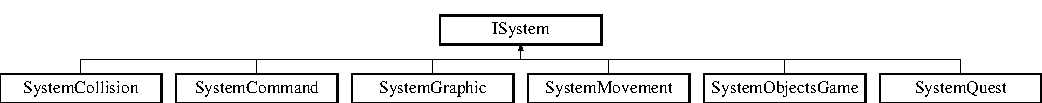
\includegraphics[height=1.382716cm]{classISystem}
\end{center}
\end{figure}
\subsection*{Métodos públicos}
\begin{DoxyCompactItemize}
\item 
Type\+System \hyperlink{classISystem_a6e94810e4a308aa6ae5ed03411a86800}{get\+Type} ()
\item 
virtual void \hyperlink{classISystem_ac9b257acd7d03dbd7aab149792ff98af}{initialize} ()
\item 
virtual void \hyperlink{classISystem_a4cc1cac06100c45d260a23d24d5618d6}{finalize} ()
\item 
virtual void \hyperlink{classISystem_a6931efd2517fd0c81237beeb04297421}{update} (sf\+::\+Time dt)
\item 
virtual void \hyperlink{classISystem_aef2545bd6ffac18186b566e4d3d2804b}{update\+Second\+Part} (sf\+::\+Time dt)
\item 
virtual void \hyperlink{classISystem_aaaef32b093b566b0573cb23e00f8c7ae}{register\+Entity} (\hyperlink{classEntity}{Entity} $\ast$entity)=0
\item 
virtual void \hyperlink{classISystem_a0e966d506838cfe09543ad4ccafa4998}{removed\+Entity} (\hyperlink{classEntity}{Entity} $\ast$entity)=0
\item 
bool \hyperlink{classISystem_ad5471c17b45154b31063a1ecbce4eeaa}{is\+Finalized} () const 
\item 
bool \hyperlink{classISystem_a6c075151dc75d7ee731947849b35f1d6}{is\+Initialized} () const 
\end{DoxyCompactItemize}
\subsection*{Atributos protegidos}
\begin{DoxyCompactItemize}
\item 
Type\+System \hyperlink{classISystem_ae9154cb0a7d9560f0bfa9169a384a995}{type}
\end{DoxyCompactItemize}


\subsection{Descripción detallada}
Clase base de un sistema 

\subsection{Documentación de las funciones miembro}
\hypertarget{classISystem_a4cc1cac06100c45d260a23d24d5618d6}{}\index{I\+System@{I\+System}!finalize@{finalize}}
\index{finalize@{finalize}!I\+System@{I\+System}}
\subsubsection[{finalize}]{\setlength{\rightskip}{0pt plus 5cm}virtual void I\+System\+::finalize (
\begin{DoxyParamCaption}
{}
\end{DoxyParamCaption}
)\hspace{0.3cm}{\ttfamily [inline]}, {\ttfamily [virtual]}}\label{classISystem_a4cc1cac06100c45d260a23d24d5618d6}
Finaliza el sistema 

Reimplementado en \hyperlink{classSystemGraphic_af59c303890f7faf14db27ab746a23d3a}{System\+Graphic}, \hyperlink{classSystemCollision_a8c8ae9c8bb8f9f69e4b656c4ff496a30}{System\+Collision}, \hyperlink{classSystemObjectsGame_a4357e0e5d2e42a6b3e80362cbfdbda39}{System\+Objects\+Game}, \hyperlink{classSystemQuest_a3c9f834570acf2277d4620e3ba16992d}{System\+Quest}, \hyperlink{classSystemCommand_ac9f9019b5d0facf91ed77815d6c577a7}{System\+Command} y \hyperlink{classSystemMovement_a2e4df7be9f17a4572116649552c9d073}{System\+Movement}.

\hypertarget{classISystem_a6e94810e4a308aa6ae5ed03411a86800}{}\index{I\+System@{I\+System}!get\+Type@{get\+Type}}
\index{get\+Type@{get\+Type}!I\+System@{I\+System}}
\subsubsection[{get\+Type}]{\setlength{\rightskip}{0pt plus 5cm}Type\+System I\+System\+::get\+Type (
\begin{DoxyParamCaption}
{}
\end{DoxyParamCaption}
)\hspace{0.3cm}{\ttfamily [inline]}}\label{classISystem_a6e94810e4a308aa6ae5ed03411a86800}
Devuelve el tipo del sistema \begin{DoxyReturn}{Devuelve}

\end{DoxyReturn}
\hypertarget{classISystem_ac9b257acd7d03dbd7aab149792ff98af}{}\index{I\+System@{I\+System}!initialize@{initialize}}
\index{initialize@{initialize}!I\+System@{I\+System}}
\subsubsection[{initialize}]{\setlength{\rightskip}{0pt plus 5cm}virtual void I\+System\+::initialize (
\begin{DoxyParamCaption}
{}
\end{DoxyParamCaption}
)\hspace{0.3cm}{\ttfamily [inline]}, {\ttfamily [virtual]}}\label{classISystem_ac9b257acd7d03dbd7aab149792ff98af}
Inicializa el sistema 

Reimplementado en \hyperlink{classSystemGraphic_a792331587037bbf7fdfdd487cd45575a}{System\+Graphic}, \hyperlink{classSystemCollision_ab2ced8fd115cd326a29a3535ddba7367}{System\+Collision}, \hyperlink{classSystemObjectsGame_a1d915c3471432c344a58af523085b87f}{System\+Objects\+Game}, \hyperlink{classSystemQuest_a48773430521559d0b5eaa931b53d8892}{System\+Quest}, \hyperlink{classSystemCommand_a4e1ca3703de37a8c187618d17a4a676e}{System\+Command} y \hyperlink{classSystemMovement_a5657b5507fd4f6a7bf92e9a9929881d3}{System\+Movement}.

\hypertarget{classISystem_ad5471c17b45154b31063a1ecbce4eeaa}{}\index{I\+System@{I\+System}!is\+Finalized@{is\+Finalized}}
\index{is\+Finalized@{is\+Finalized}!I\+System@{I\+System}}
\subsubsection[{is\+Finalized}]{\setlength{\rightskip}{0pt plus 5cm}bool I\+System\+::is\+Finalized (
\begin{DoxyParamCaption}
{}
\end{DoxyParamCaption}
) const\hspace{0.3cm}{\ttfamily [inline]}}\label{classISystem_ad5471c17b45154b31063a1ecbce4eeaa}
Devuele si el sistema ya finalizó \begin{DoxyReturn}{Devuelve}
true si ha finalizado 
\end{DoxyReturn}
\hypertarget{classISystem_a6c075151dc75d7ee731947849b35f1d6}{}\index{I\+System@{I\+System}!is\+Initialized@{is\+Initialized}}
\index{is\+Initialized@{is\+Initialized}!I\+System@{I\+System}}
\subsubsection[{is\+Initialized}]{\setlength{\rightskip}{0pt plus 5cm}bool I\+System\+::is\+Initialized (
\begin{DoxyParamCaption}
{}
\end{DoxyParamCaption}
) const\hspace{0.3cm}{\ttfamily [inline]}}\label{classISystem_a6c075151dc75d7ee731947849b35f1d6}
Devuelve si el sistema ya está inicializado \begin{DoxyReturn}{Devuelve}
true si está inicializado 
\end{DoxyReturn}
\hypertarget{classISystem_aaaef32b093b566b0573cb23e00f8c7ae}{}\index{I\+System@{I\+System}!register\+Entity@{register\+Entity}}
\index{register\+Entity@{register\+Entity}!I\+System@{I\+System}}
\subsubsection[{register\+Entity}]{\setlength{\rightskip}{0pt plus 5cm}virtual void I\+System\+::register\+Entity (
\begin{DoxyParamCaption}
\item[{{\bf Entity} $\ast$}]{entity}
\end{DoxyParamCaption}
)\hspace{0.3cm}{\ttfamily [pure virtual]}}\label{classISystem_aaaef32b093b566b0573cb23e00f8c7ae}
Registra una entidad en el sistema si es de su incumbencia 
\begin{DoxyParams}{Parámetros}
{\em entity} & entidad a registrar \\
\hline
\end{DoxyParams}


Implementado en \hyperlink{classSystemGraphic_a7b905fc340431b0521b975d82ef2fa45}{System\+Graphic}, \hyperlink{classSystemCollision_a228a39b4c9bc3d6b7934a25814acda7a}{System\+Collision}, \hyperlink{classSystemObjectsGame_a6d8cbcab3b14a4ddc4c45ebe0c7aed07}{System\+Objects\+Game}, \hyperlink{classSystemCommand_a6c00eed8d1b14f8f27bd5fb27ffcaffe}{System\+Command}, \hyperlink{classSystemMovement_ae7a01c74fcd8cfae49488a707cf32902}{System\+Movement} y \hyperlink{classSystemQuest_a03ce5db7875898ebae8c9424c1888c37}{System\+Quest}.

\hypertarget{classISystem_a0e966d506838cfe09543ad4ccafa4998}{}\index{I\+System@{I\+System}!removed\+Entity@{removed\+Entity}}
\index{removed\+Entity@{removed\+Entity}!I\+System@{I\+System}}
\subsubsection[{removed\+Entity}]{\setlength{\rightskip}{0pt plus 5cm}virtual void I\+System\+::removed\+Entity (
\begin{DoxyParamCaption}
\item[{{\bf Entity} $\ast$}]{entity}
\end{DoxyParamCaption}
)\hspace{0.3cm}{\ttfamily [pure virtual]}}\label{classISystem_a0e966d506838cfe09543ad4ccafa4998}
Elimina la entidad del sistema 
\begin{DoxyParams}{Parámetros}
{\em entity} & \\
\hline
\end{DoxyParams}


Implementado en \hyperlink{classSystemGraphic_a9dba6a98242f2c5f07bd52301bc3dacb}{System\+Graphic}, \hyperlink{classSystemCollision_a8890b0a585ac5e9a99510839a9713de4}{System\+Collision}, \hyperlink{classSystemObjectsGame_ae716ba020dded37eb7cc01e3dab32a1a}{System\+Objects\+Game}, \hyperlink{classSystemCommand_afde58b2c3b053a944dfa262da10eeea2}{System\+Command}, \hyperlink{classSystemMovement_a7fe2e159ce9ef32f5710d9a957a2450b}{System\+Movement} y \hyperlink{classSystemQuest_a588e9982c16288af4675b67bf9177080}{System\+Quest}.

\hypertarget{classISystem_a6931efd2517fd0c81237beeb04297421}{}\index{I\+System@{I\+System}!update@{update}}
\index{update@{update}!I\+System@{I\+System}}
\subsubsection[{update}]{\setlength{\rightskip}{0pt plus 5cm}virtual void I\+System\+::update (
\begin{DoxyParamCaption}
\item[{sf\+::\+Time}]{dt}
\end{DoxyParamCaption}
)\hspace{0.3cm}{\ttfamily [inline]}, {\ttfamily [virtual]}}\label{classISystem_a6931efd2517fd0c81237beeb04297421}
Actualiza el sistema en una primera tanda 
\begin{DoxyParams}{Parámetros}
{\em dt} & tiempo entre frame y frame \\
\hline
\end{DoxyParams}


Reimplementado en \hyperlink{classSystemObjectsGame_a6836f71bd70b620d8b86b98e6e3ee44b}{System\+Objects\+Game}, \hyperlink{classSystemGraphic_aaabd7eb4e9ce5d82dd39126239818283}{System\+Graphic}, \hyperlink{classSystemCollision_ab2dae21a0636bf6d24c6fd7f596f07d1}{System\+Collision}, \hyperlink{classSystemQuest_a76892fc5b11bdb7132e7499e46eb7977}{System\+Quest}, \hyperlink{classSystemCommand_a111fbabb149f7f59a6084a459dd5f37d}{System\+Command} y \hyperlink{classSystemMovement_aab4a789b0bf9d329461896e12ada82c4}{System\+Movement}.

\hypertarget{classISystem_aef2545bd6ffac18186b566e4d3d2804b}{}\index{I\+System@{I\+System}!update\+Second\+Part@{update\+Second\+Part}}
\index{update\+Second\+Part@{update\+Second\+Part}!I\+System@{I\+System}}
\subsubsection[{update\+Second\+Part}]{\setlength{\rightskip}{0pt plus 5cm}virtual void I\+System\+::update\+Second\+Part (
\begin{DoxyParamCaption}
\item[{sf\+::\+Time}]{dt}
\end{DoxyParamCaption}
)\hspace{0.3cm}{\ttfamily [inline]}, {\ttfamily [virtual]}}\label{classISystem_aef2545bd6ffac18186b566e4d3d2804b}
Actualiza el sistema en una segunda tanda 
\begin{DoxyParams}{Parámetros}
{\em dt} & tiempo entre frame y frame \\
\hline
\end{DoxyParams}


Reimplementado en \hyperlink{classSystemObjectsGame_ad238ad4e70fb3cc2a5648a7176e69233}{System\+Objects\+Game}, \hyperlink{classSystemGraphic_a0d46ab172987eed86b45ae016240034e}{System\+Graphic}, \hyperlink{classSystemCollision_a731cd70ffedfa221454348ad975ee82c}{System\+Collision}, \hyperlink{classSystemQuest_a3069bdc81a590c47c4479b63add3fc3d}{System\+Quest}, \hyperlink{classSystemCommand_a0ff2e49835ef779e59f04c56fcc87ee1}{System\+Command} y \hyperlink{classSystemMovement_afd66e76ecd00084594be9334434a689d}{System\+Movement}.



\subsection{Documentación de los campos}
\hypertarget{classISystem_ae9154cb0a7d9560f0bfa9169a384a995}{}\index{I\+System@{I\+System}!type@{type}}
\index{type@{type}!I\+System@{I\+System}}
\subsubsection[{type}]{\setlength{\rightskip}{0pt plus 5cm}Type\+System I\+System\+::type\hspace{0.3cm}{\ttfamily [protected]}}\label{classISystem_ae9154cb0a7d9560f0bfa9169a384a995}
Tipo del sistema 

La documentación para esta clase fue generada a partir de los siguientes ficheros\+:\begin{DoxyCompactItemize}
\item 
I\+System.\+h\item 
I\+System.\+cpp\end{DoxyCompactItemize}

\hypertarget{structITRIANGLE}{}\section{Referencia de la Estructura I\+T\+R\+I\+A\+N\+G\+L\+E}
\label{structITRIANGLE}\index{I\+T\+R\+I\+A\+N\+G\+L\+E@{I\+T\+R\+I\+A\+N\+G\+L\+E}}


{\ttfamily \#include $<$Delaunay\+Triangulation.\+h$>$}

\subsection*{Campos de datos}
\begin{DoxyCompactItemize}
\item 
\hypertarget{structITRIANGLE_aa1e37637bc334917eebe0ebe876a1a7f}{}int {\bfseries p1}\label{structITRIANGLE_aa1e37637bc334917eebe0ebe876a1a7f}

\item 
\hypertarget{structITRIANGLE_a93d3170df8fd638bbefe05f86716bd98}{}int {\bfseries p2}\label{structITRIANGLE_a93d3170df8fd638bbefe05f86716bd98}

\item 
\hypertarget{structITRIANGLE_ae949f00b13e5ed72d47ee773ad4ce5b4}{}int {\bfseries p3}\label{structITRIANGLE_ae949f00b13e5ed72d47ee773ad4ce5b4}

\end{DoxyCompactItemize}


\subsection{Descripción detallada}
Estructuras para la triangulación 

La documentación para esta estructura fue generada a partir del siguiente fichero\+:\begin{DoxyCompactItemize}
\item 
Delaunay\+Triangulation.\+h\end{DoxyCompactItemize}

\hypertarget{classIXMLParser}{}\section{Referencia de la Clase I\+X\+M\+L\+Parser}
\label{classIXMLParser}\index{I\+X\+M\+L\+Parser@{I\+X\+M\+L\+Parser}}


{\ttfamily \#include $<$I\+X\+M\+L\+Parser.\+h$>$}

Diagrama de herencias de I\+X\+M\+L\+Parser\begin{figure}[H]
\begin{center}
\leavevmode
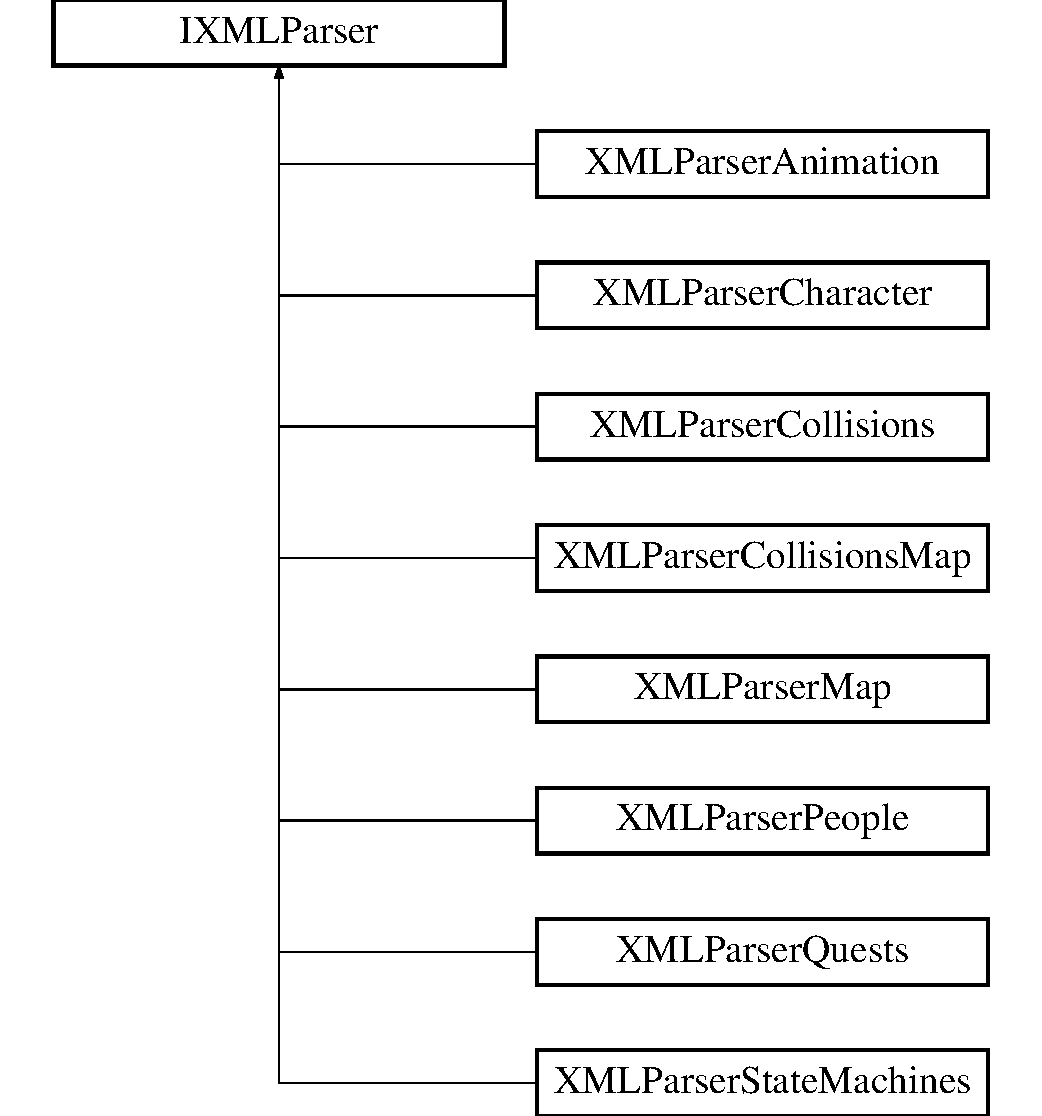
\includegraphics[height=9.000000cm]{classIXMLParser}
\end{center}
\end{figure}
\subsection*{Métodos públicos}
\begin{DoxyCompactItemize}
\item 
void \hyperlink{classIXMLParser_afe97ecb6c26a8d2c7d91ede1265b924d}{set\+X\+M\+L} (tinyxml2\+::\+X\+M\+L\+Document \&path)
\item 
void \hyperlink{classIXMLParser_a4e8bacc2f7ed0c13117e8e701cc5b9e4}{set\+X\+M\+L} (\hyperlink{classXMLDocument}{X\+M\+L\+Document} \&path)
\item 
void \hyperlink{classIXMLParser_a9ff44f69f9c9f995259514deb9e279e5}{set\+Resources} (\hyperlink{classResourceHolder}{Resource\+Holder}$<$ std\+::string, sf\+::\+Texture $>$ $\ast$\hyperlink{classIXMLParser_af05edc520158df67ae6417b626a09407}{textures})
\item 
virtual void \hyperlink{classIXMLParser_a2d6e54d4628bdf52a45ac1e18902b3d3}{parse} (\hyperlink{unionDataUnion}{Data\+Union} \&data)=0
\end{DoxyCompactItemize}
\subsection*{Métodos públicos estáticos}
\begin{DoxyCompactItemize}
\item 
static \hyperlink{classIXMLParser}{I\+X\+M\+L\+Parser} $\ast$ \hyperlink{classIXMLParser_acbf34ba27a24dc449e8303194df4f2a2}{make\+\_\+parser} (Type\+Parser choice)
\end{DoxyCompactItemize}
\subsection*{Atributos protegidos}
\begin{DoxyCompactItemize}
\item 
tinyxml2\+::\+X\+M\+L\+Document $\ast$ \hyperlink{classIXMLParser_a8a83507efb159b3eadbb5302d97c0d6a}{doc}
\item 
\hyperlink{classResourceHolder}{Resource\+Holder}$<$ std\+::string, sf\+::\+Texture $>$ $\ast$ \hyperlink{classIXMLParser_af05edc520158df67ae6417b626a09407}{textures}
\end{DoxyCompactItemize}


\subsection{Descripción detallada}
Clase base para un parseador de xml 

\subsection{Documentación de las funciones miembro}
\hypertarget{classIXMLParser_acbf34ba27a24dc449e8303194df4f2a2}{}\index{I\+X\+M\+L\+Parser@{I\+X\+M\+L\+Parser}!make\+\_\+parser@{make\+\_\+parser}}
\index{make\+\_\+parser@{make\+\_\+parser}!I\+X\+M\+L\+Parser@{I\+X\+M\+L\+Parser}}
\subsubsection[{make\+\_\+parser}]{\setlength{\rightskip}{0pt plus 5cm}{\bf I\+X\+M\+L\+Parser} $\ast$ I\+X\+M\+L\+Parser\+::make\+\_\+parser (
\begin{DoxyParamCaption}
\item[{Type\+Parser}]{choice}
\end{DoxyParamCaption}
)\hspace{0.3cm}{\ttfamily [static]}}\label{classIXMLParser_acbf34ba27a24dc449e8303194df4f2a2}
Devuelve el parseador concreto al tipo escogido 
\begin{DoxyParams}{Parámetros}
{\em choice} & tipo de parseador requerido \\
\hline
\end{DoxyParams}
\begin{DoxyReturn}{Devuelve}
parseador pedido 
\end{DoxyReturn}
\hypertarget{classIXMLParser_a2d6e54d4628bdf52a45ac1e18902b3d3}{}\index{I\+X\+M\+L\+Parser@{I\+X\+M\+L\+Parser}!parse@{parse}}
\index{parse@{parse}!I\+X\+M\+L\+Parser@{I\+X\+M\+L\+Parser}}
\subsubsection[{parse}]{\setlength{\rightskip}{0pt plus 5cm}virtual void I\+X\+M\+L\+Parser\+::parse (
\begin{DoxyParamCaption}
\item[{{\bf Data\+Union} \&}]{data}
\end{DoxyParamCaption}
)\hspace{0.3cm}{\ttfamily [pure virtual]}}\label{classIXMLParser_a2d6e54d4628bdf52a45ac1e18902b3d3}
Parsea los datos 
\begin{DoxyParams}{Parámetros}
{\em data} & \\
\hline
\end{DoxyParams}


Implementado en \hyperlink{classXMLParserCollisionsMap_a2cd272aef88a40c0f649d13b7821e118}{X\+M\+L\+Parser\+Collisions\+Map}, \hyperlink{classXMLParserCollisions_ae22d366d5d11adba7e89f3a183160988}{X\+M\+L\+Parser\+Collisions}, \hyperlink{classXMLParserMap_a428974998d952d3d8a84db0b02176765}{X\+M\+L\+Parser\+Map}, \hyperlink{classXMLParserCharacter_af8caeb3dc23d4b4f3b726824e0220782}{X\+M\+L\+Parser\+Character}, \hyperlink{classXMLParserPeople_a42f23e662f772245febe910aeee07ce3}{X\+M\+L\+Parser\+People}, \hyperlink{classXMLParserQuests_a533240568f62cd15fedf6c32bcb50cf4}{X\+M\+L\+Parser\+Quests}, \hyperlink{classXMLParserAnimation_a9b10d45d037d28b4c4849ef3217a7603}{X\+M\+L\+Parser\+Animation} y \hyperlink{classXMLParserStateMachines_a7af4decc72879799aa43260418bb021b}{X\+M\+L\+Parser\+State\+Machines}.

\hypertarget{classIXMLParser_a9ff44f69f9c9f995259514deb9e279e5}{}\index{I\+X\+M\+L\+Parser@{I\+X\+M\+L\+Parser}!set\+Resources@{set\+Resources}}
\index{set\+Resources@{set\+Resources}!I\+X\+M\+L\+Parser@{I\+X\+M\+L\+Parser}}
\subsubsection[{set\+Resources}]{\setlength{\rightskip}{0pt plus 5cm}void I\+X\+M\+L\+Parser\+::set\+Resources (
\begin{DoxyParamCaption}
\item[{{\bf Resource\+Holder}$<$ std\+::string, sf\+::\+Texture $>$ $\ast$}]{textures}
\end{DoxyParamCaption}
)}\label{classIXMLParser_a9ff44f69f9c9f995259514deb9e279e5}
Setea los recursos de imágenes que puede necesitar el parseador 
\begin{DoxyParams}{Parámetros}
{\em textures} & imagenes \\
\hline
\end{DoxyParams}
\hypertarget{classIXMLParser_afe97ecb6c26a8d2c7d91ede1265b924d}{}\index{I\+X\+M\+L\+Parser@{I\+X\+M\+L\+Parser}!set\+X\+M\+L@{set\+X\+M\+L}}
\index{set\+X\+M\+L@{set\+X\+M\+L}!I\+X\+M\+L\+Parser@{I\+X\+M\+L\+Parser}}
\subsubsection[{set\+X\+M\+L}]{\setlength{\rightskip}{0pt plus 5cm}void I\+X\+M\+L\+Parser\+::set\+X\+M\+L (
\begin{DoxyParamCaption}
\item[{tinyxml2\+::\+X\+M\+L\+Document \&}]{path}
\end{DoxyParamCaption}
)}\label{classIXMLParser_afe97ecb6c26a8d2c7d91ede1265b924d}
Setea el xml que parseará 
\begin{DoxyParams}{Parámetros}
{\em path} & documento xml a parsear \\
\hline
\end{DoxyParams}
\hypertarget{classIXMLParser_a4e8bacc2f7ed0c13117e8e701cc5b9e4}{}\index{I\+X\+M\+L\+Parser@{I\+X\+M\+L\+Parser}!set\+X\+M\+L@{set\+X\+M\+L}}
\index{set\+X\+M\+L@{set\+X\+M\+L}!I\+X\+M\+L\+Parser@{I\+X\+M\+L\+Parser}}
\subsubsection[{set\+X\+M\+L}]{\setlength{\rightskip}{0pt plus 5cm}void I\+X\+M\+L\+Parser\+::set\+X\+M\+L (
\begin{DoxyParamCaption}
\item[{{\bf X\+M\+L\+Document} \&}]{path}
\end{DoxyParamCaption}
)}\label{classIXMLParser_a4e8bacc2f7ed0c13117e8e701cc5b9e4}
Setea el xml que parseará 
\begin{DoxyParams}{Parámetros}
{\em path} & documento a parsear \\
\hline
\end{DoxyParams}


\subsection{Documentación de los campos}
\hypertarget{classIXMLParser_a8a83507efb159b3eadbb5302d97c0d6a}{}\index{I\+X\+M\+L\+Parser@{I\+X\+M\+L\+Parser}!doc@{doc}}
\index{doc@{doc}!I\+X\+M\+L\+Parser@{I\+X\+M\+L\+Parser}}
\subsubsection[{doc}]{\setlength{\rightskip}{0pt plus 5cm}tinyxml2\+::\+X\+M\+L\+Document$\ast$ I\+X\+M\+L\+Parser\+::doc\hspace{0.3cm}{\ttfamily [protected]}}\label{classIXMLParser_a8a83507efb159b3eadbb5302d97c0d6a}
Documento a parsear \hypertarget{classIXMLParser_af05edc520158df67ae6417b626a09407}{}\index{I\+X\+M\+L\+Parser@{I\+X\+M\+L\+Parser}!textures@{textures}}
\index{textures@{textures}!I\+X\+M\+L\+Parser@{I\+X\+M\+L\+Parser}}
\subsubsection[{textures}]{\setlength{\rightskip}{0pt plus 5cm}{\bf Resource\+Holder}$<$std\+::string, sf\+::\+Texture$>$$\ast$ I\+X\+M\+L\+Parser\+::textures\hspace{0.3cm}{\ttfamily [protected]}}\label{classIXMLParser_af05edc520158df67ae6417b626a09407}
Imágenes a usar 

La documentación para esta clase fue generada a partir de los siguientes ficheros\+:\begin{DoxyCompactItemize}
\item 
I\+X\+M\+L\+Parser.\+h\item 
I\+X\+M\+L\+Parser.\+cpp\end{DoxyCompactItemize}

\hypertarget{classGUI_1_1Label}{}\section{Referencia de la Clase G\+U\+I\+:\+:Label}
\label{classGUI_1_1Label}\index{G\+U\+I\+::\+Label@{G\+U\+I\+::\+Label}}


{\ttfamily \#include $<$Label.\+h$>$}

Diagrama de herencias de G\+U\+I\+:\+:Label\begin{figure}[H]
\begin{center}
\leavevmode
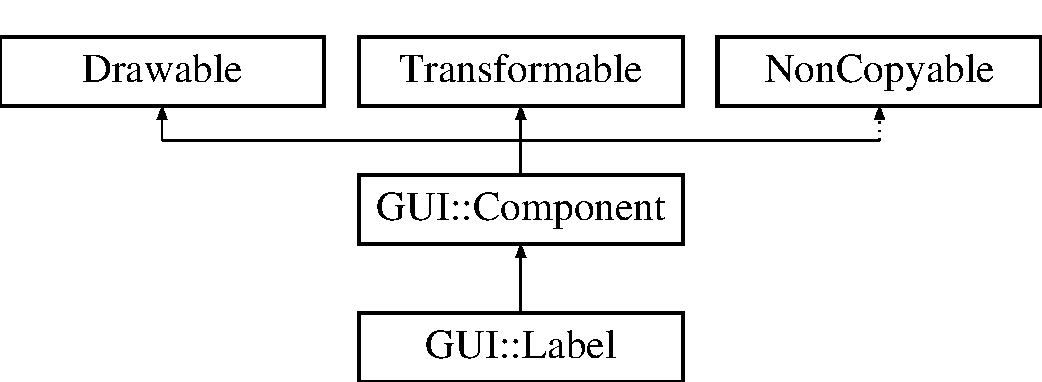
\includegraphics[height=3.000000cm]{classGUI_1_1Label}
\end{center}
\end{figure}
\subsection*{Métodos públicos}
\begin{DoxyCompactItemize}
\item 
\hyperlink{classGUI_1_1Label_afe779498111491b90a7f3a19eca9811c}{Label} (const wchar\+\_\+t $\ast$text, const \hyperlink{classResourceHolder}{Resource\+Holder}$<$ I\+D\+Fonts, sf\+::\+Font $>$ \&fonts)
\item 
virtual \hyperlink{classGUI_1_1Label_a343799d4193eb813ef561d3a479c1edd}{$\sim$\+Label} ()
\item 
virtual bool \hyperlink{classGUI_1_1Label_a4bf3538b1d2ffa440c184ad59d9b9d76}{is\+Selectable} () const 
\item 
void \hyperlink{classGUI_1_1Label_a5d274e6f5ab69563be24c71207c64ab9}{set\+Text} (const wchar\+\_\+t $\ast$text)
\item 
void \hyperlink{classGUI_1_1Label_ab86467acdbe18a9fda4712a177e16dae}{set\+Text} (const std\+::string \&text)
\item 
virtual void \hyperlink{classGUI_1_1Label_ade8d6fc5a2f56198764ee0ee0f216068}{handle\+Event} (const sf\+::\+Event \&event)
\end{DoxyCompactItemize}


\subsection{Descripción detallada}
Etiqueta G\+U\+I 

\subsection{Documentación del constructor y destructor}
\hypertarget{classGUI_1_1Label_afe779498111491b90a7f3a19eca9811c}{}\index{G\+U\+I\+::\+Label@{G\+U\+I\+::\+Label}!Label@{Label}}
\index{Label@{Label}!G\+U\+I\+::\+Label@{G\+U\+I\+::\+Label}}
\subsubsection[{Label}]{\setlength{\rightskip}{0pt plus 5cm}G\+U\+I\+::\+Label\+::\+Label (
\begin{DoxyParamCaption}
\item[{const wchar\+\_\+t $\ast$}]{text, }
\item[{const {\bf Resource\+Holder}$<$ I\+D\+Fonts, sf\+::\+Font $>$ \&}]{fonts}
\end{DoxyParamCaption}
)}\label{classGUI_1_1Label_afe779498111491b90a7f3a19eca9811c}
Constructor 
\begin{DoxyParams}{Parámetros}
{\em text} & texto de la etiqueta \\
\hline
{\em fonts} & fuentes que puede usar \\
\hline
\end{DoxyParams}
\hypertarget{classGUI_1_1Label_a343799d4193eb813ef561d3a479c1edd}{}\index{G\+U\+I\+::\+Label@{G\+U\+I\+::\+Label}!````~Label@{$\sim$\+Label}}
\index{````~Label@{$\sim$\+Label}!G\+U\+I\+::\+Label@{G\+U\+I\+::\+Label}}
\subsubsection[{$\sim$\+Label}]{\setlength{\rightskip}{0pt plus 5cm}G\+U\+I\+::\+Label\+::$\sim$\+Label (
\begin{DoxyParamCaption}
{}
\end{DoxyParamCaption}
)\hspace{0.3cm}{\ttfamily [virtual]}}\label{classGUI_1_1Label_a343799d4193eb813ef561d3a479c1edd}
Destructor 

\subsection{Documentación de las funciones miembro}
\hypertarget{classGUI_1_1Label_ade8d6fc5a2f56198764ee0ee0f216068}{}\index{G\+U\+I\+::\+Label@{G\+U\+I\+::\+Label}!handle\+Event@{handle\+Event}}
\index{handle\+Event@{handle\+Event}!G\+U\+I\+::\+Label@{G\+U\+I\+::\+Label}}
\subsubsection[{handle\+Event}]{\setlength{\rightskip}{0pt plus 5cm}void G\+U\+I\+::\+Label\+::handle\+Event (
\begin{DoxyParamCaption}
\item[{const sf\+::\+Event \&}]{event}
\end{DoxyParamCaption}
)\hspace{0.3cm}{\ttfamily [virtual]}}\label{classGUI_1_1Label_ade8d6fc5a2f56198764ee0ee0f216068}
Maneja los eventos capturados 
\begin{DoxyParams}{Parámetros}
{\em event} & evento capturado \\
\hline
\end{DoxyParams}


Implementa \hyperlink{classGUI_1_1Component_aacf5e981e7b5726f5c7e9436455660ba}{G\+U\+I\+::\+Component}.

\hypertarget{classGUI_1_1Label_a4bf3538b1d2ffa440c184ad59d9b9d76}{}\index{G\+U\+I\+::\+Label@{G\+U\+I\+::\+Label}!is\+Selectable@{is\+Selectable}}
\index{is\+Selectable@{is\+Selectable}!G\+U\+I\+::\+Label@{G\+U\+I\+::\+Label}}
\subsubsection[{is\+Selectable}]{\setlength{\rightskip}{0pt plus 5cm}bool G\+U\+I\+::\+Label\+::is\+Selectable (
\begin{DoxyParamCaption}
{}
\end{DoxyParamCaption}
) const\hspace{0.3cm}{\ttfamily [virtual]}}\label{classGUI_1_1Label_a4bf3538b1d2ffa440c184ad59d9b9d76}
Devuelve si el componente es seleccionable \begin{DoxyReturn}{Devuelve}
true si es seleccionable 
\end{DoxyReturn}


Implementa \hyperlink{classGUI_1_1Component_a44d14506c9a1dbc839e05a6bf99c341b}{G\+U\+I\+::\+Component}.

\hypertarget{classGUI_1_1Label_a5d274e6f5ab69563be24c71207c64ab9}{}\index{G\+U\+I\+::\+Label@{G\+U\+I\+::\+Label}!set\+Text@{set\+Text}}
\index{set\+Text@{set\+Text}!G\+U\+I\+::\+Label@{G\+U\+I\+::\+Label}}
\subsubsection[{set\+Text}]{\setlength{\rightskip}{0pt plus 5cm}void G\+U\+I\+::\+Label\+::set\+Text (
\begin{DoxyParamCaption}
\item[{const wchar\+\_\+t $\ast$}]{text}
\end{DoxyParamCaption}
)}\label{classGUI_1_1Label_a5d274e6f5ab69563be24c71207c64ab9}
Setea el texto de la etiqueta 
\begin{DoxyParams}{Parámetros}
{\em text} & nuevo texto \\
\hline
\end{DoxyParams}
\hypertarget{classGUI_1_1Label_ab86467acdbe18a9fda4712a177e16dae}{}\index{G\+U\+I\+::\+Label@{G\+U\+I\+::\+Label}!set\+Text@{set\+Text}}
\index{set\+Text@{set\+Text}!G\+U\+I\+::\+Label@{G\+U\+I\+::\+Label}}
\subsubsection[{set\+Text}]{\setlength{\rightskip}{0pt plus 5cm}void G\+U\+I\+::\+Label\+::set\+Text (
\begin{DoxyParamCaption}
\item[{const std\+::string \&}]{text}
\end{DoxyParamCaption}
)}\label{classGUI_1_1Label_ab86467acdbe18a9fda4712a177e16dae}
Setea el texto de la etiqueta 
\begin{DoxyParams}{Parámetros}
{\em text} & nuevo texto \\
\hline
\end{DoxyParams}


La documentación para esta clase fue generada a partir de los siguientes ficheros\+:\begin{DoxyCompactItemize}
\item 
Label.\+h\item 
Label.\+cpp\end{DoxyCompactItemize}

\hypertarget{classLevel}{}\section{Referencia de la Clase Level}
\label{classLevel}\index{Level@{Level}}


{\ttfamily \#include $<$Level.\+h$>$}

Diagrama de herencias de Level\begin{figure}[H]
\begin{center}
\leavevmode
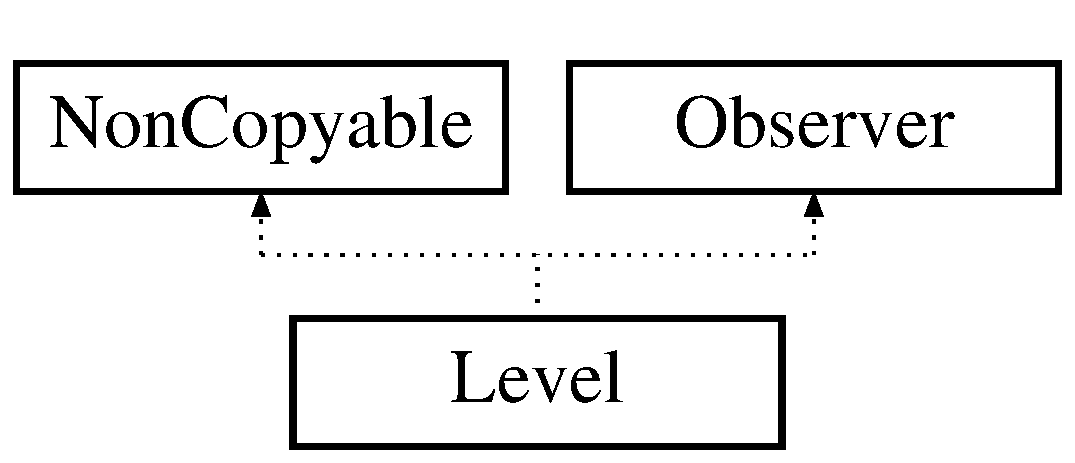
\includegraphics[height=2.000000cm]{classLevel}
\end{center}
\end{figure}
\subsection*{Métodos públicos}
\begin{DoxyCompactItemize}
\item 
\hyperlink{classLevel_ab9c7695bbbc6015fe59e4f8887764d2b}{Level} (\hyperlink{classSystemManager}{System\+Manager} \&system\+Manager)
\item 
void \hyperlink{classLevel_a67f86520cebd83af4312dc7ed26fb694}{update} (sf\+::\+Time dt)
\item 
void \hyperlink{classLevel_a16b763dfb766969c8fefec9dd11207e9}{set\+Character} (\hyperlink{classIdEntity}{Id\+Entity} character\+Created)
\item 
void \hyperlink{classLevel_a9b7478818e1aa80d3d4d059fa5faf9bf}{draw} ()
\item 
\hyperlink{classCommandQueue}{Command\+Queue} \& \hyperlink{classLevel_a9ef5d17350297a086d87b0936fec5ecb}{get\+Command\+Queue} ()
\item 
bool \hyperlink{classLevel_a135b421112c9b9a14229a59b62a82041}{handle\+Event} (const sf\+::\+Event \&event)
\item 
void \hyperlink{classLevel_a961437d70dad81b0fddb3fb728ea67af}{set\+Player} (\hyperlink{classPlayer}{Player} $\ast$player)
\item 
bool \hyperlink{classLevel_a24b4e540cca52b4d73790ce7850e62db}{is\+End} ()
\item 
Mission\+Status \hyperlink{classLevel_a6098504924fa73e05dd7a4a945b61766}{get\+Mission\+Status} ()
\item 
bool \hyperlink{classLevel_a153be085b66dc212ab9ac507c0057240}{change\+Level} ()
\item 
std\+::string $\ast$ \hyperlink{classLevel_a3d7b2e75b73bf8b459bf9a547cd923b7}{get\+Next\+Level} ()
\item 
virtual void \hyperlink{classLevel_a62e412eaad753d2baa2f94239cb80e41}{update} ()
\end{DoxyCompactItemize}


\subsection{Descripción detallada}
Clase que representa un nivel 

\subsection{Documentación del constructor y destructor}
\hypertarget{classLevel_ab9c7695bbbc6015fe59e4f8887764d2b}{}\index{Level@{Level}!Level@{Level}}
\index{Level@{Level}!Level@{Level}}
\subsubsection[{Level}]{\setlength{\rightskip}{0pt plus 5cm}Level\+::\+Level (
\begin{DoxyParamCaption}
\item[{{\bf System\+Manager} \&}]{system\+Manager}
\end{DoxyParamCaption}
)\hspace{0.3cm}{\ttfamily [explicit]}}\label{classLevel_ab9c7695bbbc6015fe59e4f8887764d2b}
Constructor explícito 
\begin{DoxyParams}{Parámetros}
{\em system\+Manager} & gestor de sistemas \\
\hline
\end{DoxyParams}


\subsection{Documentación de las funciones miembro}
\hypertarget{classLevel_a153be085b66dc212ab9ac507c0057240}{}\index{Level@{Level}!change\+Level@{change\+Level}}
\index{change\+Level@{change\+Level}!Level@{Level}}
\subsubsection[{change\+Level}]{\setlength{\rightskip}{0pt plus 5cm}bool Level\+::change\+Level (
\begin{DoxyParamCaption}
{}
\end{DoxyParamCaption}
)}\label{classLevel_a153be085b66dc212ab9ac507c0057240}
Devuelve si se ha de cambiar el nivel o no \begin{DoxyReturn}{Devuelve}
true si se ha de cambiar de nivel 
\end{DoxyReturn}
\hypertarget{classLevel_a9b7478818e1aa80d3d4d059fa5faf9bf}{}\index{Level@{Level}!draw@{draw}}
\index{draw@{draw}!Level@{Level}}
\subsubsection[{draw}]{\setlength{\rightskip}{0pt plus 5cm}void Level\+::draw (
\begin{DoxyParamCaption}
{}
\end{DoxyParamCaption}
)}\label{classLevel_a9b7478818e1aa80d3d4d059fa5faf9bf}
Dibuja el nivel \hypertarget{classLevel_a9ef5d17350297a086d87b0936fec5ecb}{}\index{Level@{Level}!get\+Command\+Queue@{get\+Command\+Queue}}
\index{get\+Command\+Queue@{get\+Command\+Queue}!Level@{Level}}
\subsubsection[{get\+Command\+Queue}]{\setlength{\rightskip}{0pt plus 5cm}{\bf Command\+Queue}\& Level\+::get\+Command\+Queue (
\begin{DoxyParamCaption}
{}
\end{DoxyParamCaption}
)\hspace{0.3cm}{\ttfamily [inline]}}\label{classLevel_a9ef5d17350297a086d87b0936fec5ecb}
Devuelve la cola de comandos \begin{DoxyReturn}{Devuelve}
cola de comandos 
\end{DoxyReturn}
\hypertarget{classLevel_a6098504924fa73e05dd7a4a945b61766}{}\index{Level@{Level}!get\+Mission\+Status@{get\+Mission\+Status}}
\index{get\+Mission\+Status@{get\+Mission\+Status}!Level@{Level}}
\subsubsection[{get\+Mission\+Status}]{\setlength{\rightskip}{0pt plus 5cm}Mission\+Status Level\+::get\+Mission\+Status (
\begin{DoxyParamCaption}
{}
\end{DoxyParamCaption}
)\hspace{0.3cm}{\ttfamily [inline]}}\label{classLevel_a6098504924fa73e05dd7a4a945b61766}
Pilla el estado de la misión \begin{DoxyReturn}{Devuelve}

\end{DoxyReturn}
\hypertarget{classLevel_a3d7b2e75b73bf8b459bf9a547cd923b7}{}\index{Level@{Level}!get\+Next\+Level@{get\+Next\+Level}}
\index{get\+Next\+Level@{get\+Next\+Level}!Level@{Level}}
\subsubsection[{get\+Next\+Level}]{\setlength{\rightskip}{0pt plus 5cm}std\+::string $\ast$ Level\+::get\+Next\+Level (
\begin{DoxyParamCaption}
{}
\end{DoxyParamCaption}
)}\label{classLevel_a3d7b2e75b73bf8b459bf9a547cd923b7}
Devuelve el siguiente nivel que se carga \begin{DoxyReturn}{Devuelve}

\end{DoxyReturn}
\hypertarget{classLevel_a135b421112c9b9a14229a59b62a82041}{}\index{Level@{Level}!handle\+Event@{handle\+Event}}
\index{handle\+Event@{handle\+Event}!Level@{Level}}
\subsubsection[{handle\+Event}]{\setlength{\rightskip}{0pt plus 5cm}bool Level\+::handle\+Event (
\begin{DoxyParamCaption}
\item[{const sf\+::\+Event \&}]{event}
\end{DoxyParamCaption}
)}\label{classLevel_a135b421112c9b9a14229a59b62a82041}
Procesa la entrada \hypertarget{classLevel_a24b4e540cca52b4d73790ce7850e62db}{}\index{Level@{Level}!is\+End@{is\+End}}
\index{is\+End@{is\+End}!Level@{Level}}
\subsubsection[{is\+End}]{\setlength{\rightskip}{0pt plus 5cm}bool Level\+::is\+End (
\begin{DoxyParamCaption}
{}
\end{DoxyParamCaption}
)}\label{classLevel_a24b4e540cca52b4d73790ce7850e62db}
Determina si el nivel ha terminado \begin{DoxyReturn}{Devuelve}
true si el nivel ha terminado 
\end{DoxyReturn}
\hypertarget{classLevel_a16b763dfb766969c8fefec9dd11207e9}{}\index{Level@{Level}!set\+Character@{set\+Character}}
\index{set\+Character@{set\+Character}!Level@{Level}}
\subsubsection[{set\+Character}]{\setlength{\rightskip}{0pt plus 5cm}void Level\+::set\+Character (
\begin{DoxyParamCaption}
\item[{{\bf Id\+Entity}}]{character\+Created}
\end{DoxyParamCaption}
)}\label{classLevel_a16b763dfb766969c8fefec9dd11207e9}
Setea el personaje principal 
\begin{DoxyParams}{Parámetros}
{\em character\+Created} & entidad del personaje \\
\hline
\end{DoxyParams}
\hypertarget{classLevel_a961437d70dad81b0fddb3fb728ea67af}{}\index{Level@{Level}!set\+Player@{set\+Player}}
\index{set\+Player@{set\+Player}!Level@{Level}}
\subsubsection[{set\+Player}]{\setlength{\rightskip}{0pt plus 5cm}void Level\+::set\+Player (
\begin{DoxyParamCaption}
\item[{{\bf Player} $\ast$}]{player}
\end{DoxyParamCaption}
)\hspace{0.3cm}{\ttfamily [inline]}}\label{classLevel_a961437d70dad81b0fddb3fb728ea67af}
Setea el jugador (captura de eventos) 
\begin{DoxyParams}{Parámetros}
{\em player} & jugador \\
\hline
\end{DoxyParams}
\hypertarget{classLevel_a67f86520cebd83af4312dc7ed26fb694}{}\index{Level@{Level}!update@{update}}
\index{update@{update}!Level@{Level}}
\subsubsection[{update}]{\setlength{\rightskip}{0pt plus 5cm}void Level\+::update (
\begin{DoxyParamCaption}
\item[{sf\+::\+Time}]{dt}
\end{DoxyParamCaption}
)}\label{classLevel_a67f86520cebd83af4312dc7ed26fb694}
Actualiza el nivel 
\begin{DoxyParams}{Parámetros}
{\em dt} & tiempo entre frame y frame \\
\hline
\end{DoxyParams}
\hypertarget{classLevel_a62e412eaad753d2baa2f94239cb80e41}{}\index{Level@{Level}!update@{update}}
\index{update@{update}!Level@{Level}}
\subsubsection[{update}]{\setlength{\rightskip}{0pt plus 5cm}void Level\+::update (
\begin{DoxyParamCaption}
{}
\end{DoxyParamCaption}
)\hspace{0.3cm}{\ttfamily [virtual]}}\label{classLevel_a62e412eaad753d2baa2f94239cb80e41}
Actualiza los subestados del juego cuando hay cambios 

Implementa \hyperlink{classObserver_ac75e4b339faeb3ea6fe0a01bf0b4a215}{Observer}.



La documentación para esta clase fue generada a partir de los siguientes ficheros\+:\begin{DoxyCompactItemize}
\item 
Level.\+h\item 
Level.\+cpp\end{DoxyCompactItemize}

\hypertarget{classLife}{}\section{Referencia de la Clase Life}
\label{classLife}\index{Life@{Life}}


{\ttfamily \#include $<$Life.\+h$>$}

\subsection*{Métodos públicos}
\begin{DoxyCompactItemize}
\item 
\hyperlink{classLife_a6de2a371f6f778f8b4938d219390b746}{Life} ()
\item 
\hyperlink{classLife_a2964d51ba57add1054e4dca7b9267511}{Life} (int max\+Life)
\item 
\hyperlink{classLife_a5654f86257b68469dd966eed44a5d1d6}{Life} (const \hyperlink{classLife}{Life} \&orig)
\item 
virtual \hyperlink{classLife_ac5a521e06906fb4f834001b2b4f7adc7}{$\sim$\+Life} ()
\item 
int \hyperlink{classLife_adc50ff45896057a22eff164c26ff2c97}{get\+Actual\+Life} () const 
\item 
void \hyperlink{classLife_afc63b290a513272974e117191326d175}{set\+Actual\+Life} (int actual\+Life)
\item 
int \hyperlink{classLife_ad14340558348956867f68369a2b0f642}{get\+Max\+Life} () const 
\item 
void \hyperlink{classLife_ad02aacd2902ea4e626aa6bf45dc53e49}{set\+Max\+Life} (int max\+Life)
\item 
void \hyperlink{classLife_aa9fb062c056f19b5cc0bf60360dfff73}{damage} (int damage)
\item 
bool \hyperlink{classLife_ad596f5eaf723c8188a8043beb0437ef2}{is\+Alive} ()
\end{DoxyCompactItemize}


\subsection{Descripción detallada}
Clase representando una vida 

\subsection{Documentación del constructor y destructor}
\hypertarget{classLife_a6de2a371f6f778f8b4938d219390b746}{}\index{Life@{Life}!Life@{Life}}
\index{Life@{Life}!Life@{Life}}
\subsubsection[{Life}]{\setlength{\rightskip}{0pt plus 5cm}Life\+::\+Life (
\begin{DoxyParamCaption}
{}
\end{DoxyParamCaption}
)}\label{classLife_a6de2a371f6f778f8b4938d219390b746}
Constructor por defecto dejando una vida de 100 unidades \hypertarget{classLife_a2964d51ba57add1054e4dca7b9267511}{}\index{Life@{Life}!Life@{Life}}
\index{Life@{Life}!Life@{Life}}
\subsubsection[{Life}]{\setlength{\rightskip}{0pt plus 5cm}Life\+::\+Life (
\begin{DoxyParamCaption}
\item[{int}]{max\+Life}
\end{DoxyParamCaption}
)}\label{classLife_a2964d51ba57add1054e4dca7b9267511}
C\+Onstructor especificando el máximo de vida 
\begin{DoxyParams}{Parámetros}
{\em max\+Life} & máximo de vida \\
\hline
\end{DoxyParams}
\hypertarget{classLife_a5654f86257b68469dd966eed44a5d1d6}{}\index{Life@{Life}!Life@{Life}}
\index{Life@{Life}!Life@{Life}}
\subsubsection[{Life}]{\setlength{\rightskip}{0pt plus 5cm}Life\+::\+Life (
\begin{DoxyParamCaption}
\item[{const {\bf Life} \&}]{orig}
\end{DoxyParamCaption}
)}\label{classLife_a5654f86257b68469dd966eed44a5d1d6}
Constructor copia 
\begin{DoxyParams}{Parámetros}
{\em orig} & vida a copiar \\
\hline
\end{DoxyParams}
\hypertarget{classLife_ac5a521e06906fb4f834001b2b4f7adc7}{}\index{Life@{Life}!````~Life@{$\sim$\+Life}}
\index{````~Life@{$\sim$\+Life}!Life@{Life}}
\subsubsection[{$\sim$\+Life}]{\setlength{\rightskip}{0pt plus 5cm}Life\+::$\sim$\+Life (
\begin{DoxyParamCaption}
{}
\end{DoxyParamCaption}
)\hspace{0.3cm}{\ttfamily [virtual]}}\label{classLife_ac5a521e06906fb4f834001b2b4f7adc7}
Destructor 

\subsection{Documentación de las funciones miembro}
\hypertarget{classLife_aa9fb062c056f19b5cc0bf60360dfff73}{}\index{Life@{Life}!damage@{damage}}
\index{damage@{damage}!Life@{Life}}
\subsubsection[{damage}]{\setlength{\rightskip}{0pt plus 5cm}void Life\+::damage (
\begin{DoxyParamCaption}
\item[{int}]{damage}
\end{DoxyParamCaption}
)}\label{classLife_aa9fb062c056f19b5cc0bf60360dfff73}
Establece un daño, decrementa la vida en las unidades especificadas 
\begin{DoxyParams}{Parámetros}
{\em damage} & unidades a decrementar la vida \\
\hline
\end{DoxyParams}
\hypertarget{classLife_adc50ff45896057a22eff164c26ff2c97}{}\index{Life@{Life}!get\+Actual\+Life@{get\+Actual\+Life}}
\index{get\+Actual\+Life@{get\+Actual\+Life}!Life@{Life}}
\subsubsection[{get\+Actual\+Life}]{\setlength{\rightskip}{0pt plus 5cm}int Life\+::get\+Actual\+Life (
\begin{DoxyParamCaption}
{}
\end{DoxyParamCaption}
) const\hspace{0.3cm}{\ttfamily [inline]}}\label{classLife_adc50ff45896057a22eff164c26ff2c97}
Devuelve la vida actual \begin{DoxyReturn}{Devuelve}
devuelve la vida actual que le queda 
\end{DoxyReturn}
\hypertarget{classLife_ad14340558348956867f68369a2b0f642}{}\index{Life@{Life}!get\+Max\+Life@{get\+Max\+Life}}
\index{get\+Max\+Life@{get\+Max\+Life}!Life@{Life}}
\subsubsection[{get\+Max\+Life}]{\setlength{\rightskip}{0pt plus 5cm}int Life\+::get\+Max\+Life (
\begin{DoxyParamCaption}
{}
\end{DoxyParamCaption}
) const\hspace{0.3cm}{\ttfamily [inline]}}\label{classLife_ad14340558348956867f68369a2b0f642}
Devuelve la vida máxima \begin{DoxyReturn}{Devuelve}
vida máxima 
\end{DoxyReturn}
\hypertarget{classLife_ad596f5eaf723c8188a8043beb0437ef2}{}\index{Life@{Life}!is\+Alive@{is\+Alive}}
\index{is\+Alive@{is\+Alive}!Life@{Life}}
\subsubsection[{is\+Alive}]{\setlength{\rightskip}{0pt plus 5cm}bool Life\+::is\+Alive (
\begin{DoxyParamCaption}
{}
\end{DoxyParamCaption}
)}\label{classLife_ad596f5eaf723c8188a8043beb0437ef2}
Determina si está vivo, es decir, si la vida es mayor de 0 \begin{DoxyReturn}{Devuelve}
true si está vivo 
\end{DoxyReturn}
\hypertarget{classLife_afc63b290a513272974e117191326d175}{}\index{Life@{Life}!set\+Actual\+Life@{set\+Actual\+Life}}
\index{set\+Actual\+Life@{set\+Actual\+Life}!Life@{Life}}
\subsubsection[{set\+Actual\+Life}]{\setlength{\rightskip}{0pt plus 5cm}void Life\+::set\+Actual\+Life (
\begin{DoxyParamCaption}
\item[{int}]{actual\+Life}
\end{DoxyParamCaption}
)\hspace{0.3cm}{\ttfamily [inline]}}\label{classLife_afc63b290a513272974e117191326d175}
Setea la vida 
\begin{DoxyParams}{Parámetros}
{\em actual\+Life} & vida actual a setear \\
\hline
\end{DoxyParams}
\hypertarget{classLife_ad02aacd2902ea4e626aa6bf45dc53e49}{}\index{Life@{Life}!set\+Max\+Life@{set\+Max\+Life}}
\index{set\+Max\+Life@{set\+Max\+Life}!Life@{Life}}
\subsubsection[{set\+Max\+Life}]{\setlength{\rightskip}{0pt plus 5cm}void Life\+::set\+Max\+Life (
\begin{DoxyParamCaption}
\item[{int}]{max\+Life}
\end{DoxyParamCaption}
)\hspace{0.3cm}{\ttfamily [inline]}}\label{classLife_ad02aacd2902ea4e626aa6bf45dc53e49}
Setea la vida máxima 
\begin{DoxyParams}{Parámetros}
{\em max\+Life} & vida máxima a setear \\
\hline
\end{DoxyParams}


La documentación para esta clase fue generada a partir de los siguientes ficheros\+:\begin{DoxyCompactItemize}
\item 
Life.\+h\item 
Life.\+cpp\end{DoxyCompactItemize}

\hypertarget{classLifeNode}{}\section{Referencia de la Clase Life\+Node}
\label{classLifeNode}\index{Life\+Node@{Life\+Node}}


{\ttfamily \#include $<$Life\+Node.\+h$>$}

Diagrama de herencias de Life\+Node\begin{figure}[H]
\begin{center}
\leavevmode
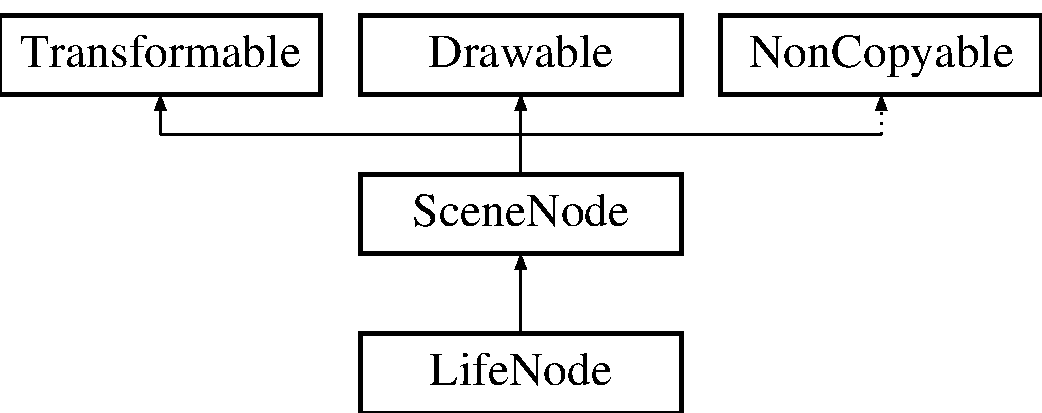
\includegraphics[height=3.000000cm]{classLifeNode}
\end{center}
\end{figure}
\subsection*{Métodos públicos}
\begin{DoxyCompactItemize}
\item 
\hyperlink{classLifeNode_a2668b18add55f48c23dae62b2129c68f}{Life\+Node} (\hyperlink{classResourceHolder}{Resource\+Holder}$<$ std\+::string, sf\+::\+Texture $>$ \&texture, \hyperlink{classLife}{Life} \&life, sf\+::\+Vector2f size)
\end{DoxyCompactItemize}
\subsection*{Otros miembros heredados}


\subsection{Descripción detallada}
Nodo que representa la vida de una entidad 

\subsection{Documentación del constructor y destructor}
\hypertarget{classLifeNode_a2668b18add55f48c23dae62b2129c68f}{}\index{Life\+Node@{Life\+Node}!Life\+Node@{Life\+Node}}
\index{Life\+Node@{Life\+Node}!Life\+Node@{Life\+Node}}
\subsubsection[{Life\+Node}]{\setlength{\rightskip}{0pt plus 5cm}Life\+Node\+::\+Life\+Node (
\begin{DoxyParamCaption}
\item[{{\bf Resource\+Holder}$<$ std\+::string, sf\+::\+Texture $>$ \&}]{texture, }
\item[{{\bf Life} \&}]{life, }
\item[{sf\+::\+Vector2f}]{size}
\end{DoxyParamCaption}
)}\label{classLifeNode_a2668b18add55f48c23dae62b2129c68f}

\begin{DoxyParams}{Parámetros}
{\em texture} & imagenes \\
\hline
{\em life} & la vida de la entidad \\
\hline
{\em size} & el tamaño que se desea para el dibujado \\
\hline
\end{DoxyParams}


La documentación para esta clase fue generada a partir de los siguientes ficheros\+:\begin{DoxyCompactItemize}
\item 
Life\+Node.\+h\item 
Life\+Node.\+cpp\end{DoxyCompactItemize}

\hypertarget{classLoadingLevel}{}\section{Referencia de la Clase Loading\+Level}
\label{classLoadingLevel}\index{Loading\+Level@{Loading\+Level}}


{\ttfamily \#include $<$Loading\+Level.\+h$>$}

Diagrama de herencias de Loading\+Level\begin{figure}[H]
\begin{center}
\leavevmode
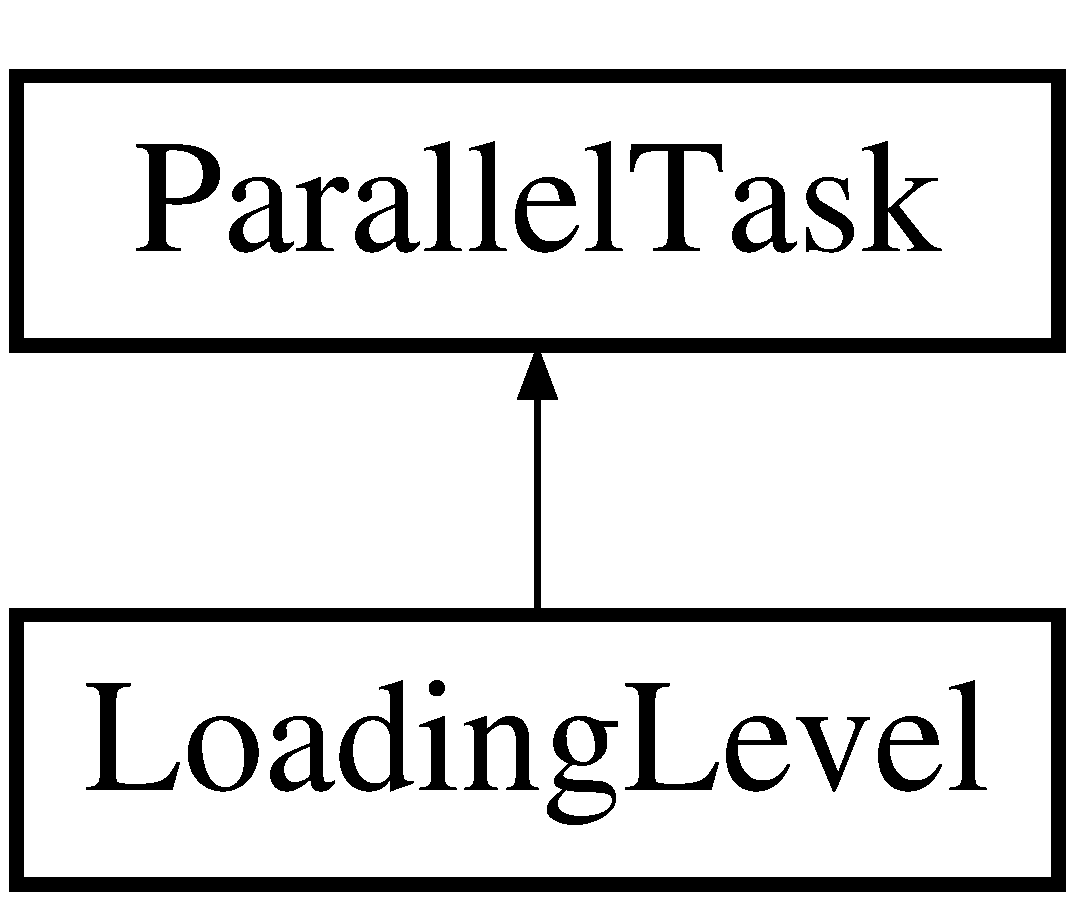
\includegraphics[height=2.000000cm]{classLoadingLevel}
\end{center}
\end{figure}
\subsection*{Métodos públicos}
\begin{DoxyCompactItemize}
\item 
\hyperlink{classLoadingLevel_a213ac5771607d12a05d5f43726d46d5e}{Loading\+Level} (std\+::string $\ast$level, \hyperlink{classContext}{Context} $\ast$context)
\item 
virtual void \hyperlink{classLoadingLevel_a14f8ce9f74732609e4da6c8cce387001}{run\+Task} ()
\end{DoxyCompactItemize}
\subsection*{Otros miembros heredados}


\subsection{Descripción detallada}
Tarea paralela para cargar un nivel 

\subsection{Documentación del constructor y destructor}
\hypertarget{classLoadingLevel_a213ac5771607d12a05d5f43726d46d5e}{}\index{Loading\+Level@{Loading\+Level}!Loading\+Level@{Loading\+Level}}
\index{Loading\+Level@{Loading\+Level}!Loading\+Level@{Loading\+Level}}
\subsubsection[{Loading\+Level}]{\setlength{\rightskip}{0pt plus 5cm}Loading\+Level\+::\+Loading\+Level (
\begin{DoxyParamCaption}
\item[{std\+::string $\ast$}]{level, }
\item[{{\bf Context} $\ast$}]{context}
\end{DoxyParamCaption}
)}\label{classLoadingLevel_a213ac5771607d12a05d5f43726d46d5e}
Constructor 
\begin{DoxyParams}{Parámetros}
{\em level} & nombre/ruta del nivel a cargar \\
\hline
{\em context} & contexto de la aplicación \\
\hline
\end{DoxyParams}


\subsection{Documentación de las funciones miembro}
\hypertarget{classLoadingLevel_a14f8ce9f74732609e4da6c8cce387001}{}\index{Loading\+Level@{Loading\+Level}!run\+Task@{run\+Task}}
\index{run\+Task@{run\+Task}!Loading\+Level@{Loading\+Level}}
\subsubsection[{run\+Task}]{\setlength{\rightskip}{0pt plus 5cm}void Loading\+Level\+::run\+Task (
\begin{DoxyParamCaption}
{}
\end{DoxyParamCaption}
)\hspace{0.3cm}{\ttfamily [virtual]}}\label{classLoadingLevel_a14f8ce9f74732609e4da6c8cce387001}
Método a sobreescribir. En él se codifica la tarea a realizar 

Implementa \hyperlink{classParallelTask_a494412a04608d42f3ba91b1b242fd149}{Parallel\+Task}.



La documentación para esta clase fue generada a partir de los siguientes ficheros\+:\begin{DoxyCompactItemize}
\item 
Loading\+Level.\+h\item 
Loading\+Level.\+cpp\end{DoxyCompactItemize}

\hypertarget{classLoadingState}{}\section{Referencia de la Clase Loading\+State}
\label{classLoadingState}\index{Loading\+State@{Loading\+State}}


{\ttfamily \#include $<$Loading\+State.\+h$>$}

Diagrama de herencias de Loading\+State\begin{figure}[H]
\begin{center}
\leavevmode
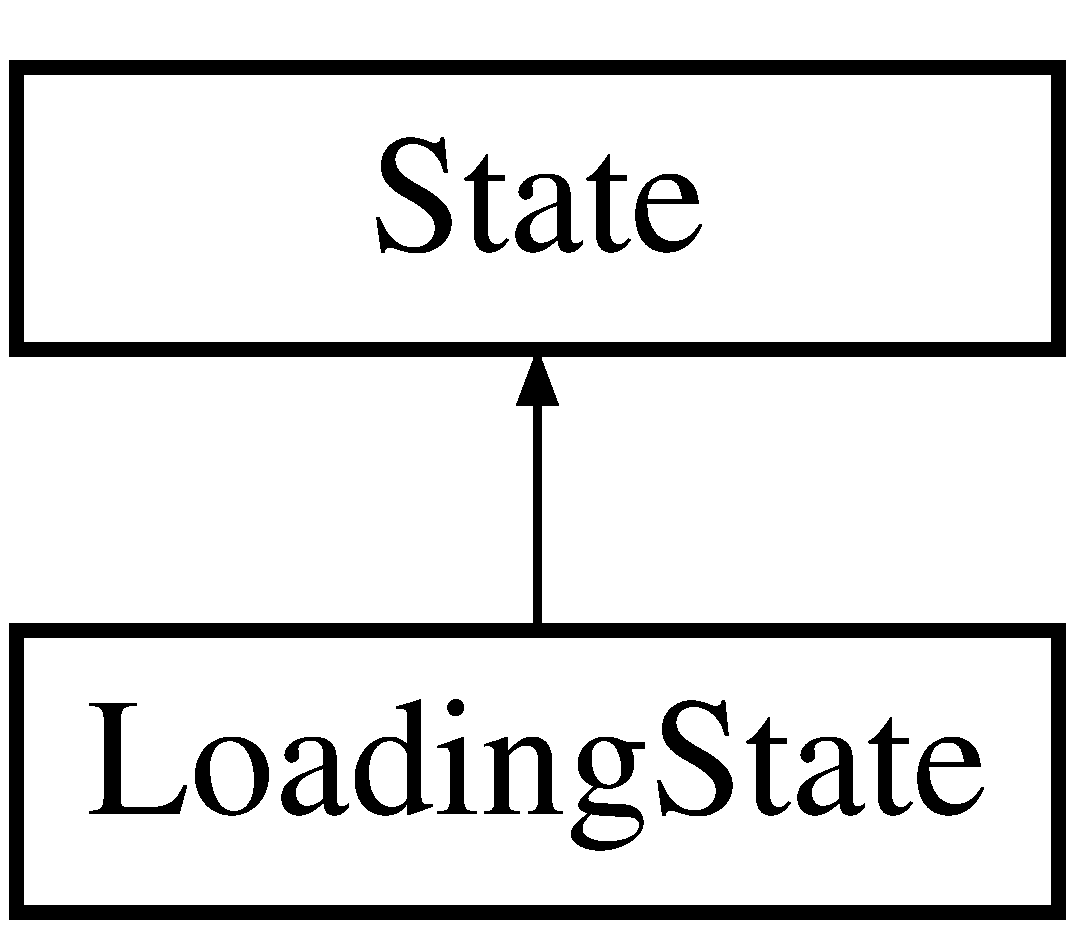
\includegraphics[height=2.000000cm]{classLoadingState}
\end{center}
\end{figure}
\subsection*{Métodos públicos}
\begin{DoxyCompactItemize}
\item 
\hypertarget{classLoadingState_a44c4ab240d82642ff91498380c9d34d0}{}{\bfseries Loading\+State} (\hyperlink{classStateStack}{State\+Stack} \&\hyperlink{classState_a86c8d3a5a1ee89896828be85a785fb04}{stack}, \hyperlink{classContext}{Context} $\ast$\hyperlink{classState_adc93e8ad3199b5891618ca88eed0436a}{context})\label{classLoadingState_a44c4ab240d82642ff91498380c9d34d0}

\item 
virtual void \hyperlink{classLoadingState_adfe2c002c52cc2c49967ba3ace4aa73b}{draw} ()
\item 
virtual bool \hyperlink{classLoadingState_a8f1729b9b5ca91c0ec3918b86bfe8feb}{update} (sf\+::\+Time delta)
\item 
virtual bool \hyperlink{classLoadingState_a37da243eeeca36460bac2f32cef3e368}{handle\+Event} (const sf\+::\+Event \&event)
\item 
void \hyperlink{classLoadingState_a28bee93e7f9818084af8be6b31ee0ba4}{set\+Completion} (float percent)
\end{DoxyCompactItemize}
\subsection*{Otros miembros heredados}


\subsection{Descripción detallada}
Estado de carga 

\subsection{Documentación de las funciones miembro}
\hypertarget{classLoadingState_adfe2c002c52cc2c49967ba3ace4aa73b}{}\index{Loading\+State@{Loading\+State}!draw@{draw}}
\index{draw@{draw}!Loading\+State@{Loading\+State}}
\subsubsection[{draw}]{\setlength{\rightskip}{0pt plus 5cm}void Loading\+State\+::draw (
\begin{DoxyParamCaption}
{}
\end{DoxyParamCaption}
)\hspace{0.3cm}{\ttfamily [virtual]}}\label{classLoadingState_adfe2c002c52cc2c49967ba3ace4aa73b}
Dibuja el estado 

Implementa \hyperlink{classState_ae261605bc40b7e3959ce5df5457e4942}{State}.

\hypertarget{classLoadingState_a37da243eeeca36460bac2f32cef3e368}{}\index{Loading\+State@{Loading\+State}!handle\+Event@{handle\+Event}}
\index{handle\+Event@{handle\+Event}!Loading\+State@{Loading\+State}}
\subsubsection[{handle\+Event}]{\setlength{\rightskip}{0pt plus 5cm}bool Loading\+State\+::handle\+Event (
\begin{DoxyParamCaption}
\item[{const sf\+::\+Event \&}]{event}
\end{DoxyParamCaption}
)\hspace{0.3cm}{\ttfamily [virtual]}}\label{classLoadingState_a37da243eeeca36460bac2f32cef3e368}
Procesa la entrada del usuario 
\begin{DoxyParams}{Parámetros}
{\em event} & evento \\
\hline
\end{DoxyParams}
\begin{DoxyReturn}{Devuelve}
true si lo ha procesado, false si no (o lo ha procesado pero que continúe) 
\end{DoxyReturn}


Implementa \hyperlink{classState_a19965f83460b248c42952aac8d001206}{State}.

\hypertarget{classLoadingState_a28bee93e7f9818084af8be6b31ee0ba4}{}\index{Loading\+State@{Loading\+State}!set\+Completion@{set\+Completion}}
\index{set\+Completion@{set\+Completion}!Loading\+State@{Loading\+State}}
\subsubsection[{set\+Completion}]{\setlength{\rightskip}{0pt plus 5cm}void Loading\+State\+::set\+Completion (
\begin{DoxyParamCaption}
\item[{float}]{percent}
\end{DoxyParamCaption}
)}\label{classLoadingState_a28bee93e7f9818084af8be6b31ee0ba4}
Establece el porcentaje de completado, modificando la barra de progeso acorde 
\begin{DoxyParams}{Parámetros}
{\em percent} & porcentaje de 0 a 100 completado \\
\hline
\end{DoxyParams}
\hypertarget{classLoadingState_a8f1729b9b5ca91c0ec3918b86bfe8feb}{}\index{Loading\+State@{Loading\+State}!update@{update}}
\index{update@{update}!Loading\+State@{Loading\+State}}
\subsubsection[{update}]{\setlength{\rightskip}{0pt plus 5cm}bool Loading\+State\+::update (
\begin{DoxyParamCaption}
\item[{sf\+::\+Time}]{delta}
\end{DoxyParamCaption}
)\hspace{0.3cm}{\ttfamily [virtual]}}\label{classLoadingState_a8f1729b9b5ca91c0ec3918b86bfe8feb}
Actualiza el estado 
\begin{DoxyParams}{Parámetros}
{\em delta} & tiempo entre frame y frame \\
\hline
\end{DoxyParams}
\begin{DoxyReturn}{Devuelve}
true si se ha actualizado 
\end{DoxyReturn}


Implementa \hyperlink{classState_aa6366828eb50639e86b94008cfad9c5d}{State}.



La documentación para esta clase fue generada a partir de los siguientes ficheros\+:\begin{DoxyCompactItemize}
\item 
Loading\+State.\+h\item 
Loading\+State.\+cpp\end{DoxyCompactItemize}

\hypertarget{classMenuState}{}\section{Referencia de la Clase Menu\+State}
\label{classMenuState}\index{Menu\+State@{Menu\+State}}


{\ttfamily \#include $<$Menu\+State.\+h$>$}

Diagrama de herencias de Menu\+State\begin{figure}[H]
\begin{center}
\leavevmode
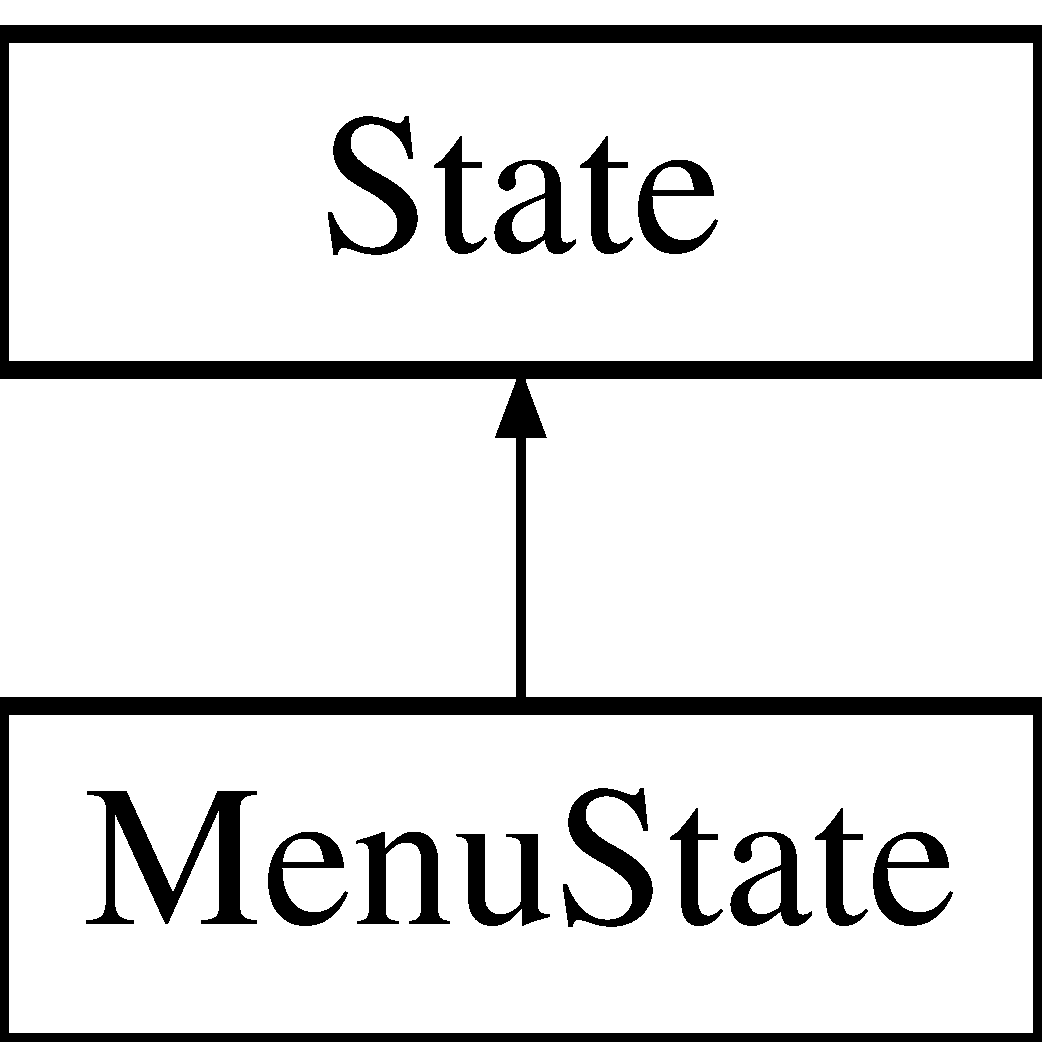
\includegraphics[height=2.000000cm]{classMenuState}
\end{center}
\end{figure}
\subsection*{Métodos públicos}
\begin{DoxyCompactItemize}
\item 
\hypertarget{classMenuState_a1ad806f354ec6b688a3c7b1bfcda9846}{}{\bfseries Menu\+State} (\hyperlink{classStateStack}{State\+Stack} \&\hyperlink{classState_a86c8d3a5a1ee89896828be85a785fb04}{stack}, \hyperlink{classContext}{Context} $\ast$\hyperlink{classState_adc93e8ad3199b5891618ca88eed0436a}{context})\label{classMenuState_a1ad806f354ec6b688a3c7b1bfcda9846}

\item 
virtual void \hyperlink{classMenuState_aa557d6c3bf06bb3107ed780913a6b47f}{draw} ()
\item 
virtual bool \hyperlink{classMenuState_a24362f4096e0f76e02a7d1b26ac657af}{update} (sf\+::\+Time delta)
\item 
virtual bool \hyperlink{classMenuState_a04a21241cebf6a8f0fe8ee9ce895ef18}{handle\+Event} (const sf\+::\+Event \&event)
\item 
virtual void \hyperlink{classMenuState_aa465ec731c1ab2b63a54ce5c59092ea3}{pulled\+Action} ()
\item 
virtual void \hyperlink{classMenuState_a74beed2b1d43948dd7ab1b8262519df6}{pushed\+Action} ()
\end{DoxyCompactItemize}
\subsection*{Otros miembros heredados}


\subsection{Descripción detallada}
Estado para el menú principal 

\subsection{Documentación de las funciones miembro}
\hypertarget{classMenuState_aa557d6c3bf06bb3107ed780913a6b47f}{}\index{Menu\+State@{Menu\+State}!draw@{draw}}
\index{draw@{draw}!Menu\+State@{Menu\+State}}
\subsubsection[{draw}]{\setlength{\rightskip}{0pt plus 5cm}void Menu\+State\+::draw (
\begin{DoxyParamCaption}
{}
\end{DoxyParamCaption}
)\hspace{0.3cm}{\ttfamily [virtual]}}\label{classMenuState_aa557d6c3bf06bb3107ed780913a6b47f}
Dibuja el estado 

Implementa \hyperlink{classState_ae261605bc40b7e3959ce5df5457e4942}{State}.

\hypertarget{classMenuState_a04a21241cebf6a8f0fe8ee9ce895ef18}{}\index{Menu\+State@{Menu\+State}!handle\+Event@{handle\+Event}}
\index{handle\+Event@{handle\+Event}!Menu\+State@{Menu\+State}}
\subsubsection[{handle\+Event}]{\setlength{\rightskip}{0pt plus 5cm}bool Menu\+State\+::handle\+Event (
\begin{DoxyParamCaption}
\item[{const sf\+::\+Event \&}]{event}
\end{DoxyParamCaption}
)\hspace{0.3cm}{\ttfamily [virtual]}}\label{classMenuState_a04a21241cebf6a8f0fe8ee9ce895ef18}
Procesa la entrada del usuario 
\begin{DoxyParams}{Parámetros}
{\em event} & evento \\
\hline
\end{DoxyParams}
\begin{DoxyReturn}{Devuelve}
true si lo ha procesado, false si no (o lo ha procesado pero que continúe) 
\end{DoxyReturn}


Implementa \hyperlink{classState_a19965f83460b248c42952aac8d001206}{State}.

\hypertarget{classMenuState_aa465ec731c1ab2b63a54ce5c59092ea3}{}\index{Menu\+State@{Menu\+State}!pulled\+Action@{pulled\+Action}}
\index{pulled\+Action@{pulled\+Action}!Menu\+State@{Menu\+State}}
\subsubsection[{pulled\+Action}]{\setlength{\rightskip}{0pt plus 5cm}void Menu\+State\+::pulled\+Action (
\begin{DoxyParamCaption}
{}
\end{DoxyParamCaption}
)\hspace{0.3cm}{\ttfamily [virtual]}}\label{classMenuState_aa465ec731c1ab2b63a54ce5c59092ea3}
Método ejecutado cuando es sacado de la pila 

Reimplementado de \hyperlink{classState_a92620c4648de675037b20ec59edb52a3}{State}.

\hypertarget{classMenuState_a74beed2b1d43948dd7ab1b8262519df6}{}\index{Menu\+State@{Menu\+State}!pushed\+Action@{pushed\+Action}}
\index{pushed\+Action@{pushed\+Action}!Menu\+State@{Menu\+State}}
\subsubsection[{pushed\+Action}]{\setlength{\rightskip}{0pt plus 5cm}void Menu\+State\+::pushed\+Action (
\begin{DoxyParamCaption}
{}
\end{DoxyParamCaption}
)\hspace{0.3cm}{\ttfamily [virtual]}}\label{classMenuState_a74beed2b1d43948dd7ab1b8262519df6}
Método ejecutado cuando es puesto en pila 

Reimplementado de \hyperlink{classState_a3cc6a1378f32f9ed6a2d1d8140296808}{State}.

\hypertarget{classMenuState_a24362f4096e0f76e02a7d1b26ac657af}{}\index{Menu\+State@{Menu\+State}!update@{update}}
\index{update@{update}!Menu\+State@{Menu\+State}}
\subsubsection[{update}]{\setlength{\rightskip}{0pt plus 5cm}bool Menu\+State\+::update (
\begin{DoxyParamCaption}
\item[{sf\+::\+Time}]{delta}
\end{DoxyParamCaption}
)\hspace{0.3cm}{\ttfamily [virtual]}}\label{classMenuState_a24362f4096e0f76e02a7d1b26ac657af}
Actualiza el estado 
\begin{DoxyParams}{Parámetros}
{\em delta} & tiempo entre frame y frame \\
\hline
\end{DoxyParams}
\begin{DoxyReturn}{Devuelve}
true si se ha actualizado 
\end{DoxyReturn}


Implementa \hyperlink{classState_aa6366828eb50639e86b94008cfad9c5d}{State}.



La documentación para esta clase fue generada a partir de los siguientes ficheros\+:\begin{DoxyCompactItemize}
\item 
Menu\+State.\+h\item 
Menu\+State.\+cpp\end{DoxyCompactItemize}

\hypertarget{classMessage}{}\section{Referencia de la Clase Message}
\label{classMessage}\index{Message@{Message}}


{\ttfamily \#include $<$Message.\+h$>$}

\subsection*{Métodos públicos}
\begin{DoxyCompactItemize}
\item 
\hyperlink{classMessage_a4fc4f717b634e66070366cb7722d7761}{Message} ()
\item 
\hyperlink{classMessage_aea145be2c9b61e83ea5fc5ecc076cf13}{Message} (Game\+States state)
\item 
Game\+States \hyperlink{classMessage_aa50d9a886ab478eff2455adc1fe55bde}{get\+State} () const 
\item 
void \hyperlink{classMessage_ac744e76db938f119be824b22d6dd8156}{set\+State} (Game\+States state)
\item 
\hyperlink{classIdEntity}{Id\+Entity} \hyperlink{classMessage_a18e8816b662ce9b4df16279743b17db0}{get\+Id\+Entity} () const 
\item 
void \hyperlink{classMessage_a77ef2e887c2bf958d970f0a240243b65}{set\+Id\+Entity} (\hyperlink{classIdEntity}{Id\+Entity} id)
\item 
void \hyperlink{classMessage_ac3df51b5a409d4962768e6d0d8595f2f}{set\+Data} (std\+::string $\ast$data)
\item 
std\+::string $\ast$ \hyperlink{classMessage_a18d2d59a27010dd396f2842dbf6ecfc2}{get\+Data} ()
\end{DoxyCompactItemize}


\subsection{Descripción detallada}
Mensaje intermedio que se utiliza en el patrón observer y provocar cambios en el objeto para notificación 

\subsection{Documentación del constructor y destructor}
\hypertarget{classMessage_a4fc4f717b634e66070366cb7722d7761}{}\index{Message@{Message}!Message@{Message}}
\index{Message@{Message}!Message@{Message}}
\subsubsection[{Message}]{\setlength{\rightskip}{0pt plus 5cm}Message\+::\+Message (
\begin{DoxyParamCaption}
{}
\end{DoxyParamCaption}
)\hspace{0.3cm}{\ttfamily [inline]}}\label{classMessage_a4fc4f717b634e66070366cb7722d7761}
Constructor \hypertarget{classMessage_aea145be2c9b61e83ea5fc5ecc076cf13}{}\index{Message@{Message}!Message@{Message}}
\index{Message@{Message}!Message@{Message}}
\subsubsection[{Message}]{\setlength{\rightskip}{0pt plus 5cm}Message\+::\+Message (
\begin{DoxyParamCaption}
\item[{Game\+States}]{state}
\end{DoxyParamCaption}
)\hspace{0.3cm}{\ttfamily [inline]}}\label{classMessage_aea145be2c9b61e83ea5fc5ecc076cf13}
Constructor especificando el estado de cambio 
\begin{DoxyParams}{Parámetros}
{\em state} & \\
\hline
\end{DoxyParams}


\subsection{Documentación de las funciones miembro}
\hypertarget{classMessage_a18d2d59a27010dd396f2842dbf6ecfc2}{}\index{Message@{Message}!get\+Data@{get\+Data}}
\index{get\+Data@{get\+Data}!Message@{Message}}
\subsubsection[{get\+Data}]{\setlength{\rightskip}{0pt plus 5cm}std\+::string$\ast$ Message\+::get\+Data (
\begin{DoxyParamCaption}
{}
\end{DoxyParamCaption}
)\hspace{0.3cm}{\ttfamily [inline]}}\label{classMessage_a18d2d59a27010dd396f2842dbf6ecfc2}
Devuelve un string de datos arbitario que pudiera ser de interés al observador \begin{DoxyReturn}{Devuelve}
string de datos 
\end{DoxyReturn}
\hypertarget{classMessage_a18e8816b662ce9b4df16279743b17db0}{}\index{Message@{Message}!get\+Id\+Entity@{get\+Id\+Entity}}
\index{get\+Id\+Entity@{get\+Id\+Entity}!Message@{Message}}
\subsubsection[{get\+Id\+Entity}]{\setlength{\rightskip}{0pt plus 5cm}{\bf Id\+Entity} Message\+::get\+Id\+Entity (
\begin{DoxyParamCaption}
{}
\end{DoxyParamCaption}
) const\hspace{0.3cm}{\ttfamily [inline]}}\label{classMessage_a18e8816b662ce9b4df16279743b17db0}
Devuelve el identificador de la entidad implicada si hubiera \begin{DoxyReturn}{Devuelve}
identificador de la entidad 
\end{DoxyReturn}
\hypertarget{classMessage_aa50d9a886ab478eff2455adc1fe55bde}{}\index{Message@{Message}!get\+State@{get\+State}}
\index{get\+State@{get\+State}!Message@{Message}}
\subsubsection[{get\+State}]{\setlength{\rightskip}{0pt plus 5cm}Game\+States Message\+::get\+State (
\begin{DoxyParamCaption}
{}
\end{DoxyParamCaption}
) const\hspace{0.3cm}{\ttfamily [inline]}}\label{classMessage_aa50d9a886ab478eff2455adc1fe55bde}
Devuelve el estado asignado \begin{DoxyReturn}{Devuelve}
estado 
\end{DoxyReturn}
\hypertarget{classMessage_ac3df51b5a409d4962768e6d0d8595f2f}{}\index{Message@{Message}!set\+Data@{set\+Data}}
\index{set\+Data@{set\+Data}!Message@{Message}}
\subsubsection[{set\+Data}]{\setlength{\rightskip}{0pt plus 5cm}void Message\+::set\+Data (
\begin{DoxyParamCaption}
\item[{std\+::string $\ast$}]{data}
\end{DoxyParamCaption}
)\hspace{0.3cm}{\ttfamily [inline]}}\label{classMessage_ac3df51b5a409d4962768e6d0d8595f2f}
Setea un string de datos arbitrario que pudiera ser de interés al observador 
\begin{DoxyParams}{Parámetros}
{\em data} & string de datos \\
\hline
\end{DoxyParams}
\hypertarget{classMessage_a77ef2e887c2bf958d970f0a240243b65}{}\index{Message@{Message}!set\+Id\+Entity@{set\+Id\+Entity}}
\index{set\+Id\+Entity@{set\+Id\+Entity}!Message@{Message}}
\subsubsection[{set\+Id\+Entity}]{\setlength{\rightskip}{0pt plus 5cm}void Message\+::set\+Id\+Entity (
\begin{DoxyParamCaption}
\item[{{\bf Id\+Entity}}]{id}
\end{DoxyParamCaption}
)\hspace{0.3cm}{\ttfamily [inline]}}\label{classMessage_a77ef2e887c2bf958d970f0a240243b65}
Setea el identificador de la entidad implicada 
\begin{DoxyParams}{Parámetros}
{\em id} & identificador de la entidad \\
\hline
\end{DoxyParams}
\hypertarget{classMessage_ac744e76db938f119be824b22d6dd8156}{}\index{Message@{Message}!set\+State@{set\+State}}
\index{set\+State@{set\+State}!Message@{Message}}
\subsubsection[{set\+State}]{\setlength{\rightskip}{0pt plus 5cm}void Message\+::set\+State (
\begin{DoxyParamCaption}
\item[{Game\+States}]{state}
\end{DoxyParamCaption}
)\hspace{0.3cm}{\ttfamily [inline]}}\label{classMessage_ac744e76db938f119be824b22d6dd8156}
Setea el estado 
\begin{DoxyParams}{Parámetros}
{\em state} & estado nuevo \\
\hline
\end{DoxyParams}


La documentación para esta clase fue generada a partir de los siguientes ficheros\+:\begin{DoxyCompactItemize}
\item 
Message.\+h\item 
Message.\+cpp\end{DoxyCompactItemize}

\hypertarget{structMessageCollision}{}\section{Referencia de la Estructura Message\+Collision}
\label{structMessageCollision}\index{Message\+Collision@{Message\+Collision}}


{\ttfamily \#include $<$Message\+Collision.\+h$>$}

\subsection*{Métodos públicos}
\begin{DoxyCompactItemize}
\item 
\hyperlink{structMessageCollision_a44839a184c023f6ed4e47a279461e6bb}{Message\+Collision} ()
\item 
\hyperlink{structMessageCollision_a21ea60559bfae3bfbd4a023c7fe22c0e}{Message\+Collision} (\hyperlink{classEntity}{Entity} $\ast$one, \hyperlink{classEntity}{Entity} $\ast$two)
\end{DoxyCompactItemize}
\subsection*{Campos de datos}
\begin{DoxyCompactItemize}
\item 
\hypertarget{structMessageCollision_a62c10863f20bc60c897b28a0f7ee7504}{}\hyperlink{classEntity}{Entity} $\ast$ {\bfseries entity\+One}\label{structMessageCollision_a62c10863f20bc60c897b28a0f7ee7504}

\item 
\hypertarget{structMessageCollision_a000ae9a1d028fcf81bc8267a1488876a}{}\hyperlink{classEntity}{Entity} $\ast$ {\bfseries entity\+Two}\label{structMessageCollision_a000ae9a1d028fcf81bc8267a1488876a}

\item 
\hypertarget{structMessageCollision_a7cdd3336fa1c71440bace93d4502d26d}{}bool {\bfseries axis\+X}\label{structMessageCollision_a7cdd3336fa1c71440bace93d4502d26d}

\item 
\hypertarget{structMessageCollision_a74b02eec08f1d2212946286f332e9d6e}{}bool {\bfseries to\+Right\+Down}\label{structMessageCollision_a74b02eec08f1d2212946286f332e9d6e}

\item 
\hypertarget{structMessageCollision_a7140773e9585bcc63fca2300177567ed}{}\hyperlink{classMTV}{M\+T\+V} {\bfseries mtv}\label{structMessageCollision_a7140773e9585bcc63fca2300177567ed}

\end{DoxyCompactItemize}


\subsection{Descripción detallada}
Estructura para un mensaje de colisión 

\subsection{Documentación del constructor y destructor}
\hypertarget{structMessageCollision_a44839a184c023f6ed4e47a279461e6bb}{}\index{Message\+Collision@{Message\+Collision}!Message\+Collision@{Message\+Collision}}
\index{Message\+Collision@{Message\+Collision}!Message\+Collision@{Message\+Collision}}
\subsubsection[{Message\+Collision}]{\setlength{\rightskip}{0pt plus 5cm}Message\+Collision\+::\+Message\+Collision (
\begin{DoxyParamCaption}
{}
\end{DoxyParamCaption}
)\hspace{0.3cm}{\ttfamily [inline]}}\label{structMessageCollision_a44839a184c023f6ed4e47a279461e6bb}
Constructor por defecto, las entidades están a null \hypertarget{structMessageCollision_a21ea60559bfae3bfbd4a023c7fe22c0e}{}\index{Message\+Collision@{Message\+Collision}!Message\+Collision@{Message\+Collision}}
\index{Message\+Collision@{Message\+Collision}!Message\+Collision@{Message\+Collision}}
\subsubsection[{Message\+Collision}]{\setlength{\rightskip}{0pt plus 5cm}Message\+Collision\+::\+Message\+Collision (
\begin{DoxyParamCaption}
\item[{{\bf Entity} $\ast$}]{one, }
\item[{{\bf Entity} $\ast$}]{two}
\end{DoxyParamCaption}
)\hspace{0.3cm}{\ttfamily [inline]}}\label{structMessageCollision_a21ea60559bfae3bfbd4a023c7fe22c0e}
Constructor donde se especifica las entidades colisionables 
\begin{DoxyParams}{Parámetros}
{\em one} & \\
\hline
{\em two} & \\
\hline
\end{DoxyParams}


La documentación para esta estructura fue generada a partir del siguiente fichero\+:\begin{DoxyCompactItemize}
\item 
Message\+Collision.\+h\end{DoxyCompactItemize}

\hypertarget{classMTV}{}\section{Referencia de la Clase M\+T\+V}
\label{classMTV}\index{M\+T\+V@{M\+T\+V}}


{\ttfamily \#include $<$M\+T\+V.\+h$>$}

\subsection*{Métodos públicos}
\begin{DoxyCompactItemize}
\item 
\hyperlink{classMTV_a1d31139a0556b2a64028f4874e7218a1}{M\+T\+V} ()
\item 
\hyperlink{classMTV_aae62474fed30bbbeb6d4b96b6f19ed77}{M\+T\+V} (double d, \hyperlink{classVector}{Vector} axis)
\item 
void \hyperlink{classMTV_a8a1a29e5bfea2831edca8e8114ec09cc}{inverse} ()
\end{DoxyCompactItemize}
\subsection*{Campos de datos}
\begin{DoxyCompactItemize}
\item 
bool \hyperlink{classMTV_a4698abb506122b1795dccdd61e17c37a}{collision}
\item 
double \hyperlink{classMTV_acfb5b0a55e4b63ad18fd205f900e4d60}{push\+X}
\item 
double \hyperlink{classMTV_a4e5cd146259cf601cdcf2e0882014f48}{push\+Y}
\item 
\hyperlink{classVector}{Vector} \hyperlink{classMTV_a58d902ffde67432fbee0c742f016b2ba}{normal}
\end{DoxyCompactItemize}


\subsection{Descripción detallada}
Minimo vector de traslado 

\subsection{Documentación del constructor y destructor}
\hypertarget{classMTV_a1d31139a0556b2a64028f4874e7218a1}{}\index{M\+T\+V@{M\+T\+V}!M\+T\+V@{M\+T\+V}}
\index{M\+T\+V@{M\+T\+V}!M\+T\+V@{M\+T\+V}}
\subsubsection[{M\+T\+V}]{\setlength{\rightskip}{0pt plus 5cm}M\+T\+V\+::\+M\+T\+V (
\begin{DoxyParamCaption}
{}
\end{DoxyParamCaption}
)\hspace{0.3cm}{\ttfamily [inline]}}\label{classMTV_a1d31139a0556b2a64028f4874e7218a1}
C\+Onstructor por defecto, todos los valores a cero \hypertarget{classMTV_aae62474fed30bbbeb6d4b96b6f19ed77}{}\index{M\+T\+V@{M\+T\+V}!M\+T\+V@{M\+T\+V}}
\index{M\+T\+V@{M\+T\+V}!M\+T\+V@{M\+T\+V}}
\subsubsection[{M\+T\+V}]{\setlength{\rightskip}{0pt plus 5cm}M\+T\+V\+::\+M\+T\+V (
\begin{DoxyParamCaption}
\item[{double}]{d, }
\item[{{\bf Vector}}]{axis}
\end{DoxyParamCaption}
)\hspace{0.3cm}{\ttfamily [inline]}}\label{classMTV_aae62474fed30bbbeb6d4b96b6f19ed77}
Constructor 
\begin{DoxyParams}{Parámetros}
{\em d} & multiplicador de los ejes \\
\hline
{\em axis} & vectores \\
\hline
\end{DoxyParams}


\subsection{Documentación de las funciones miembro}
\hypertarget{classMTV_a8a1a29e5bfea2831edca8e8114ec09cc}{}\index{M\+T\+V@{M\+T\+V}!inverse@{inverse}}
\index{inverse@{inverse}!M\+T\+V@{M\+T\+V}}
\subsubsection[{inverse}]{\setlength{\rightskip}{0pt plus 5cm}void M\+T\+V\+::inverse (
\begin{DoxyParamCaption}
{}
\end{DoxyParamCaption}
)\hspace{0.3cm}{\ttfamily [inline]}}\label{classMTV_a8a1a29e5bfea2831edca8e8114ec09cc}
Inversa del vector 

\subsection{Documentación de los campos}
\hypertarget{classMTV_a4698abb506122b1795dccdd61e17c37a}{}\index{M\+T\+V@{M\+T\+V}!collision@{collision}}
\index{collision@{collision}!M\+T\+V@{M\+T\+V}}
\subsubsection[{collision}]{\setlength{\rightskip}{0pt plus 5cm}bool M\+T\+V\+::collision}\label{classMTV_a4698abb506122b1795dccdd61e17c37a}
Indica si hay colisión \hypertarget{classMTV_a58d902ffde67432fbee0c742f016b2ba}{}\index{M\+T\+V@{M\+T\+V}!normal@{normal}}
\index{normal@{normal}!M\+T\+V@{M\+T\+V}}
\subsubsection[{normal}]{\setlength{\rightskip}{0pt plus 5cm}{\bf Vector} M\+T\+V\+::normal}\label{classMTV_a58d902ffde67432fbee0c742f016b2ba}
La normal \hypertarget{classMTV_acfb5b0a55e4b63ad18fd205f900e4d60}{}\index{M\+T\+V@{M\+T\+V}!push\+X@{push\+X}}
\index{push\+X@{push\+X}!M\+T\+V@{M\+T\+V}}
\subsubsection[{push\+X}]{\setlength{\rightskip}{0pt plus 5cm}double M\+T\+V\+::push\+X}\label{classMTV_acfb5b0a55e4b63ad18fd205f900e4d60}
empuje en eje x \hypertarget{classMTV_a4e5cd146259cf601cdcf2e0882014f48}{}\index{M\+T\+V@{M\+T\+V}!push\+Y@{push\+Y}}
\index{push\+Y@{push\+Y}!M\+T\+V@{M\+T\+V}}
\subsubsection[{push\+Y}]{\setlength{\rightskip}{0pt plus 5cm}double M\+T\+V\+::push\+Y}\label{classMTV_a4e5cd146259cf601cdcf2e0882014f48}
empuje en eje y 

La documentación para esta clase fue generada a partir del siguiente fichero\+:\begin{DoxyCompactItemize}
\item 
M\+T\+V.\+h\end{DoxyCompactItemize}

\hypertarget{classMusicPlayer}{}\section{Referencia de la Clase Music\+Player}
\label{classMusicPlayer}\index{Music\+Player@{Music\+Player}}


{\ttfamily \#include $<$Music\+Player.\+h$>$}

Diagrama de herencias de Music\+Player\begin{figure}[H]
\begin{center}
\leavevmode
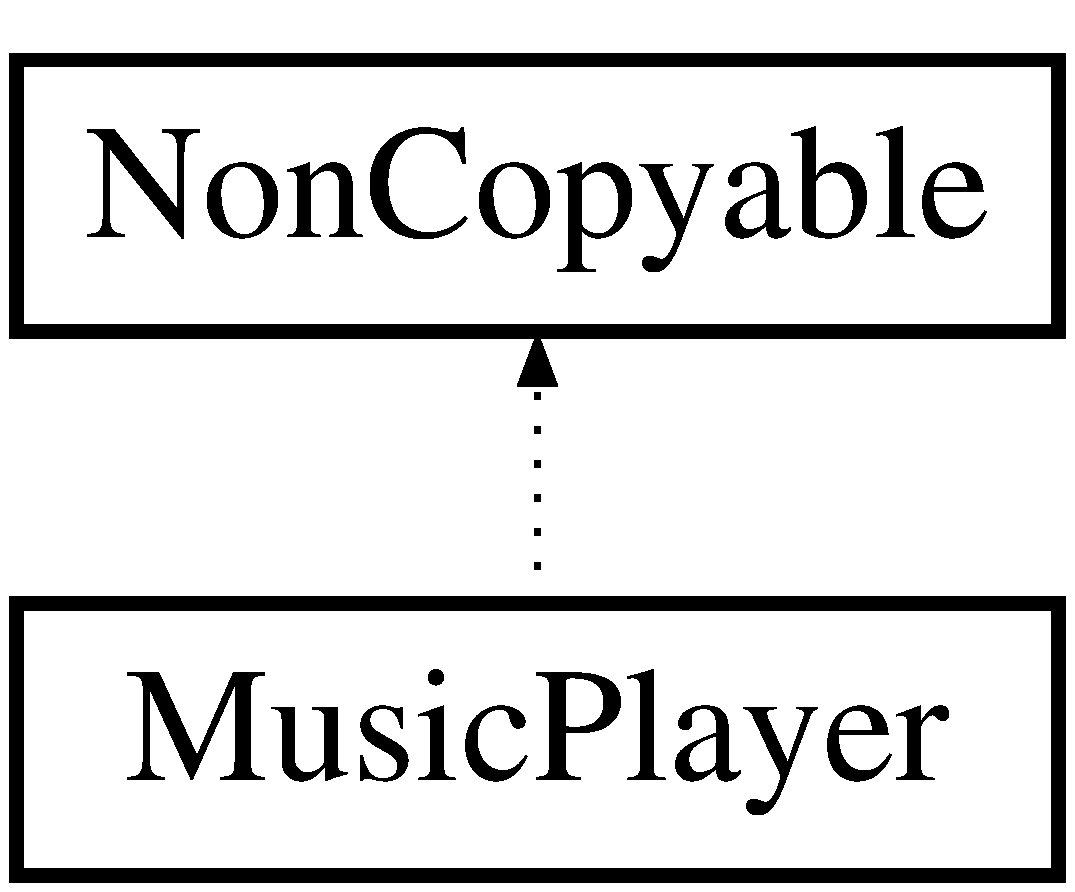
\includegraphics[height=2.000000cm]{classMusicPlayer}
\end{center}
\end{figure}
\subsection*{Métodos públicos}
\begin{DoxyCompactItemize}
\item 
\hyperlink{classMusicPlayer_a157211d92ff78fe87fdef2bb77a2b5fa}{Music\+Player} ()
\item 
void \hyperlink{classMusicPlayer_a47a4a1f9d2e2e3dcdc5fa4d252580d76}{play} (Music\+I\+D theme)
\item 
void \hyperlink{classMusicPlayer_a54e47a9e937730493d886aa5624c44d1}{stop} ()
\item 
void \hyperlink{classMusicPlayer_a59b313a9a9eb850e590f9c6555ad80cf}{set\+Paused} (bool paused)
\item 
void \hyperlink{classMusicPlayer_a361cbcbfb31d3c0c841d0b67a79c5cdd}{set\+Volume} (float volume)
\end{DoxyCompactItemize}


\subsection{Descripción detallada}
Reproductor de música 

\subsection{Documentación del constructor y destructor}
\hypertarget{classMusicPlayer_a157211d92ff78fe87fdef2bb77a2b5fa}{}\index{Music\+Player@{Music\+Player}!Music\+Player@{Music\+Player}}
\index{Music\+Player@{Music\+Player}!Music\+Player@{Music\+Player}}
\subsubsection[{Music\+Player}]{\setlength{\rightskip}{0pt plus 5cm}Music\+Player\+::\+Music\+Player (
\begin{DoxyParamCaption}
{}
\end{DoxyParamCaption}
)}\label{classMusicPlayer_a157211d92ff78fe87fdef2bb77a2b5fa}
Constructor 

\subsection{Documentación de las funciones miembro}
\hypertarget{classMusicPlayer_a47a4a1f9d2e2e3dcdc5fa4d252580d76}{}\index{Music\+Player@{Music\+Player}!play@{play}}
\index{play@{play}!Music\+Player@{Music\+Player}}
\subsubsection[{play}]{\setlength{\rightskip}{0pt plus 5cm}void Music\+Player\+::play (
\begin{DoxyParamCaption}
\item[{Music\+I\+D}]{theme}
\end{DoxyParamCaption}
)}\label{classMusicPlayer_a47a4a1f9d2e2e3dcdc5fa4d252580d76}
Reproduce la música del identificador dado 
\begin{DoxyParams}{Parámetros}
{\em theme} & identificador de la música \\
\hline
\end{DoxyParams}
\hypertarget{classMusicPlayer_a59b313a9a9eb850e590f9c6555ad80cf}{}\index{Music\+Player@{Music\+Player}!set\+Paused@{set\+Paused}}
\index{set\+Paused@{set\+Paused}!Music\+Player@{Music\+Player}}
\subsubsection[{set\+Paused}]{\setlength{\rightskip}{0pt plus 5cm}void Music\+Player\+::set\+Paused (
\begin{DoxyParamCaption}
\item[{bool}]{paused}
\end{DoxyParamCaption}
)}\label{classMusicPlayer_a59b313a9a9eb850e590f9c6555ad80cf}
Pausa o no la música 
\begin{DoxyParams}{Parámetros}
{\em paused} & true si se quiere pausar la música \\
\hline
\end{DoxyParams}
\hypertarget{classMusicPlayer_a361cbcbfb31d3c0c841d0b67a79c5cdd}{}\index{Music\+Player@{Music\+Player}!set\+Volume@{set\+Volume}}
\index{set\+Volume@{set\+Volume}!Music\+Player@{Music\+Player}}
\subsubsection[{set\+Volume}]{\setlength{\rightskip}{0pt plus 5cm}void Music\+Player\+::set\+Volume (
\begin{DoxyParamCaption}
\item[{float}]{volume}
\end{DoxyParamCaption}
)}\label{classMusicPlayer_a361cbcbfb31d3c0c841d0b67a79c5cdd}
Establece un volumen para la música 
\begin{DoxyParams}{Parámetros}
{\em volume} & \\
\hline
\end{DoxyParams}
\hypertarget{classMusicPlayer_a54e47a9e937730493d886aa5624c44d1}{}\index{Music\+Player@{Music\+Player}!stop@{stop}}
\index{stop@{stop}!Music\+Player@{Music\+Player}}
\subsubsection[{stop}]{\setlength{\rightskip}{0pt plus 5cm}void Music\+Player\+::stop (
\begin{DoxyParamCaption}
{}
\end{DoxyParamCaption}
)}\label{classMusicPlayer_a54e47a9e937730493d886aa5624c44d1}
Para la música 

La documentación para esta clase fue generada a partir de los siguientes ficheros\+:\begin{DoxyCompactItemize}
\item 
Music\+Player.\+h\item 
Music\+Player.\+cpp\end{DoxyCompactItemize}

\hypertarget{classObserver}{}\section{Referencia de la Clase Observer}
\label{classObserver}\index{Observer@{Observer}}


{\ttfamily \#include $<$Observer.\+h$>$}

Diagrama de herencias de Observer\begin{figure}[H]
\begin{center}
\leavevmode
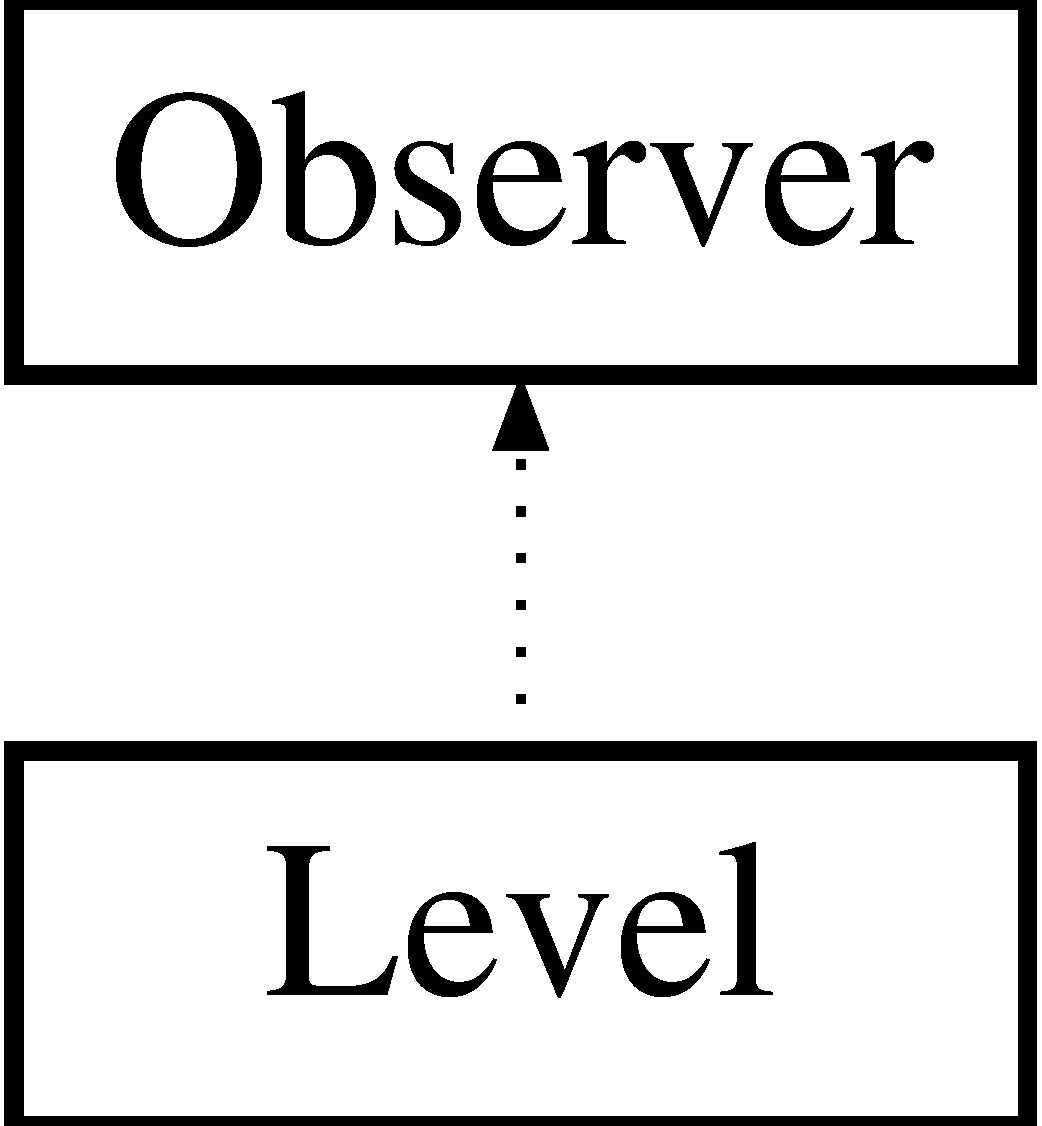
\includegraphics[height=2.000000cm]{classObserver}
\end{center}
\end{figure}
\subsection*{Métodos públicos}
\begin{DoxyCompactItemize}
\item 
int \hyperlink{classObserver_a0f330a29d7a3a7444fb79b6e4b59576d}{get\+Id} ()
\item 
\hyperlink{classObserver_a19c43f80a38a332a6f694783df3c9835}{Observer} ()
\item 
void \hyperlink{classObserver_a75bcfba81bc33d0b19ae1b33be1c9313}{set\+Subject} (\hyperlink{classSubject}{Subject} $\ast$mod)
\item 
virtual void \hyperlink{classObserver_ac75e4b339faeb3ea6fe0a01bf0b4a215}{update} ()=0
\end{DoxyCompactItemize}
\subsection*{Métodos protegidos}
\begin{DoxyCompactItemize}
\item 
\hyperlink{classSubject}{Subject} $\ast$ \hyperlink{classObserver_aa9de5b8862df591c9f63eb311ce1b70a}{get\+Subject} ()
\end{DoxyCompactItemize}


\subsection{Descripción detallada}
Observador del patrón observer 

\subsection{Documentación del constructor y destructor}
\hypertarget{classObserver_a19c43f80a38a332a6f694783df3c9835}{}\index{Observer@{Observer}!Observer@{Observer}}
\index{Observer@{Observer}!Observer@{Observer}}
\subsubsection[{Observer}]{\setlength{\rightskip}{0pt plus 5cm}Observer\+::\+Observer (
\begin{DoxyParamCaption}
{}
\end{DoxyParamCaption}
)\hspace{0.3cm}{\ttfamily [inline]}}\label{classObserver_a19c43f80a38a332a6f694783df3c9835}
Constructor 

\subsection{Documentación de las funciones miembro}
\hypertarget{classObserver_a0f330a29d7a3a7444fb79b6e4b59576d}{}\index{Observer@{Observer}!get\+Id@{get\+Id}}
\index{get\+Id@{get\+Id}!Observer@{Observer}}
\subsubsection[{get\+Id}]{\setlength{\rightskip}{0pt plus 5cm}int Observer\+::get\+Id (
\begin{DoxyParamCaption}
{}
\end{DoxyParamCaption}
)\hspace{0.3cm}{\ttfamily [inline]}}\label{classObserver_a0f330a29d7a3a7444fb79b6e4b59576d}
Devuelve el identificador del observador \begin{DoxyReturn}{Devuelve}
un número identificando al observador 
\end{DoxyReturn}
\hypertarget{classObserver_aa9de5b8862df591c9f63eb311ce1b70a}{}\index{Observer@{Observer}!get\+Subject@{get\+Subject}}
\index{get\+Subject@{get\+Subject}!Observer@{Observer}}
\subsubsection[{get\+Subject}]{\setlength{\rightskip}{0pt plus 5cm}{\bf Subject}$\ast$ Observer\+::get\+Subject (
\begin{DoxyParamCaption}
{}
\end{DoxyParamCaption}
)\hspace{0.3cm}{\ttfamily [inline]}, {\ttfamily [protected]}}\label{classObserver_aa9de5b8862df591c9f63eb311ce1b70a}
Devuelve el objeto vigilado \begin{DoxyReturn}{Devuelve}
objeto vigilado 
\end{DoxyReturn}
\hypertarget{classObserver_a75bcfba81bc33d0b19ae1b33be1c9313}{}\index{Observer@{Observer}!set\+Subject@{set\+Subject}}
\index{set\+Subject@{set\+Subject}!Observer@{Observer}}
\subsubsection[{set\+Subject}]{\setlength{\rightskip}{0pt plus 5cm}void Observer\+::set\+Subject (
\begin{DoxyParamCaption}
\item[{{\bf Subject} $\ast$}]{mod}
\end{DoxyParamCaption}
)}\label{classObserver_a75bcfba81bc33d0b19ae1b33be1c9313}
Setea el objeto a vigilar 
\begin{DoxyParams}{Parámetros}
{\em mod} & objeto a vigilar \\
\hline
\end{DoxyParams}
\hypertarget{classObserver_ac75e4b339faeb3ea6fe0a01bf0b4a215}{}\index{Observer@{Observer}!update@{update}}
\index{update@{update}!Observer@{Observer}}
\subsubsection[{update}]{\setlength{\rightskip}{0pt plus 5cm}virtual void Observer\+::update (
\begin{DoxyParamCaption}
{}
\end{DoxyParamCaption}
)\hspace{0.3cm}{\ttfamily [pure virtual]}}\label{classObserver_ac75e4b339faeb3ea6fe0a01bf0b4a215}
Método a ejecutar cuando haya cambios en el objeto vigilado 

Implementado en \hyperlink{classLevel_a62e412eaad753d2baa2f94239cb80e41}{Level}.



La documentación para esta clase fue generada a partir de los siguientes ficheros\+:\begin{DoxyCompactItemize}
\item 
Observer.\+h\item 
Observer.\+cpp\end{DoxyCompactItemize}

\hypertarget{structOnCollision}{}\section{Referencia de la Estructura On\+Collision}
\label{structOnCollision}\index{On\+Collision@{On\+Collision}}


{\ttfamily \#include $<$On\+Collision.\+h$>$}

\subsection*{Campos de datos}
\begin{DoxyCompactItemize}
\item 
std\+::function$<$ void(\hyperlink{structMessageCollision}{Message\+Collision} $\ast$message)$>$ \hyperlink{structOnCollision_ab2d10451b054b4a5306517de28d85903}{on\+Collision\+Function}
\end{DoxyCompactItemize}


\subsection{Descripción detallada}
Estructura de colisión en el que guarda una función a ejecutar 

\subsection{Documentación de los campos}
\hypertarget{structOnCollision_ab2d10451b054b4a5306517de28d85903}{}\index{On\+Collision@{On\+Collision}!on\+Collision\+Function@{on\+Collision\+Function}}
\index{on\+Collision\+Function@{on\+Collision\+Function}!On\+Collision@{On\+Collision}}
\subsubsection[{on\+Collision\+Function}]{\setlength{\rightskip}{0pt plus 5cm}std\+::function$<$void({\bf Message\+Collision}$\ast$ message)$>$ On\+Collision\+::on\+Collision\+Function}\label{structOnCollision_ab2d10451b054b4a5306517de28d85903}
Guarda una función que especifica un mensaje de colisión 

La documentación para esta estructura fue generada a partir del siguiente fichero\+:\begin{DoxyCompactItemize}
\item 
On\+Collision.\+h\end{DoxyCompactItemize}

\hypertarget{structOrderScene}{}\section{Referencia de la Estructura Order\+Scene}
\label{structOrderScene}\index{Order\+Scene@{Order\+Scene}}


{\ttfamily \#include $<$Scene\+Node.\+h$>$}

\subsection*{Métodos públicos}
\begin{DoxyCompactItemize}
\item 
\hypertarget{structOrderScene_ac42bf6120435a6876903266f3c598990}{}bool {\bfseries operator()} (const \hyperlink{classSceneNode}{Scene\+Node} $\ast$node1, const \hyperlink{classSceneNode}{Scene\+Node} $\ast$node2)\label{structOrderScene_ac42bf6120435a6876903266f3c598990}

\end{DoxyCompactItemize}


\subsection{Descripción detallada}
Estructura usada para el ordenamiento de los nodos 
\begin{DoxyParams}{Parámetros}
{\em node1} & \\
\hline
{\em node2} & \\
\hline
\end{DoxyParams}
\begin{DoxyReturn}{Devuelve}

\end{DoxyReturn}


La documentación para esta estructura fue generada a partir del siguiente fichero\+:\begin{DoxyCompactItemize}
\item 
Scene\+Node.\+h\end{DoxyCompactItemize}

\hypertarget{classParallelTask}{}\section{Referencia de la Clase Parallel\+Task}
\label{classParallelTask}\index{Parallel\+Task@{Parallel\+Task}}


{\ttfamily \#include $<$Parallel\+Task.\+h$>$}

Diagrama de herencias de Parallel\+Task\begin{figure}[H]
\begin{center}
\leavevmode
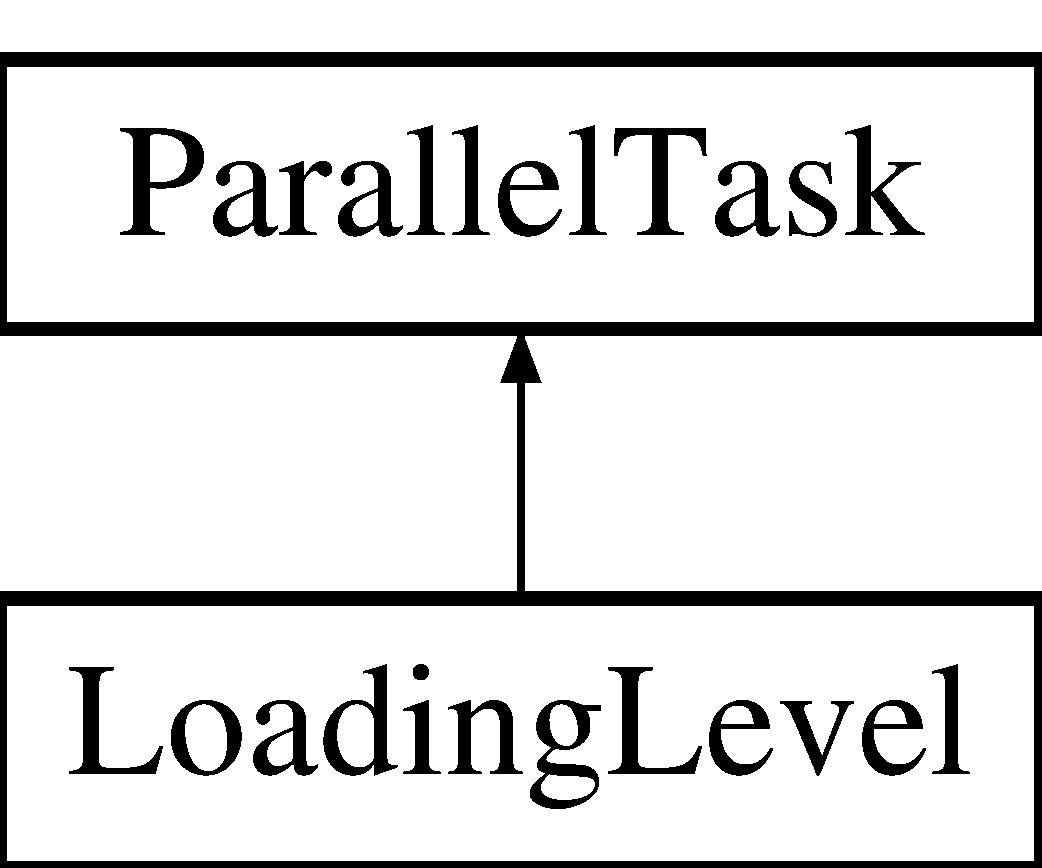
\includegraphics[height=2.000000cm]{classParallelTask}
\end{center}
\end{figure}
\subsection*{Métodos públicos}
\begin{DoxyCompactItemize}
\item 
\hyperlink{classParallelTask_a32cb3c361f7b4373f941f0993940576f}{Parallel\+Task} ()
\item 
\hypertarget{classParallelTask_ad1e7ba9134cc7961ab178a2f47cf54be}{}void {\bfseries execute} ()\label{classParallelTask_ad1e7ba9134cc7961ab178a2f47cf54be}

\item 
bool \hyperlink{classParallelTask_a1a67f547aa382fac2087184b2eb19148}{is\+Finished} ()
\item 
float \hyperlink{classParallelTask_ada45e4db1aa8a89f20ab0b8662c6dabc}{get\+Completion} ()
\item 
virtual \hyperlink{classParallelTask_aa0832c15ace4a003c1a9e617e48ccb17}{$\sim$\+Parallel\+Task} ()
\item 
virtual void \hyperlink{classParallelTask_a494412a04608d42f3ba91b1b242fd149}{run\+Task} ()=0
\end{DoxyCompactItemize}
\subsection*{Atributos protegidos}
\begin{DoxyCompactItemize}
\item 
sf\+::\+Thread \hyperlink{classParallelTask_a8ad7af10ec7f3e7fa84998111d280e97}{thread}
\item 
bool \hyperlink{classParallelTask_a924792685ebc2bd3bf8ec80e0dabe99f}{finished}
\item 
sf\+::\+Mutex \hyperlink{classParallelTask_a39d71d5f6fd7fe3de25452c147028c91}{mutex}
\item 
int \hyperlink{classParallelTask_a415d5be8b846af856f0a5b651711a4ad}{completion}
\end{DoxyCompactItemize}


\subsection{Descripción detallada}
Clase que realiza un trabajo en paralelo 

\subsection{Documentación del constructor y destructor}
\hypertarget{classParallelTask_a32cb3c361f7b4373f941f0993940576f}{}\index{Parallel\+Task@{Parallel\+Task}!Parallel\+Task@{Parallel\+Task}}
\index{Parallel\+Task@{Parallel\+Task}!Parallel\+Task@{Parallel\+Task}}
\subsubsection[{Parallel\+Task}]{\setlength{\rightskip}{0pt plus 5cm}Parallel\+Task\+::\+Parallel\+Task (
\begin{DoxyParamCaption}
{}
\end{DoxyParamCaption}
)}\label{classParallelTask_a32cb3c361f7b4373f941f0993940576f}
Constructor por defecto \hypertarget{classParallelTask_aa0832c15ace4a003c1a9e617e48ccb17}{}\index{Parallel\+Task@{Parallel\+Task}!````~Parallel\+Task@{$\sim$\+Parallel\+Task}}
\index{````~Parallel\+Task@{$\sim$\+Parallel\+Task}!Parallel\+Task@{Parallel\+Task}}
\subsubsection[{$\sim$\+Parallel\+Task}]{\setlength{\rightskip}{0pt plus 5cm}Parallel\+Task\+::$\sim$\+Parallel\+Task (
\begin{DoxyParamCaption}
{}
\end{DoxyParamCaption}
)\hspace{0.3cm}{\ttfamily [virtual]}}\label{classParallelTask_aa0832c15ace4a003c1a9e617e48ccb17}
Destructor 

\subsection{Documentación de las funciones miembro}
\hypertarget{classParallelTask_ada45e4db1aa8a89f20ab0b8662c6dabc}{}\index{Parallel\+Task@{Parallel\+Task}!get\+Completion@{get\+Completion}}
\index{get\+Completion@{get\+Completion}!Parallel\+Task@{Parallel\+Task}}
\subsubsection[{get\+Completion}]{\setlength{\rightskip}{0pt plus 5cm}float Parallel\+Task\+::get\+Completion (
\begin{DoxyParamCaption}
{}
\end{DoxyParamCaption}
)}\label{classParallelTask_ada45e4db1aa8a89f20ab0b8662c6dabc}
Devuelve un porcentaje \begin{DoxyReturn}{Devuelve}
porcentaje entre 0 y 1 
\end{DoxyReturn}
\hypertarget{classParallelTask_a1a67f547aa382fac2087184b2eb19148}{}\index{Parallel\+Task@{Parallel\+Task}!is\+Finished@{is\+Finished}}
\index{is\+Finished@{is\+Finished}!Parallel\+Task@{Parallel\+Task}}
\subsubsection[{is\+Finished}]{\setlength{\rightskip}{0pt plus 5cm}bool Parallel\+Task\+::is\+Finished (
\begin{DoxyParamCaption}
{}
\end{DoxyParamCaption}
)}\label{classParallelTask_a1a67f547aa382fac2087184b2eb19148}
Indica si ha terminado la tarea \begin{DoxyReturn}{Devuelve}
true si ha finalizado, false al contrario 
\end{DoxyReturn}
\hypertarget{classParallelTask_a494412a04608d42f3ba91b1b242fd149}{}\index{Parallel\+Task@{Parallel\+Task}!run\+Task@{run\+Task}}
\index{run\+Task@{run\+Task}!Parallel\+Task@{Parallel\+Task}}
\subsubsection[{run\+Task}]{\setlength{\rightskip}{0pt plus 5cm}virtual void Parallel\+Task\+::run\+Task (
\begin{DoxyParamCaption}
{}
\end{DoxyParamCaption}
)\hspace{0.3cm}{\ttfamily [pure virtual]}}\label{classParallelTask_a494412a04608d42f3ba91b1b242fd149}
Método a sobreescribir. En él se codifica la tarea a realizar 

Implementado en \hyperlink{classLoadingLevel_a14f8ce9f74732609e4da6c8cce387001}{Loading\+Level}.



\subsection{Documentación de los campos}
\hypertarget{classParallelTask_a415d5be8b846af856f0a5b651711a4ad}{}\index{Parallel\+Task@{Parallel\+Task}!completion@{completion}}
\index{completion@{completion}!Parallel\+Task@{Parallel\+Task}}
\subsubsection[{completion}]{\setlength{\rightskip}{0pt plus 5cm}int Parallel\+Task\+::completion\hspace{0.3cm}{\ttfamily [protected]}}\label{classParallelTask_a415d5be8b846af856f0a5b651711a4ad}
Number between 0 and 1 (percentaje of completion) \hypertarget{classParallelTask_a924792685ebc2bd3bf8ec80e0dabe99f}{}\index{Parallel\+Task@{Parallel\+Task}!finished@{finished}}
\index{finished@{finished}!Parallel\+Task@{Parallel\+Task}}
\subsubsection[{finished}]{\setlength{\rightskip}{0pt plus 5cm}bool Parallel\+Task\+::finished\hspace{0.3cm}{\ttfamily [protected]}}\label{classParallelTask_a924792685ebc2bd3bf8ec80e0dabe99f}
Variable para comprobar si la tarea ha terminado \hypertarget{classParallelTask_a39d71d5f6fd7fe3de25452c147028c91}{}\index{Parallel\+Task@{Parallel\+Task}!mutex@{mutex}}
\index{mutex@{mutex}!Parallel\+Task@{Parallel\+Task}}
\subsubsection[{mutex}]{\setlength{\rightskip}{0pt plus 5cm}sf\+::\+Mutex Parallel\+Task\+::mutex\hspace{0.3cm}{\ttfamily [protected]}}\label{classParallelTask_a39d71d5f6fd7fe3de25452c147028c91}
Semáforo para controlar datos entre más de un hilo \hypertarget{classParallelTask_a8ad7af10ec7f3e7fa84998111d280e97}{}\index{Parallel\+Task@{Parallel\+Task}!thread@{thread}}
\index{thread@{thread}!Parallel\+Task@{Parallel\+Task}}
\subsubsection[{thread}]{\setlength{\rightskip}{0pt plus 5cm}sf\+::\+Thread Parallel\+Task\+::thread\hspace{0.3cm}{\ttfamily [protected]}}\label{classParallelTask_a8ad7af10ec7f3e7fa84998111d280e97}
Hilo donde se ejecuta 

La documentación para esta clase fue generada a partir de los siguientes ficheros\+:\begin{DoxyCompactItemize}
\item 
Parallel\+Task.\+h\item 
Parallel\+Task.\+cpp\end{DoxyCompactItemize}

\hypertarget{classPartQuest}{}\section{Referencia de la Clase Part\+Quest}
\label{classPartQuest}\index{Part\+Quest@{Part\+Quest}}


{\ttfamily \#include $<$Part\+Quest.\+h$>$}

\subsection*{Métodos públicos}
\begin{DoxyCompactItemize}
\item 
\hyperlink{classPartQuest_a34beee72ffac9011bfe9297a24206734}{Part\+Quest} (Type\+Quest type, \hyperlink{classIdEntity}{Id\+Entity} destiny, \hyperlink{classIdEntity}{Id\+Entity} origin)
\item 
\hyperlink{classPartQuest_a95ff917dffd83bb251768845bd29d77f}{Part\+Quest} (Type\+Quest type, \hyperlink{classIdEntity}{Id\+Entity} destiny, \hyperlink{classIdEntity}{Id\+Entity} origin, Actions action)
\item 
\hyperlink{classPartQuest_a3c9f1f5534fe3873f7369e2c4c1ada6d}{Part\+Quest} (const \hyperlink{classPartQuest}{Part\+Quest} \&orig)
\item 
Actions \hyperlink{classPartQuest_a61047034367ebf891b764725ca2799d2}{get\+Action} () const 
\item 
void \hyperlink{classPartQuest_a27045fe31fafd738ea49457c1f776069}{set\+Action} (Actions action)
\item 
\hyperlink{classIdEntity}{Id\+Entity} \hyperlink{classPartQuest_a470d693e1e86d3705aae19fa1b77d7cf}{get\+Id\+Destiny} () const 
\item 
void \hyperlink{classPartQuest_ac2d0a47c74bfd5cc846e4ceda5547ca5}{set\+Id\+Destiny} (\hyperlink{classIdEntity}{Id\+Entity} id\+Destiny)
\item 
\hyperlink{classIdEntity}{Id\+Entity} \hyperlink{classPartQuest_a04d1b9b8e5a22bf18264981a621d8347}{get\+Id\+Origin} () const 
\item 
void \hyperlink{classPartQuest_ad72064f10d109cb51c62373ce563aa27}{set\+Id\+Origin} (\hyperlink{classIdEntity}{Id\+Entity} id\+Origin)
\item 
Type\+Quest \hyperlink{classPartQuest_a2bbac994710c6dc8b02dde2262d5ffe8}{get\+Type} () const 
\item 
void \hyperlink{classPartQuest_a14c9e56b0feed8a7453d19ed05a9e396}{set\+Type} (Type\+Quest type)
\item 
bool \hyperlink{classPartQuest_a922b2542a3ada799abb237a7f3cae518}{is\+Done} () const 
\item 
void \hyperlink{classPartQuest_adfded17b91e8e73ea8c2b21ea363dac1}{set\+Done} (bool done)
\end{DoxyCompactItemize}


\subsection{Descripción detallada}
Parte de una mision 

\subsection{Documentación del constructor y destructor}
\hypertarget{classPartQuest_a34beee72ffac9011bfe9297a24206734}{}\index{Part\+Quest@{Part\+Quest}!Part\+Quest@{Part\+Quest}}
\index{Part\+Quest@{Part\+Quest}!Part\+Quest@{Part\+Quest}}
\subsubsection[{Part\+Quest}]{\setlength{\rightskip}{0pt plus 5cm}Part\+Quest\+::\+Part\+Quest (
\begin{DoxyParamCaption}
\item[{Type\+Quest}]{type, }
\item[{{\bf Id\+Entity}}]{destiny, }
\item[{{\bf Id\+Entity}}]{origin}
\end{DoxyParamCaption}
)}\label{classPartQuest_a34beee72ffac9011bfe9297a24206734}
Constructor 
\begin{DoxyParams}{Parámetros}
{\em type} & tipo de mision \\
\hline
{\em destiny} & entidad de destino afectado \\
\hline
{\em origin} & entidad de origen afectado \\
\hline
\end{DoxyParams}
\hypertarget{classPartQuest_a95ff917dffd83bb251768845bd29d77f}{}\index{Part\+Quest@{Part\+Quest}!Part\+Quest@{Part\+Quest}}
\index{Part\+Quest@{Part\+Quest}!Part\+Quest@{Part\+Quest}}
\subsubsection[{Part\+Quest}]{\setlength{\rightskip}{0pt plus 5cm}Part\+Quest\+::\+Part\+Quest (
\begin{DoxyParamCaption}
\item[{Type\+Quest}]{type, }
\item[{{\bf Id\+Entity}}]{destiny, }
\item[{{\bf Id\+Entity}}]{origin, }
\item[{Actions}]{action}
\end{DoxyParamCaption}
)}\label{classPartQuest_a95ff917dffd83bb251768845bd29d77f}
Constructor 
\begin{DoxyParams}{Parámetros}
{\em type} & tipo de mision \\
\hline
{\em destiny} & entidad de destino afectado \\
\hline
{\em origin} & entidad de origen afectado \\
\hline
{\em action} & accion concreta cuando se especifica el tipo de mision A\+C\+T\+I\+O\+N \\
\hline
\end{DoxyParams}
\hypertarget{classPartQuest_a3c9f1f5534fe3873f7369e2c4c1ada6d}{}\index{Part\+Quest@{Part\+Quest}!Part\+Quest@{Part\+Quest}}
\index{Part\+Quest@{Part\+Quest}!Part\+Quest@{Part\+Quest}}
\subsubsection[{Part\+Quest}]{\setlength{\rightskip}{0pt plus 5cm}Part\+Quest\+::\+Part\+Quest (
\begin{DoxyParamCaption}
\item[{const {\bf Part\+Quest} \&}]{orig}
\end{DoxyParamCaption}
)}\label{classPartQuest_a3c9f1f5534fe3873f7369e2c4c1ada6d}
Constructor copia 
\begin{DoxyParams}{Parámetros}
{\em orig} & \\
\hline
\end{DoxyParams}


\subsection{Documentación de las funciones miembro}
\hypertarget{classPartQuest_a61047034367ebf891b764725ca2799d2}{}\index{Part\+Quest@{Part\+Quest}!get\+Action@{get\+Action}}
\index{get\+Action@{get\+Action}!Part\+Quest@{Part\+Quest}}
\subsubsection[{get\+Action}]{\setlength{\rightskip}{0pt plus 5cm}Actions Part\+Quest\+::get\+Action (
\begin{DoxyParamCaption}
{}
\end{DoxyParamCaption}
) const\hspace{0.3cm}{\ttfamily [inline]}}\label{classPartQuest_a61047034367ebf891b764725ca2799d2}
Devuelve la accion concreta \begin{DoxyReturn}{Devuelve}
accion 
\end{DoxyReturn}
\hypertarget{classPartQuest_a470d693e1e86d3705aae19fa1b77d7cf}{}\index{Part\+Quest@{Part\+Quest}!get\+Id\+Destiny@{get\+Id\+Destiny}}
\index{get\+Id\+Destiny@{get\+Id\+Destiny}!Part\+Quest@{Part\+Quest}}
\subsubsection[{get\+Id\+Destiny}]{\setlength{\rightskip}{0pt plus 5cm}{\bf Id\+Entity} Part\+Quest\+::get\+Id\+Destiny (
\begin{DoxyParamCaption}
{}
\end{DoxyParamCaption}
) const\hspace{0.3cm}{\ttfamily [inline]}}\label{classPartQuest_a470d693e1e86d3705aae19fa1b77d7cf}
Devuelve el id de la entidad destino afectada \begin{DoxyReturn}{Devuelve}
el id de la entidad destino afectada 
\end{DoxyReturn}
\hypertarget{classPartQuest_a04d1b9b8e5a22bf18264981a621d8347}{}\index{Part\+Quest@{Part\+Quest}!get\+Id\+Origin@{get\+Id\+Origin}}
\index{get\+Id\+Origin@{get\+Id\+Origin}!Part\+Quest@{Part\+Quest}}
\subsubsection[{get\+Id\+Origin}]{\setlength{\rightskip}{0pt plus 5cm}{\bf Id\+Entity} Part\+Quest\+::get\+Id\+Origin (
\begin{DoxyParamCaption}
{}
\end{DoxyParamCaption}
) const\hspace{0.3cm}{\ttfamily [inline]}}\label{classPartQuest_a04d1b9b8e5a22bf18264981a621d8347}
Devuelve el id de la entidad origen afectada \begin{DoxyReturn}{Devuelve}
el id de la entidad origen afectada 
\end{DoxyReturn}
\hypertarget{classPartQuest_a2bbac994710c6dc8b02dde2262d5ffe8}{}\index{Part\+Quest@{Part\+Quest}!get\+Type@{get\+Type}}
\index{get\+Type@{get\+Type}!Part\+Quest@{Part\+Quest}}
\subsubsection[{get\+Type}]{\setlength{\rightskip}{0pt plus 5cm}Type\+Quest Part\+Quest\+::get\+Type (
\begin{DoxyParamCaption}
{}
\end{DoxyParamCaption}
) const\hspace{0.3cm}{\ttfamily [inline]}}\label{classPartQuest_a2bbac994710c6dc8b02dde2262d5ffe8}
Devuelve el tipo de mision \begin{DoxyReturn}{Devuelve}
tipo de mision 
\end{DoxyReturn}
\hypertarget{classPartQuest_a922b2542a3ada799abb237a7f3cae518}{}\index{Part\+Quest@{Part\+Quest}!is\+Done@{is\+Done}}
\index{is\+Done@{is\+Done}!Part\+Quest@{Part\+Quest}}
\subsubsection[{is\+Done}]{\setlength{\rightskip}{0pt plus 5cm}bool Part\+Quest\+::is\+Done (
\begin{DoxyParamCaption}
{}
\end{DoxyParamCaption}
) const\hspace{0.3cm}{\ttfamily [inline]}}\label{classPartQuest_a922b2542a3ada799abb237a7f3cae518}
Indica si está hecho \begin{DoxyReturn}{Devuelve}
true si está hecho 
\end{DoxyReturn}
\hypertarget{classPartQuest_a27045fe31fafd738ea49457c1f776069}{}\index{Part\+Quest@{Part\+Quest}!set\+Action@{set\+Action}}
\index{set\+Action@{set\+Action}!Part\+Quest@{Part\+Quest}}
\subsubsection[{set\+Action}]{\setlength{\rightskip}{0pt plus 5cm}void Part\+Quest\+::set\+Action (
\begin{DoxyParamCaption}
\item[{Actions}]{action}
\end{DoxyParamCaption}
)\hspace{0.3cm}{\ttfamily [inline]}}\label{classPartQuest_a27045fe31fafd738ea49457c1f776069}
Setea la accion concreta que es cuando el tipo de mision es A\+C\+T\+I\+O\+N 
\begin{DoxyParams}{Parámetros}
{\em action} & \\
\hline
\end{DoxyParams}
\hypertarget{classPartQuest_adfded17b91e8e73ea8c2b21ea363dac1}{}\index{Part\+Quest@{Part\+Quest}!set\+Done@{set\+Done}}
\index{set\+Done@{set\+Done}!Part\+Quest@{Part\+Quest}}
\subsubsection[{set\+Done}]{\setlength{\rightskip}{0pt plus 5cm}void Part\+Quest\+::set\+Done (
\begin{DoxyParamCaption}
\item[{bool}]{done}
\end{DoxyParamCaption}
)\hspace{0.3cm}{\ttfamily [inline]}}\label{classPartQuest_adfded17b91e8e73ea8c2b21ea363dac1}
Setea si la parte de misión está hecha 
\begin{DoxyParams}{Parámetros}
{\em done} & true si está hecho \\
\hline
\end{DoxyParams}
\hypertarget{classPartQuest_ac2d0a47c74bfd5cc846e4ceda5547ca5}{}\index{Part\+Quest@{Part\+Quest}!set\+Id\+Destiny@{set\+Id\+Destiny}}
\index{set\+Id\+Destiny@{set\+Id\+Destiny}!Part\+Quest@{Part\+Quest}}
\subsubsection[{set\+Id\+Destiny}]{\setlength{\rightskip}{0pt plus 5cm}void Part\+Quest\+::set\+Id\+Destiny (
\begin{DoxyParamCaption}
\item[{{\bf Id\+Entity}}]{id\+Destiny}
\end{DoxyParamCaption}
)\hspace{0.3cm}{\ttfamily [inline]}}\label{classPartQuest_ac2d0a47c74bfd5cc846e4ceda5547ca5}
Setea el id de la entidad destino afectada 
\begin{DoxyParams}{Parámetros}
{\em id\+Destiny} & el id de la entidad destino afectada \\
\hline
\end{DoxyParams}
\hypertarget{classPartQuest_ad72064f10d109cb51c62373ce563aa27}{}\index{Part\+Quest@{Part\+Quest}!set\+Id\+Origin@{set\+Id\+Origin}}
\index{set\+Id\+Origin@{set\+Id\+Origin}!Part\+Quest@{Part\+Quest}}
\subsubsection[{set\+Id\+Origin}]{\setlength{\rightskip}{0pt plus 5cm}void Part\+Quest\+::set\+Id\+Origin (
\begin{DoxyParamCaption}
\item[{{\bf Id\+Entity}}]{id\+Origin}
\end{DoxyParamCaption}
)\hspace{0.3cm}{\ttfamily [inline]}}\label{classPartQuest_ad72064f10d109cb51c62373ce563aa27}
Setea el id de la entidad origen afectada 
\begin{DoxyParams}{Parámetros}
{\em id\+Origin} & el id de la entidad origen afectada \\
\hline
\end{DoxyParams}
\hypertarget{classPartQuest_a14c9e56b0feed8a7453d19ed05a9e396}{}\index{Part\+Quest@{Part\+Quest}!set\+Type@{set\+Type}}
\index{set\+Type@{set\+Type}!Part\+Quest@{Part\+Quest}}
\subsubsection[{set\+Type}]{\setlength{\rightskip}{0pt plus 5cm}void Part\+Quest\+::set\+Type (
\begin{DoxyParamCaption}
\item[{Type\+Quest}]{type}
\end{DoxyParamCaption}
)\hspace{0.3cm}{\ttfamily [inline]}}\label{classPartQuest_a14c9e56b0feed8a7453d19ed05a9e396}
Setea el tipo de mision 
\begin{DoxyParams}{Parámetros}
{\em type} & tipo de mision \\
\hline
\end{DoxyParams}


La documentación para esta clase fue generada a partir de los siguientes ficheros\+:\begin{DoxyCompactItemize}
\item 
Part\+Quest.\+h\item 
Part\+Quest.\+cpp\end{DoxyCompactItemize}

\hypertarget{classPauseState}{}\section{Referencia de la Clase Pause\+State}
\label{classPauseState}\index{Pause\+State@{Pause\+State}}


{\ttfamily \#include $<$Pause\+State.\+h$>$}

Diagrama de herencias de Pause\+State\begin{figure}[H]
\begin{center}
\leavevmode
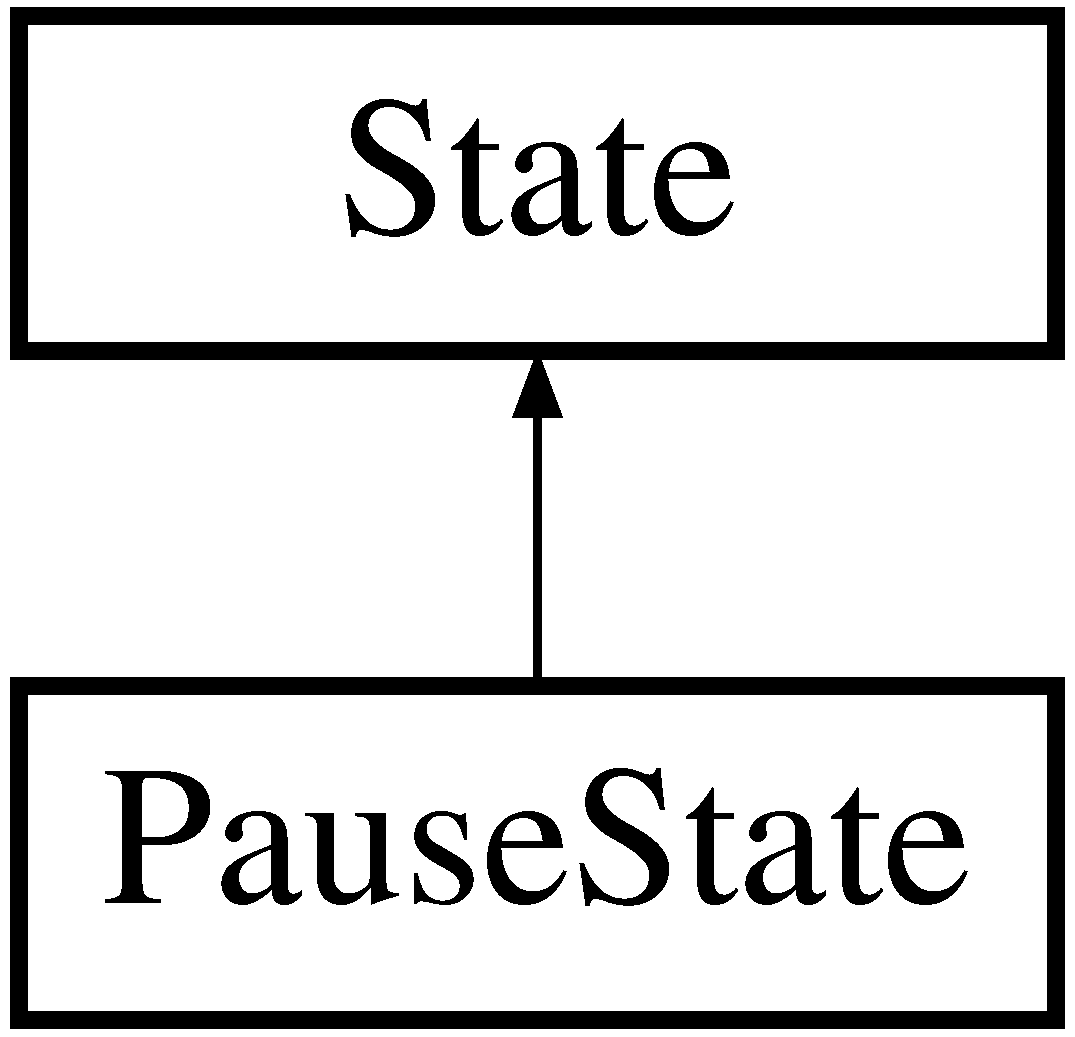
\includegraphics[height=2.000000cm]{classPauseState}
\end{center}
\end{figure}
\subsection*{Métodos públicos}
\begin{DoxyCompactItemize}
\item 
\hypertarget{classPauseState_a29710f2868096d4c7baccd7497f17a13}{}{\bfseries Pause\+State} (\hyperlink{classStateStack}{State\+Stack} \&\hyperlink{classState_a86c8d3a5a1ee89896828be85a785fb04}{stack}, \hyperlink{classContext}{Context} $\ast$\hyperlink{classState_adc93e8ad3199b5891618ca88eed0436a}{context})\label{classPauseState_a29710f2868096d4c7baccd7497f17a13}

\item 
virtual void \hyperlink{classPauseState_ac4c159c2f6d32eedd351f39e36c43f9d}{draw} ()
\item 
virtual bool \hyperlink{classPauseState_aed5aa4149e29b9124ade7a76a63941cd}{update} (sf\+::\+Time delta)
\item 
virtual bool \hyperlink{classPauseState_a685dda66dca3e1c41f4cb02da93c5a8d}{handle\+Event} (const sf\+::\+Event \&event)
\item 
virtual void \hyperlink{classPauseState_aa20ec5df0044a9652df788b9ad1aafb9}{pushed\+Action} ()
\item 
virtual void \hyperlink{classPauseState_ac04578f84a4c4fbcdf2d8b963b5f9fd0}{pulled\+Action} ()
\end{DoxyCompactItemize}
\subsection*{Otros miembros heredados}


\subsection{Descripción detallada}
Estado de pausa, muestra algunos botones 
\begin{DoxyParams}{Parámetros}
{\em stack} & \\
\hline
{\em context} & \\
\hline
\end{DoxyParams}


\subsection{Documentación de las funciones miembro}
\hypertarget{classPauseState_ac4c159c2f6d32eedd351f39e36c43f9d}{}\index{Pause\+State@{Pause\+State}!draw@{draw}}
\index{draw@{draw}!Pause\+State@{Pause\+State}}
\subsubsection[{draw}]{\setlength{\rightskip}{0pt plus 5cm}void Pause\+State\+::draw (
\begin{DoxyParamCaption}
{}
\end{DoxyParamCaption}
)\hspace{0.3cm}{\ttfamily [virtual]}}\label{classPauseState_ac4c159c2f6d32eedd351f39e36c43f9d}
Dibuja el estado 

Implementa \hyperlink{classState_ae261605bc40b7e3959ce5df5457e4942}{State}.

\hypertarget{classPauseState_a685dda66dca3e1c41f4cb02da93c5a8d}{}\index{Pause\+State@{Pause\+State}!handle\+Event@{handle\+Event}}
\index{handle\+Event@{handle\+Event}!Pause\+State@{Pause\+State}}
\subsubsection[{handle\+Event}]{\setlength{\rightskip}{0pt plus 5cm}bool Pause\+State\+::handle\+Event (
\begin{DoxyParamCaption}
\item[{const sf\+::\+Event \&}]{event}
\end{DoxyParamCaption}
)\hspace{0.3cm}{\ttfamily [virtual]}}\label{classPauseState_a685dda66dca3e1c41f4cb02da93c5a8d}
Procesa la entrada del usuario 
\begin{DoxyParams}{Parámetros}
{\em event} & evento \\
\hline
\end{DoxyParams}
\begin{DoxyReturn}{Devuelve}
true si lo ha procesado, false si no (o lo ha procesado pero que continúe) 
\end{DoxyReturn}


Implementa \hyperlink{classState_a19965f83460b248c42952aac8d001206}{State}.

\hypertarget{classPauseState_ac04578f84a4c4fbcdf2d8b963b5f9fd0}{}\index{Pause\+State@{Pause\+State}!pulled\+Action@{pulled\+Action}}
\index{pulled\+Action@{pulled\+Action}!Pause\+State@{Pause\+State}}
\subsubsection[{pulled\+Action}]{\setlength{\rightskip}{0pt plus 5cm}void Pause\+State\+::pulled\+Action (
\begin{DoxyParamCaption}
{}
\end{DoxyParamCaption}
)\hspace{0.3cm}{\ttfamily [virtual]}}\label{classPauseState_ac04578f84a4c4fbcdf2d8b963b5f9fd0}
Método ejecutado cuando es sacado de la pila 

Reimplementado de \hyperlink{classState_a92620c4648de675037b20ec59edb52a3}{State}.

\hypertarget{classPauseState_aa20ec5df0044a9652df788b9ad1aafb9}{}\index{Pause\+State@{Pause\+State}!pushed\+Action@{pushed\+Action}}
\index{pushed\+Action@{pushed\+Action}!Pause\+State@{Pause\+State}}
\subsubsection[{pushed\+Action}]{\setlength{\rightskip}{0pt plus 5cm}void Pause\+State\+::pushed\+Action (
\begin{DoxyParamCaption}
{}
\end{DoxyParamCaption}
)\hspace{0.3cm}{\ttfamily [virtual]}}\label{classPauseState_aa20ec5df0044a9652df788b9ad1aafb9}
Método ejecutado cuando es puesto en pila 

Reimplementado de \hyperlink{classState_a3cc6a1378f32f9ed6a2d1d8140296808}{State}.

\hypertarget{classPauseState_aed5aa4149e29b9124ade7a76a63941cd}{}\index{Pause\+State@{Pause\+State}!update@{update}}
\index{update@{update}!Pause\+State@{Pause\+State}}
\subsubsection[{update}]{\setlength{\rightskip}{0pt plus 5cm}bool Pause\+State\+::update (
\begin{DoxyParamCaption}
\item[{sf\+::\+Time}]{delta}
\end{DoxyParamCaption}
)\hspace{0.3cm}{\ttfamily [virtual]}}\label{classPauseState_aed5aa4149e29b9124ade7a76a63941cd}
Actualiza el estado 
\begin{DoxyParams}{Parámetros}
{\em delta} & tiempo entre frame y frame \\
\hline
\end{DoxyParams}
\begin{DoxyReturn}{Devuelve}
true si se ha actualizado 
\end{DoxyReturn}


Implementa \hyperlink{classState_aa6366828eb50639e86b94008cfad9c5d}{State}.



La documentación para esta clase fue generada a partir de los siguientes ficheros\+:\begin{DoxyCompactItemize}
\item 
Pause\+State.\+h\item 
Pause\+State.\+cpp\end{DoxyCompactItemize}

\hypertarget{structPendingChange}{}\section{Referencia de la Estructura Pending\+Change}
\label{structPendingChange}\index{Pending\+Change@{Pending\+Change}}


{\ttfamily \#include $<$Pending\+Change.\+h$>$}

\subsection*{Métodos públicos}
\begin{DoxyCompactItemize}
\item 
\hyperlink{structPendingChange_a61fb7f911e961d1e63a26ff92cc395e8}{Pending\+Change} (Action\+Stack \hyperlink{structPendingChange_afa46a2cd704ab8d14aabdceb2270e012}{action}, States\+I\+D \hyperlink{structPendingChange_ae91440b55b46e766b964b0c8fa08abdb}{state\+I\+D}=States\+I\+D\+::\+None)
\end{DoxyCompactItemize}
\subsection*{Campos de datos}
\begin{DoxyCompactItemize}
\item 
Action\+Stack \hyperlink{structPendingChange_afa46a2cd704ab8d14aabdceb2270e012}{action}
\item 
States\+I\+D \hyperlink{structPendingChange_ae91440b55b46e766b964b0c8fa08abdb}{state\+I\+D}
\end{DoxyCompactItemize}


\subsection{Descripción detallada}
Estructura para guardar los cambios pendientes de hacer en la pila de estados 

\subsection{Documentación del constructor y destructor}
\hypertarget{structPendingChange_a61fb7f911e961d1e63a26ff92cc395e8}{}\index{Pending\+Change@{Pending\+Change}!Pending\+Change@{Pending\+Change}}
\index{Pending\+Change@{Pending\+Change}!Pending\+Change@{Pending\+Change}}
\subsubsection[{Pending\+Change}]{\setlength{\rightskip}{0pt plus 5cm}Pending\+Change\+::\+Pending\+Change (
\begin{DoxyParamCaption}
\item[{Action\+Stack}]{action, }
\item[{States\+I\+D}]{state\+I\+D = {\ttfamily StatesID\+:\+:None}}
\end{DoxyParamCaption}
)}\label{structPendingChange_a61fb7f911e961d1e63a26ff92cc395e8}
Constructor 
\begin{DoxyParams}{Parámetros}
{\em action} & sacar, limpiar, meter estado... \\
\hline
{\em state\+I\+D} & identificador del estado. Por defecto ninguno \\
\hline
\end{DoxyParams}


\subsection{Documentación de los campos}
\hypertarget{structPendingChange_afa46a2cd704ab8d14aabdceb2270e012}{}\index{Pending\+Change@{Pending\+Change}!action@{action}}
\index{action@{action}!Pending\+Change@{Pending\+Change}}
\subsubsection[{action}]{\setlength{\rightskip}{0pt plus 5cm}Action\+Stack Pending\+Change\+::action}\label{structPendingChange_afa46a2cd704ab8d14aabdceb2270e012}
Acción a realizar \hypertarget{structPendingChange_ae91440b55b46e766b964b0c8fa08abdb}{}\index{Pending\+Change@{Pending\+Change}!state\+I\+D@{state\+I\+D}}
\index{state\+I\+D@{state\+I\+D}!Pending\+Change@{Pending\+Change}}
\subsubsection[{state\+I\+D}]{\setlength{\rightskip}{0pt plus 5cm}States\+I\+D Pending\+Change\+::state\+I\+D}\label{structPendingChange_ae91440b55b46e766b964b0c8fa08abdb}
Identificador del estado implicado 

La documentación para esta estructura fue generada a partir de los siguientes ficheros\+:\begin{DoxyCompactItemize}
\item 
Pending\+Change.\+h\item 
Pending\+Change.\+cpp\end{DoxyCompactItemize}

\hypertarget{classPlayer}{}\section{Referencia de la Clase Player}
\label{classPlayer}\index{Player@{Player}}
\subsection*{Métodos públicos}
\begin{DoxyCompactItemize}
\item 
\hyperlink{classPlayer_affe0cc3cb714f6deb4e62f0c0d3f1fd8}{Player} ()
\item 
virtual \hyperlink{classPlayer_a749d2c00e1fe0f5c2746f7505a58c062}{$\sim$\+Player} ()
\item 
void \hyperlink{classPlayer_ae54732ae250cab9b1a68914e613e6ac4}{initialize} (\hyperlink{classSystemManager}{System\+Manager} \&manager\+System, \hyperlink{classSoundPlayer}{Sound\+Player} $\ast$m\+Sound)
\item 
void \hyperlink{classPlayer_ac84a4e0b787f92bf773ccd0d0483f5b1}{handle\+Event} (const sf\+::\+Event \&event, \hyperlink{classCommandQueue}{Command\+Queue} \&commands)
\item 
void \hyperlink{classPlayer_ac520744c103fb38763c8856b4f158627}{handle\+Realtime\+Input} (\hyperlink{classCommandQueue}{Command\+Queue} \&commands)
\item 
void \hyperlink{classPlayer_adb77b4b92f7e7b81957bb36a0723b5b8}{assign\+Key} (Actions action, sf\+::\+Keyboard\+::\+Key key)
\item 
sf\+::\+Keyboard\+::\+Key \hyperlink{classPlayer_acc8c2726b9942264b946e1eb2d5a3300}{get\+Assigned\+Key} (Actions action) const 
\end{DoxyCompactItemize}


\subsection{Documentación del constructor y destructor}
\hypertarget{classPlayer_affe0cc3cb714f6deb4e62f0c0d3f1fd8}{}\index{Player@{Player}!Player@{Player}}
\index{Player@{Player}!Player@{Player}}
\subsubsection[{Player}]{\setlength{\rightskip}{0pt plus 5cm}Player\+::\+Player (
\begin{DoxyParamCaption}
{}
\end{DoxyParamCaption}
)}\label{classPlayer_affe0cc3cb714f6deb4e62f0c0d3f1fd8}
Constructor \hypertarget{classPlayer_a749d2c00e1fe0f5c2746f7505a58c062}{}\index{Player@{Player}!````~Player@{$\sim$\+Player}}
\index{````~Player@{$\sim$\+Player}!Player@{Player}}
\subsubsection[{$\sim$\+Player}]{\setlength{\rightskip}{0pt plus 5cm}Player\+::$\sim$\+Player (
\begin{DoxyParamCaption}
{}
\end{DoxyParamCaption}
)\hspace{0.3cm}{\ttfamily [virtual]}}\label{classPlayer_a749d2c00e1fe0f5c2746f7505a58c062}
Destructor 

\subsection{Documentación de las funciones miembro}
\hypertarget{classPlayer_adb77b4b92f7e7b81957bb36a0723b5b8}{}\index{Player@{Player}!assign\+Key@{assign\+Key}}
\index{assign\+Key@{assign\+Key}!Player@{Player}}
\subsubsection[{assign\+Key}]{\setlength{\rightskip}{0pt plus 5cm}void Player\+::assign\+Key (
\begin{DoxyParamCaption}
\item[{Actions}]{action, }
\item[{sf\+::\+Keyboard\+::\+Key}]{key}
\end{DoxyParamCaption}
)}\label{classPlayer_adb77b4b92f7e7b81957bb36a0723b5b8}
Asigna una tecla a una determinada acción 
\begin{DoxyParams}{Parámetros}
{\em action} & acción a setear \\
\hline
{\em key} & código de tecla asociada a la acción \\
\hline
\end{DoxyParams}
\hypertarget{classPlayer_acc8c2726b9942264b946e1eb2d5a3300}{}\index{Player@{Player}!get\+Assigned\+Key@{get\+Assigned\+Key}}
\index{get\+Assigned\+Key@{get\+Assigned\+Key}!Player@{Player}}
\subsubsection[{get\+Assigned\+Key}]{\setlength{\rightskip}{0pt plus 5cm}sf\+::\+Keyboard\+::\+Key Player\+::get\+Assigned\+Key (
\begin{DoxyParamCaption}
\item[{Actions}]{action}
\end{DoxyParamCaption}
) const}\label{classPlayer_acc8c2726b9942264b946e1eb2d5a3300}
Recupera la tecla asociada a una acción 
\begin{DoxyParams}{Parámetros}
{\em action} & acción consultada \\
\hline
\end{DoxyParams}
\begin{DoxyReturn}{Devuelve}
tecla asociada 
\end{DoxyReturn}
\hypertarget{classPlayer_ac84a4e0b787f92bf773ccd0d0483f5b1}{}\index{Player@{Player}!handle\+Event@{handle\+Event}}
\index{handle\+Event@{handle\+Event}!Player@{Player}}
\subsubsection[{handle\+Event}]{\setlength{\rightskip}{0pt plus 5cm}void Player\+::handle\+Event (
\begin{DoxyParamCaption}
\item[{const sf\+::\+Event \&}]{event, }
\item[{{\bf Command\+Queue} \&}]{commands}
\end{DoxyParamCaption}
)}\label{classPlayer_ac84a4e0b787f92bf773ccd0d0483f5b1}
Procesa la entrada, creando si es necesario un comando a ejecutar que deja en la pila de comandos 
\begin{DoxyParams}{Parámetros}
{\em event} & evento \\
\hline
{\em commands} & pila de comandos \\
\hline
\end{DoxyParams}
\hypertarget{classPlayer_ac520744c103fb38763c8856b4f158627}{}\index{Player@{Player}!handle\+Realtime\+Input@{handle\+Realtime\+Input}}
\index{handle\+Realtime\+Input@{handle\+Realtime\+Input}!Player@{Player}}
\subsubsection[{handle\+Realtime\+Input}]{\setlength{\rightskip}{0pt plus 5cm}void Player\+::handle\+Realtime\+Input (
\begin{DoxyParamCaption}
\item[{{\bf Command\+Queue} \&}]{commands}
\end{DoxyParamCaption}
)}\label{classPlayer_ac520744c103fb38763c8856b4f158627}
Procesa la entrada en tiempo real, creando si es necesario un comando a ejecutar que deja en la pila de comandos 
\begin{DoxyParams}{Parámetros}
{\em event} & evento \\
\hline
{\em commands} & pila de comandos \\
\hline
\end{DoxyParams}
\hypertarget{classPlayer_ae54732ae250cab9b1a68914e613e6ac4}{}\index{Player@{Player}!initialize@{initialize}}
\index{initialize@{initialize}!Player@{Player}}
\subsubsection[{initialize}]{\setlength{\rightskip}{0pt plus 5cm}void Player\+::initialize (
\begin{DoxyParamCaption}
\item[{{\bf System\+Manager} \&}]{manager\+System, }
\item[{{\bf Sound\+Player} $\ast$}]{m\+Sound}
\end{DoxyParamCaption}
)}\label{classPlayer_ae54732ae250cab9b1a68914e613e6ac4}
Inicializa el jugador, estableciendo la entrada a la que reacciona 
\begin{DoxyParams}{Parámetros}
{\em manager\+System} & gestor de sistemas del que pillará la información que necesite \\
\hline
{\em m\+Sound} & reproductor de sonidos para reproducir ante eventos \\
\hline
\end{DoxyParams}


La documentación para esta clase fue generada a partir de los siguientes ficheros\+:\begin{DoxyCompactItemize}
\item 
Player.\+h\item 
Player.\+cpp\end{DoxyCompactItemize}

\hypertarget{structPoint}{}\section{Referencia de la Estructura Point}
\label{structPoint}\index{Point@{Point}}


{\ttfamily \#include $<$Convex\+Hull.\+h$>$}

\subsection*{Métodos públicos}
\begin{DoxyCompactItemize}
\item 
\hypertarget{structPoint_a78b55e8d5466bb8c2cf60fa55f2562ff}{}{\bfseries Point} (double x, double y)\label{structPoint_a78b55e8d5466bb8c2cf60fa55f2562ff}

\item 
\hypertarget{structPoint_aa042f39cc8ef592350a152f407b15bce}{}bool {\bfseries operator$<$} (const \hyperlink{structPoint}{Point} \&p) const \label{structPoint_aa042f39cc8ef592350a152f407b15bce}

\end{DoxyCompactItemize}
\subsection*{Campos de datos}
\begin{DoxyCompactItemize}
\item 
\hypertarget{structPoint_ab99c56589bc8ad5fa5071387110a5bc7}{}double {\bfseries x}\label{structPoint_ab99c56589bc8ad5fa5071387110a5bc7}

\item 
\hypertarget{structPoint_afa38be143ae800e6ad69ce8ed4df62d8}{}double {\bfseries y}\label{structPoint_afa38be143ae800e6ad69ce8ed4df62d8}

\end{DoxyCompactItemize}


\subsection{Descripción detallada}
Implementation of Andrew\textquotesingle{}s monotone chain 2\+D convex hull algorithm. Asymptotic complexity\+: O(n log n). Practical performance\+: 0.\+5-\/1.\+0 seconds for n=1000000 on a 1\+G\+Hz machine. Definición de un punto en 2\+D 

La documentación para esta estructura fue generada a partir del siguiente fichero\+:\begin{DoxyCompactItemize}
\item 
Convex\+Hull.\+h\end{DoxyCompactItemize}

\hypertarget{classPosition}{}\section{Referencia de la Clase Position}
\label{classPosition}\index{Position@{Position}}
\subsection*{Métodos públicos}
\begin{DoxyCompactItemize}
\item 
\hypertarget{classPosition_a6520cead44f97c92f75a5ee7cb715ef2}{}{\bfseries Position} (\hyperlink{classPosition}{Position} \&other)\label{classPosition_a6520cead44f97c92f75a5ee7cb715ef2}

\item 
void \hyperlink{classPosition_a025b96aee195169c6a77deee64ae7e2f}{update\+Position} (float x, float y)
\item 
sf\+::\+Transformable \hyperlink{classPosition_acebed81105bf14b056411091f8295d9f}{get\+Position} () const 
\item 
void \hyperlink{classPosition_a9bae6fce3bc17a2afce6560fc17c5597}{set\+Position} (sf\+::\+Transformable position)
\item 
void \hyperlink{classPosition_ab8dfc7a537a0506c40772b5917f53989}{set\+Position} (float x, float y)
\item 
void \hyperlink{classPosition_ae79e4ed1b1685b69d17fb6821f265e0e}{set\+Position\+Increment} (float x, float y)
\item 
Cardinal\+Points \hyperlink{classPosition_ae0353c11bd8470d52b62837abfbb716a}{get\+Direction} ()
\end{DoxyCompactItemize}


\subsection{Documentación de las funciones miembro}
\hypertarget{classPosition_ae0353c11bd8470d52b62837abfbb716a}{}\index{Position@{Position}!get\+Direction@{get\+Direction}}
\index{get\+Direction@{get\+Direction}!Position@{Position}}
\subsubsection[{get\+Direction}]{\setlength{\rightskip}{0pt plus 5cm}Cardinal\+Points Position\+::get\+Direction (
\begin{DoxyParamCaption}
{}
\end{DoxyParamCaption}
)}\label{classPosition_ae0353c11bd8470d52b62837abfbb716a}
Comprueba con la posición anterior y determina hacia que dirección está mirando \begin{DoxyReturn}{Devuelve}
uno de los cuatro puntos cardinales hacia los que está mirando 
\end{DoxyReturn}
\hypertarget{classPosition_acebed81105bf14b056411091f8295d9f}{}\index{Position@{Position}!get\+Position@{get\+Position}}
\index{get\+Position@{get\+Position}!Position@{Position}}
\subsubsection[{get\+Position}]{\setlength{\rightskip}{0pt plus 5cm}sf\+::\+Transformable Position\+::get\+Position (
\begin{DoxyParamCaption}
{}
\end{DoxyParamCaption}
) const\hspace{0.3cm}{\ttfamily [inline]}}\label{classPosition_acebed81105bf14b056411091f8295d9f}
Devuelve la posición \begin{DoxyReturn}{Devuelve}
la posición 
\end{DoxyReturn}
\hypertarget{classPosition_a9bae6fce3bc17a2afce6560fc17c5597}{}\index{Position@{Position}!set\+Position@{set\+Position}}
\index{set\+Position@{set\+Position}!Position@{Position}}
\subsubsection[{set\+Position}]{\setlength{\rightskip}{0pt plus 5cm}void Position\+::set\+Position (
\begin{DoxyParamCaption}
\item[{sf\+::\+Transformable}]{position}
\end{DoxyParamCaption}
)\hspace{0.3cm}{\ttfamily [inline]}}\label{classPosition_a9bae6fce3bc17a2afce6560fc17c5597}
Setea una nueva posición y elimina la anterior (poniendo la misma posicion) 
\begin{DoxyParams}{Parámetros}
{\em position} & nueva posición \\
\hline
\end{DoxyParams}
\hypertarget{classPosition_ab8dfc7a537a0506c40772b5917f53989}{}\index{Position@{Position}!set\+Position@{set\+Position}}
\index{set\+Position@{set\+Position}!Position@{Position}}
\subsubsection[{set\+Position}]{\setlength{\rightskip}{0pt plus 5cm}void Position\+::set\+Position (
\begin{DoxyParamCaption}
\item[{float}]{x, }
\item[{float}]{y}
\end{DoxyParamCaption}
)\hspace{0.3cm}{\ttfamily [inline]}}\label{classPosition_ab8dfc7a537a0506c40772b5917f53989}
Setea una nueva posición y elimina la anterior (poniendo la misma posicion) 
\begin{DoxyParams}{Parámetros}
{\em x} & posición x \\
\hline
{\em y} & posición y \\
\hline
\end{DoxyParams}
\hypertarget{classPosition_ae79e4ed1b1685b69d17fb6821f265e0e}{}\index{Position@{Position}!set\+Position\+Increment@{set\+Position\+Increment}}
\index{set\+Position\+Increment@{set\+Position\+Increment}!Position@{Position}}
\subsubsection[{set\+Position\+Increment}]{\setlength{\rightskip}{0pt plus 5cm}void Position\+::set\+Position\+Increment (
\begin{DoxyParamCaption}
\item[{float}]{x, }
\item[{float}]{y}
\end{DoxyParamCaption}
)}\label{classPosition_ae79e4ed1b1685b69d17fb6821f265e0e}
Incrementa la posición y guarda la previa 
\begin{DoxyParams}{Parámetros}
{\em x} & incremento x \\
\hline
{\em y} & incremento y \\
\hline
\end{DoxyParams}
\hypertarget{classPosition_a025b96aee195169c6a77deee64ae7e2f}{}\index{Position@{Position}!update\+Position@{update\+Position}}
\index{update\+Position@{update\+Position}!Position@{Position}}
\subsubsection[{update\+Position}]{\setlength{\rightskip}{0pt plus 5cm}void Position\+::update\+Position (
\begin{DoxyParamCaption}
\item[{float}]{x, }
\item[{float}]{y}
\end{DoxyParamCaption}
)}\label{classPosition_a025b96aee195169c6a77deee64ae7e2f}
Normal update 
\begin{DoxyParams}{Parámetros}
{\em x} & \\
\hline
{\em y} & \\
\hline
\end{DoxyParams}


La documentación para esta clase fue generada a partir de los siguientes ficheros\+:\begin{DoxyCompactItemize}
\item 
Position.\+h\item 
Position.\+cpp\end{DoxyCompactItemize}

\hypertarget{classPropertyManager}{}\section{Referencia de la Clase Property\+Manager}
\label{classPropertyManager}\index{Property\+Manager@{Property\+Manager}}
Diagrama de herencias de Property\+Manager\begin{figure}[H]
\begin{center}
\leavevmode
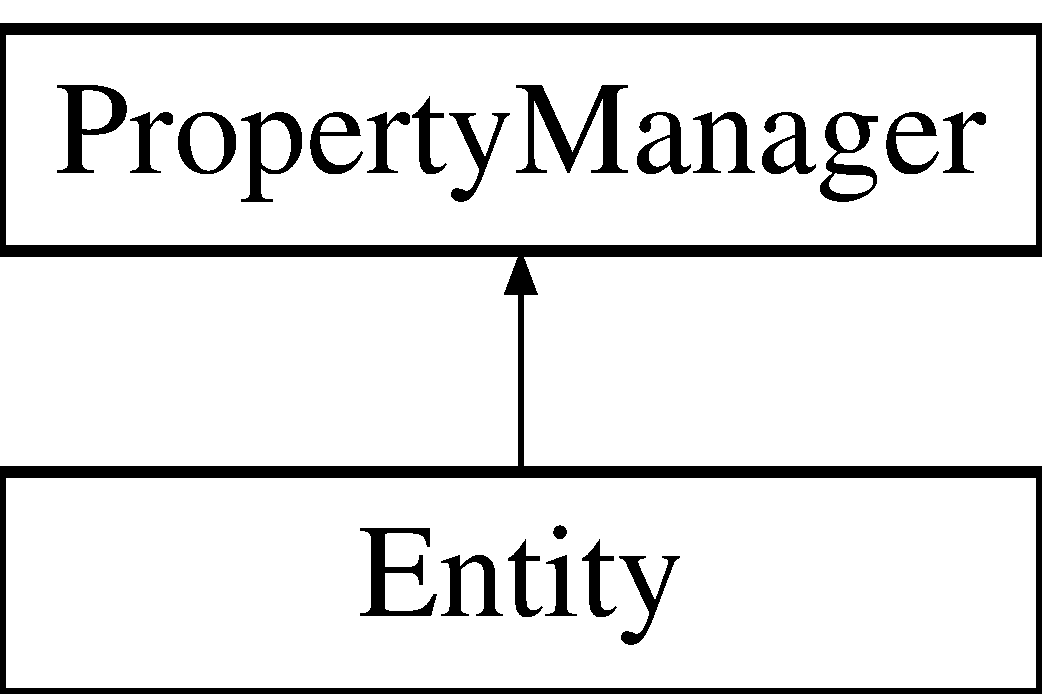
\includegraphics[height=2.000000cm]{classPropertyManager}
\end{center}
\end{figure}
\subsection*{Métodos públicos}
\begin{DoxyCompactItemize}
\item 
\hyperlink{classPropertyManager_a3b65b75bae28db832e98a38aec5774c6}{Property\+Manager} ()
\item 
virtual \hyperlink{classPropertyManager_aa16d7f0cb2a2baaa3b3afbe6239aac39}{$\sim$\+Property\+Manager} ()
\item 
bool \hyperlink{classPropertyManager_a36a6ba03a959d55810edb07740be3eba}{Has\+I\+D} (const std\+::string the\+Property\+I\+D)
\item 
{\footnotesize template$<$class T\+Y\+P\+E $>$ }\\T\+Y\+P\+E \hyperlink{classPropertyManager_aee3e23bbb59187ab2a9ecf7befdb0959}{Get} (const std\+::string the\+Property\+I\+D)
\item 
{\footnotesize template$<$class T\+Y\+P\+E $>$ }\\void \hyperlink{classPropertyManager_ab7ce7dda72b81fab5a96c8a13a619c75}{Set} (const std\+::string the\+Property\+I\+D, T\+Y\+P\+E the\+Value)
\item 
{\footnotesize template$<$class T\+Y\+P\+E $>$ }\\void \hyperlink{classPropertyManager_adbe08543c7c5a20fa86a0b67c45172c8}{Add} (const std\+::string the\+Property\+I\+D, T\+Y\+P\+E the\+Value)
\item 
void \hyperlink{classPropertyManager_af6509e575d0cd677daf63cb909ed91c8}{Add} (\hyperlink{classIProperty}{I\+Property} $\ast$the\+Property)
\item 
void \hyperlink{classPropertyManager_a77dc4b4617d344aff0481cd8e1cecb39}{Clone} (const \hyperlink{classPropertyManager}{Property\+Manager} \&the\+Property\+Manager)
\end{DoxyCompactItemize}


\subsection{Documentación del constructor y destructor}
\hypertarget{classPropertyManager_a3b65b75bae28db832e98a38aec5774c6}{}\index{Property\+Manager@{Property\+Manager}!Property\+Manager@{Property\+Manager}}
\index{Property\+Manager@{Property\+Manager}!Property\+Manager@{Property\+Manager}}
\subsubsection[{Property\+Manager}]{\setlength{\rightskip}{0pt plus 5cm}Property\+Manager\+::\+Property\+Manager (
\begin{DoxyParamCaption}
{}
\end{DoxyParamCaption}
)}\label{classPropertyManager_a3b65b75bae28db832e98a38aec5774c6}
\hyperlink{classPropertyManager}{Property\+Manager} default constructor \hypertarget{classPropertyManager_aa16d7f0cb2a2baaa3b3afbe6239aac39}{}\index{Property\+Manager@{Property\+Manager}!````~Property\+Manager@{$\sim$\+Property\+Manager}}
\index{````~Property\+Manager@{$\sim$\+Property\+Manager}!Property\+Manager@{Property\+Manager}}
\subsubsection[{$\sim$\+Property\+Manager}]{\setlength{\rightskip}{0pt plus 5cm}Property\+Manager\+::$\sim$\+Property\+Manager (
\begin{DoxyParamCaption}
{}
\end{DoxyParamCaption}
)\hspace{0.3cm}{\ttfamily [virtual]}}\label{classPropertyManager_aa16d7f0cb2a2baaa3b3afbe6239aac39}
\hyperlink{classPropertyManager}{Property\+Manager} deconstructor 

\subsection{Documentación de las funciones miembro}
\hypertarget{classPropertyManager_adbe08543c7c5a20fa86a0b67c45172c8}{}\index{Property\+Manager@{Property\+Manager}!Add@{Add}}
\index{Add@{Add}!Property\+Manager@{Property\+Manager}}
\subsubsection[{Add}]{\setlength{\rightskip}{0pt plus 5cm}template$<$class T\+Y\+P\+E $>$ void Property\+Manager\+::\+Add (
\begin{DoxyParamCaption}
\item[{const std\+::string}]{the\+Property\+I\+D, }
\item[{T\+Y\+P\+E}]{the\+Value}
\end{DoxyParamCaption}
)\hspace{0.3cm}{\ttfamily [inline]}}\label{classPropertyManager_adbe08543c7c5a20fa86a0b67c45172c8}
Add\+Property Creates a Property and addes it to this entity. 
\begin{DoxyParams}[1]{Parámetros}
\mbox{\tt in}  & {\em the\+Property\+I\+D} & is the I\+D of the property to create. \\
\hline
\mbox{\tt in}  & {\em the\+Value} & is the inital value to set. \\
\hline
\end{DoxyParams}
\hypertarget{classPropertyManager_af6509e575d0cd677daf63cb909ed91c8}{}\index{Property\+Manager@{Property\+Manager}!Add@{Add}}
\index{Add@{Add}!Property\+Manager@{Property\+Manager}}
\subsubsection[{Add}]{\setlength{\rightskip}{0pt plus 5cm}void Property\+Manager\+::\+Add (
\begin{DoxyParamCaption}
\item[{{\bf I\+Property} $\ast$}]{the\+Property}
\end{DoxyParamCaption}
)}\label{classPropertyManager_af6509e575d0cd677daf63cb909ed91c8}
Add\+Property gets a premade Property and addes it to this entity. 
\begin{DoxyParams}[1]{Parámetros}
\mbox{\tt in}  & {\em the\+Property} & is a pointer to a pre exisiting property. \\
\hline
\end{DoxyParams}
\hypertarget{classPropertyManager_a77dc4b4617d344aff0481cd8e1cecb39}{}\index{Property\+Manager@{Property\+Manager}!Clone@{Clone}}
\index{Clone@{Clone}!Property\+Manager@{Property\+Manager}}
\subsubsection[{Clone}]{\setlength{\rightskip}{0pt plus 5cm}void Property\+Manager\+::\+Clone (
\begin{DoxyParamCaption}
\item[{const {\bf Property\+Manager} \&}]{the\+Property\+Manager}
\end{DoxyParamCaption}
)}\label{classPropertyManager_a77dc4b4617d344aff0481cd8e1cecb39}
Clone is responsible for making a clone of each property in the \hyperlink{classPropertyManager}{Property\+Manager} provided. 
\begin{DoxyParams}[1]{Parámetros}
\mbox{\tt in}  & {\em the\+Property\+Manager} & to clone into ourselves \\
\hline
\end{DoxyParams}
\hypertarget{classPropertyManager_aee3e23bbb59187ab2a9ecf7befdb0959}{}\index{Property\+Manager@{Property\+Manager}!Get@{Get}}
\index{Get@{Get}!Property\+Manager@{Property\+Manager}}
\subsubsection[{Get}]{\setlength{\rightskip}{0pt plus 5cm}template$<$class T\+Y\+P\+E $>$ T\+Y\+P\+E Property\+Manager\+::\+Get (
\begin{DoxyParamCaption}
\item[{const std\+::string}]{the\+Property\+I\+D}
\end{DoxyParamCaption}
)\hspace{0.3cm}{\ttfamily [inline]}}\label{classPropertyManager_aee3e23bbb59187ab2a9ecf7befdb0959}
Get\+Property returns the property as type with the I\+D of the\+Property\+I\+D. 
\begin{DoxyParams}[1]{Parámetros}
\mbox{\tt in}  & {\em the\+Property\+I\+D} & is the I\+D of the property to return. \\
\hline
\end{DoxyParams}
\begin{DoxyReturn}{Devuelve}
the value stored in the found propery in the form of T\+Y\+P\+E. If no Property was found it returns the default value the type constructor. 
\end{DoxyReturn}
\hypertarget{classPropertyManager_a36a6ba03a959d55810edb07740be3eba}{}\index{Property\+Manager@{Property\+Manager}!Has\+I\+D@{Has\+I\+D}}
\index{Has\+I\+D@{Has\+I\+D}!Property\+Manager@{Property\+Manager}}
\subsubsection[{Has\+I\+D}]{\setlength{\rightskip}{0pt plus 5cm}bool Property\+Manager\+::\+Has\+I\+D (
\begin{DoxyParamCaption}
\item[{const std\+::string}]{the\+Property\+I\+D}
\end{DoxyParamCaption}
)}\label{classPropertyManager_a36a6ba03a959d55810edb07740be3eba}
Has\+Property returs true if the\+Property\+I\+D specified exists in this \hyperlink{classPropertyManager}{Property\+Manager}. 
\begin{DoxyParams}[1]{Parámetros}
\mbox{\tt in}  & {\em the\+Property\+I\+D} & to lookup in this \hyperlink{classPropertyManager}{Property\+Manager} \\
\hline
\end{DoxyParams}
\begin{DoxyReturn}{Devuelve}
true if the\+Property\+I\+D exists, false otherwise 
\end{DoxyReturn}
\hypertarget{classPropertyManager_ab7ce7dda72b81fab5a96c8a13a619c75}{}\index{Property\+Manager@{Property\+Manager}!Set@{Set}}
\index{Set@{Set}!Property\+Manager@{Property\+Manager}}
\subsubsection[{Set}]{\setlength{\rightskip}{0pt plus 5cm}template$<$class T\+Y\+P\+E $>$ void Property\+Manager\+::\+Set (
\begin{DoxyParamCaption}
\item[{const std\+::string}]{the\+Property\+I\+D, }
\item[{T\+Y\+P\+E}]{the\+Value}
\end{DoxyParamCaption}
)\hspace{0.3cm}{\ttfamily [inline]}}\label{classPropertyManager_ab7ce7dda72b81fab5a96c8a13a619c75}
Set\+Property sets the property with the I\+D of the\+Property\+I\+D to the\+Value. 
\begin{DoxyParams}[1]{Parámetros}
\mbox{\tt in}  & {\em the\+Property\+I\+D} & is the I\+D of the property to set. \\
\hline
\mbox{\tt in}  & {\em the\+Value} & is the value to set. \\
\hline
\end{DoxyParams}


La documentación para esta clase fue generada a partir de los siguientes ficheros\+:\begin{DoxyCompactItemize}
\item 
Property\+Manager.\+h\item 
Property\+Manager.\+cpp\end{DoxyCompactItemize}

\hypertarget{classQuadTree}{}\section{Referencia de la Clase Quad\+Tree}
\label{classQuadTree}\index{Quad\+Tree@{Quad\+Tree}}


{\ttfamily \#include $<$Quad\+Tree.\+h$>$}

\subsection*{Métodos públicos}
\begin{DoxyCompactItemize}
\item 
\hyperlink{classQuadTree_a96a9d7cbe65726a19c1d04ca590eaec0}{Quad\+Tree} (int level, sf\+::\+Int\+Rect bounds)
\item 
\hyperlink{classQuadTree_a4be1f4acd98d186e6da8de3ae7470514}{Quad\+Tree} (int level, sf\+::\+Float\+Rect bounds)
\item 
\hyperlink{classQuadTree_a2c195977908b54adde1296d95e190efa}{Quad\+Tree} (int level)
\item 
void \hyperlink{classQuadTree_a0c1976706b3dd28abd50efce4024b087}{clear} ()
\item 
void \hyperlink{classQuadTree_ae4e2555bfee54d85d918306d8588a29a}{insert} (\hyperlink{classEntity}{Entity} $\ast$object\+New, bool not\+Child=false)
\item 
bool \hyperlink{classQuadTree_afe0e6b1888d77e36fde30f394ed486ec}{remove} (\hyperlink{classEntity}{Entity} $\ast$object)
\item 
std\+::vector$<$ \hyperlink{classEntity}{Entity} $\ast$ $>$ $\ast$ \hyperlink{classQuadTree_a2ed00031c45ea4ea39719070ca962e5a}{retrieve} (std\+::vector$<$ \hyperlink{classEntity}{Entity} $\ast$ $>$ $\ast$list, \hyperlink{classEntity}{Entity} $\ast$object)
\item 
std\+::vector$<$ \hyperlink{classEntity}{Entity} $\ast$ $>$ $\ast$ \hyperlink{classQuadTree_a2b96dd59f214926f73c709c52909eb3c}{retrieve} (std\+::vector$<$ \hyperlink{classEntity}{Entity} $\ast$ $>$ $\ast$list, sf\+::\+Float\+Rect rect)
\item 
void \hyperlink{classQuadTree_acf6234d19444281325a3f5c248280779}{update} ()
\item 
void \hyperlink{classQuadTree_a8fbaf5f22c673ba6b2a71d4bad669867}{get\+Objects} (std\+::vector$<$ \hyperlink{classEntity}{Entity} $\ast$ $>$ \&list)
\item 
\hyperlink{classQuadTree}{Quad\+Tree} $\ast$ \hyperlink{classQuadTree_a794eee179f8ecee537f0309357924e41}{get\+Node\+Region} (sf\+::\+Float\+Rect region)
\item 
sf\+::\+Float\+Rect \hyperlink{classQuadTree_ad74d47d7e55b4e84de85329fe1678b0d}{get\+Bounds} () const 
\item 
void \hyperlink{classQuadTree_ad2e5a59504d9574e5095a42c1a35faea}{to\+String} ()
\end{DoxyCompactItemize}


\subsection{Descripción detallada}
Estructura de árbol cuaternario para estructurar por área los elementos colisionables El quadtree es un nodo del árbol 

\subsection{Documentación del constructor y destructor}
\hypertarget{classQuadTree_a96a9d7cbe65726a19c1d04ca590eaec0}{}\index{Quad\+Tree@{Quad\+Tree}!Quad\+Tree@{Quad\+Tree}}
\index{Quad\+Tree@{Quad\+Tree}!Quad\+Tree@{Quad\+Tree}}
\subsubsection[{Quad\+Tree}]{\setlength{\rightskip}{0pt plus 5cm}Quad\+Tree\+::\+Quad\+Tree (
\begin{DoxyParamCaption}
\item[{int}]{level, }
\item[{sf\+::\+Int\+Rect}]{bounds}
\end{DoxyParamCaption}
)}\label{classQuadTree_a96a9d7cbe65726a19c1d04ca590eaec0}
Crea un nodo de un determinado nivel y de una determinada área limitada 
\begin{DoxyParams}{Parámetros}
{\em level} & nivel \\
\hline
{\em bounds} & área que cubre el nodo \\
\hline
\end{DoxyParams}
\hypertarget{classQuadTree_a4be1f4acd98d186e6da8de3ae7470514}{}\index{Quad\+Tree@{Quad\+Tree}!Quad\+Tree@{Quad\+Tree}}
\index{Quad\+Tree@{Quad\+Tree}!Quad\+Tree@{Quad\+Tree}}
\subsubsection[{Quad\+Tree}]{\setlength{\rightskip}{0pt plus 5cm}Quad\+Tree\+::\+Quad\+Tree (
\begin{DoxyParamCaption}
\item[{int}]{level, }
\item[{sf\+::\+Float\+Rect}]{bounds}
\end{DoxyParamCaption}
)}\label{classQuadTree_a4be1f4acd98d186e6da8de3ae7470514}
Crea un nodo de un determinado nivel y de una determinada área limitada 
\begin{DoxyParams}{Parámetros}
{\em level} & nivel \\
\hline
{\em bounds} & área que cubre el nodo \\
\hline
\end{DoxyParams}
\hypertarget{classQuadTree_a2c195977908b54adde1296d95e190efa}{}\index{Quad\+Tree@{Quad\+Tree}!Quad\+Tree@{Quad\+Tree}}
\index{Quad\+Tree@{Quad\+Tree}!Quad\+Tree@{Quad\+Tree}}
\subsubsection[{Quad\+Tree}]{\setlength{\rightskip}{0pt plus 5cm}Quad\+Tree\+::\+Quad\+Tree (
\begin{DoxyParamCaption}
\item[{int}]{level}
\end{DoxyParamCaption}
)}\label{classQuadTree_a2c195977908b54adde1296d95e190efa}
Crea un nodo de un determinado nivel y sin especificar área 
\begin{DoxyParams}{Parámetros}
{\em level} & \\
\hline
\end{DoxyParams}


\subsection{Documentación de las funciones miembro}
\hypertarget{classQuadTree_a0c1976706b3dd28abd50efce4024b087}{}\index{Quad\+Tree@{Quad\+Tree}!clear@{clear}}
\index{clear@{clear}!Quad\+Tree@{Quad\+Tree}}
\subsubsection[{clear}]{\setlength{\rightskip}{0pt plus 5cm}void Quad\+Tree\+::clear (
\begin{DoxyParamCaption}
{}
\end{DoxyParamCaption}
)}\label{classQuadTree_a0c1976706b3dd28abd50efce4024b087}
Limpia el área \hypertarget{classQuadTree_ad74d47d7e55b4e84de85329fe1678b0d}{}\index{Quad\+Tree@{Quad\+Tree}!get\+Bounds@{get\+Bounds}}
\index{get\+Bounds@{get\+Bounds}!Quad\+Tree@{Quad\+Tree}}
\subsubsection[{get\+Bounds}]{\setlength{\rightskip}{0pt plus 5cm}sf\+::\+Float\+Rect Quad\+Tree\+::get\+Bounds (
\begin{DoxyParamCaption}
{}
\end{DoxyParamCaption}
) const\hspace{0.3cm}{\ttfamily [inline]}}\label{classQuadTree_ad74d47d7e55b4e84de85329fe1678b0d}
Devuelve los límites/región que contiene el nodo \begin{DoxyReturn}{Devuelve}
rectángulo con los límites de la región que contiene el nodo 
\end{DoxyReturn}
\hypertarget{classQuadTree_a794eee179f8ecee537f0309357924e41}{}\index{Quad\+Tree@{Quad\+Tree}!get\+Node\+Region@{get\+Node\+Region}}
\index{get\+Node\+Region@{get\+Node\+Region}!Quad\+Tree@{Quad\+Tree}}
\subsubsection[{get\+Node\+Region}]{\setlength{\rightskip}{0pt plus 5cm}{\bf Quad\+Tree} $\ast$ Quad\+Tree\+::get\+Node\+Region (
\begin{DoxyParamCaption}
\item[{sf\+::\+Float\+Rect}]{region}
\end{DoxyParamCaption}
)}\label{classQuadTree_a794eee179f8ecee537f0309357924e41}
Devuelve el nodo más profundo que contiene la región especificada 
\begin{DoxyParams}{Parámetros}
{\em region} & región consultada \\
\hline
\end{DoxyParams}
\begin{DoxyReturn}{Devuelve}
nodo que contiene la región o nullptr si no hay nodo que lo contenga 
\end{DoxyReturn}
\hypertarget{classQuadTree_a8fbaf5f22c673ba6b2a71d4bad669867}{}\index{Quad\+Tree@{Quad\+Tree}!get\+Objects@{get\+Objects}}
\index{get\+Objects@{get\+Objects}!Quad\+Tree@{Quad\+Tree}}
\subsubsection[{get\+Objects}]{\setlength{\rightskip}{0pt plus 5cm}void Quad\+Tree\+::get\+Objects (
\begin{DoxyParamCaption}
\item[{std\+::vector$<$ {\bf Entity} $\ast$ $>$ \&}]{list}
\end{DoxyParamCaption}
)}\label{classQuadTree_a8fbaf5f22c673ba6b2a71d4bad669867}
Devuelve las entidades del nodo y sus hijos 
\begin{DoxyParams}{Parámetros}
{\em list} & lista de entidades del subárbol a partir de este nodo \\
\hline
\end{DoxyParams}
\hypertarget{classQuadTree_ae4e2555bfee54d85d918306d8588a29a}{}\index{Quad\+Tree@{Quad\+Tree}!insert@{insert}}
\index{insert@{insert}!Quad\+Tree@{Quad\+Tree}}
\subsubsection[{insert}]{\setlength{\rightskip}{0pt plus 5cm}void Quad\+Tree\+::insert (
\begin{DoxyParamCaption}
\item[{{\bf Entity} $\ast$}]{object\+New, }
\item[{bool}]{not\+Child = {\ttfamily false}}
\end{DoxyParamCaption}
)}\label{classQuadTree_ae4e2555bfee54d85d918306d8588a29a}
Inserta una entidad. Si se permite y encaja mejor en algún nodo hijo, lo delega a los hijos. S\+I no encaja en el nodo y tiene padre, se lo pasa al padre 
\begin{DoxyParams}{Parámetros}
{\em object\+New} & entidad a guardar \\
\hline
{\em not\+Child} & por defecto false, permite que delege en el hijo si encaja mejor, true para no dar a los hijos \\
\hline
\end{DoxyParams}
\hypertarget{classQuadTree_afe0e6b1888d77e36fde30f394ed486ec}{}\index{Quad\+Tree@{Quad\+Tree}!remove@{remove}}
\index{remove@{remove}!Quad\+Tree@{Quad\+Tree}}
\subsubsection[{remove}]{\setlength{\rightskip}{0pt plus 5cm}bool Quad\+Tree\+::remove (
\begin{DoxyParamCaption}
\item[{{\bf Entity} $\ast$}]{object}
\end{DoxyParamCaption}
)}\label{classQuadTree_afe0e6b1888d77e36fde30f394ed486ec}
Elimina una entidad 
\begin{DoxyParams}{Parámetros}
{\em object} & entidad a eliminar \\
\hline
\end{DoxyParams}
\begin{DoxyReturn}{Devuelve}
true si se ha eliminado con éxito 
\end{DoxyReturn}
\hypertarget{classQuadTree_a2ed00031c45ea4ea39719070ca962e5a}{}\index{Quad\+Tree@{Quad\+Tree}!retrieve@{retrieve}}
\index{retrieve@{retrieve}!Quad\+Tree@{Quad\+Tree}}
\subsubsection[{retrieve}]{\setlength{\rightskip}{0pt plus 5cm}std\+::vector$<$ {\bf Entity} $\ast$ $>$ $\ast$ Quad\+Tree\+::retrieve (
\begin{DoxyParamCaption}
\item[{std\+::vector$<$ {\bf Entity} $\ast$ $>$ $\ast$}]{list, }
\item[{{\bf Entity} $\ast$}]{object}
\end{DoxyParamCaption}
)}\label{classQuadTree_a2ed00031c45ea4ea39719070ca962e5a}
Devuelve una lista de todas las entidades que colisionan con la entidad dada 
\begin{DoxyParams}{Parámetros}
{\em list} & lista donde guardar entidades colisionadas \\
\hline
{\em object} & entidad al que testear colisiones \\
\hline
\end{DoxyParams}
\begin{DoxyReturn}{Devuelve}
lista con las entidades que colisionan 
\end{DoxyReturn}
\hypertarget{classQuadTree_a2b96dd59f214926f73c709c52909eb3c}{}\index{Quad\+Tree@{Quad\+Tree}!retrieve@{retrieve}}
\index{retrieve@{retrieve}!Quad\+Tree@{Quad\+Tree}}
\subsubsection[{retrieve}]{\setlength{\rightskip}{0pt plus 5cm}std\+::vector$<$ {\bf Entity} $\ast$ $>$ $\ast$ Quad\+Tree\+::retrieve (
\begin{DoxyParamCaption}
\item[{std\+::vector$<$ {\bf Entity} $\ast$ $>$ $\ast$}]{list, }
\item[{sf\+::\+Float\+Rect}]{rect}
\end{DoxyParamCaption}
)}\label{classQuadTree_a2b96dd59f214926f73c709c52909eb3c}
Devuelve una lista de todas las entidades que están en la zona dada 
\begin{DoxyParams}{Parámetros}
{\em list} & lista donde guardar entidades de la zona \\
\hline
{\em rect} & zona a testear \\
\hline
\end{DoxyParams}
\begin{DoxyReturn}{Devuelve}
lista con las entidades que tocan la zona 
\end{DoxyReturn}
\hypertarget{classQuadTree_ad2e5a59504d9574e5095a42c1a35faea}{}\index{Quad\+Tree@{Quad\+Tree}!to\+String@{to\+String}}
\index{to\+String@{to\+String}!Quad\+Tree@{Quad\+Tree}}
\subsubsection[{to\+String}]{\setlength{\rightskip}{0pt plus 5cm}void Quad\+Tree\+::to\+String (
\begin{DoxyParamCaption}
{}
\end{DoxyParamCaption}
)}\label{classQuadTree_ad2e5a59504d9574e5095a42c1a35faea}
Imprime el árbol a partir de este nodo \hypertarget{classQuadTree_acf6234d19444281325a3f5c248280779}{}\index{Quad\+Tree@{Quad\+Tree}!update@{update}}
\index{update@{update}!Quad\+Tree@{Quad\+Tree}}
\subsubsection[{update}]{\setlength{\rightskip}{0pt plus 5cm}void Quad\+Tree\+::update (
\begin{DoxyParamCaption}
{}
\end{DoxyParamCaption}
)}\label{classQuadTree_acf6234d19444281325a3f5c248280779}
Actualiza el árbol, recolocando las entidades si es necesario 

La documentación para esta clase fue generada a partir de los siguientes ficheros\+:\begin{DoxyCompactItemize}
\item 
Quad\+Tree.\+h\item 
Quad\+Tree.\+cpp\end{DoxyCompactItemize}

\hypertarget{classQuest}{}\section{Referencia de la Clase Quest}
\label{classQuest}\index{Quest@{Quest}}


{\ttfamily \#include $<$Quest.\+h$>$}

\subsection*{Métodos públicos}
\begin{DoxyCompactItemize}
\item 
\hyperlink{classQuest_a61650b0aba1284905aa8ebd179b6d73d}{Quest} (int id, sf\+::\+String $\ast$text)
\item 
\hyperlink{classQuest_abbc3037881ba6cb3d7984308078bbc23}{Quest} (int id, sf\+::\+String $\ast$text, sf\+::\+Time time)
\item 
\hyperlink{classQuest_ab65f7c10c43586168876a74c5f4c054f}{Quest} (const \hyperlink{classQuest}{Quest} \&orig)
\item 
void \hyperlink{classQuest_af92871b6593c45a837e111826ee5ca25}{add\+Part\+Quest} (\hyperlink{classPartQuest}{Part\+Quest} $\ast$part)
\item 
sf\+::\+Time \hyperlink{classQuest_a1b5f2c8524f30a88214da003f41ad329}{get\+Time} () const 
\item 
void \hyperlink{classQuest_a68f13a90502307e82ac24112fda3ecde}{set\+Time} (sf\+::\+Time time)
\item 
sf\+::\+String $\ast$ \hyperlink{classQuest_af714e617eb99803a2e6459cb853cda00}{get\+Text} ()
\item 
bool \hyperlink{classQuest_ac6db87bb6ec663c16d38b67baceb10ff}{is\+Finished} ()
\item 
std\+::vector$<$ int $>$ \hyperlink{classQuest_af9233e7f9b5aa42038ba2244844d9700}{on\+Finished} ()
\item 
void \hyperlink{classQuest_a522c7653b498a7921afd6d4bb03120d9}{update} (sf\+::\+Time dt)
\item 
void \hyperlink{classQuest_a10eb74f76c110f71bf82dc5e8be4a446}{add\+Quest\+Open} (int id)
\item 
void \hyperlink{classQuest_ae4ec082cef55170dd6d8841cf2a4801d}{remove\+Quest\+Open} (int id)
\item 
int \hyperlink{classQuest_a4bc0819c3b54a86ed2c55be48486ed8b}{get\+Id} () const 
\item 
void \hyperlink{classQuest_af2667a3a83e8adc9ae1c5bd05ce4236e}{set\+Id} (int id)
\item 
bool \hyperlink{classQuest_ab95e89f2d91d40661dfd6c491de5d31d}{is\+Opened} () const 
\item 
void \hyperlink{classQuest_a142441b8eff8bf90cf67ccd0a9a253b9}{set\+Opened} (bool opened)
\item 
bool \hyperlink{classQuest_a79d362e6866de68e47e831892b090ea0}{is\+In\+Order} () const 
\item 
void \hyperlink{classQuest_ae25b1834eb58ae8db8088e2d73ccfa2c}{set\+In\+Order} (bool in\+Order)
\item 
const std\+::vector$<$ \hyperlink{classPartQuest}{Part\+Quest} $\ast$ $>$ \& \hyperlink{classQuest_a94b8c670af1427c533782e367b4e4c93}{get\+Part\+Quests} ()
\end{DoxyCompactItemize}


\subsection{Descripción detallada}
Representa una misión 

\subsection{Documentación del constructor y destructor}
\hypertarget{classQuest_a61650b0aba1284905aa8ebd179b6d73d}{}\index{Quest@{Quest}!Quest@{Quest}}
\index{Quest@{Quest}!Quest@{Quest}}
\subsubsection[{Quest}]{\setlength{\rightskip}{0pt plus 5cm}Quest\+::\+Quest (
\begin{DoxyParamCaption}
\item[{int}]{id, }
\item[{sf\+::\+String $\ast$}]{text}
\end{DoxyParamCaption}
)}\label{classQuest_a61650b0aba1284905aa8ebd179b6d73d}
Constructor para una misión sin limite de tiempo (tiempo=0) 
\begin{DoxyParams}{Parámetros}
{\em id} & identificador de la mision \\
\hline
{\em text} & texto descriptivo de la mision \\
\hline
\end{DoxyParams}
\hypertarget{classQuest_abbc3037881ba6cb3d7984308078bbc23}{}\index{Quest@{Quest}!Quest@{Quest}}
\index{Quest@{Quest}!Quest@{Quest}}
\subsubsection[{Quest}]{\setlength{\rightskip}{0pt plus 5cm}Quest\+::\+Quest (
\begin{DoxyParamCaption}
\item[{int}]{id, }
\item[{sf\+::\+String $\ast$}]{text, }
\item[{sf\+::\+Time}]{time}
\end{DoxyParamCaption}
)}\label{classQuest_abbc3037881ba6cb3d7984308078bbc23}
Constructor para una misión con limite de tiempo 
\begin{DoxyParams}{Parámetros}
{\em id} & identificador de la mision \\
\hline
{\em text} & texto descriptivo de la mision \\
\hline
{\em time} & el límite de tiempo para la mision. S\+I es 0, no hay límite \\
\hline
\end{DoxyParams}
\hypertarget{classQuest_ab65f7c10c43586168876a74c5f4c054f}{}\index{Quest@{Quest}!Quest@{Quest}}
\index{Quest@{Quest}!Quest@{Quest}}
\subsubsection[{Quest}]{\setlength{\rightskip}{0pt plus 5cm}Quest\+::\+Quest (
\begin{DoxyParamCaption}
\item[{const {\bf Quest} \&}]{orig}
\end{DoxyParamCaption}
)}\label{classQuest_ab65f7c10c43586168876a74c5f4c054f}
Constructor copia 
\begin{DoxyParams}{Parámetros}
{\em orig} & \\
\hline
\end{DoxyParams}


\subsection{Documentación de las funciones miembro}
\hypertarget{classQuest_af92871b6593c45a837e111826ee5ca25}{}\index{Quest@{Quest}!add\+Part\+Quest@{add\+Part\+Quest}}
\index{add\+Part\+Quest@{add\+Part\+Quest}!Quest@{Quest}}
\subsubsection[{add\+Part\+Quest}]{\setlength{\rightskip}{0pt plus 5cm}void Quest\+::add\+Part\+Quest (
\begin{DoxyParamCaption}
\item[{{\bf Part\+Quest} $\ast$}]{part}
\end{DoxyParamCaption}
)}\label{classQuest_af92871b6593c45a837e111826ee5ca25}
Añade una parte más a la mision 
\begin{DoxyParams}{Parámetros}
{\em part} & parte de mision \\
\hline
\end{DoxyParams}
\hypertarget{classQuest_a10eb74f76c110f71bf82dc5e8be4a446}{}\index{Quest@{Quest}!add\+Quest\+Open@{add\+Quest\+Open}}
\index{add\+Quest\+Open@{add\+Quest\+Open}!Quest@{Quest}}
\subsubsection[{add\+Quest\+Open}]{\setlength{\rightskip}{0pt plus 5cm}void Quest\+::add\+Quest\+Open (
\begin{DoxyParamCaption}
\item[{int}]{id}
\end{DoxyParamCaption}
)\hspace{0.3cm}{\ttfamily [inline]}}\label{classQuest_a10eb74f76c110f71bf82dc5e8be4a446}
Añade el identificador de una misión que se activará cuando esta misión termine 
\begin{DoxyParams}{Parámetros}
{\em id} & identificador de la mision que se activará \\
\hline
\end{DoxyParams}
\hypertarget{classQuest_a4bc0819c3b54a86ed2c55be48486ed8b}{}\index{Quest@{Quest}!get\+Id@{get\+Id}}
\index{get\+Id@{get\+Id}!Quest@{Quest}}
\subsubsection[{get\+Id}]{\setlength{\rightskip}{0pt plus 5cm}int Quest\+::get\+Id (
\begin{DoxyParamCaption}
{}
\end{DoxyParamCaption}
) const\hspace{0.3cm}{\ttfamily [inline]}}\label{classQuest_a4bc0819c3b54a86ed2c55be48486ed8b}
Devuelve el id de la mision \begin{DoxyReturn}{Devuelve}
id de la mision 
\end{DoxyReturn}
\hypertarget{classQuest_a94b8c670af1427c533782e367b4e4c93}{}\index{Quest@{Quest}!get\+Part\+Quests@{get\+Part\+Quests}}
\index{get\+Part\+Quests@{get\+Part\+Quests}!Quest@{Quest}}
\subsubsection[{get\+Part\+Quests}]{\setlength{\rightskip}{0pt plus 5cm}const std\+::vector$<${\bf Part\+Quest}$\ast$$>$\& Quest\+::get\+Part\+Quests (
\begin{DoxyParamCaption}
{}
\end{DoxyParamCaption}
)\hspace{0.3cm}{\ttfamily [inline]}}\label{classQuest_a94b8c670af1427c533782e367b4e4c93}
Devuelve las partes de la que consta la misión \begin{DoxyReturn}{Devuelve}
lista de partes de la mision 
\end{DoxyReturn}
\hypertarget{classQuest_af714e617eb99803a2e6459cb853cda00}{}\index{Quest@{Quest}!get\+Text@{get\+Text}}
\index{get\+Text@{get\+Text}!Quest@{Quest}}
\subsubsection[{get\+Text}]{\setlength{\rightskip}{0pt plus 5cm}sf\+::\+String$\ast$ Quest\+::get\+Text (
\begin{DoxyParamCaption}
{}
\end{DoxyParamCaption}
)\hspace{0.3cm}{\ttfamily [inline]}}\label{classQuest_af714e617eb99803a2e6459cb853cda00}
Devuelve la descripción de la mision \begin{DoxyReturn}{Devuelve}
descripcion de la mision 
\end{DoxyReturn}
\hypertarget{classQuest_a1b5f2c8524f30a88214da003f41ad329}{}\index{Quest@{Quest}!get\+Time@{get\+Time}}
\index{get\+Time@{get\+Time}!Quest@{Quest}}
\subsubsection[{get\+Time}]{\setlength{\rightskip}{0pt plus 5cm}sf\+::\+Time Quest\+::get\+Time (
\begin{DoxyParamCaption}
{}
\end{DoxyParamCaption}
) const\hspace{0.3cm}{\ttfamily [inline]}}\label{classQuest_a1b5f2c8524f30a88214da003f41ad329}
Devuelve el tiempo limite que dispone \begin{DoxyReturn}{Devuelve}
tiempo limite 
\end{DoxyReturn}
\hypertarget{classQuest_ac6db87bb6ec663c16d38b67baceb10ff}{}\index{Quest@{Quest}!is\+Finished@{is\+Finished}}
\index{is\+Finished@{is\+Finished}!Quest@{Quest}}
\subsubsection[{is\+Finished}]{\setlength{\rightskip}{0pt plus 5cm}bool Quest\+::is\+Finished (
\begin{DoxyParamCaption}
{}
\end{DoxyParamCaption}
)}\label{classQuest_ac6db87bb6ec663c16d38b67baceb10ff}
Indica si está finalizado \begin{DoxyReturn}{Devuelve}
true si esta finalizado 
\end{DoxyReturn}
\hypertarget{classQuest_a79d362e6866de68e47e831892b090ea0}{}\index{Quest@{Quest}!is\+In\+Order@{is\+In\+Order}}
\index{is\+In\+Order@{is\+In\+Order}!Quest@{Quest}}
\subsubsection[{is\+In\+Order}]{\setlength{\rightskip}{0pt plus 5cm}bool Quest\+::is\+In\+Order (
\begin{DoxyParamCaption}
{}
\end{DoxyParamCaption}
) const\hspace{0.3cm}{\ttfamily [inline]}}\label{classQuest_a79d362e6866de68e47e831892b090ea0}
Indica si las partes de la mision se hacen en orden o no \begin{DoxyReturn}{Devuelve}
true si las partes de la mision se tienen que hacer en orden 
\end{DoxyReturn}
\hypertarget{classQuest_ab95e89f2d91d40661dfd6c491de5d31d}{}\index{Quest@{Quest}!is\+Opened@{is\+Opened}}
\index{is\+Opened@{is\+Opened}!Quest@{Quest}}
\subsubsection[{is\+Opened}]{\setlength{\rightskip}{0pt plus 5cm}bool Quest\+::is\+Opened (
\begin{DoxyParamCaption}
{}
\end{DoxyParamCaption}
) const\hspace{0.3cm}{\ttfamily [inline]}}\label{classQuest_ab95e89f2d91d40661dfd6c491de5d31d}
Indica si la mision está activa \begin{DoxyReturn}{Devuelve}
true si esta activa/abierta 
\end{DoxyReturn}
\hypertarget{classQuest_af9233e7f9b5aa42038ba2244844d9700}{}\index{Quest@{Quest}!on\+Finished@{on\+Finished}}
\index{on\+Finished@{on\+Finished}!Quest@{Quest}}
\subsubsection[{on\+Finished}]{\setlength{\rightskip}{0pt plus 5cm}std\+::vector$<$ int $>$ Quest\+::on\+Finished (
\begin{DoxyParamCaption}
{}
\end{DoxyParamCaption}
)}\label{classQuest_af9233e7f9b5aa42038ba2244844d9700}
Lista de misiones que se activarán cuando esta mision se termine \begin{DoxyReturn}{Devuelve}
lista de misiones a activar al finalizar 
\end{DoxyReturn}
\hypertarget{classQuest_ae4ec082cef55170dd6d8841cf2a4801d}{}\index{Quest@{Quest}!remove\+Quest\+Open@{remove\+Quest\+Open}}
\index{remove\+Quest\+Open@{remove\+Quest\+Open}!Quest@{Quest}}
\subsubsection[{remove\+Quest\+Open}]{\setlength{\rightskip}{0pt plus 5cm}void Quest\+::remove\+Quest\+Open (
\begin{DoxyParamCaption}
\item[{int}]{id}
\end{DoxyParamCaption}
)\hspace{0.3cm}{\ttfamily [inline]}}\label{classQuest_ae4ec082cef55170dd6d8841cf2a4801d}
Elimina una misión dentro de las que se activan al finalizar esta mision 
\begin{DoxyParams}{Parámetros}
{\em id} & identificador de la mision a borrar \\
\hline
\end{DoxyParams}
\hypertarget{classQuest_af2667a3a83e8adc9ae1c5bd05ce4236e}{}\index{Quest@{Quest}!set\+Id@{set\+Id}}
\index{set\+Id@{set\+Id}!Quest@{Quest}}
\subsubsection[{set\+Id}]{\setlength{\rightskip}{0pt plus 5cm}void Quest\+::set\+Id (
\begin{DoxyParamCaption}
\item[{int}]{id}
\end{DoxyParamCaption}
)\hspace{0.3cm}{\ttfamily [inline]}}\label{classQuest_af2667a3a83e8adc9ae1c5bd05ce4236e}
Setea el id de la mision 
\begin{DoxyParams}{Parámetros}
{\em id} & id nueva de la mision \\
\hline
\end{DoxyParams}
\hypertarget{classQuest_ae25b1834eb58ae8db8088e2d73ccfa2c}{}\index{Quest@{Quest}!set\+In\+Order@{set\+In\+Order}}
\index{set\+In\+Order@{set\+In\+Order}!Quest@{Quest}}
\subsubsection[{set\+In\+Order}]{\setlength{\rightskip}{0pt plus 5cm}void Quest\+::set\+In\+Order (
\begin{DoxyParamCaption}
\item[{bool}]{in\+Order}
\end{DoxyParamCaption}
)\hspace{0.3cm}{\ttfamily [inline]}}\label{classQuest_ae25b1834eb58ae8db8088e2d73ccfa2c}
Setea si las partes de la mision se hacen en orden 
\begin{DoxyParams}{Parámetros}
{\em in\+Order} & true si se hacen en orden \\
\hline
\end{DoxyParams}
\hypertarget{classQuest_a142441b8eff8bf90cf67ccd0a9a253b9}{}\index{Quest@{Quest}!set\+Opened@{set\+Opened}}
\index{set\+Opened@{set\+Opened}!Quest@{Quest}}
\subsubsection[{set\+Opened}]{\setlength{\rightskip}{0pt plus 5cm}void Quest\+::set\+Opened (
\begin{DoxyParamCaption}
\item[{bool}]{opened}
\end{DoxyParamCaption}
)\hspace{0.3cm}{\ttfamily [inline]}}\label{classQuest_a142441b8eff8bf90cf67ccd0a9a253b9}
Setea si la mision esta activa 
\begin{DoxyParams}{Parámetros}
{\em opened} & true para activar la mision, false para dejarla inactiva \\
\hline
\end{DoxyParams}
\hypertarget{classQuest_a68f13a90502307e82ac24112fda3ecde}{}\index{Quest@{Quest}!set\+Time@{set\+Time}}
\index{set\+Time@{set\+Time}!Quest@{Quest}}
\subsubsection[{set\+Time}]{\setlength{\rightskip}{0pt plus 5cm}void Quest\+::set\+Time (
\begin{DoxyParamCaption}
\item[{sf\+::\+Time}]{time}
\end{DoxyParamCaption}
)\hspace{0.3cm}{\ttfamily [inline]}}\label{classQuest_a68f13a90502307e82ac24112fda3ecde}
Setea el tiempo limite 
\begin{DoxyParams}{Parámetros}
{\em time} & \\
\hline
\end{DoxyParams}
\hypertarget{classQuest_a522c7653b498a7921afd6d4bb03120d9}{}\index{Quest@{Quest}!update@{update}}
\index{update@{update}!Quest@{Quest}}
\subsubsection[{update}]{\setlength{\rightskip}{0pt plus 5cm}void Quest\+::update (
\begin{DoxyParamCaption}
\item[{sf\+::\+Time}]{dt}
\end{DoxyParamCaption}
)}\label{classQuest_a522c7653b498a7921afd6d4bb03120d9}
Actualiza la mision 
\begin{DoxyParams}{Parámetros}
{\em dt} & tiempo entre frame y frame \\
\hline
\end{DoxyParams}


La documentación para esta clase fue generada a partir de los siguientes ficheros\+:\begin{DoxyCompactItemize}
\item 
Quest.\+h\item 
Quest.\+cpp\end{DoxyCompactItemize}

\hypertarget{classQuestData}{}\section{Referencia de la Clase Quest\+Data}
\label{classQuestData}\index{Quest\+Data@{Quest\+Data}}


{\ttfamily \#include $<$Quest\+Data.\+h$>$}

\subsection*{Métodos públicos}
\begin{DoxyCompactItemize}
\item 
\hypertarget{classQuestData_a0ba8fcf790c42a18444ee458c4b2d8b0}{}{\bfseries Quest\+Data} (const \hyperlink{classQuestData}{Quest\+Data} \&orig)\label{classQuestData_a0ba8fcf790c42a18444ee458c4b2d8b0}

\end{DoxyCompactItemize}


\subsection{Descripción detallada}
Estructura para guardar información sobre misiones 

La documentación para esta clase fue generada a partir de los siguientes ficheros\+:\begin{DoxyCompactItemize}
\item 
Quest\+Data.\+h\item 
Quest\+Data.\+cpp\end{DoxyCompactItemize}

\hypertarget{classQuesteable}{}\section{Referencia de la Clase Questeable}
\label{classQuesteable}\index{Questeable@{Questeable}}


{\ttfamily \#include $<$Questeable.\+h$>$}

\subsection*{Métodos públicos}
\begin{DoxyCompactItemize}
\item 
\hyperlink{classQuesteable_a349fefa8b69a52de358c4d80361b2310}{Questeable} (int id)
\item 
\hypertarget{classQuesteable_a8af8a796336ee548f65d400e5fac6d86}{}{\bfseries Questeable} (const \hyperlink{classQuesteable}{Questeable} \&orig)\label{classQuesteable_a8af8a796336ee548f65d400e5fac6d86}

\item 
void \hyperlink{classQuesteable_a08b377eac63c8287697730937b2c16ee}{add\+Part\+Quest} (\hyperlink{classPartQuest}{Part\+Quest} $\ast$quest)
\item 
int \hyperlink{classQuesteable_aa2a3079c24b3ad0386e84a14d6ba1eea}{get\+Id\+Quest} () const 
\item 
const std\+::vector$<$ \hyperlink{classPartQuest}{Part\+Quest} $\ast$ $>$ \& \hyperlink{classQuesteable_aeee0993b9720f00fc1fb9bf7e7f87e09}{get\+Part\+Quest} ()
\end{DoxyCompactItemize}


\subsection{Descripción detallada}
Clase para la propiedad questeable 

\subsection{Documentación del constructor y destructor}
\hypertarget{classQuesteable_a349fefa8b69a52de358c4d80361b2310}{}\index{Questeable@{Questeable}!Questeable@{Questeable}}
\index{Questeable@{Questeable}!Questeable@{Questeable}}
\subsubsection[{Questeable}]{\setlength{\rightskip}{0pt plus 5cm}Questeable\+::\+Questeable (
\begin{DoxyParamCaption}
\item[{int}]{id}
\end{DoxyParamCaption}
)}\label{classQuesteable_a349fefa8b69a52de358c4d80361b2310}
Constructor 
\begin{DoxyParams}{Parámetros}
{\em id} & identificador de la misión \\
\hline
\end{DoxyParams}


\subsection{Documentación de las funciones miembro}
\hypertarget{classQuesteable_a08b377eac63c8287697730937b2c16ee}{}\index{Questeable@{Questeable}!add\+Part\+Quest@{add\+Part\+Quest}}
\index{add\+Part\+Quest@{add\+Part\+Quest}!Questeable@{Questeable}}
\subsubsection[{add\+Part\+Quest}]{\setlength{\rightskip}{0pt plus 5cm}void Questeable\+::add\+Part\+Quest (
\begin{DoxyParamCaption}
\item[{{\bf Part\+Quest} $\ast$}]{quest}
\end{DoxyParamCaption}
)}\label{classQuesteable_a08b377eac63c8287697730937b2c16ee}
Añade la parte de misión asociada 
\begin{DoxyParams}{Parámetros}
{\em quest} & parte de misión \\
\hline
\end{DoxyParams}
\hypertarget{classQuesteable_aa2a3079c24b3ad0386e84a14d6ba1eea}{}\index{Questeable@{Questeable}!get\+Id\+Quest@{get\+Id\+Quest}}
\index{get\+Id\+Quest@{get\+Id\+Quest}!Questeable@{Questeable}}
\subsubsection[{get\+Id\+Quest}]{\setlength{\rightskip}{0pt plus 5cm}int Questeable\+::get\+Id\+Quest (
\begin{DoxyParamCaption}
{}
\end{DoxyParamCaption}
) const\hspace{0.3cm}{\ttfamily [inline]}}\label{classQuesteable_aa2a3079c24b3ad0386e84a14d6ba1eea}
Devuelve el identificador de la misión \begin{DoxyReturn}{Devuelve}

\end{DoxyReturn}
\hypertarget{classQuesteable_aeee0993b9720f00fc1fb9bf7e7f87e09}{}\index{Questeable@{Questeable}!get\+Part\+Quest@{get\+Part\+Quest}}
\index{get\+Part\+Quest@{get\+Part\+Quest}!Questeable@{Questeable}}
\subsubsection[{get\+Part\+Quest}]{\setlength{\rightskip}{0pt plus 5cm}const std\+::vector$<${\bf Part\+Quest}$\ast$$>$\& Questeable\+::get\+Part\+Quest (
\begin{DoxyParamCaption}
{}
\end{DoxyParamCaption}
)\hspace{0.3cm}{\ttfamily [inline]}}\label{classQuesteable_aeee0993b9720f00fc1fb9bf7e7f87e09}
Devuelve la lista de partes de misión asociadas \begin{DoxyReturn}{Devuelve}

\end{DoxyReturn}


La documentación para esta clase fue generada a partir de los siguientes ficheros\+:\begin{DoxyCompactItemize}
\item 
Questeable.\+h\item 
Questeable.\+cpp\end{DoxyCompactItemize}

\hypertarget{classQuestState}{}\section{Referencia de la Clase Quest\+State}
\label{classQuestState}\index{Quest\+State@{Quest\+State}}


{\ttfamily \#include $<$Quest\+State.\+h$>$}

Diagrama de herencias de Quest\+State\begin{figure}[H]
\begin{center}
\leavevmode
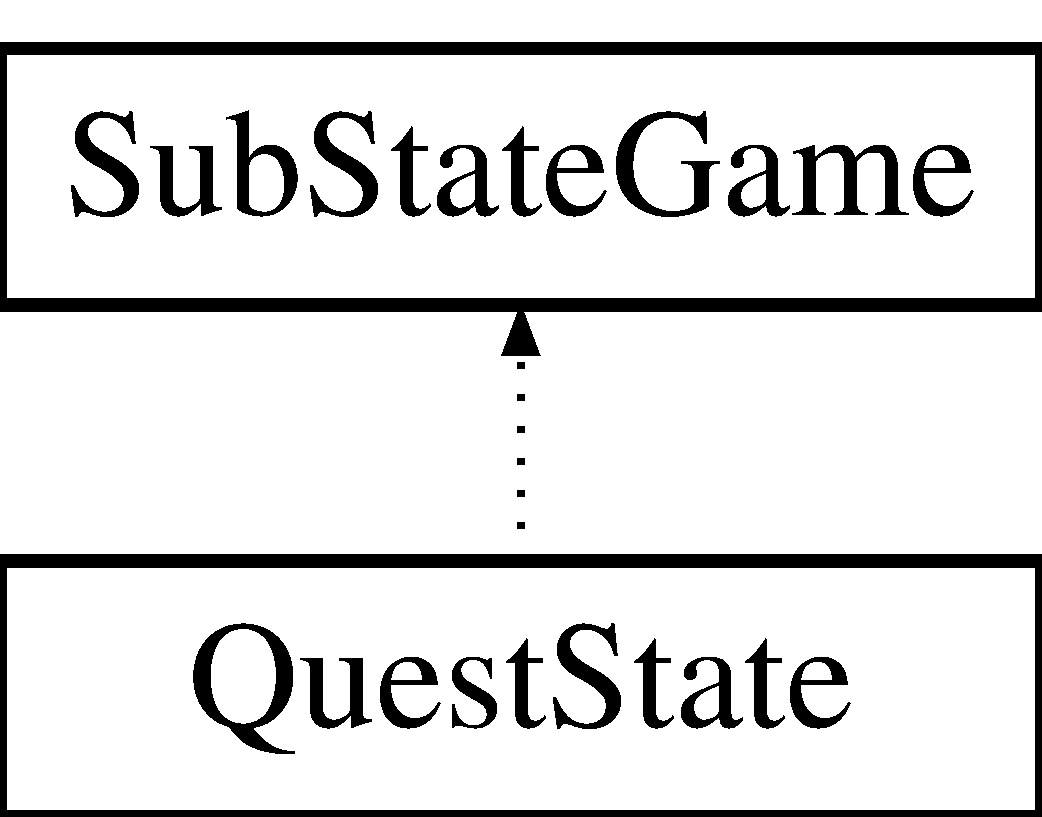
\includegraphics[height=2.000000cm]{classQuestState}
\end{center}
\end{figure}
\subsection*{Métodos públicos}
\begin{DoxyCompactItemize}
\item 
\hyperlink{classQuestState_a58f756d54bcb3717842ddf780eb02ca6}{Quest\+State} (\hyperlink{classSystemManager}{System\+Manager} $\ast$system)
\item 
\hypertarget{classQuestState_a7f8e3edcd9a531222f18472d686afb13}{}virtual void {\bfseries draw} ()\label{classQuestState_a7f8e3edcd9a531222f18472d686afb13}

\item 
\hypertarget{classQuestState_a5d13af2c97616fc55c278e6ed39bfad0}{}virtual bool {\bfseries update} (sf\+::\+Time delta)\label{classQuestState_a5d13af2c97616fc55c278e6ed39bfad0}

\item 
\hypertarget{classQuestState_acebc27cba666647c840cb928a1e6474c}{}virtual bool {\bfseries handle\+Event} (const sf\+::\+Event \&event)\label{classQuestState_acebc27cba666647c840cb928a1e6474c}

\end{DoxyCompactItemize}


\subsection{Descripción detallada}
Subestado para las misiones 

\subsection{Documentación del constructor y destructor}
\hypertarget{classQuestState_a58f756d54bcb3717842ddf780eb02ca6}{}\index{Quest\+State@{Quest\+State}!Quest\+State@{Quest\+State}}
\index{Quest\+State@{Quest\+State}!Quest\+State@{Quest\+State}}
\subsubsection[{Quest\+State}]{\setlength{\rightskip}{0pt plus 5cm}Quest\+State\+::\+Quest\+State (
\begin{DoxyParamCaption}
\item[{{\bf System\+Manager} $\ast$}]{system}
\end{DoxyParamCaption}
)}\label{classQuestState_a58f756d54bcb3717842ddf780eb02ca6}
Constructor 
\begin{DoxyParams}{Parámetros}
{\em system} & gestor de sistemas \\
\hline
\end{DoxyParams}


La documentación para esta clase fue generada a partir de los siguientes ficheros\+:\begin{DoxyCompactItemize}
\item 
Quest\+State.\+h\item 
Quest\+State.\+cpp\end{DoxyCompactItemize}

\hypertarget{classResourceHolder}{}\section{Referencia de la plantilla de la Clase Resource\+Holder$<$ Identifier, Resource $>$}
\label{classResourceHolder}\index{Resource\+Holder$<$ Identifier, Resource $>$@{Resource\+Holder$<$ Identifier, Resource $>$}}


{\ttfamily \#include $<$Resource\+Holder.\+h$>$}

\subsection*{Métodos públicos}
\begin{DoxyCompactItemize}
\item 
void \hyperlink{classResourceHolder_a4d48b233dc2abcebb9feb2b13dde79a6}{load} (Identifier id, const std\+::string \&filename)
\item 
{\footnotesize template$<$typename Parameter $>$ }\\void \hyperlink{classResourceHolder_a3cbeda6131f4a520fd7f9f1b86fdeea3}{load} (Identifier id, const std\+::string \&filename, const Parameter \&second\+Param)
\item 
Resource \& \hyperlink{classResourceHolder_a78d21eaeb968b17f8630e6f088ba07e8}{get} (Identifier id)
\item 
const Resource \& \hyperlink{classResourceHolder_aeb05b53a559ab743ab996553d9016ab0}{get} (Identifier id) const 
\end{DoxyCompactItemize}


\subsection{Descripción detallada}
\subsubsection*{template$<$typename Identifier, typename Resource$>$class Resource\+Holder$<$ Identifier, Resource $>$}

Gestor de recursos 

\subsection{Documentación de las funciones miembro}
\hypertarget{classResourceHolder_a78d21eaeb968b17f8630e6f088ba07e8}{}\index{Resource\+Holder@{Resource\+Holder}!get@{get}}
\index{get@{get}!Resource\+Holder@{Resource\+Holder}}
\subsubsection[{get}]{\setlength{\rightskip}{0pt plus 5cm}template$<$typename Identifier, typename Resource $>$ Resource \& {\bf Resource\+Holder}$<$ Identifier, Resource $>$\+::get (
\begin{DoxyParamCaption}
\item[{Identifier}]{id}
\end{DoxyParamCaption}
)}\label{classResourceHolder_a78d21eaeb968b17f8630e6f088ba07e8}
Devuelve el recurso dado el identificador 
\begin{DoxyParams}{Parámetros}
{\em id} & identificador \\
\hline
\end{DoxyParams}
\begin{DoxyReturn}{Devuelve}
el recurso dado 
\end{DoxyReturn}
\hypertarget{classResourceHolder_aeb05b53a559ab743ab996553d9016ab0}{}\index{Resource\+Holder@{Resource\+Holder}!get@{get}}
\index{get@{get}!Resource\+Holder@{Resource\+Holder}}
\subsubsection[{get}]{\setlength{\rightskip}{0pt plus 5cm}template$<$typename Identifier, typename Resource $>$ const Resource \& {\bf Resource\+Holder}$<$ Identifier, Resource $>$\+::get (
\begin{DoxyParamCaption}
\item[{Identifier}]{id}
\end{DoxyParamCaption}
) const}\label{classResourceHolder_aeb05b53a559ab743ab996553d9016ab0}
Devuelve el recurso dado el identificador 
\begin{DoxyParams}{Parámetros}
{\em id} & identificador \\
\hline
\end{DoxyParams}
\begin{DoxyReturn}{Devuelve}
el recurso dado 
\end{DoxyReturn}
\hypertarget{classResourceHolder_a4d48b233dc2abcebb9feb2b13dde79a6}{}\index{Resource\+Holder@{Resource\+Holder}!load@{load}}
\index{load@{load}!Resource\+Holder@{Resource\+Holder}}
\subsubsection[{load}]{\setlength{\rightskip}{0pt plus 5cm}template$<$typename Identifier, typename Resource $>$ void {\bf Resource\+Holder}$<$ Identifier, Resource $>$\+::load (
\begin{DoxyParamCaption}
\item[{Identifier}]{id, }
\item[{const std\+::string \&}]{filename}
\end{DoxyParamCaption}
)}\label{classResourceHolder_a4d48b233dc2abcebb9feb2b13dde79a6}
Carga un recurso 
\begin{DoxyParams}{Parámetros}
{\em id} & identificador usado para el recurso \\
\hline
{\em filename} & ruta del recurso a cargar\\
\hline
\end{DoxyParams}
Implementación de la clase \hypertarget{classResourceHolder_a3cbeda6131f4a520fd7f9f1b86fdeea3}{}\index{Resource\+Holder@{Resource\+Holder}!load@{load}}
\index{load@{load}!Resource\+Holder@{Resource\+Holder}}
\subsubsection[{load}]{\setlength{\rightskip}{0pt plus 5cm}template$<$typename Identifier, typename Resource $>$ template$<$typename Parameter $>$ void {\bf Resource\+Holder}$<$ Identifier, Resource $>$\+::load (
\begin{DoxyParamCaption}
\item[{Identifier}]{id, }
\item[{const std\+::string \&}]{filename, }
\item[{const Parameter \&}]{second\+Param}
\end{DoxyParamCaption}
)}\label{classResourceHolder_a3cbeda6131f4a520fd7f9f1b86fdeea3}
Carga un recurso con parámetros extra 
\begin{DoxyParams}{Parámetros}
{\em id} & identificador usado para el recurso \\
\hline
{\em filename} & ruta del recurso a cargar \\
\hline
{\em second\+Param} & parámetro extra para la carga del fichero \\
\hline
\end{DoxyParams}


La documentación para esta clase fue generada a partir del siguiente fichero\+:\begin{DoxyCompactItemize}
\item 
Resource\+Holder.\+h\end{DoxyCompactItemize}

\hypertarget{classSceneNode}{}\section{Referencia de la Clase Scene\+Node}
\label{classSceneNode}\index{Scene\+Node@{Scene\+Node}}


{\ttfamily \#include $<$Scene\+Node.\+h$>$}

Diagrama de herencias de Scene\+Node\begin{figure}[H]
\begin{center}
\leavevmode
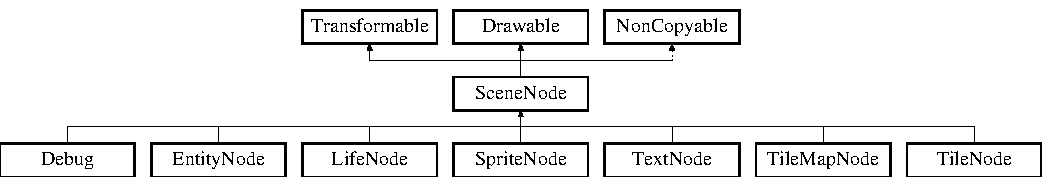
\includegraphics[height=2.376238cm]{classSceneNode}
\end{center}
\end{figure}
\subsection*{Tipos públicos}
\begin{DoxyCompactItemize}
\item 
\hypertarget{classSceneNode_a366efca54698fa3f6eaf80b41e7ff4df}{}typedef std\+::pair$<$ \hyperlink{classSceneNode}{Scene\+Node} $\ast$, \hyperlink{classSceneNode}{Scene\+Node} $\ast$ $>$ {\bfseries Pair}\label{classSceneNode_a366efca54698fa3f6eaf80b41e7ff4df}

\end{DoxyCompactItemize}
\subsection*{Métodos públicos}
\begin{DoxyCompactItemize}
\item 
\hyperlink{classSceneNode_acc2e7940323560ba86dad8e2d6eb6690}{Scene\+Node} ()
\item 
\hyperlink{classSceneNode_af87e82dcbe9fc195a557bc91a4b16317}{Scene\+Node} (Category category)
\item 
void \hyperlink{classSceneNode_a0e5790af868dcf846f37630094850fd7}{add\+Child} (\hyperlink{classSceneNode}{Scene\+Node} $\ast$child)
\item 
\hyperlink{classSceneNode}{Scene\+Node} $\ast$ \hyperlink{classSceneNode_a6fe848553acf7282b1faf6aaad3eb1b8}{remove\+Child} (const \hyperlink{classSceneNode}{Scene\+Node} \&node)
\item 
sf\+::\+Transform \hyperlink{classSceneNode_a88be3d3c93c80ee4a7ba25024d2414ec}{get\+World\+Transform} () const 
\item 
sf\+::\+Vector2f \hyperlink{classSceneNode_a410150636d06294c7a9e238d8c4f07b5}{get\+World\+Position} () const 
\item 
\hypertarget{classSceneNode_a132fa45a0a23ba86b76247273a16cfce}{}void {\bfseries update} (sf\+::\+Time dt)\label{classSceneNode_a132fa45a0a23ba86b76247273a16cfce}

\item 
\hypertarget{classSceneNode_a6c42640df0126ae10c4fa02d3bbfd509}{}virtual void {\bfseries update\+Second\+Part} (sf\+::\+Time dt)\label{classSceneNode_a6c42640df0126ae10c4fa02d3bbfd509}

\item 
virtual unsigned int \hyperlink{classSceneNode_a46b4d2304c0e3e8e18235959f51689d9}{get\+Category} () const 
\item 
void \hyperlink{classSceneNode_a4ab07dfa68f4094e2e9152b6f4869794}{remove\+Wrecks} ()
\item 
\hypertarget{classSceneNode_a7c07379dc7bd3165843607beb6287ef9}{}virtual bool {\bfseries is\+Marked\+For\+Removal} () const \label{classSceneNode_a7c07379dc7bd3165843607beb6287ef9}

\item 
virtual bool \hyperlink{classSceneNode_a2299b0d13e03f162adfd560bc29da734}{is\+Destroyed} () const 
\item 
float \hyperlink{classSceneNode_afb5602a1256e41b0375e8723368a05af}{get\+X\+Offset} () const 
\item 
float \hyperlink{classSceneNode_a8e8b4174abf121a96a2c950a9fbc001c}{get\+Y\+Offset} () const 
\item 
void \hyperlink{classSceneNode_a93362a6a508d77212c788bbf17814f96}{set\+X\+Offset} (float \hyperlink{classSceneNode_ad7b83da569e61908f0e828c11549610f}{x\+Offset})
\item 
void \hyperlink{classSceneNode_a0248f3ff0c2f90fd8464a87c13d90494}{set\+Y\+Offset} (float \hyperlink{classSceneNode_ac2e7bda67762d356a06386e271f41c23}{y\+Offset})
\end{DoxyCompactItemize}
\subsection*{Atributos protegidos}
\begin{DoxyCompactItemize}
\item 
float \hyperlink{classSceneNode_ad7b83da569e61908f0e828c11549610f}{x\+Offset}
\item 
float \hyperlink{classSceneNode_ac2e7bda67762d356a06386e271f41c23}{y\+Offset}
\item 
std\+::vector$<$ \hyperlink{classSceneNode}{Scene\+Node} $\ast$ $>$ \hyperlink{classSceneNode_a1dd91a11c15e87908157b3156da3d8cf}{children}
\end{DoxyCompactItemize}


\subsection{Descripción detallada}
Defines a node from a scene graph Can be drawed, has a position and orientation and can\textquotesingle{}t be cloned 

\subsection{Documentación del constructor y destructor}
\hypertarget{classSceneNode_acc2e7940323560ba86dad8e2d6eb6690}{}\index{Scene\+Node@{Scene\+Node}!Scene\+Node@{Scene\+Node}}
\index{Scene\+Node@{Scene\+Node}!Scene\+Node@{Scene\+Node}}
\subsubsection[{Scene\+Node}]{\setlength{\rightskip}{0pt plus 5cm}Scene\+Node\+::\+Scene\+Node (
\begin{DoxyParamCaption}
{}
\end{DoxyParamCaption}
)}\label{classSceneNode_acc2e7940323560ba86dad8e2d6eb6690}
Constructor \hypertarget{classSceneNode_af87e82dcbe9fc195a557bc91a4b16317}{}\index{Scene\+Node@{Scene\+Node}!Scene\+Node@{Scene\+Node}}
\index{Scene\+Node@{Scene\+Node}!Scene\+Node@{Scene\+Node}}
\subsubsection[{Scene\+Node}]{\setlength{\rightskip}{0pt plus 5cm}Scene\+Node\+::\+Scene\+Node (
\begin{DoxyParamCaption}
\item[{Category}]{category}
\end{DoxyParamCaption}
)}\label{classSceneNode_af87e82dcbe9fc195a557bc91a4b16317}
Constructor especificando la categoría 
\begin{DoxyParams}{Parámetros}
{\em category} & categoría del nodo \\
\hline
\end{DoxyParams}


\subsection{Documentación de las funciones miembro}
\hypertarget{classSceneNode_a0e5790af868dcf846f37630094850fd7}{}\index{Scene\+Node@{Scene\+Node}!add\+Child@{add\+Child}}
\index{add\+Child@{add\+Child}!Scene\+Node@{Scene\+Node}}
\subsubsection[{add\+Child}]{\setlength{\rightskip}{0pt plus 5cm}void Scene\+Node\+::add\+Child (
\begin{DoxyParamCaption}
\item[{{\bf Scene\+Node} $\ast$}]{child}
\end{DoxyParamCaption}
)}\label{classSceneNode_a0e5790af868dcf846f37630094850fd7}
Add a node to this node 
\begin{DoxyParams}{Parámetros}
{\em child} & the child \\
\hline
\end{DoxyParams}
\hypertarget{classSceneNode_a46b4d2304c0e3e8e18235959f51689d9}{}\index{Scene\+Node@{Scene\+Node}!get\+Category@{get\+Category}}
\index{get\+Category@{get\+Category}!Scene\+Node@{Scene\+Node}}
\subsubsection[{get\+Category}]{\setlength{\rightskip}{0pt plus 5cm}unsigned int Scene\+Node\+::get\+Category (
\begin{DoxyParamCaption}
{}
\end{DoxyParamCaption}
) const\hspace{0.3cm}{\ttfamily [virtual]}}\label{classSceneNode_a46b4d2304c0e3e8e18235959f51689d9}
Get the category of this node. \begin{DoxyReturn}{Devuelve}
the category of the node 
\end{DoxyReturn}
\hypertarget{classSceneNode_a410150636d06294c7a9e238d8c4f07b5}{}\index{Scene\+Node@{Scene\+Node}!get\+World\+Position@{get\+World\+Position}}
\index{get\+World\+Position@{get\+World\+Position}!Scene\+Node@{Scene\+Node}}
\subsubsection[{get\+World\+Position}]{\setlength{\rightskip}{0pt plus 5cm}sf\+::\+Vector2f Scene\+Node\+::get\+World\+Position (
\begin{DoxyParamCaption}
{}
\end{DoxyParamCaption}
) const}\label{classSceneNode_a410150636d06294c7a9e238d8c4f07b5}
Get the relative position of the node \begin{DoxyReturn}{Devuelve}
a vector x,y of floats 
\end{DoxyReturn}
\hypertarget{classSceneNode_a88be3d3c93c80ee4a7ba25024d2414ec}{}\index{Scene\+Node@{Scene\+Node}!get\+World\+Transform@{get\+World\+Transform}}
\index{get\+World\+Transform@{get\+World\+Transform}!Scene\+Node@{Scene\+Node}}
\subsubsection[{get\+World\+Transform}]{\setlength{\rightskip}{0pt plus 5cm}sf\+::\+Transform Scene\+Node\+::get\+World\+Transform (
\begin{DoxyParamCaption}
{}
\end{DoxyParamCaption}
) const}\label{classSceneNode_a88be3d3c93c80ee4a7ba25024d2414ec}
Get the absolute transform (position/rotation and scale) of the node \begin{DoxyReturn}{Devuelve}
the absolute transform 
\end{DoxyReturn}
\hypertarget{classSceneNode_afb5602a1256e41b0375e8723368a05af}{}\index{Scene\+Node@{Scene\+Node}!get\+X\+Offset@{get\+X\+Offset}}
\index{get\+X\+Offset@{get\+X\+Offset}!Scene\+Node@{Scene\+Node}}
\subsubsection[{get\+X\+Offset}]{\setlength{\rightskip}{0pt plus 5cm}float Scene\+Node\+::get\+X\+Offset (
\begin{DoxyParamCaption}
{}
\end{DoxyParamCaption}
) const\hspace{0.3cm}{\ttfamily [inline]}}\label{classSceneNode_afb5602a1256e41b0375e8723368a05af}
Devuelve el desplazamiento en el eje X, si lo hubiera, a efectos de ordenar y dar sensación de profundidad \begin{DoxyReturn}{Devuelve}
el offset en el eje x 
\end{DoxyReturn}
\hypertarget{classSceneNode_a8e8b4174abf121a96a2c950a9fbc001c}{}\index{Scene\+Node@{Scene\+Node}!get\+Y\+Offset@{get\+Y\+Offset}}
\index{get\+Y\+Offset@{get\+Y\+Offset}!Scene\+Node@{Scene\+Node}}
\subsubsection[{get\+Y\+Offset}]{\setlength{\rightskip}{0pt plus 5cm}float Scene\+Node\+::get\+Y\+Offset (
\begin{DoxyParamCaption}
{}
\end{DoxyParamCaption}
) const\hspace{0.3cm}{\ttfamily [inline]}}\label{classSceneNode_a8e8b4174abf121a96a2c950a9fbc001c}
Devuelve el desplazamiento en el eje Y, si lo hubiera, a efectos de ordenar y dar sensación de profundidad \begin{DoxyReturn}{Devuelve}
el offset en el eje y 
\end{DoxyReturn}
\hypertarget{classSceneNode_a2299b0d13e03f162adfd560bc29da734}{}\index{Scene\+Node@{Scene\+Node}!is\+Destroyed@{is\+Destroyed}}
\index{is\+Destroyed@{is\+Destroyed}!Scene\+Node@{Scene\+Node}}
\subsubsection[{is\+Destroyed}]{\setlength{\rightskip}{0pt plus 5cm}bool Scene\+Node\+::is\+Destroyed (
\begin{DoxyParamCaption}
{}
\end{DoxyParamCaption}
) const\hspace{0.3cm}{\ttfamily [virtual]}}\label{classSceneNode_a2299b0d13e03f162adfd560bc29da734}
Devuelve si el nodo está destruido \begin{DoxyReturn}{Devuelve}
true si esta destruido 
\end{DoxyReturn}
\hypertarget{classSceneNode_a6fe848553acf7282b1faf6aaad3eb1b8}{}\index{Scene\+Node@{Scene\+Node}!remove\+Child@{remove\+Child}}
\index{remove\+Child@{remove\+Child}!Scene\+Node@{Scene\+Node}}
\subsubsection[{remove\+Child}]{\setlength{\rightskip}{0pt plus 5cm}{\bf Scene\+Node} $\ast$ Scene\+Node\+::remove\+Child (
\begin{DoxyParamCaption}
\item[{const {\bf Scene\+Node} \&}]{node}
\end{DoxyParamCaption}
)}\label{classSceneNode_a6fe848553acf7282b1faf6aaad3eb1b8}
Remove the given node to this node 
\begin{DoxyParams}{Parámetros}
{\em node} & the child to remove \\
\hline
\end{DoxyParams}
\begin{DoxyReturn}{Devuelve}
the removed node 
\end{DoxyReturn}
\hypertarget{classSceneNode_a4ab07dfa68f4094e2e9152b6f4869794}{}\index{Scene\+Node@{Scene\+Node}!remove\+Wrecks@{remove\+Wrecks}}
\index{remove\+Wrecks@{remove\+Wrecks}!Scene\+Node@{Scene\+Node}}
\subsubsection[{remove\+Wrecks}]{\setlength{\rightskip}{0pt plus 5cm}void Scene\+Node\+::remove\+Wrecks (
\begin{DoxyParamCaption}
{}
\end{DoxyParamCaption}
)}\label{classSceneNode_a4ab07dfa68f4094e2e9152b6f4869794}
Elimina los nodos marcados \hypertarget{classSceneNode_a93362a6a508d77212c788bbf17814f96}{}\index{Scene\+Node@{Scene\+Node}!set\+X\+Offset@{set\+X\+Offset}}
\index{set\+X\+Offset@{set\+X\+Offset}!Scene\+Node@{Scene\+Node}}
\subsubsection[{set\+X\+Offset}]{\setlength{\rightskip}{0pt plus 5cm}void Scene\+Node\+::set\+X\+Offset (
\begin{DoxyParamCaption}
\item[{float}]{x\+Offset}
\end{DoxyParamCaption}
)\hspace{0.3cm}{\ttfamily [inline]}}\label{classSceneNode_a93362a6a508d77212c788bbf17814f96}
Setea el offset en el eje x 
\begin{DoxyParams}{Parámetros}
{\em x\+Offset} & offset en el eje x \\
\hline
\end{DoxyParams}
\hypertarget{classSceneNode_a0248f3ff0c2f90fd8464a87c13d90494}{}\index{Scene\+Node@{Scene\+Node}!set\+Y\+Offset@{set\+Y\+Offset}}
\index{set\+Y\+Offset@{set\+Y\+Offset}!Scene\+Node@{Scene\+Node}}
\subsubsection[{set\+Y\+Offset}]{\setlength{\rightskip}{0pt plus 5cm}void Scene\+Node\+::set\+Y\+Offset (
\begin{DoxyParamCaption}
\item[{float}]{y\+Offset}
\end{DoxyParamCaption}
)\hspace{0.3cm}{\ttfamily [inline]}}\label{classSceneNode_a0248f3ff0c2f90fd8464a87c13d90494}
Setea el offset en el eje y 
\begin{DoxyParams}{Parámetros}
{\em x\+Offset} & offset en el eje y \\
\hline
\end{DoxyParams}


\subsection{Documentación de los campos}
\hypertarget{classSceneNode_a1dd91a11c15e87908157b3156da3d8cf}{}\index{Scene\+Node@{Scene\+Node}!children@{children}}
\index{children@{children}!Scene\+Node@{Scene\+Node}}
\subsubsection[{children}]{\setlength{\rightskip}{0pt plus 5cm}std\+::vector$<${\bf Scene\+Node}$\ast$$>$ Scene\+Node\+::children\hspace{0.3cm}{\ttfamily [protected]}}\label{classSceneNode_a1dd91a11c15e87908157b3156da3d8cf}
\hyperlink{classVector}{Vector} of children nodes \hypertarget{classSceneNode_ad7b83da569e61908f0e828c11549610f}{}\index{Scene\+Node@{Scene\+Node}!x\+Offset@{x\+Offset}}
\index{x\+Offset@{x\+Offset}!Scene\+Node@{Scene\+Node}}
\subsubsection[{x\+Offset}]{\setlength{\rightskip}{0pt plus 5cm}float Scene\+Node\+::x\+Offset\hspace{0.3cm}{\ttfamily [protected]}}\label{classSceneNode_ad7b83da569e61908f0e828c11549610f}
Desplazamiento en el eje x \hypertarget{classSceneNode_ac2e7bda67762d356a06386e271f41c23}{}\index{Scene\+Node@{Scene\+Node}!y\+Offset@{y\+Offset}}
\index{y\+Offset@{y\+Offset}!Scene\+Node@{Scene\+Node}}
\subsubsection[{y\+Offset}]{\setlength{\rightskip}{0pt plus 5cm}float Scene\+Node\+::y\+Offset\hspace{0.3cm}{\ttfamily [protected]}}\label{classSceneNode_ac2e7bda67762d356a06386e271f41c23}
Desplazamiento en el eje y 

La documentación para esta clase fue generada a partir de los siguientes ficheros\+:\begin{DoxyCompactItemize}
\item 
Scene\+Node.\+h\item 
Scene\+Node.\+cpp\end{DoxyCompactItemize}

\hypertarget{classSettingsState}{}\section{Referencia de la Clase Settings\+State}
\label{classSettingsState}\index{Settings\+State@{Settings\+State}}


{\ttfamily \#include $<$Settings\+State.\+h$>$}

Diagrama de herencias de Settings\+State\begin{figure}[H]
\begin{center}
\leavevmode
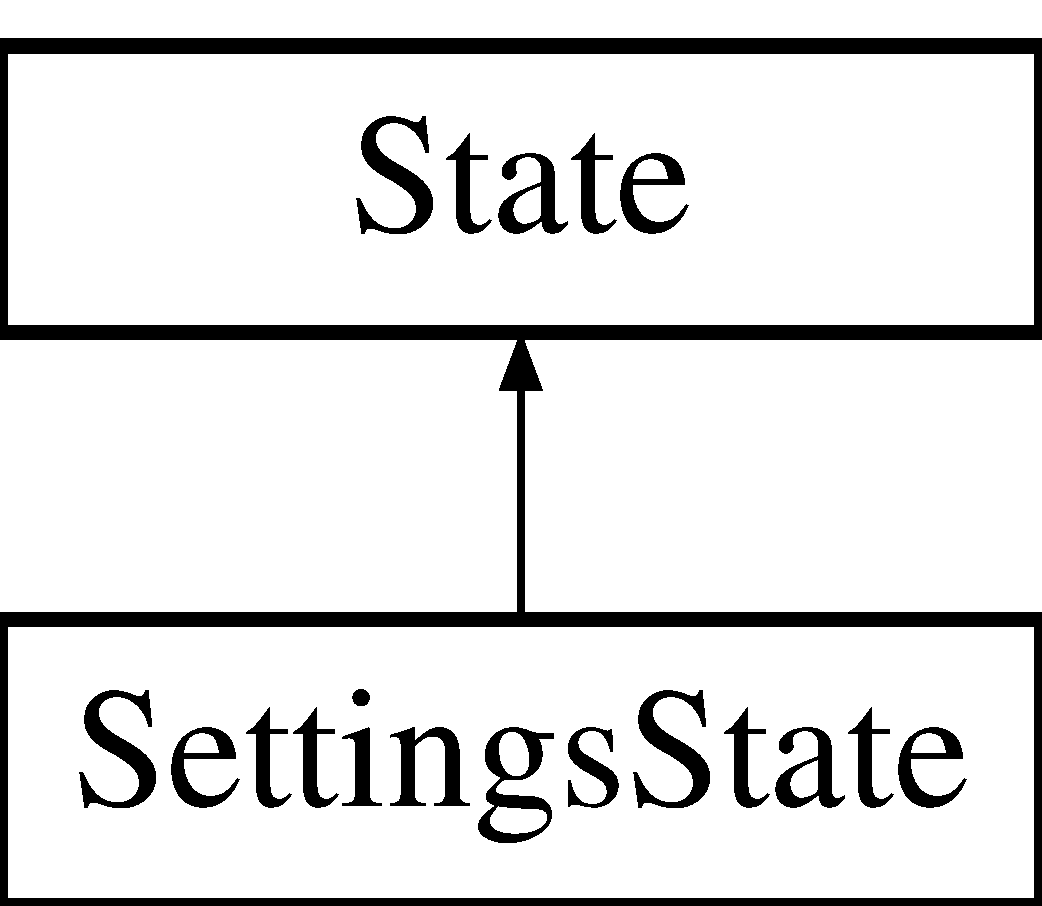
\includegraphics[height=2.000000cm]{classSettingsState}
\end{center}
\end{figure}
\subsection*{Métodos públicos}
\begin{DoxyCompactItemize}
\item 
\hyperlink{classSettingsState_a67ad7173de1a0fa00d8746fc88fdb2b5}{Settings\+State} (\hyperlink{classStateStack}{State\+Stack} \&\hyperlink{classState_a86c8d3a5a1ee89896828be85a785fb04}{stack}, \hyperlink{classContext}{Context} $\ast$\hyperlink{classState_adc93e8ad3199b5891618ca88eed0436a}{context})
\item 
virtual void \hyperlink{classSettingsState_afb948fe782ad303939a3833030898d5c}{draw} ()
\item 
virtual bool \hyperlink{classSettingsState_a8b93195e2c3d037cbf4b61add04081c2}{update} (sf\+::\+Time dt)
\item 
virtual bool \hyperlink{classSettingsState_a21fddce7003c26dd485154df18261be5}{handle\+Event} (const sf\+::\+Event \&event)
\item 
virtual void \hyperlink{classSettingsState_a0815b26acaac5860b227c9d641842c88}{pushed\+Action} ()
\end{DoxyCompactItemize}
\subsection*{Otros miembros heredados}


\subsection{Descripción detallada}
Representa la pantalla de opciones. Permite cambiar el mapeo del teclado 

\subsection{Documentación del constructor y destructor}
\hypertarget{classSettingsState_a67ad7173de1a0fa00d8746fc88fdb2b5}{}\index{Settings\+State@{Settings\+State}!Settings\+State@{Settings\+State}}
\index{Settings\+State@{Settings\+State}!Settings\+State@{Settings\+State}}
\subsubsection[{Settings\+State}]{\setlength{\rightskip}{0pt plus 5cm}Settings\+State\+::\+Settings\+State (
\begin{DoxyParamCaption}
\item[{{\bf State\+Stack} \&}]{stack, }
\item[{{\bf Context} $\ast$}]{context}
\end{DoxyParamCaption}
)}\label{classSettingsState_a67ad7173de1a0fa00d8746fc88fdb2b5}
Constructor 
\begin{DoxyParams}{Parámetros}
{\em stack} & \\
\hline
{\em context} & \\
\hline
\end{DoxyParams}


\subsection{Documentación de las funciones miembro}
\hypertarget{classSettingsState_afb948fe782ad303939a3833030898d5c}{}\index{Settings\+State@{Settings\+State}!draw@{draw}}
\index{draw@{draw}!Settings\+State@{Settings\+State}}
\subsubsection[{draw}]{\setlength{\rightskip}{0pt plus 5cm}void Settings\+State\+::draw (
\begin{DoxyParamCaption}
{}
\end{DoxyParamCaption}
)\hspace{0.3cm}{\ttfamily [virtual]}}\label{classSettingsState_afb948fe782ad303939a3833030898d5c}
Dibuja el estado 

Implementa \hyperlink{classState_ae261605bc40b7e3959ce5df5457e4942}{State}.

\hypertarget{classSettingsState_a21fddce7003c26dd485154df18261be5}{}\index{Settings\+State@{Settings\+State}!handle\+Event@{handle\+Event}}
\index{handle\+Event@{handle\+Event}!Settings\+State@{Settings\+State}}
\subsubsection[{handle\+Event}]{\setlength{\rightskip}{0pt plus 5cm}bool Settings\+State\+::handle\+Event (
\begin{DoxyParamCaption}
\item[{const sf\+::\+Event \&}]{event}
\end{DoxyParamCaption}
)\hspace{0.3cm}{\ttfamily [virtual]}}\label{classSettingsState_a21fddce7003c26dd485154df18261be5}
Procesa la entrada del usuario 
\begin{DoxyParams}{Parámetros}
{\em event} & evento \\
\hline
\end{DoxyParams}
\begin{DoxyReturn}{Devuelve}
true si lo ha procesado, false si no (o lo ha procesado pero que continúe) 
\end{DoxyReturn}


Implementa \hyperlink{classState_a19965f83460b248c42952aac8d001206}{State}.

\hypertarget{classSettingsState_a0815b26acaac5860b227c9d641842c88}{}\index{Settings\+State@{Settings\+State}!pushed\+Action@{pushed\+Action}}
\index{pushed\+Action@{pushed\+Action}!Settings\+State@{Settings\+State}}
\subsubsection[{pushed\+Action}]{\setlength{\rightskip}{0pt plus 5cm}void Settings\+State\+::pushed\+Action (
\begin{DoxyParamCaption}
{}
\end{DoxyParamCaption}
)\hspace{0.3cm}{\ttfamily [virtual]}}\label{classSettingsState_a0815b26acaac5860b227c9d641842c88}
Método ejecutado cuando es puesto en pila 

Reimplementado de \hyperlink{classState_a3cc6a1378f32f9ed6a2d1d8140296808}{State}.

\hypertarget{classSettingsState_a8b93195e2c3d037cbf4b61add04081c2}{}\index{Settings\+State@{Settings\+State}!update@{update}}
\index{update@{update}!Settings\+State@{Settings\+State}}
\subsubsection[{update}]{\setlength{\rightskip}{0pt plus 5cm}bool Settings\+State\+::update (
\begin{DoxyParamCaption}
\item[{sf\+::\+Time}]{delta}
\end{DoxyParamCaption}
)\hspace{0.3cm}{\ttfamily [virtual]}}\label{classSettingsState_a8b93195e2c3d037cbf4b61add04081c2}
Actualiza el estado 
\begin{DoxyParams}{Parámetros}
{\em delta} & tiempo entre frame y frame \\
\hline
\end{DoxyParams}
\begin{DoxyReturn}{Devuelve}
true si se ha actualizado 
\end{DoxyReturn}


Implementa \hyperlink{classState_aa6366828eb50639e86b94008cfad9c5d}{State}.



La documentación para esta clase fue generada a partir de los siguientes ficheros\+:\begin{DoxyCompactItemize}
\item 
Settings\+State.\+h\item 
Settings\+State.\+cpp\end{DoxyCompactItemize}

\hypertarget{classSoundPlayer}{}\section{Referencia de la Clase Sound\+Player}
\label{classSoundPlayer}\index{Sound\+Player@{Sound\+Player}}
Diagrama de herencias de Sound\+Player\begin{figure}[H]
\begin{center}
\leavevmode
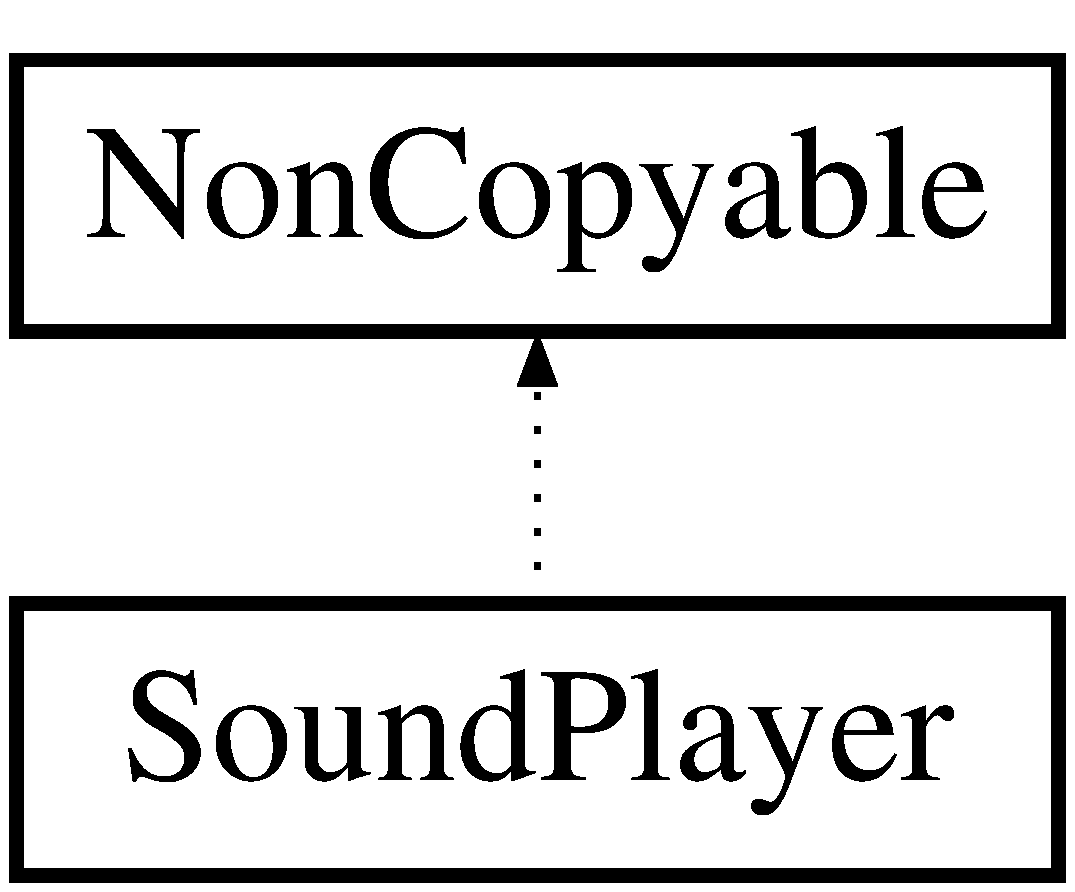
\includegraphics[height=2.000000cm]{classSoundPlayer}
\end{center}
\end{figure}
\subsection*{Métodos públicos}
\begin{DoxyCompactItemize}
\item 
\hypertarget{classSoundPlayer_a016133f69b26dc403af68760a4ca9ed3}{}void {\bfseries play} (Sound\+Effect\+I\+D effect)\label{classSoundPlayer_a016133f69b26dc403af68760a4ca9ed3}

\item 
\hypertarget{classSoundPlayer_aa596ffd50028d9614f14fcd55c22dbc2}{}void {\bfseries play} (Sound\+Effect\+I\+D effect, sf\+::\+Vector2f position)\label{classSoundPlayer_aa596ffd50028d9614f14fcd55c22dbc2}

\item 
\hypertarget{classSoundPlayer_a3fd165dadf60b580b16367b81d84681b}{}void {\bfseries remove\+Stopped\+Sounds} ()\label{classSoundPlayer_a3fd165dadf60b580b16367b81d84681b}

\item 
\hypertarget{classSoundPlayer_abfd270417c9490f1c0f92b0c4986fa52}{}void {\bfseries set\+Listener\+Position} (sf\+::\+Vector2f position)\label{classSoundPlayer_abfd270417c9490f1c0f92b0c4986fa52}

\item 
\hypertarget{classSoundPlayer_ae0ec5bc31ee027fab6e71984ff13388d}{}sf\+::\+Vector2f {\bfseries get\+Listener\+Position} () const \label{classSoundPlayer_ae0ec5bc31ee027fab6e71984ff13388d}

\end{DoxyCompactItemize}


La documentación para esta clase fue generada a partir de los siguientes ficheros\+:\begin{DoxyCompactItemize}
\item 
Sound\+Player.\+h\item 
Sound\+Player.\+cpp\end{DoxyCompactItemize}

\hypertarget{classSpriteNode}{}\section{Referencia de la Clase Sprite\+Node}
\label{classSpriteNode}\index{Sprite\+Node@{Sprite\+Node}}


{\ttfamily \#include $<$Sprite\+Node.\+h$>$}

Diagrama de herencias de Sprite\+Node\begin{figure}[H]
\begin{center}
\leavevmode
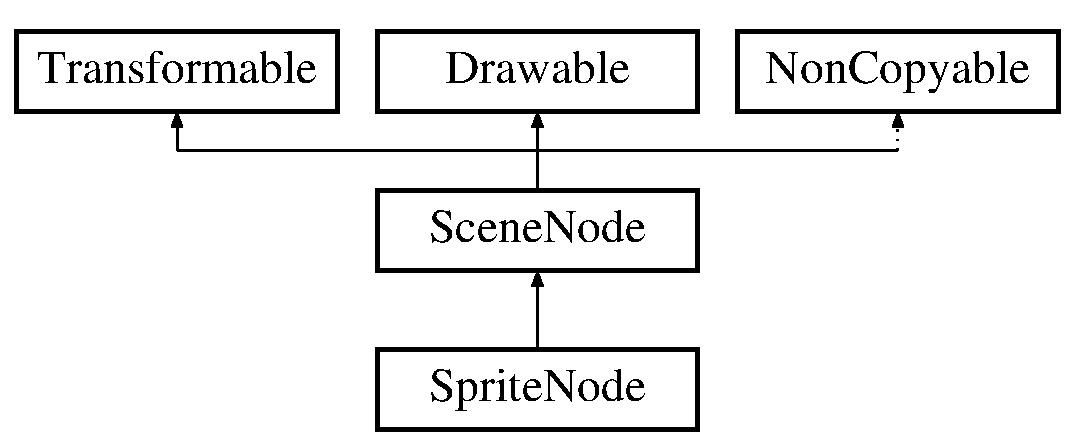
\includegraphics[height=3.000000cm]{classSpriteNode}
\end{center}
\end{figure}
\subsection*{Métodos públicos}
\begin{DoxyCompactItemize}
\item 
\hyperlink{classSpriteNode_ad72b769f4c57e5d77a8d6ba223f487b0}{Sprite\+Node} (const sf\+::\+Texture \&texture)
\item 
\hyperlink{classSpriteNode_ac12927969dcfd6f02da372e7e22c2af1}{Sprite\+Node} (const sf\+::\+Texture \&texture, const sf\+::\+Int\+Rect \&texture\+Rect)
\item 
virtual void \hyperlink{classSpriteNode_a30748234dea11083eafb7b22f9567e52}{draw\+Current} (sf\+::\+Render\+Target \&target, sf\+::\+Render\+States states) const 
\end{DoxyCompactItemize}
\subsection*{Otros miembros heredados}


\subsection{Descripción detallada}
A concrete \hyperlink{classSceneNode}{Scene\+Node} with a sprite to draw 

\subsection{Documentación del constructor y destructor}
\hypertarget{classSpriteNode_ad72b769f4c57e5d77a8d6ba223f487b0}{}\index{Sprite\+Node@{Sprite\+Node}!Sprite\+Node@{Sprite\+Node}}
\index{Sprite\+Node@{Sprite\+Node}!Sprite\+Node@{Sprite\+Node}}
\subsubsection[{Sprite\+Node}]{\setlength{\rightskip}{0pt plus 5cm}Sprite\+Node\+::\+Sprite\+Node (
\begin{DoxyParamCaption}
\item[{const sf\+::\+Texture \&}]{texture}
\end{DoxyParamCaption}
)}\label{classSpriteNode_ad72b769f4c57e5d77a8d6ba223f487b0}
Constructor 
\begin{DoxyParams}{Parámetros}
{\em texture} & of the sprite \\
\hline
\end{DoxyParams}
\hypertarget{classSpriteNode_ac12927969dcfd6f02da372e7e22c2af1}{}\index{Sprite\+Node@{Sprite\+Node}!Sprite\+Node@{Sprite\+Node}}
\index{Sprite\+Node@{Sprite\+Node}!Sprite\+Node@{Sprite\+Node}}
\subsubsection[{Sprite\+Node}]{\setlength{\rightskip}{0pt plus 5cm}Sprite\+Node\+::\+Sprite\+Node (
\begin{DoxyParamCaption}
\item[{const sf\+::\+Texture \&}]{texture, }
\item[{const sf\+::\+Int\+Rect \&}]{texture\+Rect}
\end{DoxyParamCaption}
)}\label{classSpriteNode_ac12927969dcfd6f02da372e7e22c2af1}
Constructor para cuando no es la imagen entera, sino una zona concreta 
\begin{DoxyParams}{Parámetros}
{\em texture} & of the sprite \\
\hline
{\em texture\+Rect} & region of the texture to draw \\
\hline
\end{DoxyParams}


\subsection{Documentación de las funciones miembro}
\hypertarget{classSpriteNode_a30748234dea11083eafb7b22f9567e52}{}\index{Sprite\+Node@{Sprite\+Node}!draw\+Current@{draw\+Current}}
\index{draw\+Current@{draw\+Current}!Sprite\+Node@{Sprite\+Node}}
\subsubsection[{draw\+Current}]{\setlength{\rightskip}{0pt plus 5cm}void Sprite\+Node\+::draw\+Current (
\begin{DoxyParamCaption}
\item[{sf\+::\+Render\+Target \&}]{target, }
\item[{sf\+::\+Render\+States}]{states}
\end{DoxyParamCaption}
) const\hspace{0.3cm}{\ttfamily [virtual]}}\label{classSpriteNode_a30748234dea11083eafb7b22f9567e52}
Inherit from \hyperlink{classSceneNode}{Scene\+Node}, draw the sprite 
\begin{DoxyParams}{Parámetros}
{\em target} & \\
\hline
{\em states} & \\
\hline
\end{DoxyParams}


Reimplementado de \hyperlink{classSceneNode}{Scene\+Node}.



La documentación para esta clase fue generada a partir de los siguientes ficheros\+:\begin{DoxyCompactItemize}
\item 
Sprite\+Node.\+h\item 
Sprite\+Node.\+cpp\end{DoxyCompactItemize}

\hypertarget{classState}{}\section{Referencia de la Clase State}
\label{classState}\index{State@{State}}


{\ttfamily \#include $<$State.\+h$>$}

Diagrama de herencias de State\begin{figure}[H]
\begin{center}
\leavevmode
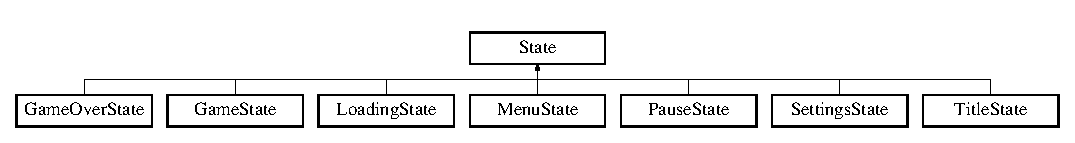
\includegraphics[height=1.467890cm]{classState}
\end{center}
\end{figure}
\subsection*{Métodos públicos}
\begin{DoxyCompactItemize}
\item 
\hyperlink{classState_ae4dcb70a7ad6a1bfe13fcda87600806d}{State} (\hyperlink{classStateStack}{State\+Stack} \&\hyperlink{classState_a86c8d3a5a1ee89896828be85a785fb04}{stack}, \hyperlink{classContext}{Context} $\ast$\hyperlink{classState_adc93e8ad3199b5891618ca88eed0436a}{context})
\item 
virtual \hyperlink{classState_afab438d92b90dc18d194dbd9c9c8bab3}{$\sim$\+State} ()
\item 
virtual void \hyperlink{classState_ae261605bc40b7e3959ce5df5457e4942}{draw} ()=0
\item 
virtual bool \hyperlink{classState_aa6366828eb50639e86b94008cfad9c5d}{update} (sf\+::\+Time delta)=0
\item 
virtual bool \hyperlink{classState_a19965f83460b248c42952aac8d001206}{handle\+Event} (const sf\+::\+Event \&event)=0
\item 
virtual void \hyperlink{classState_a3cc6a1378f32f9ed6a2d1d8140296808}{pushed\+Action} ()
\item 
virtual void \hyperlink{classState_a92620c4648de675037b20ec59edb52a3}{pulled\+Action} ()
\end{DoxyCompactItemize}
\subsection*{Métodos protegidos}
\begin{DoxyCompactItemize}
\item 
void \hyperlink{classState_a0560458d8f71d6fc0e239e726552ea26}{request\+Stack\+Push} (States\+I\+D state)
\item 
void \hyperlink{classState_aa418660892d6161772c907bd8d70f910}{request\+Stack\+Pop} ()
\item 
void \hyperlink{classState_a4b602bed9bf0179ee5f6748fce340ae6}{request\+State\+Clear} ()
\item 
\hyperlink{classContext}{Context} $\ast$ \hyperlink{classState_ab08e1a541e46b2335c92ecbafe369df5}{get\+Context} () const 
\end{DoxyCompactItemize}
\subsection*{Atributos protegidos}
\begin{DoxyCompactItemize}
\item 
\hyperlink{classStateStack}{State\+Stack} $\ast$ \hyperlink{classState_a86c8d3a5a1ee89896828be85a785fb04}{stack}
\item 
\hyperlink{classContext}{Context} $\ast$ \hyperlink{classState_adc93e8ad3199b5891618ca88eed0436a}{context}
\end{DoxyCompactItemize}


\subsection{Descripción detallada}
Clase base de estados 

\subsection{Documentación del constructor y destructor}
\hypertarget{classState_ae4dcb70a7ad6a1bfe13fcda87600806d}{}\index{State@{State}!State@{State}}
\index{State@{State}!State@{State}}
\subsubsection[{State}]{\setlength{\rightskip}{0pt plus 5cm}State\+::\+State (
\begin{DoxyParamCaption}
\item[{{\bf State\+Stack} \&}]{stack, }
\item[{{\bf Context} $\ast$}]{context}
\end{DoxyParamCaption}
)}\label{classState_ae4dcb70a7ad6a1bfe13fcda87600806d}
Constructor 
\begin{DoxyParams}{Parámetros}
{\em stack} & pila de estados \\
\hline
{\em context} & contexto \\
\hline
\end{DoxyParams}
\hypertarget{classState_afab438d92b90dc18d194dbd9c9c8bab3}{}\index{State@{State}!````~State@{$\sim$\+State}}
\index{````~State@{$\sim$\+State}!State@{State}}
\subsubsection[{$\sim$\+State}]{\setlength{\rightskip}{0pt plus 5cm}State\+::$\sim$\+State (
\begin{DoxyParamCaption}
{}
\end{DoxyParamCaption}
)\hspace{0.3cm}{\ttfamily [virtual]}}\label{classState_afab438d92b90dc18d194dbd9c9c8bab3}
Destructor 

\subsection{Documentación de las funciones miembro}
\hypertarget{classState_ae261605bc40b7e3959ce5df5457e4942}{}\index{State@{State}!draw@{draw}}
\index{draw@{draw}!State@{State}}
\subsubsection[{draw}]{\setlength{\rightskip}{0pt plus 5cm}virtual void State\+::draw (
\begin{DoxyParamCaption}
{}
\end{DoxyParamCaption}
)\hspace{0.3cm}{\ttfamily [pure virtual]}}\label{classState_ae261605bc40b7e3959ce5df5457e4942}
Dibuja el estado 

Implementado en \hyperlink{classSettingsState_afb948fe782ad303939a3833030898d5c}{Settings\+State}, \hyperlink{classTitleState_ae12beafe5aad6929a56089942de1220e}{Title\+State}, \hyperlink{classPauseState_ac4c159c2f6d32eedd351f39e36c43f9d}{Pause\+State}, \hyperlink{classMenuState_aa557d6c3bf06bb3107ed780913a6b47f}{Menu\+State}, \hyperlink{classLoadingState_adfe2c002c52cc2c49967ba3ace4aa73b}{Loading\+State}, \hyperlink{classGameOverState_a9decc1411647e390bfed0bdc009cd691}{Game\+Over\+State} y \hyperlink{classGameState_a3c511417d8934943ae65c04681f321a3}{Game\+State}.

\hypertarget{classState_ab08e1a541e46b2335c92ecbafe369df5}{}\index{State@{State}!get\+Context@{get\+Context}}
\index{get\+Context@{get\+Context}!State@{State}}
\subsubsection[{get\+Context}]{\setlength{\rightskip}{0pt plus 5cm}{\bf Context} $\ast$ State\+::get\+Context (
\begin{DoxyParamCaption}
{}
\end{DoxyParamCaption}
) const\hspace{0.3cm}{\ttfamily [protected]}}\label{classState_ab08e1a541e46b2335c92ecbafe369df5}
Devuelve el contexto guardado en el estado \begin{DoxyReturn}{Devuelve}
contexto 
\end{DoxyReturn}
\hypertarget{classState_a19965f83460b248c42952aac8d001206}{}\index{State@{State}!handle\+Event@{handle\+Event}}
\index{handle\+Event@{handle\+Event}!State@{State}}
\subsubsection[{handle\+Event}]{\setlength{\rightskip}{0pt plus 5cm}virtual bool State\+::handle\+Event (
\begin{DoxyParamCaption}
\item[{const sf\+::\+Event \&}]{event}
\end{DoxyParamCaption}
)\hspace{0.3cm}{\ttfamily [pure virtual]}}\label{classState_a19965f83460b248c42952aac8d001206}
Procesa la entrada del usuario 
\begin{DoxyParams}{Parámetros}
{\em event} & evento \\
\hline
\end{DoxyParams}
\begin{DoxyReturn}{Devuelve}
true si lo ha procesado, false si no (o lo ha procesado pero que continúe) 
\end{DoxyReturn}


Implementado en \hyperlink{classSettingsState_a21fddce7003c26dd485154df18261be5}{Settings\+State}, \hyperlink{classTitleState_a91c6ab4d741fe7445d88ed603001971a}{Title\+State}, \hyperlink{classPauseState_a685dda66dca3e1c41f4cb02da93c5a8d}{Pause\+State}, \hyperlink{classMenuState_a04a21241cebf6a8f0fe8ee9ce895ef18}{Menu\+State}, \hyperlink{classLoadingState_a37da243eeeca36460bac2f32cef3e368}{Loading\+State}, \hyperlink{classGameOverState_acf1dc2c7f58fe21b7cfababaf87ff20b}{Game\+Over\+State} y \hyperlink{classGameState_a000dd3306b1cb9faab5a86774a22aa6d}{Game\+State}.

\hypertarget{classState_a92620c4648de675037b20ec59edb52a3}{}\index{State@{State}!pulled\+Action@{pulled\+Action}}
\index{pulled\+Action@{pulled\+Action}!State@{State}}
\subsubsection[{pulled\+Action}]{\setlength{\rightskip}{0pt plus 5cm}virtual void State\+::pulled\+Action (
\begin{DoxyParamCaption}
{}
\end{DoxyParamCaption}
)\hspace{0.3cm}{\ttfamily [inline]}, {\ttfamily [virtual]}}\label{classState_a92620c4648de675037b20ec59edb52a3}
Método ejecutado cuando es sacado de la pila 

Reimplementado en \hyperlink{classTitleState_ab27a65d03920cbbb9cff7f14cd23372c}{Title\+State}, \hyperlink{classPauseState_ac04578f84a4c4fbcdf2d8b963b5f9fd0}{Pause\+State} y \hyperlink{classMenuState_aa465ec731c1ab2b63a54ce5c59092ea3}{Menu\+State}.

\hypertarget{classState_a3cc6a1378f32f9ed6a2d1d8140296808}{}\index{State@{State}!pushed\+Action@{pushed\+Action}}
\index{pushed\+Action@{pushed\+Action}!State@{State}}
\subsubsection[{pushed\+Action}]{\setlength{\rightskip}{0pt plus 5cm}virtual void State\+::pushed\+Action (
\begin{DoxyParamCaption}
{}
\end{DoxyParamCaption}
)\hspace{0.3cm}{\ttfamily [inline]}, {\ttfamily [virtual]}}\label{classState_a3cc6a1378f32f9ed6a2d1d8140296808}
Método ejecutado cuando es puesto en pila 

Reimplementado en \hyperlink{classSettingsState_a0815b26acaac5860b227c9d641842c88}{Settings\+State}, \hyperlink{classTitleState_a6c10b4a33cf09388f0bcca1af0872f68}{Title\+State}, \hyperlink{classMenuState_a74beed2b1d43948dd7ab1b8262519df6}{Menu\+State}, \hyperlink{classPauseState_aa20ec5df0044a9652df788b9ad1aafb9}{Pause\+State}, \hyperlink{classGameOverState_aa0e79a90d666351a0328b051dece3024}{Game\+Over\+State} y \hyperlink{classGameState_aaff561d6fe2a21a2084d093016a1d3be}{Game\+State}.

\hypertarget{classState_aa418660892d6161772c907bd8d70f910}{}\index{State@{State}!request\+Stack\+Pop@{request\+Stack\+Pop}}
\index{request\+Stack\+Pop@{request\+Stack\+Pop}!State@{State}}
\subsubsection[{request\+Stack\+Pop}]{\setlength{\rightskip}{0pt plus 5cm}void State\+::request\+Stack\+Pop (
\begin{DoxyParamCaption}
{}
\end{DoxyParamCaption}
)\hspace{0.3cm}{\ttfamily [protected]}}\label{classState_aa418660892d6161772c907bd8d70f910}
P\+Ide sacar el último estado de la pila \hypertarget{classState_a0560458d8f71d6fc0e239e726552ea26}{}\index{State@{State}!request\+Stack\+Push@{request\+Stack\+Push}}
\index{request\+Stack\+Push@{request\+Stack\+Push}!State@{State}}
\subsubsection[{request\+Stack\+Push}]{\setlength{\rightskip}{0pt plus 5cm}void State\+::request\+Stack\+Push (
\begin{DoxyParamCaption}
\item[{States\+I\+D}]{state}
\end{DoxyParamCaption}
)\hspace{0.3cm}{\ttfamily [protected]}}\label{classState_a0560458d8f71d6fc0e239e726552ea26}
Pide poner un estado en pila 
\begin{DoxyParams}{Parámetros}
{\em state} & identificador del estado \\
\hline
\end{DoxyParams}
\hypertarget{classState_a4b602bed9bf0179ee5f6748fce340ae6}{}\index{State@{State}!request\+State\+Clear@{request\+State\+Clear}}
\index{request\+State\+Clear@{request\+State\+Clear}!State@{State}}
\subsubsection[{request\+State\+Clear}]{\setlength{\rightskip}{0pt plus 5cm}void State\+::request\+State\+Clear (
\begin{DoxyParamCaption}
{}
\end{DoxyParamCaption}
)\hspace{0.3cm}{\ttfamily [protected]}}\label{classState_a4b602bed9bf0179ee5f6748fce340ae6}
Pide limpiar la pila \hypertarget{classState_aa6366828eb50639e86b94008cfad9c5d}{}\index{State@{State}!update@{update}}
\index{update@{update}!State@{State}}
\subsubsection[{update}]{\setlength{\rightskip}{0pt plus 5cm}virtual bool State\+::update (
\begin{DoxyParamCaption}
\item[{sf\+::\+Time}]{delta}
\end{DoxyParamCaption}
)\hspace{0.3cm}{\ttfamily [pure virtual]}}\label{classState_aa6366828eb50639e86b94008cfad9c5d}
Actualiza el estado 
\begin{DoxyParams}{Parámetros}
{\em delta} & tiempo entre frame y frame \\
\hline
\end{DoxyParams}
\begin{DoxyReturn}{Devuelve}
true si se ha actualizado 
\end{DoxyReturn}


Implementado en \hyperlink{classSettingsState_a8b93195e2c3d037cbf4b61add04081c2}{Settings\+State}, \hyperlink{classTitleState_aa282ac0c6e22267cb6a7054973d75fdf}{Title\+State}, \hyperlink{classPauseState_aed5aa4149e29b9124ade7a76a63941cd}{Pause\+State}, \hyperlink{classMenuState_a24362f4096e0f76e02a7d1b26ac657af}{Menu\+State}, \hyperlink{classLoadingState_a8f1729b9b5ca91c0ec3918b86bfe8feb}{Loading\+State}, \hyperlink{classGameOverState_a8a2047b5c684965f33574b8aee7b7c8f}{Game\+Over\+State} y \hyperlink{classGameState_a4ac988f0da5c33b43ff356890fcf9c1c}{Game\+State}.



\subsection{Documentación de los campos}
\hypertarget{classState_adc93e8ad3199b5891618ca88eed0436a}{}\index{State@{State}!context@{context}}
\index{context@{context}!State@{State}}
\subsubsection[{context}]{\setlength{\rightskip}{0pt plus 5cm}{\bf Context}$\ast$ State\+::context\hspace{0.3cm}{\ttfamily [protected]}}\label{classState_adc93e8ad3199b5891618ca88eed0436a}
Contexto de la aplicación \hypertarget{classState_a86c8d3a5a1ee89896828be85a785fb04}{}\index{State@{State}!stack@{stack}}
\index{stack@{stack}!State@{State}}
\subsubsection[{stack}]{\setlength{\rightskip}{0pt plus 5cm}{\bf State\+Stack}$\ast$ State\+::stack\hspace{0.3cm}{\ttfamily [protected]}}\label{classState_a86c8d3a5a1ee89896828be85a785fb04}
P\+Ila de estados 

La documentación para esta clase fue generada a partir de los siguientes ficheros\+:\begin{DoxyCompactItemize}
\item 
State.\+h\item 
State.\+cpp\end{DoxyCompactItemize}

\hypertarget{classStateMachine}{}\section{Referencia de la Clase State\+Machine}
\label{classStateMachine}\index{State\+Machine@{State\+Machine}}


{\ttfamily \#include $<$State\+Machine.\+h$>$}

\subsection*{Métodos públicos}
\begin{DoxyCompactItemize}
\item 
\hyperlink{classStateMachine_abff0cdd38e44a9af31972fd01d599348}{State\+Machine} (int number\+States)
\item 
void \hyperlink{classStateMachine_abc849e79ebc1b9d5fdcdef05ee76c6fc}{add\+Transition} (\hyperlink{structTransition}{Transition} \&transition)
\item 
int \hyperlink{classStateMachine_ae386ede5033e27c114e88bdd830a6ff2}{get\+State} ()
\item 
int \hyperlink{classStateMachine_a88789321a07bc082031f87a6a43d9ad7}{process\+Entry} (int entry)
\end{DoxyCompactItemize}


\subsection{Descripción detallada}
Máquina de estados finitos 

\subsection{Documentación del constructor y destructor}
\hypertarget{classStateMachine_abff0cdd38e44a9af31972fd01d599348}{}\index{State\+Machine@{State\+Machine}!State\+Machine@{State\+Machine}}
\index{State\+Machine@{State\+Machine}!State\+Machine@{State\+Machine}}
\subsubsection[{State\+Machine}]{\setlength{\rightskip}{0pt plus 5cm}State\+Machine\+::\+State\+Machine (
\begin{DoxyParamCaption}
\item[{int}]{number\+States}
\end{DoxyParamCaption}
)}\label{classStateMachine_abff0cdd38e44a9af31972fd01d599348}
Constructor con el número de estados totales de la máquina 
\begin{DoxyParams}{Parámetros}
{\em number\+States} & numero de estados que tiene \\
\hline
\end{DoxyParams}


\subsection{Documentación de las funciones miembro}
\hypertarget{classStateMachine_abc849e79ebc1b9d5fdcdef05ee76c6fc}{}\index{State\+Machine@{State\+Machine}!add\+Transition@{add\+Transition}}
\index{add\+Transition@{add\+Transition}!State\+Machine@{State\+Machine}}
\subsubsection[{add\+Transition}]{\setlength{\rightskip}{0pt plus 5cm}void State\+Machine\+::add\+Transition (
\begin{DoxyParamCaption}
\item[{{\bf Transition} \&}]{transition}
\end{DoxyParamCaption}
)}\label{classStateMachine_abc849e79ebc1b9d5fdcdef05ee76c6fc}
Añadir transición a la máquina 
\begin{DoxyParams}{Parámetros}
{\em transition} & \\
\hline
\end{DoxyParams}
\hypertarget{classStateMachine_ae386ede5033e27c114e88bdd830a6ff2}{}\index{State\+Machine@{State\+Machine}!get\+State@{get\+State}}
\index{get\+State@{get\+State}!State\+Machine@{State\+Machine}}
\subsubsection[{get\+State}]{\setlength{\rightskip}{0pt plus 5cm}int State\+Machine\+::get\+State (
\begin{DoxyParamCaption}
{}
\end{DoxyParamCaption}
)\hspace{0.3cm}{\ttfamily [inline]}}\label{classStateMachine_ae386ede5033e27c114e88bdd830a6ff2}
devuelve el estado actual de la maquina \begin{DoxyReturn}{Devuelve}
estado actual de la maquina 
\end{DoxyReturn}
\hypertarget{classStateMachine_a88789321a07bc082031f87a6a43d9ad7}{}\index{State\+Machine@{State\+Machine}!process\+Entry@{process\+Entry}}
\index{process\+Entry@{process\+Entry}!State\+Machine@{State\+Machine}}
\subsubsection[{process\+Entry}]{\setlength{\rightskip}{0pt plus 5cm}int State\+Machine\+::process\+Entry (
\begin{DoxyParamCaption}
\item[{int}]{entry}
\end{DoxyParamCaption}
)}\label{classStateMachine_a88789321a07bc082031f87a6a43d9ad7}
Procesa la entrada y devuelve el nuevo estado 
\begin{DoxyParams}{Parámetros}
{\em entry} & entrada para la maquina \\
\hline
\end{DoxyParams}
\begin{DoxyReturn}{Devuelve}
nuevo estado de la máquina si hay transición o -\/1 si no lo hay 
\end{DoxyReturn}


La documentación para esta clase fue generada a partir de los siguientes ficheros\+:\begin{DoxyCompactItemize}
\item 
State\+Machine.\+h\item 
State\+Machine.\+cpp\end{DoxyCompactItemize}

\hypertarget{classStateMachineAnimation}{}\section{Referencia de la Clase State\+Machine\+Animation}
\label{classStateMachineAnimation}\index{State\+Machine\+Animation@{State\+Machine\+Animation}}


{\ttfamily \#include $<$State\+Machine\+Animation.\+h$>$}

Diagrama de herencias de State\+Machine\+Animation\begin{figure}[H]
\begin{center}
\leavevmode
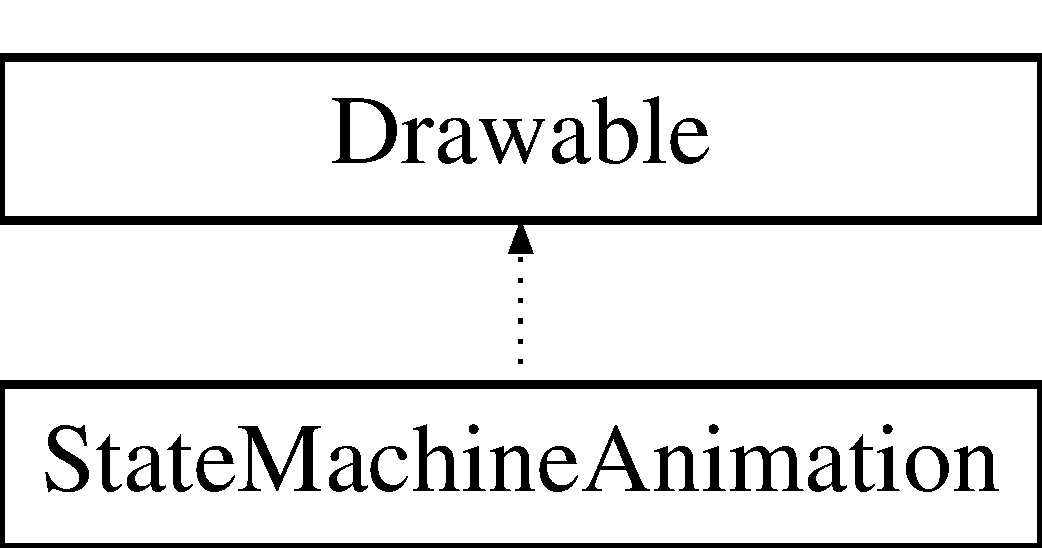
\includegraphics[height=2.000000cm]{classStateMachineAnimation}
\end{center}
\end{figure}
\subsection*{Métodos públicos}
\begin{DoxyCompactItemize}
\item 
\hyperlink{classStateMachineAnimation_ab3e0c7cea2112e3ae5a8093e3057a3b6}{State\+Machine\+Animation} (\hyperlink{classStateMachine}{State\+Machine} \&state\+Machine)
\item 
void \hyperlink{classStateMachineAnimation_aa2d5c955f19ec518080aa0cde7944473}{add\+Animation} (\hyperlink{classAnimation}{Animation} $\ast$animation)
\item 
void \hyperlink{classStateMachineAnimation_a8c715fbbaa26c4e52c72e074d27e2ea1}{update} (sf\+::\+Time delta)
\item 
void \hyperlink{classStateMachineAnimation_aadd7174f7f5aaa13d1a9889e5cc3539f}{update} (int action)
\item 
void \hyperlink{classStateMachineAnimation_a85f6a5c3b3963e9fd8767216ec0e735a}{update} (Actions action)
\item 
\hypertarget{classStateMachineAnimation_a717c4e5c86f7592acf43e5d4e184c002}{}virtual void {\bfseries draw} (sf\+::\+Render\+Target \&target, sf\+::\+Render\+States states) const \label{classStateMachineAnimation_a717c4e5c86f7592acf43e5d4e184c002}

\item 
void \hyperlink{classStateMachineAnimation_a4612f25e1bc04639bf7998fc6f90c23d}{set\+Animations} (std\+::vector$<$ \hyperlink{classAnimation}{Animation} $\ast$ $>$ $\ast$animations)
\end{DoxyCompactItemize}


\subsection{Descripción detallada}
Clase que representa una máquina de estados finitos y controla la animación que se esté reproduciendo en el momento 

\subsection{Documentación del constructor y destructor}
\hypertarget{classStateMachineAnimation_ab3e0c7cea2112e3ae5a8093e3057a3b6}{}\index{State\+Machine\+Animation@{State\+Machine\+Animation}!State\+Machine\+Animation@{State\+Machine\+Animation}}
\index{State\+Machine\+Animation@{State\+Machine\+Animation}!State\+Machine\+Animation@{State\+Machine\+Animation}}
\subsubsection[{State\+Machine\+Animation}]{\setlength{\rightskip}{0pt plus 5cm}State\+Machine\+Animation\+::\+State\+Machine\+Animation (
\begin{DoxyParamCaption}
\item[{{\bf State\+Machine} \&}]{state\+Machine}
\end{DoxyParamCaption}
)}\label{classStateMachineAnimation_ab3e0c7cea2112e3ae5a8093e3057a3b6}
Constructor 
\begin{DoxyParams}{Parámetros}
{\em state\+Machine} & \\
\hline
\end{DoxyParams}


\subsection{Documentación de las funciones miembro}
\hypertarget{classStateMachineAnimation_aa2d5c955f19ec518080aa0cde7944473}{}\index{State\+Machine\+Animation@{State\+Machine\+Animation}!add\+Animation@{add\+Animation}}
\index{add\+Animation@{add\+Animation}!State\+Machine\+Animation@{State\+Machine\+Animation}}
\subsubsection[{add\+Animation}]{\setlength{\rightskip}{0pt plus 5cm}void State\+Machine\+Animation\+::add\+Animation (
\begin{DoxyParamCaption}
\item[{{\bf Animation} $\ast$}]{animation}
\end{DoxyParamCaption}
)}\label{classStateMachineAnimation_aa2d5c955f19ec518080aa0cde7944473}
Añade una animación 
\begin{DoxyParams}{Parámetros}
{\em animation} & animación a añadir \\
\hline
\end{DoxyParams}
\hypertarget{classStateMachineAnimation_a4612f25e1bc04639bf7998fc6f90c23d}{}\index{State\+Machine\+Animation@{State\+Machine\+Animation}!set\+Animations@{set\+Animations}}
\index{set\+Animations@{set\+Animations}!State\+Machine\+Animation@{State\+Machine\+Animation}}
\subsubsection[{set\+Animations}]{\setlength{\rightskip}{0pt plus 5cm}void State\+Machine\+Animation\+::set\+Animations (
\begin{DoxyParamCaption}
\item[{std\+::vector$<$ {\bf Animation} $\ast$ $>$ $\ast$}]{animations}
\end{DoxyParamCaption}
)}\label{classStateMachineAnimation_a4612f25e1bc04639bf7998fc6f90c23d}
Setea el vector de animaciones de la máquina 
\begin{DoxyParams}{Parámetros}
{\em animations} & \\
\hline
\end{DoxyParams}
\hypertarget{classStateMachineAnimation_a8c715fbbaa26c4e52c72e074d27e2ea1}{}\index{State\+Machine\+Animation@{State\+Machine\+Animation}!update@{update}}
\index{update@{update}!State\+Machine\+Animation@{State\+Machine\+Animation}}
\subsubsection[{update}]{\setlength{\rightskip}{0pt plus 5cm}void State\+Machine\+Animation\+::update (
\begin{DoxyParamCaption}
\item[{sf\+::\+Time}]{delta}
\end{DoxyParamCaption}
)}\label{classStateMachineAnimation_a8c715fbbaa26c4e52c72e074d27e2ea1}
Actualiza la animación actual 
\begin{DoxyParams}{Parámetros}
{\em delta} & tiempo entre frame y frame \\
\hline
\end{DoxyParams}
\hypertarget{classStateMachineAnimation_aadd7174f7f5aaa13d1a9889e5cc3539f}{}\index{State\+Machine\+Animation@{State\+Machine\+Animation}!update@{update}}
\index{update@{update}!State\+Machine\+Animation@{State\+Machine\+Animation}}
\subsubsection[{update}]{\setlength{\rightskip}{0pt plus 5cm}void State\+Machine\+Animation\+::update (
\begin{DoxyParamCaption}
\item[{int}]{action}
\end{DoxyParamCaption}
)}\label{classStateMachineAnimation_aadd7174f7f5aaa13d1a9889e5cc3539f}
Actualiza la máquina de estados finitos con la entrada 
\begin{DoxyParams}{Parámetros}
{\em action} & entrada para la máquina \\
\hline
\end{DoxyParams}
\hypertarget{classStateMachineAnimation_a85f6a5c3b3963e9fd8767216ec0e735a}{}\index{State\+Machine\+Animation@{State\+Machine\+Animation}!update@{update}}
\index{update@{update}!State\+Machine\+Animation@{State\+Machine\+Animation}}
\subsubsection[{update}]{\setlength{\rightskip}{0pt plus 5cm}void State\+Machine\+Animation\+::update (
\begin{DoxyParamCaption}
\item[{Actions}]{action}
\end{DoxyParamCaption}
)\hspace{0.3cm}{\ttfamily [inline]}}\label{classStateMachineAnimation_a85f6a5c3b3963e9fd8767216ec0e735a}
Actualiza la máquina de estados finitos con la entrada 
\begin{DoxyParams}{Parámetros}
{\em action} & entrada para la máquina \\
\hline
\end{DoxyParams}


La documentación para esta clase fue generada a partir de los siguientes ficheros\+:\begin{DoxyCompactItemize}
\item 
State\+Machine\+Animation.\+h\item 
State\+Machine\+Animation.\+cpp\end{DoxyCompactItemize}

\hypertarget{classStateStack}{}\section{Referencia de la Clase State\+Stack}
\label{classStateStack}\index{State\+Stack@{State\+Stack}}


{\ttfamily \#include $<$State\+Stack.\+h$>$}

Diagrama de herencias de State\+Stack\begin{figure}[H]
\begin{center}
\leavevmode
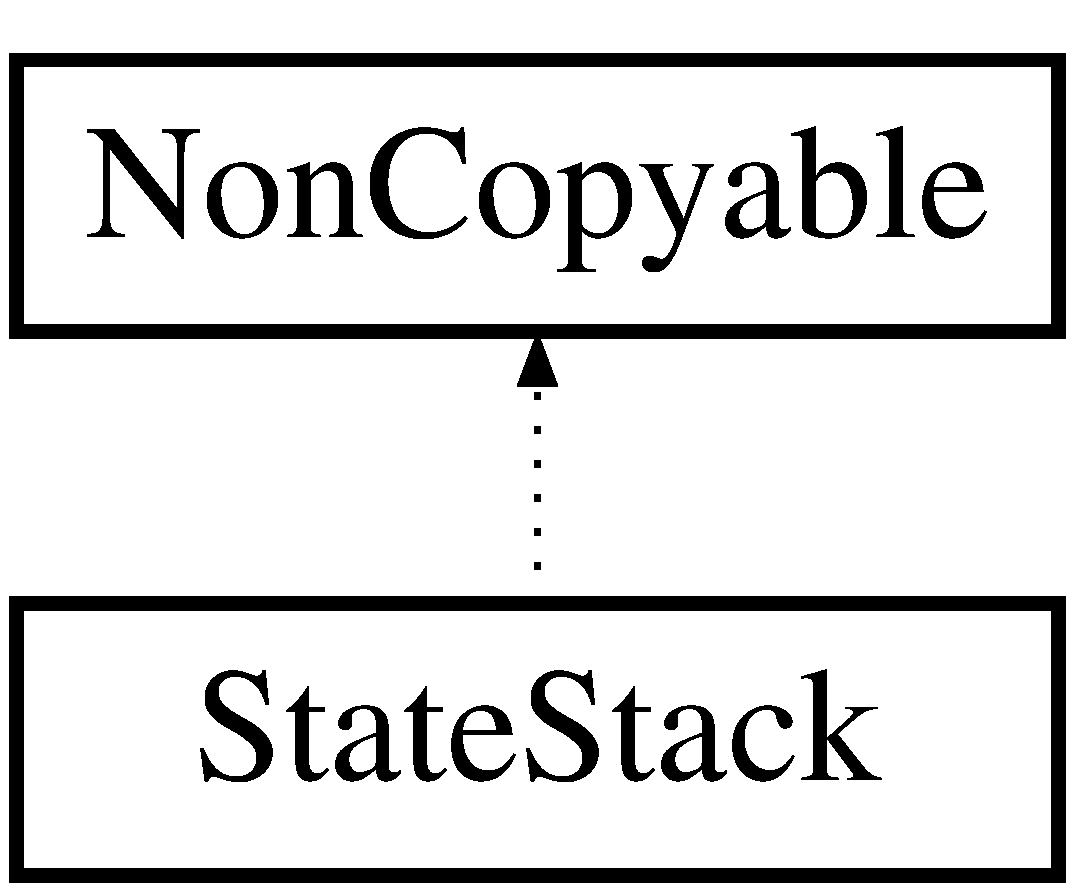
\includegraphics[height=2.000000cm]{classStateStack}
\end{center}
\end{figure}
\subsection*{Métodos públicos}
\begin{DoxyCompactItemize}
\item 
\hyperlink{classStateStack_a435529bdbbf2bc703997b8598767e9f4}{State\+Stack} (\hyperlink{classContext}{Context} context)
\item 
virtual \hyperlink{classStateStack_ab2d31c81756ff400d3edfac2a5c3456c}{$\sim$\+State\+Stack} ()
\item 
{\footnotesize template$<$typename T $>$ }\\void \hyperlink{classStateStack_a377470304b48fdd024ce37aaf5d2e127}{register\+State} (States\+I\+D state\+I\+D)
\item 
void \hyperlink{classStateStack_ae90af9f56ce7774d47d0407e2680c27d}{update} (sf\+::\+Time dt)
\item 
void \hyperlink{classStateStack_a0990b973b2a0bdf8fad2f326e564931a}{draw} ()
\item 
void \hyperlink{classStateStack_a70d3ffad9da499b8356789115f3e2acf}{handle\+Event} (const sf\+::\+Event \&event)
\item 
void \hyperlink{classStateStack_ac93b7e023e92a9bce352fce6e3ceecf0}{push\+State} (States\+I\+D state\+I\+D)
\item 
void \hyperlink{classStateStack_a7e050a57b798295c2344f1318765b5ee}{pop\+State} ()
\item 
void \hyperlink{classStateStack_a49f0703d4037c3bf63494e64cb09898d}{clear\+States} ()
\item 
bool \hyperlink{classStateStack_a63a73898d24eb0a68cac0215a9fda4fc}{is\+Empty} () const 
\end{DoxyCompactItemize}


\subsection{Descripción detallada}
Pila de estados 
\begin{DoxyParams}{Parámetros}
{\em context} & contexto de la aplicación \\
\hline
\end{DoxyParams}


\subsection{Documentación del constructor y destructor}
\hypertarget{classStateStack_a435529bdbbf2bc703997b8598767e9f4}{}\index{State\+Stack@{State\+Stack}!State\+Stack@{State\+Stack}}
\index{State\+Stack@{State\+Stack}!State\+Stack@{State\+Stack}}
\subsubsection[{State\+Stack}]{\setlength{\rightskip}{0pt plus 5cm}State\+Stack\+::\+State\+Stack (
\begin{DoxyParamCaption}
\item[{{\bf Context}}]{context}
\end{DoxyParamCaption}
)}\label{classStateStack_a435529bdbbf2bc703997b8598767e9f4}
Constructor 
\begin{DoxyParams}{Parámetros}
{\em context} & \\
\hline
\end{DoxyParams}
\hypertarget{classStateStack_ab2d31c81756ff400d3edfac2a5c3456c}{}\index{State\+Stack@{State\+Stack}!````~State\+Stack@{$\sim$\+State\+Stack}}
\index{````~State\+Stack@{$\sim$\+State\+Stack}!State\+Stack@{State\+Stack}}
\subsubsection[{$\sim$\+State\+Stack}]{\setlength{\rightskip}{0pt plus 5cm}State\+Stack\+::$\sim$\+State\+Stack (
\begin{DoxyParamCaption}
{}
\end{DoxyParamCaption}
)\hspace{0.3cm}{\ttfamily [virtual]}}\label{classStateStack_ab2d31c81756ff400d3edfac2a5c3456c}
Destructor 

\subsection{Documentación de las funciones miembro}
\hypertarget{classStateStack_a49f0703d4037c3bf63494e64cb09898d}{}\index{State\+Stack@{State\+Stack}!clear\+States@{clear\+States}}
\index{clear\+States@{clear\+States}!State\+Stack@{State\+Stack}}
\subsubsection[{clear\+States}]{\setlength{\rightskip}{0pt plus 5cm}void State\+Stack\+::clear\+States (
\begin{DoxyParamCaption}
{}
\end{DoxyParamCaption}
)}\label{classStateStack_a49f0703d4037c3bf63494e64cb09898d}
Limpia la pila de estados \hypertarget{classStateStack_a0990b973b2a0bdf8fad2f326e564931a}{}\index{State\+Stack@{State\+Stack}!draw@{draw}}
\index{draw@{draw}!State\+Stack@{State\+Stack}}
\subsubsection[{draw}]{\setlength{\rightskip}{0pt plus 5cm}void State\+Stack\+::draw (
\begin{DoxyParamCaption}
{}
\end{DoxyParamCaption}
)}\label{classStateStack_a0990b973b2a0bdf8fad2f326e564931a}
Dibuja los estados de la pila \hypertarget{classStateStack_a70d3ffad9da499b8356789115f3e2acf}{}\index{State\+Stack@{State\+Stack}!handle\+Event@{handle\+Event}}
\index{handle\+Event@{handle\+Event}!State\+Stack@{State\+Stack}}
\subsubsection[{handle\+Event}]{\setlength{\rightskip}{0pt plus 5cm}void State\+Stack\+::handle\+Event (
\begin{DoxyParamCaption}
\item[{const sf\+::\+Event \&}]{event}
\end{DoxyParamCaption}
)}\label{classStateStack_a70d3ffad9da499b8356789115f3e2acf}
Procesa los eventos delegándolos en los estados de la pila 
\begin{DoxyParams}{Parámetros}
{\em event} & \\
\hline
\end{DoxyParams}
\hypertarget{classStateStack_a63a73898d24eb0a68cac0215a9fda4fc}{}\index{State\+Stack@{State\+Stack}!is\+Empty@{is\+Empty}}
\index{is\+Empty@{is\+Empty}!State\+Stack@{State\+Stack}}
\subsubsection[{is\+Empty}]{\setlength{\rightskip}{0pt plus 5cm}bool State\+Stack\+::is\+Empty (
\begin{DoxyParamCaption}
{}
\end{DoxyParamCaption}
) const}\label{classStateStack_a63a73898d24eb0a68cac0215a9fda4fc}
Comprueba si la pila está vacía \begin{DoxyReturn}{Devuelve}
true si la pila está vacía 
\end{DoxyReturn}
\hypertarget{classStateStack_a7e050a57b798295c2344f1318765b5ee}{}\index{State\+Stack@{State\+Stack}!pop\+State@{pop\+State}}
\index{pop\+State@{pop\+State}!State\+Stack@{State\+Stack}}
\subsubsection[{pop\+State}]{\setlength{\rightskip}{0pt plus 5cm}void State\+Stack\+::pop\+State (
\begin{DoxyParamCaption}
{}
\end{DoxyParamCaption}
)}\label{classStateStack_a7e050a57b798295c2344f1318765b5ee}
Saca el último estado de la pila \hypertarget{classStateStack_ac93b7e023e92a9bce352fce6e3ceecf0}{}\index{State\+Stack@{State\+Stack}!push\+State@{push\+State}}
\index{push\+State@{push\+State}!State\+Stack@{State\+Stack}}
\subsubsection[{push\+State}]{\setlength{\rightskip}{0pt plus 5cm}void State\+Stack\+::push\+State (
\begin{DoxyParamCaption}
\item[{States\+I\+D}]{state\+I\+D}
\end{DoxyParamCaption}
)}\label{classStateStack_ac93b7e023e92a9bce352fce6e3ceecf0}
Coloca un estado en la pila 
\begin{DoxyParams}{Parámetros}
{\em state\+I\+D} & id del estado a colocar \\
\hline
\end{DoxyParams}
\hypertarget{classStateStack_a377470304b48fdd024ce37aaf5d2e127}{}\index{State\+Stack@{State\+Stack}!register\+State@{register\+State}}
\index{register\+State@{register\+State}!State\+Stack@{State\+Stack}}
\subsubsection[{register\+State}]{\setlength{\rightskip}{0pt plus 5cm}template$<$typename T $>$ void State\+Stack\+::register\+State (
\begin{DoxyParamCaption}
\item[{States\+I\+D}]{state\+I\+D}
\end{DoxyParamCaption}
)}\label{classStateStack_a377470304b48fdd024ce37aaf5d2e127}
Registra un estado en la pila 
\begin{DoxyParams}{Parámetros}
{\em state\+I\+D} & Plantilla para el registro de estados. Crea el estado que registra \\
\hline
{\em state\+I\+D} & identificador del estado \\
\hline
\end{DoxyParams}
\hypertarget{classStateStack_ae90af9f56ce7774d47d0407e2680c27d}{}\index{State\+Stack@{State\+Stack}!update@{update}}
\index{update@{update}!State\+Stack@{State\+Stack}}
\subsubsection[{update}]{\setlength{\rightskip}{0pt plus 5cm}void State\+Stack\+::update (
\begin{DoxyParamCaption}
\item[{sf\+::\+Time}]{dt}
\end{DoxyParamCaption}
)}\label{classStateStack_ae90af9f56ce7774d47d0407e2680c27d}
Actualiza los estados de la pila 
\begin{DoxyParams}{Parámetros}
{\em dt} & tiempo entre frame y frame \\
\hline
\end{DoxyParams}


La documentación para esta clase fue generada a partir de los siguientes ficheros\+:\begin{DoxyCompactItemize}
\item 
State\+Stack.\+h\item 
State\+Stack.\+cpp\end{DoxyCompactItemize}

\hypertarget{classStaticBlock}{}\section{Referencia de la Clase Static\+Block}
\label{classStaticBlock}\index{Static\+Block@{Static\+Block}}


{\ttfamily \#include $<$Static\+Block.\+h$>$}

Diagrama de herencias de Static\+Block\begin{figure}[H]
\begin{center}
\leavevmode
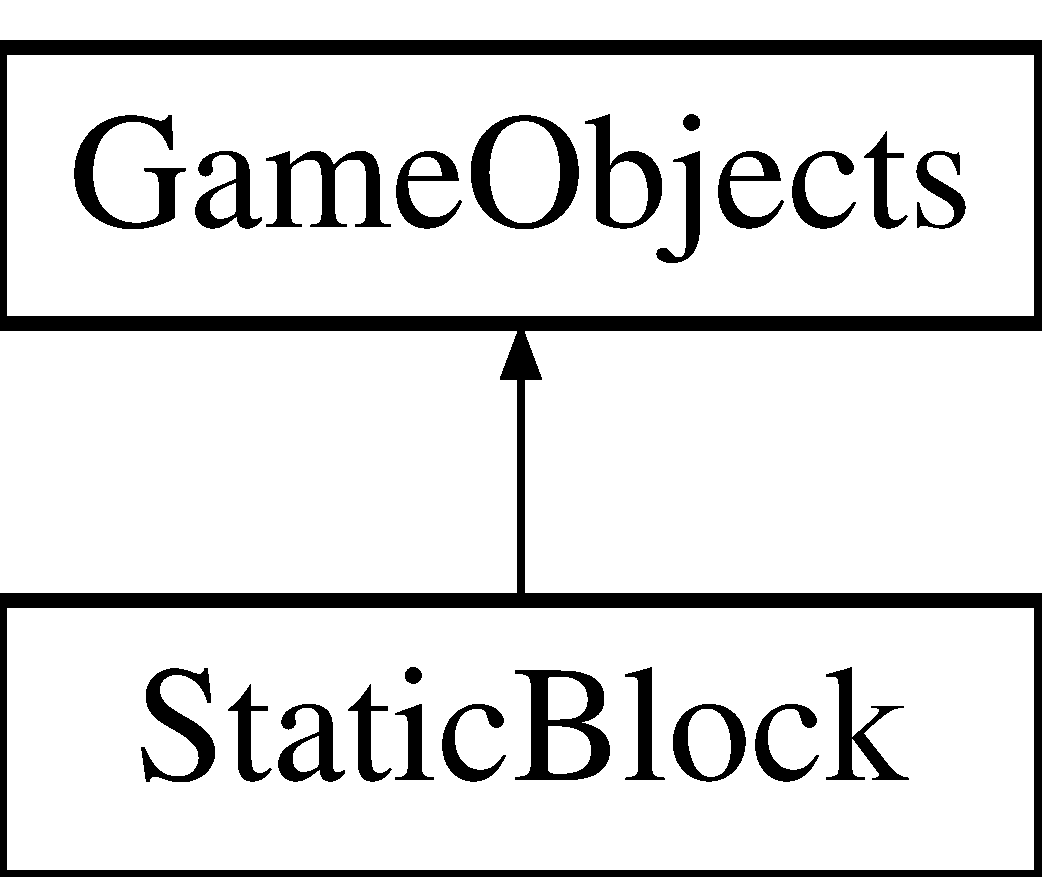
\includegraphics[height=2.000000cm]{classStaticBlock}
\end{center}
\end{figure}
\subsection*{Métodos públicos}
\begin{DoxyCompactItemize}
\item 
virtual \hyperlink{classEntity}{Entity} $\ast$ \hyperlink{classStaticBlock_a4443eba7de18fb6ee06fe40630ec22b8}{prepare\+Entity} (\hyperlink{classPropertyManager}{Property\+Manager} \&parameters)
\end{DoxyCompactItemize}


\subsection{Descripción detallada}
Constructor de una entidad concreta, un objeto del juego define un bloque transparente que no se puede atravesar 

\subsection{Documentación de las funciones miembro}
\hypertarget{classStaticBlock_a4443eba7de18fb6ee06fe40630ec22b8}{}\index{Static\+Block@{Static\+Block}!prepare\+Entity@{prepare\+Entity}}
\index{prepare\+Entity@{prepare\+Entity}!Static\+Block@{Static\+Block}}
\subsubsection[{prepare\+Entity}]{\setlength{\rightskip}{0pt plus 5cm}{\bf Entity} $\ast$ Static\+Block\+::prepare\+Entity (
\begin{DoxyParamCaption}
\item[{{\bf Property\+Manager} \&}]{parameters}
\end{DoxyParamCaption}
)\hspace{0.3cm}{\ttfamily [virtual]}}\label{classStaticBlock_a4443eba7de18fb6ee06fe40630ec22b8}
Devuelve una entidad que define un bloque invisible que no se puede atravesar dado unos parámetros 
\begin{DoxyParams}{Parámetros}
{\em parameters} & conjunto de parámetros \\
\hline
\end{DoxyParams}
\begin{DoxyReturn}{Devuelve}
entidad formada 
\end{DoxyReturn}


Implementa \hyperlink{classGameObjects_ad8d8177b229922b5a29e7355c8cf54ca}{Game\+Objects}.



La documentación para esta clase fue generada a partir de los siguientes ficheros\+:\begin{DoxyCompactItemize}
\item 
Static\+Block.\+h\item 
Static\+Block.\+cpp\end{DoxyCompactItemize}

\hypertarget{structStructAnimation}{}\section{Referencia de la Estructura Struct\+Animation}
\label{structStructAnimation}\index{Struct\+Animation@{Struct\+Animation}}


{\ttfamily \#include $<$Struct\+Animation.\+h$>$}

\subsection*{Campos de datos}
\begin{DoxyCompactItemize}
\item 
\hypertarget{structStructAnimation_a0373170e287c41c66499d16d1dd6e317}{}std\+::vector$<$ \hyperlink{classAnimation}{Animation} $\ast$ $>$ $\ast$ {\bfseries animations}\label{structStructAnimation_a0373170e287c41c66499d16d1dd6e317}

\end{DoxyCompactItemize}


\subsection{Descripción detallada}
Estructura para guardar información sobre animaciones 

La documentación para esta estructura fue generada a partir del siguiente fichero\+:\begin{DoxyCompactItemize}
\item 
Struct\+Animation.\+h\end{DoxyCompactItemize}

\hypertarget{structStructCollision}{}\section{Referencia de la Estructura Struct\+Collision}
\label{structStructCollision}\index{Struct\+Collision@{Struct\+Collision}}


{\ttfamily \#include $<$Struct\+Collision.\+h$>$}

\subsection*{Campos de datos}
\begin{DoxyCompactItemize}
\item 
\hypertarget{structStructCollision_a3b1bd19764801e168270763ce704523d}{}sf\+::\+Vertex\+Array $\ast$ {\bfseries vertices}\label{structStructCollision_a3b1bd19764801e168270763ce704523d}

\item 
\hypertarget{structStructCollision_a6f7f524aeef17b95b36e4d60dae2435a}{}std\+::string {\bfseries type\+Collision}\label{structStructCollision_a6f7f524aeef17b95b36e4d60dae2435a}

\item 
\hypertarget{structStructCollision_a43eba21f8c0c121d1a5f5693f7739119}{}sf\+::\+Vector2f {\bfseries position}\label{structStructCollision_a43eba21f8c0c121d1a5f5693f7739119}

\item 
\hypertarget{structStructCollision_a8b9b225135398133220aeffa1cc8fd18}{}std\+::string $\ast$ {\bfseries data}\label{structStructCollision_a8b9b225135398133220aeffa1cc8fd18}

\end{DoxyCompactItemize}


\subsection{Descripción detallada}
Estructura para guardar información de colisiones 

La documentación para esta estructura fue generada a partir del siguiente fichero\+:\begin{DoxyCompactItemize}
\item 
Struct\+Collision.\+h\end{DoxyCompactItemize}

\hypertarget{structStructMap}{}\section{Referencia de la Estructura Struct\+Map}
\label{structStructMap}\index{Struct\+Map@{Struct\+Map}}


{\ttfamily \#include $<$Struct\+Map.\+h$>$}

\subsection*{Campos de datos}
\begin{DoxyCompactItemize}
\item 
\hypertarget{structStructMap_a64118a2afb5e259600f5c8412c97931a}{}int {\bfseries number\+Columns}\label{structStructMap_a64118a2afb5e259600f5c8412c97931a}

\item 
\hypertarget{structStructMap_a85d452fd6408616208edf76c4e8f2903}{}int {\bfseries number\+Rows}\label{structStructMap_a85d452fd6408616208edf76c4e8f2903}

\item 
\hypertarget{structStructMap_a3839f140fb8b2795554f855c18a20fdb}{}int {\bfseries tile\+Height}\label{structStructMap_a3839f140fb8b2795554f855c18a20fdb}

\item 
\hypertarget{structStructMap_a32790590928447bdcf6a5d8ca63d22be}{}int {\bfseries tile\+Width}\label{structStructMap_a32790590928447bdcf6a5d8ca63d22be}

\item 
\hypertarget{structStructMap_af71fbbc4cb1dff2825ba92e6e333e7e9}{}int $\ast$ {\bfseries tiles}\label{structStructMap_af71fbbc4cb1dff2825ba92e6e333e7e9}

\item 
\hypertarget{structStructMap_a4cb80a51771af2fd3ab061da75a7db00}{}std\+::vector$<$ sf\+::\+Vector3i $>$ $\ast$ {\bfseries underground}\label{structStructMap_a4cb80a51771af2fd3ab061da75a7db00}

\end{DoxyCompactItemize}


\subsection{Descripción detallada}
Estructura para guardar información de tiles de un mapa 

La documentación para esta estructura fue generada a partir de los siguientes ficheros\+:\begin{DoxyCompactItemize}
\item 
Struct\+Map.\+h\item 
Struct\+Map.\+cpp\end{DoxyCompactItemize}

\hypertarget{structStructPeople}{}\section{Referencia de la Estructura Struct\+People}
\label{structStructPeople}\index{Struct\+People@{Struct\+People}}


{\ttfamily \#include $<$Struct\+People.\+h$>$}

\subsection*{Campos de datos}
\begin{DoxyCompactItemize}
\item 
\hypertarget{structStructPeople_a9beb4fd84ea9b068b982a6217847b194}{}std\+::vector$<$ std\+::string $\ast$ $>$ $\ast$ {\bfseries villagers}\label{structStructPeople_a9beb4fd84ea9b068b982a6217847b194}

\item 
\hypertarget{structStructPeople_ae6278812dfcc4a951ebdffec5fb444dd}{}std\+::string $\ast$ {\bfseries character}\label{structStructPeople_ae6278812dfcc4a951ebdffec5fb444dd}

\end{DoxyCompactItemize}


\subsection{Descripción detallada}
Estructura para guardar los id del protagonista y de aldeanos que hay en un mapa 

La documentación para esta estructura fue generada a partir de los siguientes ficheros\+:\begin{DoxyCompactItemize}
\item 
Struct\+People.\+h\item 
Struct\+People.\+cpp\end{DoxyCompactItemize}

\hypertarget{classSubject}{}\section{Referencia de la Clase Subject}
\label{classSubject}\index{Subject@{Subject}}


{\ttfamily \#include $<$Subject.\+h$>$}

\subsection*{Métodos públicos}
\begin{DoxyCompactItemize}
\item 
\hyperlink{classSubject_ab468044832c824c6d6c2f46272655207}{Subject} ()
\item 
void \hyperlink{classSubject_aec0d2f94b266d79c426b0ac454d823a5}{attach} (\hyperlink{classObserver}{Observer} $\ast$obs)
\item 
void \hyperlink{classSubject_ad101324d66ad30b943e4fdc31dc16d14}{detach} (\hyperlink{classObserver}{Observer} $\ast$obs)
\item 
void \hyperlink{classSubject_ae24f8fe7039fed0caa2acd3790a6b9c4}{set\+Message} (\hyperlink{classMessage}{Message} \&val)
\item 
\hyperlink{classMessage}{Message} \hyperlink{classSubject_ad9798f18a9947694b11be57e72d80f12}{get\+Message} ()
\item 
void \hyperlink{classSubject_af104c2baf37c7aa63b2ef6d32c2b3a9c}{notify} ()
\end{DoxyCompactItemize}


\subsection{Descripción detallada}
Clase vigilada por los observadores en el patrón observer 

\subsection{Documentación del constructor y destructor}
\hypertarget{classSubject_ab468044832c824c6d6c2f46272655207}{}\index{Subject@{Subject}!Subject@{Subject}}
\index{Subject@{Subject}!Subject@{Subject}}
\subsubsection[{Subject}]{\setlength{\rightskip}{0pt plus 5cm}Subject\+::\+Subject (
\begin{DoxyParamCaption}
{}
\end{DoxyParamCaption}
)\hspace{0.3cm}{\ttfamily [inline]}}\label{classSubject_ab468044832c824c6d6c2f46272655207}
Constructor por defecto 

\subsection{Documentación de las funciones miembro}
\hypertarget{classSubject_aec0d2f94b266d79c426b0ac454d823a5}{}\index{Subject@{Subject}!attach@{attach}}
\index{attach@{attach}!Subject@{Subject}}
\subsubsection[{attach}]{\setlength{\rightskip}{0pt plus 5cm}void Subject\+::attach (
\begin{DoxyParamCaption}
\item[{{\bf Observer} $\ast$}]{obs}
\end{DoxyParamCaption}
)\hspace{0.3cm}{\ttfamily [inline]}}\label{classSubject_aec0d2f94b266d79c426b0ac454d823a5}
Guarda un observador 
\begin{DoxyParams}{Parámetros}
{\em obs} & observador \\
\hline
\end{DoxyParams}
\hypertarget{classSubject_ad101324d66ad30b943e4fdc31dc16d14}{}\index{Subject@{Subject}!detach@{detach}}
\index{detach@{detach}!Subject@{Subject}}
\subsubsection[{detach}]{\setlength{\rightskip}{0pt plus 5cm}void Subject\+::detach (
\begin{DoxyParamCaption}
\item[{{\bf Observer} $\ast$}]{obs}
\end{DoxyParamCaption}
)\hspace{0.3cm}{\ttfamily [inline]}}\label{classSubject_ad101324d66ad30b943e4fdc31dc16d14}
Quita un observador 
\begin{DoxyParams}{Parámetros}
{\em obs} & observador a quitar \\
\hline
\end{DoxyParams}
\hypertarget{classSubject_ad9798f18a9947694b11be57e72d80f12}{}\index{Subject@{Subject}!get\+Message@{get\+Message}}
\index{get\+Message@{get\+Message}!Subject@{Subject}}
\subsubsection[{get\+Message}]{\setlength{\rightskip}{0pt plus 5cm}{\bf Message} Subject\+::get\+Message (
\begin{DoxyParamCaption}
{}
\end{DoxyParamCaption}
)\hspace{0.3cm}{\ttfamily [inline]}}\label{classSubject_ad9798f18a9947694b11be57e72d80f12}
Devuelve el mensaje \begin{DoxyReturn}{Devuelve}
mensaje 
\end{DoxyReturn}
\hypertarget{classSubject_af104c2baf37c7aa63b2ef6d32c2b3a9c}{}\index{Subject@{Subject}!notify@{notify}}
\index{notify@{notify}!Subject@{Subject}}
\subsubsection[{notify}]{\setlength{\rightskip}{0pt plus 5cm}void Subject\+::notify (
\begin{DoxyParamCaption}
{}
\end{DoxyParamCaption}
)}\label{classSubject_af104c2baf37c7aa63b2ef6d32c2b3a9c}
Notifica a los observadores de cambios \hypertarget{classSubject_ae24f8fe7039fed0caa2acd3790a6b9c4}{}\index{Subject@{Subject}!set\+Message@{set\+Message}}
\index{set\+Message@{set\+Message}!Subject@{Subject}}
\subsubsection[{set\+Message}]{\setlength{\rightskip}{0pt plus 5cm}void Subject\+::set\+Message (
\begin{DoxyParamCaption}
\item[{{\bf Message} \&}]{val}
\end{DoxyParamCaption}
)\hspace{0.3cm}{\ttfamily [inline]}}\label{classSubject_ae24f8fe7039fed0caa2acd3790a6b9c4}
Setea el mensaje y notifica a los observadores 
\begin{DoxyParams}{Parámetros}
{\em val} & mensaje a setear \\
\hline
\end{DoxyParams}


La documentación para esta clase fue generada a partir de los siguientes ficheros\+:\begin{DoxyCompactItemize}
\item 
Subject.\+h\item 
Subject.\+cpp\end{DoxyCompactItemize}

\hypertarget{classSubStateGame}{}\section{Referencia de la Clase Sub\+State\+Game}
\label{classSubStateGame}\index{Sub\+State\+Game@{Sub\+State\+Game}}


{\ttfamily \#include $<$Sub\+State\+Game.\+h$>$}

Diagrama de herencias de Sub\+State\+Game\begin{figure}[H]
\begin{center}
\leavevmode
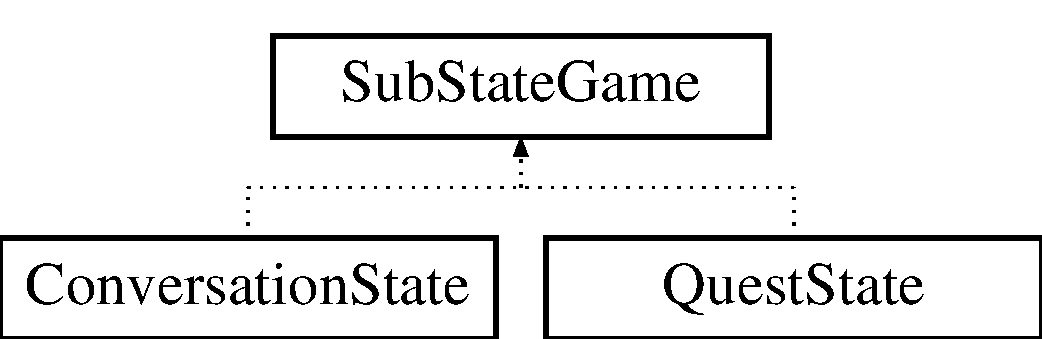
\includegraphics[height=2.000000cm]{classSubStateGame}
\end{center}
\end{figure}
\subsection*{Métodos públicos}
\begin{DoxyCompactItemize}
\item 
\hypertarget{classSubStateGame_a63176b9e97fa67b25609bed1c1810e95}{}virtual void {\bfseries draw} ()=0\label{classSubStateGame_a63176b9e97fa67b25609bed1c1810e95}

\item 
\hypertarget{classSubStateGame_af8e401cd2b5032e2d677eaac6bff3253}{}virtual bool {\bfseries update} (sf\+::\+Time delta)=0\label{classSubStateGame_af8e401cd2b5032e2d677eaac6bff3253}

\item 
\hypertarget{classSubStateGame_af4ebe86d83d064a02049160915c4ac97}{}virtual bool {\bfseries handle\+Event} (const sf\+::\+Event \&event)=0\label{classSubStateGame_af4ebe86d83d064a02049160915c4ac97}

\item 
void \hyperlink{classSubStateGame_ad50890e351e9ca02fec294bd3139e887}{set\+Ended} ()
\item 
bool \hyperlink{classSubStateGame_ac5bf0c28ce1a5f2de71246dd4dc4fc0e}{is\+Ended} () const 
\end{DoxyCompactItemize}


\subsection{Descripción detallada}
Clase base para los subestados del juego 

\subsection{Documentación de las funciones miembro}
\hypertarget{classSubStateGame_ac5bf0c28ce1a5f2de71246dd4dc4fc0e}{}\index{Sub\+State\+Game@{Sub\+State\+Game}!is\+Ended@{is\+Ended}}
\index{is\+Ended@{is\+Ended}!Sub\+State\+Game@{Sub\+State\+Game}}
\subsubsection[{is\+Ended}]{\setlength{\rightskip}{0pt plus 5cm}bool Sub\+State\+Game\+::is\+Ended (
\begin{DoxyParamCaption}
{}
\end{DoxyParamCaption}
) const\hspace{0.3cm}{\ttfamily [inline]}}\label{classSubStateGame_ac5bf0c28ce1a5f2de71246dd4dc4fc0e}
Devuelve si el subestado del juego ha terminado \begin{DoxyReturn}{Devuelve}
true si ha terminado 
\end{DoxyReturn}
\hypertarget{classSubStateGame_ad50890e351e9ca02fec294bd3139e887}{}\index{Sub\+State\+Game@{Sub\+State\+Game}!set\+Ended@{set\+Ended}}
\index{set\+Ended@{set\+Ended}!Sub\+State\+Game@{Sub\+State\+Game}}
\subsubsection[{set\+Ended}]{\setlength{\rightskip}{0pt plus 5cm}void Sub\+State\+Game\+::set\+Ended (
\begin{DoxyParamCaption}
{}
\end{DoxyParamCaption}
)\hspace{0.3cm}{\ttfamily [inline]}}\label{classSubStateGame_ad50890e351e9ca02fec294bd3139e887}
Setea si el subestado ha terminado 

La documentación para esta clase fue generada a partir del siguiente fichero\+:\begin{DoxyCompactItemize}
\item 
Sub\+State\+Game.\+h\end{DoxyCompactItemize}

\hypertarget{classSystemCollision}{}\section{Referencia de la Clase System\+Collision}
\label{classSystemCollision}\index{System\+Collision@{System\+Collision}}


{\ttfamily \#include $<$System\+Collision.\+h$>$}

Diagrama de herencias de System\+Collision\begin{figure}[H]
\begin{center}
\leavevmode
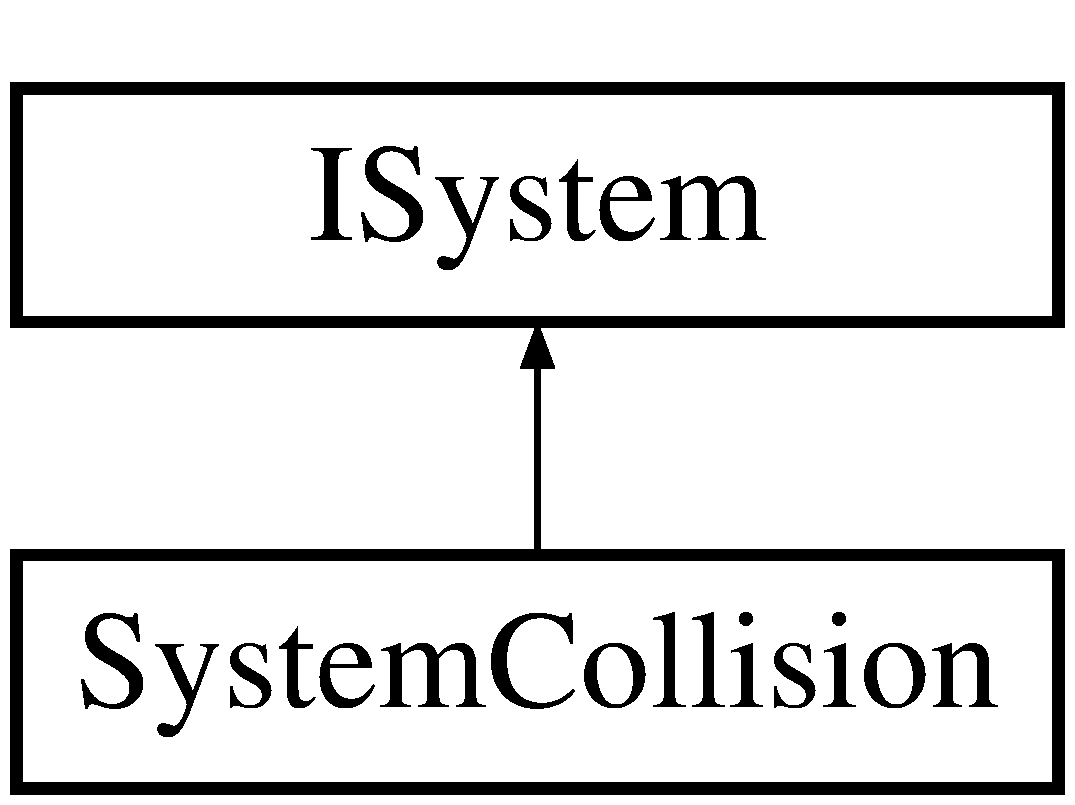
\includegraphics[height=2.000000cm]{classSystemCollision}
\end{center}
\end{figure}
\subsection*{Métodos públicos}
\begin{DoxyCompactItemize}
\item 
\hyperlink{classSystemCollision_a32a9ae61fbeda597cdd3e8cf991782f6}{System\+Collision} (sf\+::\+Float\+Rect bounds)
\item 
virtual void \hyperlink{classSystemCollision_ab2ced8fd115cd326a29a3535ddba7367}{initialize} ()
\item 
virtual void \hyperlink{classSystemCollision_a8c8ae9c8bb8f9f69e4b656c4ff496a30}{finalize} ()
\item 
virtual void \hyperlink{classSystemCollision_ab2dae21a0636bf6d24c6fd7f596f07d1}{update} (sf\+::\+Time dt)
\item 
virtual void \hyperlink{classSystemCollision_a731cd70ffedfa221454348ad975ee82c}{update\+Second\+Part} (sf\+::\+Time dt)
\item 
virtual void \hyperlink{classSystemCollision_a228a39b4c9bc3d6b7934a25814acda7a}{register\+Entity} (\hyperlink{classEntity}{Entity} $\ast$entity)
\item 
virtual void \hyperlink{classSystemCollision_a8890b0a585ac5e9a99510839a9713de4}{removed\+Entity} (\hyperlink{classEntity}{Entity} $\ast$entity)
\item 
void \hyperlink{classSystemCollision_a87344c57cc07fbc29741a8f0bf6f71ba}{new\+World\+Collision} (sf\+::\+Float\+Rect bounds)
\item 
void \hyperlink{classSystemCollision_a588abcc7ca31e3f2e23a16165f62b74d}{clear} ()
\item 
std\+::vector$<$ \hyperlink{classEntity}{Entity} $\ast$ $>$ $\ast$ \hyperlink{classSystemCollision_ac9b0781fe501dd70ce28037230a6574f}{query} (sf\+::\+Float\+Rect query)
\item 
void \hyperlink{classSystemCollision_afa60781f0a681875d053275eb78a13c9}{check\+Collisions} (sf\+::\+Float\+Rect region)
\item 
void \hyperlink{classSystemCollision_acbc4c623f1f4dd9c6def15013498ed3d}{correct\+Inside\+Position} (\hyperlink{classEntity}{Entity} $\ast$entity)
\item 
void \hyperlink{classSystemCollision_a90b827486b7e03081af461970a799adb}{resolve\+Collisions} ()
\end{DoxyCompactItemize}
\subsection*{Otros miembros heredados}


\subsection{Descripción detallada}
Sistema de colisiones 

\subsection{Documentación del constructor y destructor}
\hypertarget{classSystemCollision_a32a9ae61fbeda597cdd3e8cf991782f6}{}\index{System\+Collision@{System\+Collision}!System\+Collision@{System\+Collision}}
\index{System\+Collision@{System\+Collision}!System\+Collision@{System\+Collision}}
\subsubsection[{System\+Collision}]{\setlength{\rightskip}{0pt plus 5cm}System\+Collision\+::\+System\+Collision (
\begin{DoxyParamCaption}
\item[{sf\+::\+Float\+Rect}]{bounds}
\end{DoxyParamCaption}
)}\label{classSystemCollision_a32a9ae61fbeda597cdd3e8cf991782f6}
Constructor. Se le pasa los límites del mapa 
\begin{DoxyParams}{Parámetros}
{\em bounds} & limites del mapa \\
\hline
\end{DoxyParams}


\subsection{Documentación de las funciones miembro}
\hypertarget{classSystemCollision_afa60781f0a681875d053275eb78a13c9}{}\index{System\+Collision@{System\+Collision}!check\+Collisions@{check\+Collisions}}
\index{check\+Collisions@{check\+Collisions}!System\+Collision@{System\+Collision}}
\subsubsection[{check\+Collisions}]{\setlength{\rightskip}{0pt plus 5cm}void System\+Collision\+::check\+Collisions (
\begin{DoxyParamCaption}
\item[{sf\+::\+Float\+Rect}]{region}
\end{DoxyParamCaption}
)}\label{classSystemCollision_afa60781f0a681875d053275eb78a13c9}
Checkea todas las colisiones que se producen en la región dada las va guardando en una pila 
\begin{DoxyParams}{Parámetros}
{\em region} & zona a consultar colisiones \\
\hline
\end{DoxyParams}
\hypertarget{classSystemCollision_a588abcc7ca31e3f2e23a16165f62b74d}{}\index{System\+Collision@{System\+Collision}!clear@{clear}}
\index{clear@{clear}!System\+Collision@{System\+Collision}}
\subsubsection[{clear}]{\setlength{\rightskip}{0pt plus 5cm}void System\+Collision\+::clear (
\begin{DoxyParamCaption}
{}
\end{DoxyParamCaption}
)}\label{classSystemCollision_a588abcc7ca31e3f2e23a16165f62b74d}
Limpia el mundo colisionable \hypertarget{classSystemCollision_acbc4c623f1f4dd9c6def15013498ed3d}{}\index{System\+Collision@{System\+Collision}!correct\+Inside\+Position@{correct\+Inside\+Position}}
\index{correct\+Inside\+Position@{correct\+Inside\+Position}!System\+Collision@{System\+Collision}}
\subsubsection[{correct\+Inside\+Position}]{\setlength{\rightskip}{0pt plus 5cm}void System\+Collision\+::correct\+Inside\+Position (
\begin{DoxyParamCaption}
\item[{{\bf Entity} $\ast$}]{entity}
\end{DoxyParamCaption}
)}\label{classSystemCollision_acbc4c623f1f4dd9c6def15013498ed3d}
mantiene la entidad dentro del mundo, sin que se salga de los límites lo corrige si es necesario 
\begin{DoxyParams}{Parámetros}
{\em entity} & entidad a comprobar \\
\hline
\end{DoxyParams}
\hypertarget{classSystemCollision_a8c8ae9c8bb8f9f69e4b656c4ff496a30}{}\index{System\+Collision@{System\+Collision}!finalize@{finalize}}
\index{finalize@{finalize}!System\+Collision@{System\+Collision}}
\subsubsection[{finalize}]{\setlength{\rightskip}{0pt plus 5cm}void System\+Collision\+::finalize (
\begin{DoxyParamCaption}
{}
\end{DoxyParamCaption}
)\hspace{0.3cm}{\ttfamily [virtual]}}\label{classSystemCollision_a8c8ae9c8bb8f9f69e4b656c4ff496a30}
Finaliza el sistema 

Reimplementado de \hyperlink{classISystem_a4cc1cac06100c45d260a23d24d5618d6}{I\+System}.

\hypertarget{classSystemCollision_ab2ced8fd115cd326a29a3535ddba7367}{}\index{System\+Collision@{System\+Collision}!initialize@{initialize}}
\index{initialize@{initialize}!System\+Collision@{System\+Collision}}
\subsubsection[{initialize}]{\setlength{\rightskip}{0pt plus 5cm}virtual void System\+Collision\+::initialize (
\begin{DoxyParamCaption}
{}
\end{DoxyParamCaption}
)\hspace{0.3cm}{\ttfamily [inline]}, {\ttfamily [virtual]}}\label{classSystemCollision_ab2ced8fd115cd326a29a3535ddba7367}
Inicializa el sistema 

Reimplementado de \hyperlink{classISystem_ac9b257acd7d03dbd7aab149792ff98af}{I\+System}.

\hypertarget{classSystemCollision_a87344c57cc07fbc29741a8f0bf6f71ba}{}\index{System\+Collision@{System\+Collision}!new\+World\+Collision@{new\+World\+Collision}}
\index{new\+World\+Collision@{new\+World\+Collision}!System\+Collision@{System\+Collision}}
\subsubsection[{new\+World\+Collision}]{\setlength{\rightskip}{0pt plus 5cm}void System\+Collision\+::new\+World\+Collision (
\begin{DoxyParamCaption}
\item[{sf\+::\+Float\+Rect}]{bounds}
\end{DoxyParamCaption}
)}\label{classSystemCollision_a87344c57cc07fbc29741a8f0bf6f71ba}
Crea un nuevo mundo colisionable 
\begin{DoxyParams}{Parámetros}
{\em bounds} & nuevos limites del mapa \\
\hline
\end{DoxyParams}
\hypertarget{classSystemCollision_ac9b0781fe501dd70ce28037230a6574f}{}\index{System\+Collision@{System\+Collision}!query@{query}}
\index{query@{query}!System\+Collision@{System\+Collision}}
\subsubsection[{query}]{\setlength{\rightskip}{0pt plus 5cm}std\+::vector$<$ {\bf Entity} $\ast$ $>$ $\ast$ System\+Collision\+::query (
\begin{DoxyParamCaption}
\item[{sf\+::\+Float\+Rect}]{query}
\end{DoxyParamCaption}
)}\label{classSystemCollision_ac9b0781fe501dd70ce28037230a6574f}
Busca todas las entidades que colisionan con el cuadrado dado 
\begin{DoxyParams}{Parámetros}
{\em query} & zona a consultar \\
\hline
\end{DoxyParams}
\begin{DoxyReturn}{Devuelve}
lista de entidades que colisionan 
\end{DoxyReturn}
\hypertarget{classSystemCollision_a228a39b4c9bc3d6b7934a25814acda7a}{}\index{System\+Collision@{System\+Collision}!register\+Entity@{register\+Entity}}
\index{register\+Entity@{register\+Entity}!System\+Collision@{System\+Collision}}
\subsubsection[{register\+Entity}]{\setlength{\rightskip}{0pt plus 5cm}void System\+Collision\+::register\+Entity (
\begin{DoxyParamCaption}
\item[{{\bf Entity} $\ast$}]{entity}
\end{DoxyParamCaption}
)\hspace{0.3cm}{\ttfamily [virtual]}}\label{classSystemCollision_a228a39b4c9bc3d6b7934a25814acda7a}
Registra una entidad en el sistema si es de su incumbencia 
\begin{DoxyParams}{Parámetros}
{\em entity} & entidad a registrar \\
\hline
\end{DoxyParams}


Implementa \hyperlink{classISystem_aaaef32b093b566b0573cb23e00f8c7ae}{I\+System}.

\hypertarget{classSystemCollision_a8890b0a585ac5e9a99510839a9713de4}{}\index{System\+Collision@{System\+Collision}!removed\+Entity@{removed\+Entity}}
\index{removed\+Entity@{removed\+Entity}!System\+Collision@{System\+Collision}}
\subsubsection[{removed\+Entity}]{\setlength{\rightskip}{0pt plus 5cm}void System\+Collision\+::removed\+Entity (
\begin{DoxyParamCaption}
\item[{{\bf Entity} $\ast$}]{entity}
\end{DoxyParamCaption}
)\hspace{0.3cm}{\ttfamily [virtual]}}\label{classSystemCollision_a8890b0a585ac5e9a99510839a9713de4}
Elimina la entidad del sistema 
\begin{DoxyParams}{Parámetros}
{\em entity} & \\
\hline
\end{DoxyParams}


Implementa \hyperlink{classISystem_a0e966d506838cfe09543ad4ccafa4998}{I\+System}.

\hypertarget{classSystemCollision_a90b827486b7e03081af461970a799adb}{}\index{System\+Collision@{System\+Collision}!resolve\+Collisions@{resolve\+Collisions}}
\index{resolve\+Collisions@{resolve\+Collisions}!System\+Collision@{System\+Collision}}
\subsubsection[{resolve\+Collisions}]{\setlength{\rightskip}{0pt plus 5cm}void System\+Collision\+::resolve\+Collisions (
\begin{DoxyParamCaption}
{}
\end{DoxyParamCaption}
)}\label{classSystemCollision_a90b827486b7e03081af461970a799adb}
Resuelve las colisiones que han quedado en la cola después de comprobar, son delegados en las entidades \hypertarget{classSystemCollision_ab2dae21a0636bf6d24c6fd7f596f07d1}{}\index{System\+Collision@{System\+Collision}!update@{update}}
\index{update@{update}!System\+Collision@{System\+Collision}}
\subsubsection[{update}]{\setlength{\rightskip}{0pt plus 5cm}void System\+Collision\+::update (
\begin{DoxyParamCaption}
\item[{sf\+::\+Time}]{dt}
\end{DoxyParamCaption}
)\hspace{0.3cm}{\ttfamily [virtual]}}\label{classSystemCollision_ab2dae21a0636bf6d24c6fd7f596f07d1}
Actualiza el sistema en una primera tanda 
\begin{DoxyParams}{Parámetros}
{\em dt} & tiempo entre frame y frame \\
\hline
\end{DoxyParams}


Reimplementado de \hyperlink{classISystem_a6931efd2517fd0c81237beeb04297421}{I\+System}.

\hypertarget{classSystemCollision_a731cd70ffedfa221454348ad975ee82c}{}\index{System\+Collision@{System\+Collision}!update\+Second\+Part@{update\+Second\+Part}}
\index{update\+Second\+Part@{update\+Second\+Part}!System\+Collision@{System\+Collision}}
\subsubsection[{update\+Second\+Part}]{\setlength{\rightskip}{0pt plus 5cm}void System\+Collision\+::update\+Second\+Part (
\begin{DoxyParamCaption}
\item[{sf\+::\+Time}]{dt}
\end{DoxyParamCaption}
)\hspace{0.3cm}{\ttfamily [virtual]}}\label{classSystemCollision_a731cd70ffedfa221454348ad975ee82c}
Actualiza el sistema en una segunda tanda 
\begin{DoxyParams}{Parámetros}
{\em dt} & tiempo entre frame y frame \\
\hline
\end{DoxyParams}


Reimplementado de \hyperlink{classISystem_aef2545bd6ffac18186b566e4d3d2804b}{I\+System}.



La documentación para esta clase fue generada a partir de los siguientes ficheros\+:\begin{DoxyCompactItemize}
\item 
System\+Collision.\+h\item 
System\+Collision.\+cpp\end{DoxyCompactItemize}

\hypertarget{classSystemCommand}{}\section{Referencia de la Clase System\+Command}
\label{classSystemCommand}\index{System\+Command@{System\+Command}}


{\ttfamily \#include $<$System\+Command.\+h$>$}

Diagrama de herencias de System\+Command\begin{figure}[H]
\begin{center}
\leavevmode
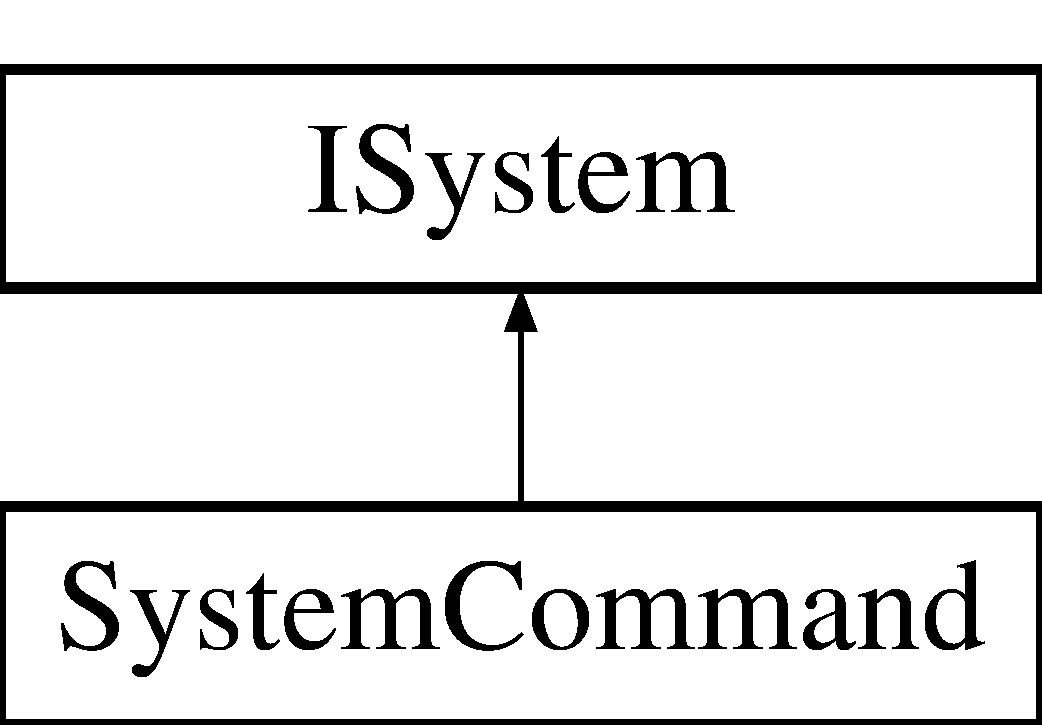
\includegraphics[height=2.000000cm]{classSystemCommand}
\end{center}
\end{figure}
\subsection*{Métodos públicos}
\begin{DoxyCompactItemize}
\item 
virtual void \hyperlink{classSystemCommand_a4e1ca3703de37a8c187618d17a4a676e}{initialize} ()
\item 
virtual void \hyperlink{classSystemCommand_ac9f9019b5d0facf91ed77815d6c577a7}{finalize} ()
\item 
virtual void \hyperlink{classSystemCommand_a111fbabb149f7f59a6084a459dd5f37d}{update} (sf\+::\+Time dt)
\item 
virtual void \hyperlink{classSystemCommand_a0ff2e49835ef779e59f04c56fcc87ee1}{update\+Second\+Part} (sf\+::\+Time dt)
\item 
virtual void \hyperlink{classSystemCommand_a6c00eed8d1b14f8f27bd5fb27ffcaffe}{register\+Entity} (\hyperlink{classEntity}{Entity} $\ast$entity)
\item 
virtual void \hyperlink{classSystemCommand_afde58b2c3b053a944dfa262da10eeea2}{removed\+Entity} (\hyperlink{classEntity}{Entity} $\ast$entity)
\item 
void \hyperlink{classSystemCommand_a58e0a261b3028155192f94b076cb0284}{on\+Command} (\hyperlink{classCommandQueue}{Command\+Queue} \&queue, sf\+::\+Time delta)
\end{DoxyCompactItemize}
\subsection*{Otros miembros heredados}


\subsection{Descripción detallada}
Sistema de comandos 

\subsection{Documentación de las funciones miembro}
\hypertarget{classSystemCommand_ac9f9019b5d0facf91ed77815d6c577a7}{}\index{System\+Command@{System\+Command}!finalize@{finalize}}
\index{finalize@{finalize}!System\+Command@{System\+Command}}
\subsubsection[{finalize}]{\setlength{\rightskip}{0pt plus 5cm}void System\+Command\+::finalize (
\begin{DoxyParamCaption}
{}
\end{DoxyParamCaption}
)\hspace{0.3cm}{\ttfamily [virtual]}}\label{classSystemCommand_ac9f9019b5d0facf91ed77815d6c577a7}
Finaliza el sistema 

Reimplementado de \hyperlink{classISystem_a4cc1cac06100c45d260a23d24d5618d6}{I\+System}.

\hypertarget{classSystemCommand_a4e1ca3703de37a8c187618d17a4a676e}{}\index{System\+Command@{System\+Command}!initialize@{initialize}}
\index{initialize@{initialize}!System\+Command@{System\+Command}}
\subsubsection[{initialize}]{\setlength{\rightskip}{0pt plus 5cm}void System\+Command\+::initialize (
\begin{DoxyParamCaption}
{}
\end{DoxyParamCaption}
)\hspace{0.3cm}{\ttfamily [virtual]}}\label{classSystemCommand_a4e1ca3703de37a8c187618d17a4a676e}
Inicializa el sistema 

Reimplementado de \hyperlink{classISystem_ac9b257acd7d03dbd7aab149792ff98af}{I\+System}.

\hypertarget{classSystemCommand_a58e0a261b3028155192f94b076cb0284}{}\index{System\+Command@{System\+Command}!on\+Command@{on\+Command}}
\index{on\+Command@{on\+Command}!System\+Command@{System\+Command}}
\subsubsection[{on\+Command}]{\setlength{\rightskip}{0pt plus 5cm}void System\+Command\+::on\+Command (
\begin{DoxyParamCaption}
\item[{{\bf Command\+Queue} \&}]{queue, }
\item[{sf\+::\+Time}]{delta}
\end{DoxyParamCaption}
)}\label{classSystemCommand_a58e0a261b3028155192f94b076cb0284}
Ejecuta los comandos sobre las entidades 
\begin{DoxyParams}{Parámetros}
{\em queue} & cola de comandos \\
\hline
{\em delta} & tiempo entre frame y frame \\
\hline
\end{DoxyParams}
\hypertarget{classSystemCommand_a6c00eed8d1b14f8f27bd5fb27ffcaffe}{}\index{System\+Command@{System\+Command}!register\+Entity@{register\+Entity}}
\index{register\+Entity@{register\+Entity}!System\+Command@{System\+Command}}
\subsubsection[{register\+Entity}]{\setlength{\rightskip}{0pt plus 5cm}void System\+Command\+::register\+Entity (
\begin{DoxyParamCaption}
\item[{{\bf Entity} $\ast$}]{entity}
\end{DoxyParamCaption}
)\hspace{0.3cm}{\ttfamily [virtual]}}\label{classSystemCommand_a6c00eed8d1b14f8f27bd5fb27ffcaffe}
Registra una entidad en el sistema si es de su incumbencia 
\begin{DoxyParams}{Parámetros}
{\em entity} & entidad a registrar \\
\hline
\end{DoxyParams}


Implementa \hyperlink{classISystem_aaaef32b093b566b0573cb23e00f8c7ae}{I\+System}.

\hypertarget{classSystemCommand_afde58b2c3b053a944dfa262da10eeea2}{}\index{System\+Command@{System\+Command}!removed\+Entity@{removed\+Entity}}
\index{removed\+Entity@{removed\+Entity}!System\+Command@{System\+Command}}
\subsubsection[{removed\+Entity}]{\setlength{\rightskip}{0pt plus 5cm}void System\+Command\+::removed\+Entity (
\begin{DoxyParamCaption}
\item[{{\bf Entity} $\ast$}]{entity}
\end{DoxyParamCaption}
)\hspace{0.3cm}{\ttfamily [virtual]}}\label{classSystemCommand_afde58b2c3b053a944dfa262da10eeea2}
Elimina la entidad del sistema 
\begin{DoxyParams}{Parámetros}
{\em entity} & \\
\hline
\end{DoxyParams}


Implementa \hyperlink{classISystem_a0e966d506838cfe09543ad4ccafa4998}{I\+System}.

\hypertarget{classSystemCommand_a111fbabb149f7f59a6084a459dd5f37d}{}\index{System\+Command@{System\+Command}!update@{update}}
\index{update@{update}!System\+Command@{System\+Command}}
\subsubsection[{update}]{\setlength{\rightskip}{0pt plus 5cm}void System\+Command\+::update (
\begin{DoxyParamCaption}
\item[{sf\+::\+Time}]{dt}
\end{DoxyParamCaption}
)\hspace{0.3cm}{\ttfamily [virtual]}}\label{classSystemCommand_a111fbabb149f7f59a6084a459dd5f37d}
Actualiza el sistema en una primera tanda 
\begin{DoxyParams}{Parámetros}
{\em dt} & tiempo entre frame y frame \\
\hline
\end{DoxyParams}


Reimplementado de \hyperlink{classISystem_a6931efd2517fd0c81237beeb04297421}{I\+System}.

\hypertarget{classSystemCommand_a0ff2e49835ef779e59f04c56fcc87ee1}{}\index{System\+Command@{System\+Command}!update\+Second\+Part@{update\+Second\+Part}}
\index{update\+Second\+Part@{update\+Second\+Part}!System\+Command@{System\+Command}}
\subsubsection[{update\+Second\+Part}]{\setlength{\rightskip}{0pt plus 5cm}void System\+Command\+::update\+Second\+Part (
\begin{DoxyParamCaption}
\item[{sf\+::\+Time}]{dt}
\end{DoxyParamCaption}
)\hspace{0.3cm}{\ttfamily [virtual]}}\label{classSystemCommand_a0ff2e49835ef779e59f04c56fcc87ee1}
Actualiza el sistema en una segunda tanda 
\begin{DoxyParams}{Parámetros}
{\em dt} & tiempo entre frame y frame \\
\hline
\end{DoxyParams}


Reimplementado de \hyperlink{classISystem_aef2545bd6ffac18186b566e4d3d2804b}{I\+System}.



La documentación para esta clase fue generada a partir de los siguientes ficheros\+:\begin{DoxyCompactItemize}
\item 
System\+Command.\+h\item 
System\+Command.\+cpp\end{DoxyCompactItemize}

\hypertarget{classSystemGraphic}{}\section{Referencia de la Clase System\+Graphic}
\label{classSystemGraphic}\index{System\+Graphic@{System\+Graphic}}


{\ttfamily \#include $<$System\+Graphic.\+h$>$}

Diagrama de herencias de System\+Graphic\begin{figure}[H]
\begin{center}
\leavevmode
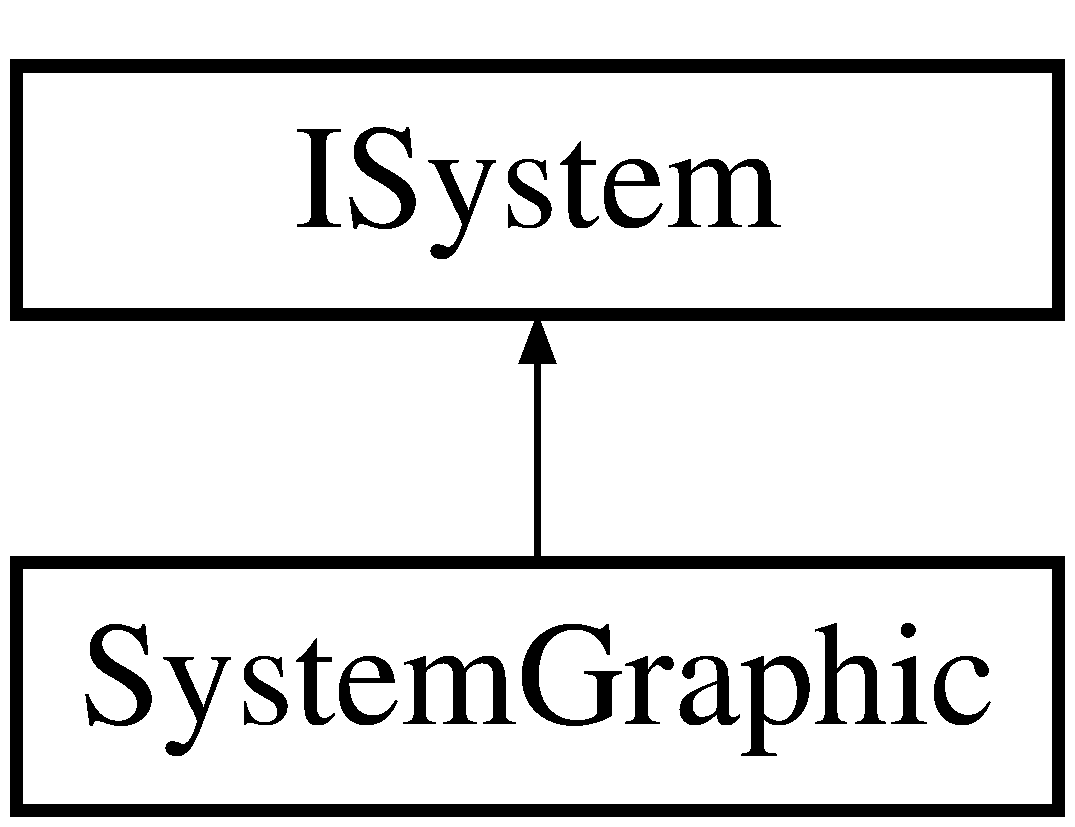
\includegraphics[height=2.000000cm]{classSystemGraphic}
\end{center}
\end{figure}
\subsection*{Métodos públicos}
\begin{DoxyCompactItemize}
\item 
\hyperlink{classSystemGraphic_a5c1878f11c82193606c51d4b10bd05f6}{System\+Graphic} (sf\+::\+Render\+Window \&window, \hyperlink{classResourceHolder}{Resource\+Holder}$<$ I\+D\+Fonts, sf\+::\+Font $>$ \&fonts, \hyperlink{classResourceHolder}{Resource\+Holder}$<$ std\+::string, sf\+::\+Texture $>$ \&images)
\item 
virtual void \hyperlink{classSystemGraphic_a792331587037bbf7fdfdd487cd45575a}{initialize} ()
\item 
virtual void \hyperlink{classSystemGraphic_af59c303890f7faf14db27ab746a23d3a}{finalize} ()
\item 
virtual void \hyperlink{classSystemGraphic_aaabd7eb4e9ce5d82dd39126239818283}{update} (sf\+::\+Time dt)
\item 
virtual void \hyperlink{classSystemGraphic_a0d46ab172987eed86b45ae016240034e}{update\+Second\+Part} (sf\+::\+Time dt)
\item 
virtual void \hyperlink{classSystemGraphic_a7b905fc340431b0521b975d82ef2fa45}{register\+Entity} (\hyperlink{classEntity}{Entity} $\ast$entity)
\item 
virtual void \hyperlink{classSystemGraphic_a9dba6a98242f2c5f07bd52301bc3dacb}{removed\+Entity} (\hyperlink{classEntity}{Entity} $\ast$entity)
\item 
\hypertarget{classSystemGraphic_a8b271e0b06df79aa780c52610042156d}{}virtual void {\bfseries execute} ()\label{classSystemGraphic_a8b271e0b06df79aa780c52610042156d}

\item 
void \hyperlink{classSystemGraphic_a926ff22280da8f657ae8b79fec5e88cd}{new\+Scene} (\hyperlink{structStructMap}{Struct\+Map} $\ast$info\+Map)
\item 
sf\+::\+Vector2f \hyperlink{classSystemGraphic_a3e38f35aebdd76068690b131c9be5904}{get\+Ratio} ()
\item 
sf\+::\+Float\+Rect \hyperlink{classSystemGraphic_a2160ae459d04c6594d824860bbda33d9}{get\+Bounds} ()
\item 
void \hyperlink{classSystemGraphic_abfc8f2497c4507fe45d4c2909bfeb6b3}{correct\+World\+Position} (sf\+::\+Vector2f position\+Center)
\item 
sf\+::\+Float\+Rect \hyperlink{classSystemGraphic_a7478ad387903d1d9cc31d4aa21aa3a8f}{get\+View\+Bounds} () const 
\item 
sf\+::\+Render\+Target \& \hyperlink{classSystemGraphic_a5b0dbf485eeaafc22d013b4a9768ebc6}{get\+Target} () const 
\item 
\hyperlink{classResourceHolder}{Resource\+Holder}$<$ I\+D\+Fonts, sf\+::\+Font $>$ \& \hyperlink{classSystemGraphic_a97463e77f261e4f733b0d7c9bcd9f56d}{get\+Fonts} () const 
\end{DoxyCompactItemize}
\subsection*{Otros miembros heredados}


\subsection{Descripción detallada}
Sistema gráfico 

\subsection{Documentación del constructor y destructor}
\hypertarget{classSystemGraphic_a5c1878f11c82193606c51d4b10bd05f6}{}\index{System\+Graphic@{System\+Graphic}!System\+Graphic@{System\+Graphic}}
\index{System\+Graphic@{System\+Graphic}!System\+Graphic@{System\+Graphic}}
\subsubsection[{System\+Graphic}]{\setlength{\rightskip}{0pt plus 5cm}System\+Graphic\+::\+System\+Graphic (
\begin{DoxyParamCaption}
\item[{sf\+::\+Render\+Window \&}]{window, }
\item[{{\bf Resource\+Holder}$<$ I\+D\+Fonts, sf\+::\+Font $>$ \&}]{fonts, }
\item[{{\bf Resource\+Holder}$<$ std\+::string, sf\+::\+Texture $>$ \&}]{images}
\end{DoxyParamCaption}
)}\label{classSystemGraphic_a5c1878f11c82193606c51d4b10bd05f6}
Constructor 
\begin{DoxyParams}{Parámetros}
{\em window} & ventana de la aplicación \\
\hline
{\em fonts} & fuentes de la aplicación \\
\hline
{\em images} & imágenes de la aplicación \\
\hline
\end{DoxyParams}


\subsection{Documentación de las funciones miembro}
\hypertarget{classSystemGraphic_abfc8f2497c4507fe45d4c2909bfeb6b3}{}\index{System\+Graphic@{System\+Graphic}!correct\+World\+Position@{correct\+World\+Position}}
\index{correct\+World\+Position@{correct\+World\+Position}!System\+Graphic@{System\+Graphic}}
\subsubsection[{correct\+World\+Position}]{\setlength{\rightskip}{0pt plus 5cm}void System\+Graphic\+::correct\+World\+Position (
\begin{DoxyParamCaption}
\item[{sf\+::\+Vector2f}]{position\+Center}
\end{DoxyParamCaption}
)}\label{classSystemGraphic_abfc8f2497c4507fe45d4c2909bfeb6b3}
C\+Orrige la posición de la cámara 
\begin{DoxyParams}{Parámetros}
{\em position\+Center} & posición en la que centrar \\
\hline
\end{DoxyParams}
\hypertarget{classSystemGraphic_af59c303890f7faf14db27ab746a23d3a}{}\index{System\+Graphic@{System\+Graphic}!finalize@{finalize}}
\index{finalize@{finalize}!System\+Graphic@{System\+Graphic}}
\subsubsection[{finalize}]{\setlength{\rightskip}{0pt plus 5cm}void System\+Graphic\+::finalize (
\begin{DoxyParamCaption}
{}
\end{DoxyParamCaption}
)\hspace{0.3cm}{\ttfamily [virtual]}}\label{classSystemGraphic_af59c303890f7faf14db27ab746a23d3a}
Finaliza el sistema 

Reimplementado de \hyperlink{classISystem_a4cc1cac06100c45d260a23d24d5618d6}{I\+System}.

\hypertarget{classSystemGraphic_a2160ae459d04c6594d824860bbda33d9}{}\index{System\+Graphic@{System\+Graphic}!get\+Bounds@{get\+Bounds}}
\index{get\+Bounds@{get\+Bounds}!System\+Graphic@{System\+Graphic}}
\subsubsection[{get\+Bounds}]{\setlength{\rightskip}{0pt plus 5cm}sf\+::\+Float\+Rect System\+Graphic\+::get\+Bounds (
\begin{DoxyParamCaption}
{}
\end{DoxyParamCaption}
)\hspace{0.3cm}{\ttfamily [inline]}}\label{classSystemGraphic_a2160ae459d04c6594d824860bbda33d9}
Devuelve los bordes del mapa \begin{DoxyReturn}{Devuelve}

\end{DoxyReturn}
\hypertarget{classSystemGraphic_a97463e77f261e4f733b0d7c9bcd9f56d}{}\index{System\+Graphic@{System\+Graphic}!get\+Fonts@{get\+Fonts}}
\index{get\+Fonts@{get\+Fonts}!System\+Graphic@{System\+Graphic}}
\subsubsection[{get\+Fonts}]{\setlength{\rightskip}{0pt plus 5cm}{\bf Resource\+Holder}$<$I\+D\+Fonts, sf\+::\+Font$>$\& System\+Graphic\+::get\+Fonts (
\begin{DoxyParamCaption}
{}
\end{DoxyParamCaption}
) const\hspace{0.3cm}{\ttfamily [inline]}}\label{classSystemGraphic_a97463e77f261e4f733b0d7c9bcd9f56d}
Devuelve las fuentes que está utilizando para dibujar \begin{DoxyReturn}{Devuelve}

\end{DoxyReturn}
\hypertarget{classSystemGraphic_a3e38f35aebdd76068690b131c9be5904}{}\index{System\+Graphic@{System\+Graphic}!get\+Ratio@{get\+Ratio}}
\index{get\+Ratio@{get\+Ratio}!System\+Graphic@{System\+Graphic}}
\subsubsection[{get\+Ratio}]{\setlength{\rightskip}{0pt plus 5cm}sf\+::\+Vector2f System\+Graphic\+::get\+Ratio (
\begin{DoxyParamCaption}
{}
\end{DoxyParamCaption}
)\hspace{0.3cm}{\ttfamily [inline]}}\label{classSystemGraphic_a3e38f35aebdd76068690b131c9be5904}
Devuelve el ratio usado para redimensionar \begin{DoxyReturn}{Devuelve}

\end{DoxyReturn}
\hypertarget{classSystemGraphic_a5b0dbf485eeaafc22d013b4a9768ebc6}{}\index{System\+Graphic@{System\+Graphic}!get\+Target@{get\+Target}}
\index{get\+Target@{get\+Target}!System\+Graphic@{System\+Graphic}}
\subsubsection[{get\+Target}]{\setlength{\rightskip}{0pt plus 5cm}sf\+::\+Render\+Target\& System\+Graphic\+::get\+Target (
\begin{DoxyParamCaption}
{}
\end{DoxyParamCaption}
) const\hspace{0.3cm}{\ttfamily [inline]}}\label{classSystemGraphic_a5b0dbf485eeaafc22d013b4a9768ebc6}
Devuelve el target en el que se dibuja \begin{DoxyReturn}{Devuelve}

\end{DoxyReturn}
\hypertarget{classSystemGraphic_a7478ad387903d1d9cc31d4aa21aa3a8f}{}\index{System\+Graphic@{System\+Graphic}!get\+View\+Bounds@{get\+View\+Bounds}}
\index{get\+View\+Bounds@{get\+View\+Bounds}!System\+Graphic@{System\+Graphic}}
\subsubsection[{get\+View\+Bounds}]{\setlength{\rightskip}{0pt plus 5cm}sf\+::\+Float\+Rect System\+Graphic\+::get\+View\+Bounds (
\begin{DoxyParamCaption}
{}
\end{DoxyParamCaption}
) const}\label{classSystemGraphic_a7478ad387903d1d9cc31d4aa21aa3a8f}
Devuelve los bordes de la vista \begin{DoxyReturn}{Devuelve}

\end{DoxyReturn}
\hypertarget{classSystemGraphic_a792331587037bbf7fdfdd487cd45575a}{}\index{System\+Graphic@{System\+Graphic}!initialize@{initialize}}
\index{initialize@{initialize}!System\+Graphic@{System\+Graphic}}
\subsubsection[{initialize}]{\setlength{\rightskip}{0pt plus 5cm}void System\+Graphic\+::initialize (
\begin{DoxyParamCaption}
{}
\end{DoxyParamCaption}
)\hspace{0.3cm}{\ttfamily [virtual]}}\label{classSystemGraphic_a792331587037bbf7fdfdd487cd45575a}
Inicializa el sistema 

Reimplementado de \hyperlink{classISystem_ac9b257acd7d03dbd7aab149792ff98af}{I\+System}.

\hypertarget{classSystemGraphic_a926ff22280da8f657ae8b79fec5e88cd}{}\index{System\+Graphic@{System\+Graphic}!new\+Scene@{new\+Scene}}
\index{new\+Scene@{new\+Scene}!System\+Graphic@{System\+Graphic}}
\subsubsection[{new\+Scene}]{\setlength{\rightskip}{0pt plus 5cm}void System\+Graphic\+::new\+Scene (
\begin{DoxyParamCaption}
\item[{{\bf Struct\+Map} $\ast$}]{info\+Map}
\end{DoxyParamCaption}
)}\label{classSystemGraphic_a926ff22280da8f657ae8b79fec5e88cd}
Crea una nueva escena gráfica 
\begin{DoxyParams}{Parámetros}
{\em info\+Map} & \\
\hline
\end{DoxyParams}
\hypertarget{classSystemGraphic_a7b905fc340431b0521b975d82ef2fa45}{}\index{System\+Graphic@{System\+Graphic}!register\+Entity@{register\+Entity}}
\index{register\+Entity@{register\+Entity}!System\+Graphic@{System\+Graphic}}
\subsubsection[{register\+Entity}]{\setlength{\rightskip}{0pt plus 5cm}void System\+Graphic\+::register\+Entity (
\begin{DoxyParamCaption}
\item[{{\bf Entity} $\ast$}]{entity}
\end{DoxyParamCaption}
)\hspace{0.3cm}{\ttfamily [virtual]}}\label{classSystemGraphic_a7b905fc340431b0521b975d82ef2fa45}
Registra una entidad en el sistema si es de su incumbencia 
\begin{DoxyParams}{Parámetros}
{\em entity} & entidad a registrar \\
\hline
\end{DoxyParams}


Implementa \hyperlink{classISystem_aaaef32b093b566b0573cb23e00f8c7ae}{I\+System}.

\hypertarget{classSystemGraphic_a9dba6a98242f2c5f07bd52301bc3dacb}{}\index{System\+Graphic@{System\+Graphic}!removed\+Entity@{removed\+Entity}}
\index{removed\+Entity@{removed\+Entity}!System\+Graphic@{System\+Graphic}}
\subsubsection[{removed\+Entity}]{\setlength{\rightskip}{0pt plus 5cm}void System\+Graphic\+::removed\+Entity (
\begin{DoxyParamCaption}
\item[{{\bf Entity} $\ast$}]{entity}
\end{DoxyParamCaption}
)\hspace{0.3cm}{\ttfamily [virtual]}}\label{classSystemGraphic_a9dba6a98242f2c5f07bd52301bc3dacb}
Elimina la entidad del sistema 
\begin{DoxyParams}{Parámetros}
{\em entity} & \\
\hline
\end{DoxyParams}


Implementa \hyperlink{classISystem_a0e966d506838cfe09543ad4ccafa4998}{I\+System}.

\hypertarget{classSystemGraphic_aaabd7eb4e9ce5d82dd39126239818283}{}\index{System\+Graphic@{System\+Graphic}!update@{update}}
\index{update@{update}!System\+Graphic@{System\+Graphic}}
\subsubsection[{update}]{\setlength{\rightskip}{0pt plus 5cm}void System\+Graphic\+::update (
\begin{DoxyParamCaption}
\item[{sf\+::\+Time}]{dt}
\end{DoxyParamCaption}
)\hspace{0.3cm}{\ttfamily [virtual]}}\label{classSystemGraphic_aaabd7eb4e9ce5d82dd39126239818283}
Actualiza el sistema en una primera tanda 
\begin{DoxyParams}{Parámetros}
{\em dt} & tiempo entre frame y frame \\
\hline
\end{DoxyParams}


Reimplementado de \hyperlink{classISystem_a6931efd2517fd0c81237beeb04297421}{I\+System}.

\hypertarget{classSystemGraphic_a0d46ab172987eed86b45ae016240034e}{}\index{System\+Graphic@{System\+Graphic}!update\+Second\+Part@{update\+Second\+Part}}
\index{update\+Second\+Part@{update\+Second\+Part}!System\+Graphic@{System\+Graphic}}
\subsubsection[{update\+Second\+Part}]{\setlength{\rightskip}{0pt plus 5cm}void System\+Graphic\+::update\+Second\+Part (
\begin{DoxyParamCaption}
\item[{sf\+::\+Time}]{dt}
\end{DoxyParamCaption}
)\hspace{0.3cm}{\ttfamily [virtual]}}\label{classSystemGraphic_a0d46ab172987eed86b45ae016240034e}
Actualiza el sistema en una segunda tanda 
\begin{DoxyParams}{Parámetros}
{\em dt} & tiempo entre frame y frame \\
\hline
\end{DoxyParams}


Reimplementado de \hyperlink{classISystem_aef2545bd6ffac18186b566e4d3d2804b}{I\+System}.



La documentación para esta clase fue generada a partir de los siguientes ficheros\+:\begin{DoxyCompactItemize}
\item 
System\+Graphic.\+h\item 
System\+Graphic.\+cpp\end{DoxyCompactItemize}

\hypertarget{classSystemManager}{}\section{Referencia de la Clase System\+Manager}
\label{classSystemManager}\index{System\+Manager@{System\+Manager}}


{\ttfamily \#include $<$System\+Manager.\+h$>$}

\subsection*{Métodos públicos}
\begin{DoxyCompactItemize}
\item 
\hypertarget{classSystemManager_a91036e83bab4d9eef28f8f125f7c13be}{}void {\bfseries add\+System} (\hyperlink{classISystem}{I\+System} $\ast$system)\label{classSystemManager_a91036e83bab4d9eef28f8f125f7c13be}

\item 
\hypertarget{classSystemManager_a17d7e8b3fe17a779b427c158d3d2acd9}{}void {\bfseries initialize\+All} ()\label{classSystemManager_a17d7e8b3fe17a779b427c158d3d2acd9}

\item 
\hypertarget{classSystemManager_a38e097df9643260dee3c06b38f183623}{}void {\bfseries finalize\+All} ()\label{classSystemManager_a38e097df9643260dee3c06b38f183623}

\item 
\hypertarget{classSystemManager_ae491338fb8d78a02d523e966a7bead76}{}void {\bfseries update\+All} (sf\+::\+Time dt)\label{classSystemManager_ae491338fb8d78a02d523e966a7bead76}

\item 
\hypertarget{classSystemManager_ad9dfb274070f5befa1980b34ca8dc9e0}{}void {\bfseries clear\+Systems} ()\label{classSystemManager_ad9dfb274070f5befa1980b34ca8dc9e0}

\item 
\hypertarget{classSystemManager_a88f8c568af7097ae892790f274bdd028}{}void {\bfseries register\+Entity} (\hyperlink{classEntity}{Entity} $\ast$entity)\label{classSystemManager_a88f8c568af7097ae892790f274bdd028}

\item 
\hypertarget{classSystemManager_aa771cc05088aaaa32dbf67863820a0c4}{}void {\bfseries remove\+Entity} (\hyperlink{classEntity}{Entity} $\ast$entity)\label{classSystemManager_aa771cc05088aaaa32dbf67863820a0c4}

\item 
\hyperlink{classISystem}{I\+System} $\ast$ \hyperlink{classSystemManager_a6c8d24328cfae009b400d32dae9d2dd7}{get\+System} (Type\+System type)
\end{DoxyCompactItemize}


\subsection{Descripción detallada}
Gestor de sistemas 

\subsection{Documentación de las funciones miembro}
\hypertarget{classSystemManager_a6c8d24328cfae009b400d32dae9d2dd7}{}\index{System\+Manager@{System\+Manager}!get\+System@{get\+System}}
\index{get\+System@{get\+System}!System\+Manager@{System\+Manager}}
\subsubsection[{get\+System}]{\setlength{\rightskip}{0pt plus 5cm}{\bf I\+System} $\ast$ System\+Manager\+::get\+System (
\begin{DoxyParamCaption}
\item[{Type\+System}]{type}
\end{DoxyParamCaption}
)}\label{classSystemManager_a6c8d24328cfae009b400d32dae9d2dd7}
Devuelve un sistema solicitado 
\begin{DoxyParams}{Parámetros}
{\em type} & tipo del sistema solicitado \\
\hline
\end{DoxyParams}
\begin{DoxyReturn}{Devuelve}
el sistema 
\end{DoxyReturn}


La documentación para esta clase fue generada a partir de los siguientes ficheros\+:\begin{DoxyCompactItemize}
\item 
System\+Manager.\+h\item 
System\+Manager.\+cpp\end{DoxyCompactItemize}

\hypertarget{classSystemMovement}{}\section{Referencia de la Clase System\+Movement}
\label{classSystemMovement}\index{System\+Movement@{System\+Movement}}


{\ttfamily \#include $<$System\+Movement.\+h$>$}

Diagrama de herencias de System\+Movement\begin{figure}[H]
\begin{center}
\leavevmode
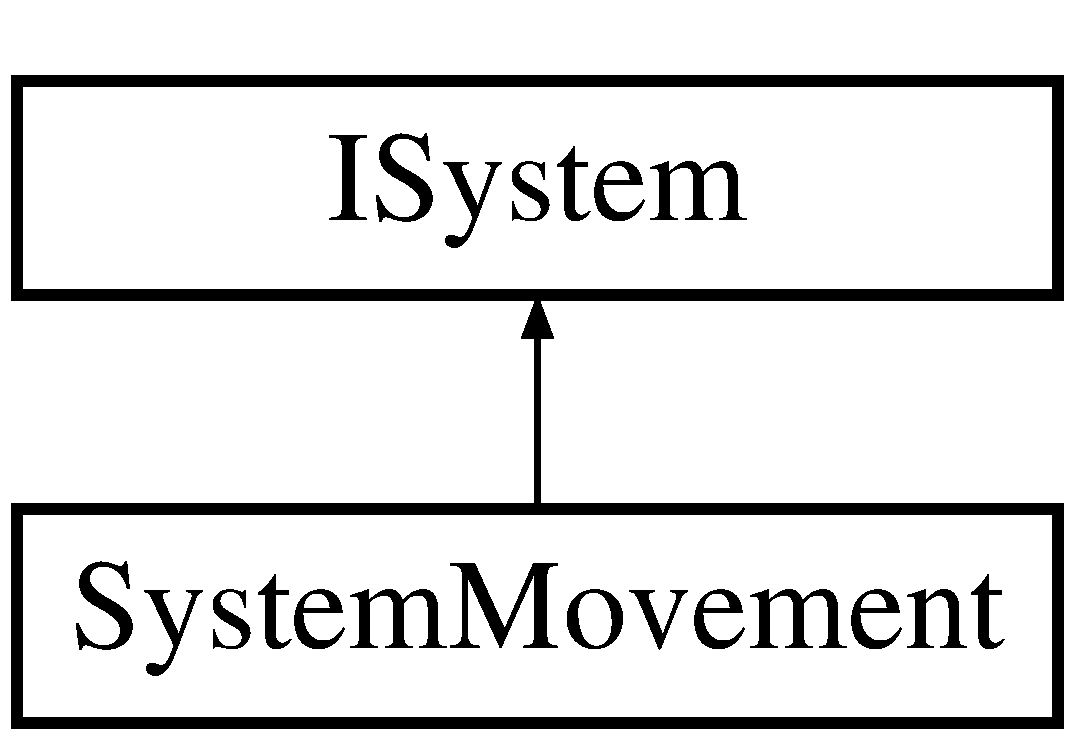
\includegraphics[height=2.000000cm]{classSystemMovement}
\end{center}
\end{figure}
\subsection*{Métodos públicos}
\begin{DoxyCompactItemize}
\item 
virtual void \hyperlink{classSystemMovement_a5657b5507fd4f6a7bf92e9a9929881d3}{initialize} ()
\item 
virtual void \hyperlink{classSystemMovement_a2e4df7be9f17a4572116649552c9d073}{finalize} ()
\item 
virtual void \hyperlink{classSystemMovement_aab4a789b0bf9d329461896e12ada82c4}{update} (sf\+::\+Time dt)
\item 
virtual void \hyperlink{classSystemMovement_afd66e76ecd00084594be9334434a689d}{update\+Second\+Part} (sf\+::\+Time dt)
\item 
virtual void \hyperlink{classSystemMovement_ae7a01c74fcd8cfae49488a707cf32902}{register\+Entity} (\hyperlink{classEntity}{Entity} $\ast$entity)
\item 
virtual void \hyperlink{classSystemMovement_a7fe2e159ce9ef32f5710d9a957a2450b}{removed\+Entity} (\hyperlink{classEntity}{Entity} $\ast$entity)
\end{DoxyCompactItemize}
\subsection*{Otros miembros heredados}


\subsection{Descripción detallada}
Sistema de movimiento 

\subsection{Documentación de las funciones miembro}
\hypertarget{classSystemMovement_a2e4df7be9f17a4572116649552c9d073}{}\index{System\+Movement@{System\+Movement}!finalize@{finalize}}
\index{finalize@{finalize}!System\+Movement@{System\+Movement}}
\subsubsection[{finalize}]{\setlength{\rightskip}{0pt plus 5cm}void System\+Movement\+::finalize (
\begin{DoxyParamCaption}
{}
\end{DoxyParamCaption}
)\hspace{0.3cm}{\ttfamily [virtual]}}\label{classSystemMovement_a2e4df7be9f17a4572116649552c9d073}
Finaliza el sistema 

Reimplementado de \hyperlink{classISystem_a4cc1cac06100c45d260a23d24d5618d6}{I\+System}.

\hypertarget{classSystemMovement_a5657b5507fd4f6a7bf92e9a9929881d3}{}\index{System\+Movement@{System\+Movement}!initialize@{initialize}}
\index{initialize@{initialize}!System\+Movement@{System\+Movement}}
\subsubsection[{initialize}]{\setlength{\rightskip}{0pt plus 5cm}void System\+Movement\+::initialize (
\begin{DoxyParamCaption}
{}
\end{DoxyParamCaption}
)\hspace{0.3cm}{\ttfamily [virtual]}}\label{classSystemMovement_a5657b5507fd4f6a7bf92e9a9929881d3}
Inicializa el sistema 

Reimplementado de \hyperlink{classISystem_ac9b257acd7d03dbd7aab149792ff98af}{I\+System}.

\hypertarget{classSystemMovement_ae7a01c74fcd8cfae49488a707cf32902}{}\index{System\+Movement@{System\+Movement}!register\+Entity@{register\+Entity}}
\index{register\+Entity@{register\+Entity}!System\+Movement@{System\+Movement}}
\subsubsection[{register\+Entity}]{\setlength{\rightskip}{0pt plus 5cm}void System\+Movement\+::register\+Entity (
\begin{DoxyParamCaption}
\item[{{\bf Entity} $\ast$}]{entity}
\end{DoxyParamCaption}
)\hspace{0.3cm}{\ttfamily [virtual]}}\label{classSystemMovement_ae7a01c74fcd8cfae49488a707cf32902}
Registra una entidad en el sistema si es de su incumbencia 
\begin{DoxyParams}{Parámetros}
{\em entity} & entidad a registrar \\
\hline
\end{DoxyParams}


Implementa \hyperlink{classISystem_aaaef32b093b566b0573cb23e00f8c7ae}{I\+System}.

\hypertarget{classSystemMovement_a7fe2e159ce9ef32f5710d9a957a2450b}{}\index{System\+Movement@{System\+Movement}!removed\+Entity@{removed\+Entity}}
\index{removed\+Entity@{removed\+Entity}!System\+Movement@{System\+Movement}}
\subsubsection[{removed\+Entity}]{\setlength{\rightskip}{0pt plus 5cm}void System\+Movement\+::removed\+Entity (
\begin{DoxyParamCaption}
\item[{{\bf Entity} $\ast$}]{entity}
\end{DoxyParamCaption}
)\hspace{0.3cm}{\ttfamily [virtual]}}\label{classSystemMovement_a7fe2e159ce9ef32f5710d9a957a2450b}
Elimina la entidad del sistema 
\begin{DoxyParams}{Parámetros}
{\em entity} & \\
\hline
\end{DoxyParams}


Implementa \hyperlink{classISystem_a0e966d506838cfe09543ad4ccafa4998}{I\+System}.

\hypertarget{classSystemMovement_aab4a789b0bf9d329461896e12ada82c4}{}\index{System\+Movement@{System\+Movement}!update@{update}}
\index{update@{update}!System\+Movement@{System\+Movement}}
\subsubsection[{update}]{\setlength{\rightskip}{0pt plus 5cm}void System\+Movement\+::update (
\begin{DoxyParamCaption}
\item[{sf\+::\+Time}]{dt}
\end{DoxyParamCaption}
)\hspace{0.3cm}{\ttfamily [virtual]}}\label{classSystemMovement_aab4a789b0bf9d329461896e12ada82c4}
Actualiza el sistema en una primera tanda 
\begin{DoxyParams}{Parámetros}
{\em dt} & tiempo entre frame y frame \\
\hline
\end{DoxyParams}


Reimplementado de \hyperlink{classISystem_a6931efd2517fd0c81237beeb04297421}{I\+System}.

\hypertarget{classSystemMovement_afd66e76ecd00084594be9334434a689d}{}\index{System\+Movement@{System\+Movement}!update\+Second\+Part@{update\+Second\+Part}}
\index{update\+Second\+Part@{update\+Second\+Part}!System\+Movement@{System\+Movement}}
\subsubsection[{update\+Second\+Part}]{\setlength{\rightskip}{0pt plus 5cm}void System\+Movement\+::update\+Second\+Part (
\begin{DoxyParamCaption}
\item[{sf\+::\+Time}]{dt}
\end{DoxyParamCaption}
)\hspace{0.3cm}{\ttfamily [virtual]}}\label{classSystemMovement_afd66e76ecd00084594be9334434a689d}
Actualiza el sistema en una segunda tanda 
\begin{DoxyParams}{Parámetros}
{\em dt} & tiempo entre frame y frame \\
\hline
\end{DoxyParams}


Reimplementado de \hyperlink{classISystem_aef2545bd6ffac18186b566e4d3d2804b}{I\+System}.



La documentación para esta clase fue generada a partir de los siguientes ficheros\+:\begin{DoxyCompactItemize}
\item 
System\+Movement.\+h\item 
System\+Movement.\+cpp\end{DoxyCompactItemize}

\hypertarget{classSystemObjectsGame}{}\section{Referencia de la Clase System\+Objects\+Game}
\label{classSystemObjectsGame}\index{System\+Objects\+Game@{System\+Objects\+Game}}


{\ttfamily \#include $<$System\+Objects\+Game.\+h$>$}

Diagrama de herencias de System\+Objects\+Game\begin{figure}[H]
\begin{center}
\leavevmode
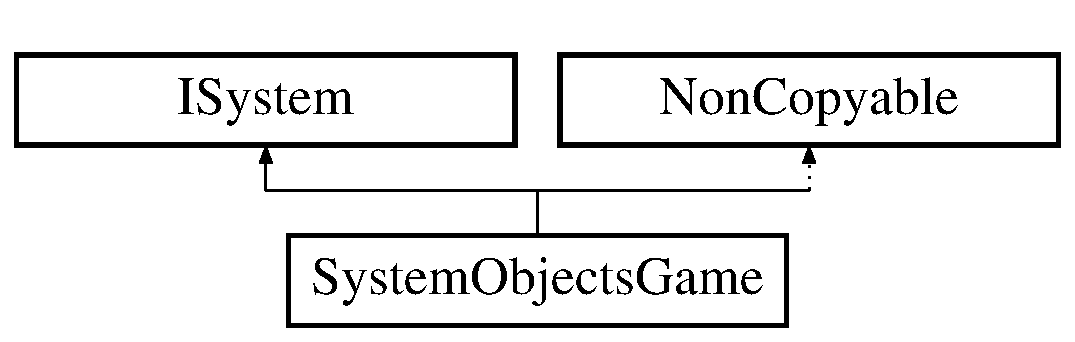
\includegraphics[height=2.000000cm]{classSystemObjectsGame}
\end{center}
\end{figure}
\subsection*{Métodos públicos}
\begin{DoxyCompactItemize}
\item 
\hyperlink{classSystemObjectsGame_a8f9dff3f4bc88ebbd64094241448633c}{System\+Objects\+Game} (\hyperlink{classSystemManager}{System\+Manager} \&system\+Manager)
\item 
virtual \hyperlink{classSystemObjectsGame_ae32e62e6afe1c353a8c888d15324f01e}{$\sim$\+System\+Objects\+Game} ()
\item 
virtual void \hyperlink{classSystemObjectsGame_a1d915c3471432c344a58af523085b87f}{initialize} ()
\item 
virtual void \hyperlink{classSystemObjectsGame_a4357e0e5d2e42a6b3e80362cbfdbda39}{finalize} ()
\item 
virtual void \hyperlink{classSystemObjectsGame_a6d8cbcab3b14a4ddc4c45ebe0c7aed07}{register\+Entity} (\hyperlink{classEntity}{Entity} $\ast$entity)
\item 
virtual void \hyperlink{classSystemObjectsGame_ae716ba020dded37eb7cc01e3dab32a1a}{removed\+Entity} (\hyperlink{classEntity}{Entity} $\ast$entity)
\item 
virtual void \hyperlink{classSystemObjectsGame_a6836f71bd70b620d8b86b98e6e3ee44b}{update} (sf\+::\+Time dt)
\item 
virtual void \hyperlink{classSystemObjectsGame_ad238ad4e70fb3cc2a5648a7176e69233}{update\+Second\+Part} (sf\+::\+Time dt)
\item 
\hyperlink{classSubject}{Subject} $\ast$ \hyperlink{classSystemObjectsGame_a7d1bed32c2cb7ffc4731c21491668e6b}{get\+Message\+Entities} () const 
\item 
\hyperlink{classEntity}{Entity} $\ast$ \hyperlink{classSystemObjectsGame_a27f5cdf50a6091f3b44bf5232f30455d}{get\+Entity} (\hyperlink{classIdEntity}{Id\+Entity} id)
\item 
\hyperlink{classEntity}{Entity} $\ast$ \hyperlink{classSystemObjectsGame_ae8adeb2489ef7e3f8bde37d1c7cb4653}{get\+Entity\+Xml} (\hyperlink{classIdEntity}{Id\+Entity} id)
\item 
void \hyperlink{classSystemObjectsGame_a86d70dfc35a07455330789de8503b153}{destroy\+Entity} (\hyperlink{classIdEntity}{Id\+Entity} id)
\end{DoxyCompactItemize}
\subsection*{Otros miembros heredados}


\subsection{Descripción detallada}
Sistema de entidades del juego 

\subsection{Documentación del constructor y destructor}
\hypertarget{classSystemObjectsGame_a8f9dff3f4bc88ebbd64094241448633c}{}\index{System\+Objects\+Game@{System\+Objects\+Game}!System\+Objects\+Game@{System\+Objects\+Game}}
\index{System\+Objects\+Game@{System\+Objects\+Game}!System\+Objects\+Game@{System\+Objects\+Game}}
\subsubsection[{System\+Objects\+Game}]{\setlength{\rightskip}{0pt plus 5cm}System\+Objects\+Game\+::\+System\+Objects\+Game (
\begin{DoxyParamCaption}
\item[{{\bf System\+Manager} \&}]{system\+Manager}
\end{DoxyParamCaption}
)}\label{classSystemObjectsGame_a8f9dff3f4bc88ebbd64094241448633c}
Constructor 
\begin{DoxyParams}{Parámetros}
{\em system\+Manager} & gestor de sistemas \\
\hline
\end{DoxyParams}
\hypertarget{classSystemObjectsGame_ae32e62e6afe1c353a8c888d15324f01e}{}\index{System\+Objects\+Game@{System\+Objects\+Game}!````~System\+Objects\+Game@{$\sim$\+System\+Objects\+Game}}
\index{````~System\+Objects\+Game@{$\sim$\+System\+Objects\+Game}!System\+Objects\+Game@{System\+Objects\+Game}}
\subsubsection[{$\sim$\+System\+Objects\+Game}]{\setlength{\rightskip}{0pt plus 5cm}System\+Objects\+Game\+::$\sim$\+System\+Objects\+Game (
\begin{DoxyParamCaption}
{}
\end{DoxyParamCaption}
)\hspace{0.3cm}{\ttfamily [virtual]}}\label{classSystemObjectsGame_ae32e62e6afe1c353a8c888d15324f01e}
Destructor 

\subsection{Documentación de las funciones miembro}
\hypertarget{classSystemObjectsGame_a86d70dfc35a07455330789de8503b153}{}\index{System\+Objects\+Game@{System\+Objects\+Game}!destroy\+Entity@{destroy\+Entity}}
\index{destroy\+Entity@{destroy\+Entity}!System\+Objects\+Game@{System\+Objects\+Game}}
\subsubsection[{destroy\+Entity}]{\setlength{\rightskip}{0pt plus 5cm}void System\+Objects\+Game\+::destroy\+Entity (
\begin{DoxyParamCaption}
\item[{{\bf Id\+Entity}}]{id}
\end{DoxyParamCaption}
)}\label{classSystemObjectsGame_a86d70dfc35a07455330789de8503b153}
Borra una entidad 
\begin{DoxyParams}{Parámetros}
{\em id} & identificador de la entidad \\
\hline
\end{DoxyParams}
\hypertarget{classSystemObjectsGame_a4357e0e5d2e42a6b3e80362cbfdbda39}{}\index{System\+Objects\+Game@{System\+Objects\+Game}!finalize@{finalize}}
\index{finalize@{finalize}!System\+Objects\+Game@{System\+Objects\+Game}}
\subsubsection[{finalize}]{\setlength{\rightskip}{0pt plus 5cm}void System\+Objects\+Game\+::finalize (
\begin{DoxyParamCaption}
{}
\end{DoxyParamCaption}
)\hspace{0.3cm}{\ttfamily [virtual]}}\label{classSystemObjectsGame_a4357e0e5d2e42a6b3e80362cbfdbda39}
Finaliza el sistema 

Reimplementado de \hyperlink{classISystem_a4cc1cac06100c45d260a23d24d5618d6}{I\+System}.

\hypertarget{classSystemObjectsGame_a27f5cdf50a6091f3b44bf5232f30455d}{}\index{System\+Objects\+Game@{System\+Objects\+Game}!get\+Entity@{get\+Entity}}
\index{get\+Entity@{get\+Entity}!System\+Objects\+Game@{System\+Objects\+Game}}
\subsubsection[{get\+Entity}]{\setlength{\rightskip}{0pt plus 5cm}{\bf Entity} $\ast$ System\+Objects\+Game\+::get\+Entity (
\begin{DoxyParamCaption}
\item[{{\bf Id\+Entity}}]{id}
\end{DoxyParamCaption}
)}\label{classSystemObjectsGame_a27f5cdf50a6091f3b44bf5232f30455d}
Devuelve la entidad solicitada 
\begin{DoxyParams}{Parámetros}
{\em id} & identificador de la entidad solicitada \\
\hline
\end{DoxyParams}
\begin{DoxyReturn}{Devuelve}
la entidad solicitada, si no lo encuentra, salta excepción 
\end{DoxyReturn}
\hypertarget{classSystemObjectsGame_ae8adeb2489ef7e3f8bde37d1c7cb4653}{}\index{System\+Objects\+Game@{System\+Objects\+Game}!get\+Entity\+Xml@{get\+Entity\+Xml}}
\index{get\+Entity\+Xml@{get\+Entity\+Xml}!System\+Objects\+Game@{System\+Objects\+Game}}
\subsubsection[{get\+Entity\+Xml}]{\setlength{\rightskip}{0pt plus 5cm}{\bf Entity} $\ast$ System\+Objects\+Game\+::get\+Entity\+Xml (
\begin{DoxyParamCaption}
\item[{{\bf Id\+Entity}}]{id}
\end{DoxyParamCaption}
)}\label{classSystemObjectsGame_ae8adeb2489ef7e3f8bde37d1c7cb4653}
Devuelve la entidad solicitada 
\begin{DoxyParams}{Parámetros}
{\em id} & identificador del xml de la entidad solicitada \\
\hline
\end{DoxyParams}
\begin{DoxyReturn}{Devuelve}
la entidad solicitada, si no lo encuentra, salta excepción 
\end{DoxyReturn}
\hypertarget{classSystemObjectsGame_a7d1bed32c2cb7ffc4731c21491668e6b}{}\index{System\+Objects\+Game@{System\+Objects\+Game}!get\+Message\+Entities@{get\+Message\+Entities}}
\index{get\+Message\+Entities@{get\+Message\+Entities}!System\+Objects\+Game@{System\+Objects\+Game}}
\subsubsection[{get\+Message\+Entities}]{\setlength{\rightskip}{0pt plus 5cm}{\bf Subject}$\ast$ System\+Objects\+Game\+::get\+Message\+Entities (
\begin{DoxyParamCaption}
{}
\end{DoxyParamCaption}
) const\hspace{0.3cm}{\ttfamily [inline]}}\label{classSystemObjectsGame_a7d1bed32c2cb7ffc4731c21491668e6b}
Devuelve el objeto vigilado del patrón observer \begin{DoxyReturn}{Devuelve}

\end{DoxyReturn}
\hypertarget{classSystemObjectsGame_a1d915c3471432c344a58af523085b87f}{}\index{System\+Objects\+Game@{System\+Objects\+Game}!initialize@{initialize}}
\index{initialize@{initialize}!System\+Objects\+Game@{System\+Objects\+Game}}
\subsubsection[{initialize}]{\setlength{\rightskip}{0pt plus 5cm}void System\+Objects\+Game\+::initialize (
\begin{DoxyParamCaption}
{}
\end{DoxyParamCaption}
)\hspace{0.3cm}{\ttfamily [virtual]}}\label{classSystemObjectsGame_a1d915c3471432c344a58af523085b87f}
Inicializa el sistema 

Reimplementado de \hyperlink{classISystem_ac9b257acd7d03dbd7aab149792ff98af}{I\+System}.

\hypertarget{classSystemObjectsGame_a6d8cbcab3b14a4ddc4c45ebe0c7aed07}{}\index{System\+Objects\+Game@{System\+Objects\+Game}!register\+Entity@{register\+Entity}}
\index{register\+Entity@{register\+Entity}!System\+Objects\+Game@{System\+Objects\+Game}}
\subsubsection[{register\+Entity}]{\setlength{\rightskip}{0pt plus 5cm}void System\+Objects\+Game\+::register\+Entity (
\begin{DoxyParamCaption}
\item[{{\bf Entity} $\ast$}]{entity}
\end{DoxyParamCaption}
)\hspace{0.3cm}{\ttfamily [virtual]}}\label{classSystemObjectsGame_a6d8cbcab3b14a4ddc4c45ebe0c7aed07}
Registra una entidad en el sistema si es de su incumbencia 
\begin{DoxyParams}{Parámetros}
{\em entity} & entidad a registrar \\
\hline
\end{DoxyParams}


Implementa \hyperlink{classISystem_aaaef32b093b566b0573cb23e00f8c7ae}{I\+System}.

\hypertarget{classSystemObjectsGame_ae716ba020dded37eb7cc01e3dab32a1a}{}\index{System\+Objects\+Game@{System\+Objects\+Game}!removed\+Entity@{removed\+Entity}}
\index{removed\+Entity@{removed\+Entity}!System\+Objects\+Game@{System\+Objects\+Game}}
\subsubsection[{removed\+Entity}]{\setlength{\rightskip}{0pt plus 5cm}virtual void System\+Objects\+Game\+::removed\+Entity (
\begin{DoxyParamCaption}
\item[{{\bf Entity} $\ast$}]{entity}
\end{DoxyParamCaption}
)\hspace{0.3cm}{\ttfamily [inline]}, {\ttfamily [virtual]}}\label{classSystemObjectsGame_ae716ba020dded37eb7cc01e3dab32a1a}
Elimina la entidad del sistema 
\begin{DoxyParams}{Parámetros}
{\em entity} & \\
\hline
\end{DoxyParams}


Implementa \hyperlink{classISystem_a0e966d506838cfe09543ad4ccafa4998}{I\+System}.

\hypertarget{classSystemObjectsGame_a6836f71bd70b620d8b86b98e6e3ee44b}{}\index{System\+Objects\+Game@{System\+Objects\+Game}!update@{update}}
\index{update@{update}!System\+Objects\+Game@{System\+Objects\+Game}}
\subsubsection[{update}]{\setlength{\rightskip}{0pt plus 5cm}void System\+Objects\+Game\+::update (
\begin{DoxyParamCaption}
\item[{sf\+::\+Time}]{dt}
\end{DoxyParamCaption}
)\hspace{0.3cm}{\ttfamily [virtual]}}\label{classSystemObjectsGame_a6836f71bd70b620d8b86b98e6e3ee44b}
Actualiza el sistema en una primera tanda 
\begin{DoxyParams}{Parámetros}
{\em dt} & tiempo entre frame y frame \\
\hline
\end{DoxyParams}


Reimplementado de \hyperlink{classISystem_a6931efd2517fd0c81237beeb04297421}{I\+System}.

\hypertarget{classSystemObjectsGame_ad238ad4e70fb3cc2a5648a7176e69233}{}\index{System\+Objects\+Game@{System\+Objects\+Game}!update\+Second\+Part@{update\+Second\+Part}}
\index{update\+Second\+Part@{update\+Second\+Part}!System\+Objects\+Game@{System\+Objects\+Game}}
\subsubsection[{update\+Second\+Part}]{\setlength{\rightskip}{0pt plus 5cm}virtual void System\+Objects\+Game\+::update\+Second\+Part (
\begin{DoxyParamCaption}
\item[{sf\+::\+Time}]{dt}
\end{DoxyParamCaption}
)\hspace{0.3cm}{\ttfamily [inline]}, {\ttfamily [virtual]}}\label{classSystemObjectsGame_ad238ad4e70fb3cc2a5648a7176e69233}
Actualiza el sistema en una segunda tanda 
\begin{DoxyParams}{Parámetros}
{\em dt} & tiempo entre frame y frame \\
\hline
\end{DoxyParams}


Reimplementado de \hyperlink{classISystem_aef2545bd6ffac18186b566e4d3d2804b}{I\+System}.



La documentación para esta clase fue generada a partir de los siguientes ficheros\+:\begin{DoxyCompactItemize}
\item 
System\+Objects\+Game.\+h\item 
System\+Objects\+Game.\+cpp\end{DoxyCompactItemize}

\hypertarget{classSystemQuest}{}\section{Referencia de la Clase System\+Quest}
\label{classSystemQuest}\index{System\+Quest@{System\+Quest}}


{\ttfamily \#include $<$System\+Quest.\+h$>$}

Diagrama de herencias de System\+Quest\begin{figure}[H]
\begin{center}
\leavevmode
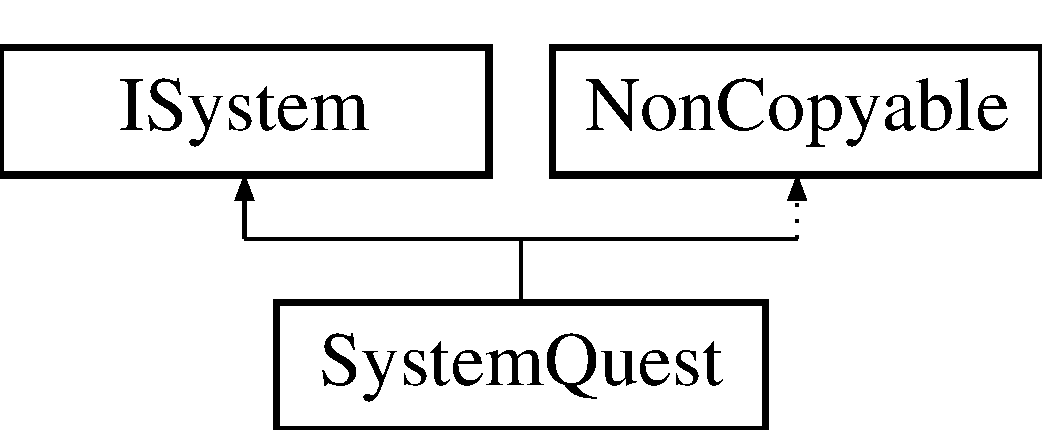
\includegraphics[height=2.000000cm]{classSystemQuest}
\end{center}
\end{figure}
\subsection*{Métodos públicos}
\begin{DoxyCompactItemize}
\item 
virtual void \hyperlink{classSystemQuest_a48773430521559d0b5eaa931b53d8892}{initialize} ()
\item 
virtual void \hyperlink{classSystemQuest_a3c9f834570acf2277d4620e3ba16992d}{finalize} ()
\item 
virtual void \hyperlink{classSystemQuest_a03ce5db7875898ebae8c9424c1888c37}{register\+Entity} (\hyperlink{classEntity}{Entity} $\ast$entity)
\item 
virtual void \hyperlink{classSystemQuest_a588e9982c16288af4675b67bf9177080}{removed\+Entity} (\hyperlink{classEntity}{Entity} $\ast$entity)
\item 
virtual void \hyperlink{classSystemQuest_a76892fc5b11bdb7132e7499e46eb7977}{update} (sf\+::\+Time dt)
\item 
virtual void \hyperlink{classSystemQuest_a3069bdc81a590c47c4479b63add3fc3d}{update\+Second\+Part} (sf\+::\+Time dt)
\item 
Mission\+Status \hyperlink{classSystemQuest_a6469f12a86c708f7661482aad85b1de7}{get\+Status} ()
\item 
void \hyperlink{classSystemQuest_aca9a6f845d267fc9ef58d6531b341094}{add\+Quest} (\hyperlink{classQuest}{Quest} $\ast$quest)
\item 
sf\+::\+String $\ast$ \hyperlink{classSystemQuest_a3c5b341ae4087af5b1a0a0386905bfd7}{to\+String} ()
\end{DoxyCompactItemize}
\subsection*{Otros miembros heredados}


\subsection{Descripción detallada}
Sistema de misiones 

\subsection{Documentación de las funciones miembro}
\hypertarget{classSystemQuest_aca9a6f845d267fc9ef58d6531b341094}{}\index{System\+Quest@{System\+Quest}!add\+Quest@{add\+Quest}}
\index{add\+Quest@{add\+Quest}!System\+Quest@{System\+Quest}}
\subsubsection[{add\+Quest}]{\setlength{\rightskip}{0pt plus 5cm}void System\+Quest\+::add\+Quest (
\begin{DoxyParamCaption}
\item[{{\bf Quest} $\ast$}]{quest}
\end{DoxyParamCaption}
)}\label{classSystemQuest_aca9a6f845d267fc9ef58d6531b341094}
Añade una nueva misión al sistema 
\begin{DoxyParams}{Parámetros}
{\em quest} & \\
\hline
\end{DoxyParams}
\hypertarget{classSystemQuest_a3c9f834570acf2277d4620e3ba16992d}{}\index{System\+Quest@{System\+Quest}!finalize@{finalize}}
\index{finalize@{finalize}!System\+Quest@{System\+Quest}}
\subsubsection[{finalize}]{\setlength{\rightskip}{0pt plus 5cm}void System\+Quest\+::finalize (
\begin{DoxyParamCaption}
{}
\end{DoxyParamCaption}
)\hspace{0.3cm}{\ttfamily [virtual]}}\label{classSystemQuest_a3c9f834570acf2277d4620e3ba16992d}
Finaliza el sistema 

Reimplementado de \hyperlink{classISystem_a4cc1cac06100c45d260a23d24d5618d6}{I\+System}.

\hypertarget{classSystemQuest_a6469f12a86c708f7661482aad85b1de7}{}\index{System\+Quest@{System\+Quest}!get\+Status@{get\+Status}}
\index{get\+Status@{get\+Status}!System\+Quest@{System\+Quest}}
\subsubsection[{get\+Status}]{\setlength{\rightskip}{0pt plus 5cm}Mission\+Status System\+Quest\+::get\+Status (
\begin{DoxyParamCaption}
{}
\end{DoxyParamCaption}
)}\label{classSystemQuest_a6469f12a86c708f7661482aad85b1de7}
Devuelve el estado de las misiones, de forma que se sepa si ha ganado o perdido el juego, o está en marcha todavía \begin{DoxyReturn}{Devuelve}
estado del juego 
\end{DoxyReturn}
\hypertarget{classSystemQuest_a48773430521559d0b5eaa931b53d8892}{}\index{System\+Quest@{System\+Quest}!initialize@{initialize}}
\index{initialize@{initialize}!System\+Quest@{System\+Quest}}
\subsubsection[{initialize}]{\setlength{\rightskip}{0pt plus 5cm}void System\+Quest\+::initialize (
\begin{DoxyParamCaption}
{}
\end{DoxyParamCaption}
)\hspace{0.3cm}{\ttfamily [virtual]}}\label{classSystemQuest_a48773430521559d0b5eaa931b53d8892}
Inicializa el sistema 

Reimplementado de \hyperlink{classISystem_ac9b257acd7d03dbd7aab149792ff98af}{I\+System}.

\hypertarget{classSystemQuest_a03ce5db7875898ebae8c9424c1888c37}{}\index{System\+Quest@{System\+Quest}!register\+Entity@{register\+Entity}}
\index{register\+Entity@{register\+Entity}!System\+Quest@{System\+Quest}}
\subsubsection[{register\+Entity}]{\setlength{\rightskip}{0pt plus 5cm}void System\+Quest\+::register\+Entity (
\begin{DoxyParamCaption}
\item[{{\bf Entity} $\ast$}]{entity}
\end{DoxyParamCaption}
)\hspace{0.3cm}{\ttfamily [virtual]}}\label{classSystemQuest_a03ce5db7875898ebae8c9424c1888c37}
Registra una entidad en el sistema si es de su incumbencia 
\begin{DoxyParams}{Parámetros}
{\em entity} & entidad a registrar \\
\hline
\end{DoxyParams}


Implementa \hyperlink{classISystem_aaaef32b093b566b0573cb23e00f8c7ae}{I\+System}.

\hypertarget{classSystemQuest_a588e9982c16288af4675b67bf9177080}{}\index{System\+Quest@{System\+Quest}!removed\+Entity@{removed\+Entity}}
\index{removed\+Entity@{removed\+Entity}!System\+Quest@{System\+Quest}}
\subsubsection[{removed\+Entity}]{\setlength{\rightskip}{0pt plus 5cm}void System\+Quest\+::removed\+Entity (
\begin{DoxyParamCaption}
\item[{{\bf Entity} $\ast$}]{entity}
\end{DoxyParamCaption}
)\hspace{0.3cm}{\ttfamily [virtual]}}\label{classSystemQuest_a588e9982c16288af4675b67bf9177080}
Elimina la entidad del sistema 
\begin{DoxyParams}{Parámetros}
{\em entity} & \\
\hline
\end{DoxyParams}


Implementa \hyperlink{classISystem_a0e966d506838cfe09543ad4ccafa4998}{I\+System}.

\hypertarget{classSystemQuest_a3c5b341ae4087af5b1a0a0386905bfd7}{}\index{System\+Quest@{System\+Quest}!to\+String@{to\+String}}
\index{to\+String@{to\+String}!System\+Quest@{System\+Quest}}
\subsubsection[{to\+String}]{\setlength{\rightskip}{0pt plus 5cm}sf\+::\+String $\ast$ System\+Quest\+::to\+String (
\begin{DoxyParamCaption}
{}
\end{DoxyParamCaption}
)}\label{classSystemQuest_a3c5b341ae4087af5b1a0a0386905bfd7}
Devuelve un string representando las missiones y si están completas \begin{DoxyReturn}{Devuelve}

\end{DoxyReturn}
\hypertarget{classSystemQuest_a76892fc5b11bdb7132e7499e46eb7977}{}\index{System\+Quest@{System\+Quest}!update@{update}}
\index{update@{update}!System\+Quest@{System\+Quest}}
\subsubsection[{update}]{\setlength{\rightskip}{0pt plus 5cm}void System\+Quest\+::update (
\begin{DoxyParamCaption}
\item[{sf\+::\+Time}]{dt}
\end{DoxyParamCaption}
)\hspace{0.3cm}{\ttfamily [virtual]}}\label{classSystemQuest_a76892fc5b11bdb7132e7499e46eb7977}
Actualiza el sistema en una primera tanda 
\begin{DoxyParams}{Parámetros}
{\em dt} & tiempo entre frame y frame \\
\hline
\end{DoxyParams}


Reimplementado de \hyperlink{classISystem_a6931efd2517fd0c81237beeb04297421}{I\+System}.

\hypertarget{classSystemQuest_a3069bdc81a590c47c4479b63add3fc3d}{}\index{System\+Quest@{System\+Quest}!update\+Second\+Part@{update\+Second\+Part}}
\index{update\+Second\+Part@{update\+Second\+Part}!System\+Quest@{System\+Quest}}
\subsubsection[{update\+Second\+Part}]{\setlength{\rightskip}{0pt plus 5cm}virtual void System\+Quest\+::update\+Second\+Part (
\begin{DoxyParamCaption}
\item[{sf\+::\+Time}]{dt}
\end{DoxyParamCaption}
)\hspace{0.3cm}{\ttfamily [inline]}, {\ttfamily [virtual]}}\label{classSystemQuest_a3069bdc81a590c47c4479b63add3fc3d}
Actualiza el sistema en una segunda tanda 
\begin{DoxyParams}{Parámetros}
{\em dt} & tiempo entre frame y frame \\
\hline
\end{DoxyParams}


Reimplementado de \hyperlink{classISystem_aef2545bd6ffac18186b566e4d3d2804b}{I\+System}.



La documentación para esta clase fue generada a partir de los siguientes ficheros\+:\begin{DoxyCompactItemize}
\item 
System\+Quest.\+h\item 
System\+Quest.\+cpp\end{DoxyCompactItemize}

\hypertarget{structTalk}{}\section{Referencia de la Estructura Talk}
\label{structTalk}\index{Talk@{Talk}}


{\ttfamily \#include $<$Talk.\+h$>$}

\subsection*{Métodos públicos}
\begin{DoxyCompactItemize}
\item 
\hyperlink{structTalk_a9f4d707d51e7567f729116a030121560}{Talk} (sf\+::\+String $\ast$phrase)
\end{DoxyCompactItemize}
\subsection*{Campos de datos}
\begin{DoxyCompactItemize}
\item 
\hypertarget{structTalk_a01cc740b3b227031c297e7ea8afed027}{}sf\+::\+String $\ast$ {\bfseries phrase}\label{structTalk_a01cc740b3b227031c297e7ea8afed027}

\end{DoxyCompactItemize}


\subsection{Descripción detallada}
Estructura para guardar una conversación 

\subsection{Documentación del constructor y destructor}
\hypertarget{structTalk_a9f4d707d51e7567f729116a030121560}{}\index{Talk@{Talk}!Talk@{Talk}}
\index{Talk@{Talk}!Talk@{Talk}}
\subsubsection[{Talk}]{\setlength{\rightskip}{0pt plus 5cm}Talk\+::\+Talk (
\begin{DoxyParamCaption}
\item[{sf\+::\+String $\ast$}]{phrase}
\end{DoxyParamCaption}
)\hspace{0.3cm}{\ttfamily [inline]}}\label{structTalk_a9f4d707d51e7567f729116a030121560}
Constructor 
\begin{DoxyParams}{Parámetros}
{\em phrase} & frase a decir \\
\hline
\end{DoxyParams}


La documentación para esta estructura fue generada a partir del siguiente fichero\+:\begin{DoxyCompactItemize}
\item 
Talk.\+h\end{DoxyCompactItemize}

\hypertarget{classTextNode}{}\section{Referencia de la Clase Text\+Node}
\label{classTextNode}\index{Text\+Node@{Text\+Node}}


{\ttfamily \#include $<$Text\+Node.\+h$>$}

Diagrama de herencias de Text\+Node\begin{figure}[H]
\begin{center}
\leavevmode
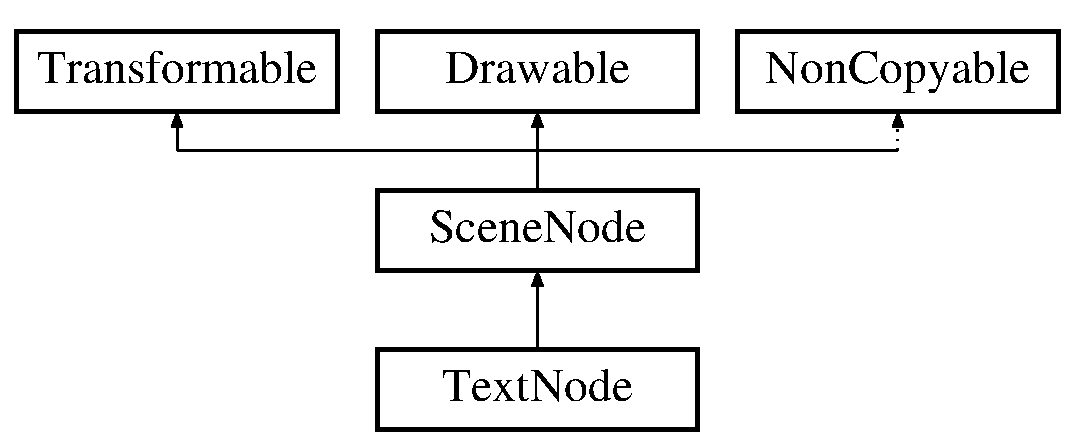
\includegraphics[height=3.000000cm]{classTextNode}
\end{center}
\end{figure}
\subsection*{Métodos públicos}
\begin{DoxyCompactItemize}
\item 
\hyperlink{classTextNode_abded9f6d861862e03a5221ea82b0e86c}{Text\+Node} (const \hyperlink{classResourceHolder}{Resource\+Holder}$<$ I\+D\+Fonts, sf\+::\+Font $>$ \&fonts, const std\+::string \&text)
\item 
void \hyperlink{classTextNode_a51c396c803287f43ee640c6b6421a212}{set\+String} (const std\+::string \&text)
\end{DoxyCompactItemize}
\subsection*{Otros miembros heredados}


\subsection{Descripción detallada}
Nodo para el dibujado de texto 

\subsection{Documentación del constructor y destructor}
\hypertarget{classTextNode_abded9f6d861862e03a5221ea82b0e86c}{}\index{Text\+Node@{Text\+Node}!Text\+Node@{Text\+Node}}
\index{Text\+Node@{Text\+Node}!Text\+Node@{Text\+Node}}
\subsubsection[{Text\+Node}]{\setlength{\rightskip}{0pt plus 5cm}Text\+Node\+::\+Text\+Node (
\begin{DoxyParamCaption}
\item[{const {\bf Resource\+Holder}$<$ I\+D\+Fonts, sf\+::\+Font $>$ \&}]{fonts, }
\item[{const std\+::string \&}]{text}
\end{DoxyParamCaption}
)}\label{classTextNode_abded9f6d861862e03a5221ea82b0e86c}
Constructor 
\begin{DoxyParams}{Parámetros}
{\em fonts} & fuentes a usar \\
\hline
{\em text} & texto a dibujar \\
\hline
\end{DoxyParams}


\subsection{Documentación de las funciones miembro}
\hypertarget{classTextNode_a51c396c803287f43ee640c6b6421a212}{}\index{Text\+Node@{Text\+Node}!set\+String@{set\+String}}
\index{set\+String@{set\+String}!Text\+Node@{Text\+Node}}
\subsubsection[{set\+String}]{\setlength{\rightskip}{0pt plus 5cm}void Text\+Node\+::set\+String (
\begin{DoxyParamCaption}
\item[{const std\+::string \&}]{text}
\end{DoxyParamCaption}
)}\label{classTextNode_a51c396c803287f43ee640c6b6421a212}
Texto a mostrar 
\begin{DoxyParams}{Parámetros}
{\em text} & texto a setear y mostrar \\
\hline
\end{DoxyParams}


La documentación para esta clase fue generada a partir de los siguientes ficheros\+:\begin{DoxyCompactItemize}
\item 
Text\+Node.\+h\item 
Text\+Node.\+cpp\end{DoxyCompactItemize}

\hypertarget{classTileMapNode}{}\section{Referencia de la Clase Tile\+Map\+Node}
\label{classTileMapNode}\index{Tile\+Map\+Node@{Tile\+Map\+Node}}


{\ttfamily \#include $<$Tile\+Map\+Node.\+h$>$}

Diagrama de herencias de Tile\+Map\+Node\begin{figure}[H]
\begin{center}
\leavevmode
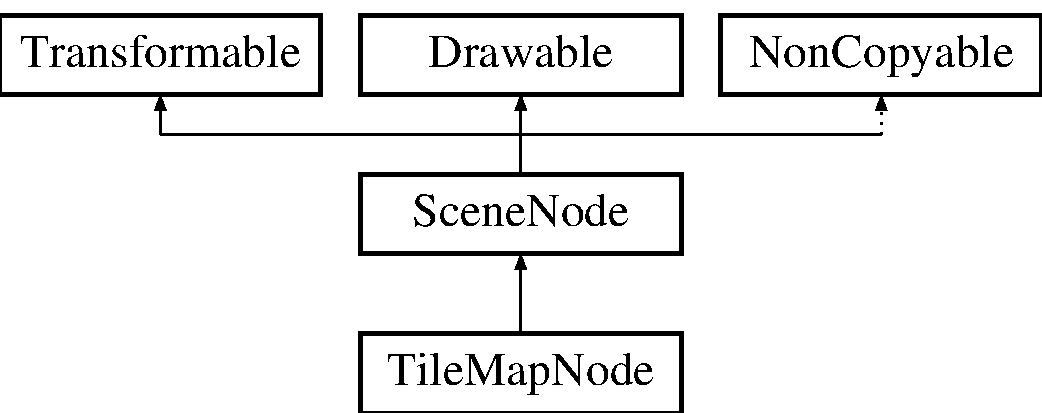
\includegraphics[height=3.000000cm]{classTileMapNode}
\end{center}
\end{figure}
\subsection*{Métodos públicos}
\begin{DoxyCompactItemize}
\item 
\hyperlink{classTileMapNode_a16e53592cfd243c14df0846539368d53}{Tile\+Map\+Node} (const \hyperlink{classResourceHolder}{Resource\+Holder}$<$ std\+::string, sf\+::\+Texture $>$ \&images, \hyperlink{structStructMap}{Struct\+Map} $\ast$map\+Info, int width, int heiht, int number\+Rows\+Visible, int number\+Columns\+Visible)
\item 
void \hyperlink{classTileMapNode_a8a2a414779f90de876e913ad172978df}{prepare\+Map} (const int $\ast$tiles\+Map)
\item 
sf\+::\+Vector2f \hyperlink{classTileMapNode_a846a4095195dc673033107c71b48e9df}{get\+Adjust\+Ratio} ()
\item 
sf\+::\+Vector2f \hyperlink{classTileMapNode_ad30b875e6c8c59efb170a67d002aaac4}{get\+Size\+Map} ()
\item 
sf\+::\+Vector2f \hyperlink{classTileMapNode_adb1c6c943363a024f3eb5b79b5e86525}{get\+Quad\+Size} ()
\item 
virtual void \hyperlink{classTileMapNode_acddf8fbc538f4952eb5ef84a211490b6}{draw\+Current} (sf\+::\+Render\+Target \&target, sf\+::\+Render\+States states) const 
\end{DoxyCompactItemize}
\subsection*{Otros miembros heredados}


\subsection{Descripción detallada}
Nodo para el dibujado del mapa 

\subsection{Documentación del constructor y destructor}
\hypertarget{classTileMapNode_a16e53592cfd243c14df0846539368d53}{}\index{Tile\+Map\+Node@{Tile\+Map\+Node}!Tile\+Map\+Node@{Tile\+Map\+Node}}
\index{Tile\+Map\+Node@{Tile\+Map\+Node}!Tile\+Map\+Node@{Tile\+Map\+Node}}
\subsubsection[{Tile\+Map\+Node}]{\setlength{\rightskip}{0pt plus 5cm}Tile\+Map\+Node\+::\+Tile\+Map\+Node (
\begin{DoxyParamCaption}
\item[{const {\bf Resource\+Holder}$<$ std\+::string, sf\+::\+Texture $>$ \&}]{images, }
\item[{{\bf Struct\+Map} $\ast$}]{map\+Info, }
\item[{int}]{width, }
\item[{int}]{heiht, }
\item[{int}]{number\+Rows\+Visible, }
\item[{int}]{number\+Columns\+Visible}
\end{DoxyParamCaption}
)}\label{classTileMapNode_a16e53592cfd243c14df0846539368d53}
Constructor 
\begin{DoxyParams}{Parámetros}
{\em images} & \\
\hline
{\em map\+Info} & \\
\hline
{\em width} & \\
\hline
{\em heiht} & \\
\hline
{\em number\+Rows\+Visible} & \\
\hline
{\em number\+Columns\+Visible} & \\
\hline
\end{DoxyParams}


\subsection{Documentación de las funciones miembro}
\hypertarget{classTileMapNode_acddf8fbc538f4952eb5ef84a211490b6}{}\index{Tile\+Map\+Node@{Tile\+Map\+Node}!draw\+Current@{draw\+Current}}
\index{draw\+Current@{draw\+Current}!Tile\+Map\+Node@{Tile\+Map\+Node}}
\subsubsection[{draw\+Current}]{\setlength{\rightskip}{0pt plus 5cm}void Tile\+Map\+Node\+::draw\+Current (
\begin{DoxyParamCaption}
\item[{sf\+::\+Render\+Target \&}]{target, }
\item[{sf\+::\+Render\+States}]{states}
\end{DoxyParamCaption}
) const\hspace{0.3cm}{\ttfamily [virtual]}}\label{classTileMapNode_acddf8fbc538f4952eb5ef84a211490b6}
Draw the actual state of the node 
\begin{DoxyParams}{Parámetros}
{\em target} & \\
\hline
{\em states} & \\
\hline
\end{DoxyParams}


Reimplementado de \hyperlink{classSceneNode}{Scene\+Node}.

\hypertarget{classTileMapNode_a846a4095195dc673033107c71b48e9df}{}\index{Tile\+Map\+Node@{Tile\+Map\+Node}!get\+Adjust\+Ratio@{get\+Adjust\+Ratio}}
\index{get\+Adjust\+Ratio@{get\+Adjust\+Ratio}!Tile\+Map\+Node@{Tile\+Map\+Node}}
\subsubsection[{get\+Adjust\+Ratio}]{\setlength{\rightskip}{0pt plus 5cm}sf\+::\+Vector2f Tile\+Map\+Node\+::get\+Adjust\+Ratio (
\begin{DoxyParamCaption}
{}
\end{DoxyParamCaption}
)\hspace{0.3cm}{\ttfamily [inline]}}\label{classTileMapNode_a846a4095195dc673033107c71b48e9df}
Devuelve el ratio de redimensionado \begin{DoxyReturn}{Devuelve}

\end{DoxyReturn}
\hypertarget{classTileMapNode_adb1c6c943363a024f3eb5b79b5e86525}{}\index{Tile\+Map\+Node@{Tile\+Map\+Node}!get\+Quad\+Size@{get\+Quad\+Size}}
\index{get\+Quad\+Size@{get\+Quad\+Size}!Tile\+Map\+Node@{Tile\+Map\+Node}}
\subsubsection[{get\+Quad\+Size}]{\setlength{\rightskip}{0pt plus 5cm}sf\+::\+Vector2f Tile\+Map\+Node\+::get\+Quad\+Size (
\begin{DoxyParamCaption}
{}
\end{DoxyParamCaption}
)\hspace{0.3cm}{\ttfamily [inline]}}\label{classTileMapNode_adb1c6c943363a024f3eb5b79b5e86525}
Devuelve el tamaño del tile en pantalla \begin{DoxyReturn}{Devuelve}

\end{DoxyReturn}
\hypertarget{classTileMapNode_ad30b875e6c8c59efb170a67d002aaac4}{}\index{Tile\+Map\+Node@{Tile\+Map\+Node}!get\+Size\+Map@{get\+Size\+Map}}
\index{get\+Size\+Map@{get\+Size\+Map}!Tile\+Map\+Node@{Tile\+Map\+Node}}
\subsubsection[{get\+Size\+Map}]{\setlength{\rightskip}{0pt plus 5cm}sf\+::\+Vector2f Tile\+Map\+Node\+::get\+Size\+Map (
\begin{DoxyParamCaption}
{}
\end{DoxyParamCaption}
)}\label{classTileMapNode_ad30b875e6c8c59efb170a67d002aaac4}
Devuelve el tamaño del mapa que se visualiza, dado por el número de columnas y filas con el tamaño del tile en ventana \begin{DoxyReturn}{Devuelve}

\end{DoxyReturn}
\hypertarget{classTileMapNode_a8a2a414779f90de876e913ad172978df}{}\index{Tile\+Map\+Node@{Tile\+Map\+Node}!prepare\+Map@{prepare\+Map}}
\index{prepare\+Map@{prepare\+Map}!Tile\+Map\+Node@{Tile\+Map\+Node}}
\subsubsection[{prepare\+Map}]{\setlength{\rightskip}{0pt plus 5cm}void Tile\+Map\+Node\+::prepare\+Map (
\begin{DoxyParamCaption}
\item[{const int $\ast$}]{tiles\+Map}
\end{DoxyParamCaption}
)}\label{classTileMapNode_a8a2a414779f90de876e913ad172978df}
Prepare the map after initialize the node with details like numbers of rows/columns, size of windows... 
\begin{DoxyParams}{Parámetros}
{\em tiles\+Map} & \\
\hline
\end{DoxyParams}


La documentación para esta clase fue generada a partir de los siguientes ficheros\+:\begin{DoxyCompactItemize}
\item 
Tile\+Map\+Node.\+h\item 
Tile\+Map\+Node.\+cpp\end{DoxyCompactItemize}

\hypertarget{classTileNode}{}\section{Referencia de la Clase Tile\+Node}
\label{classTileNode}\index{Tile\+Node@{Tile\+Node}}


{\ttfamily \#include $<$Tile\+Node.\+h$>$}

Diagrama de herencias de Tile\+Node\begin{figure}[H]
\begin{center}
\leavevmode
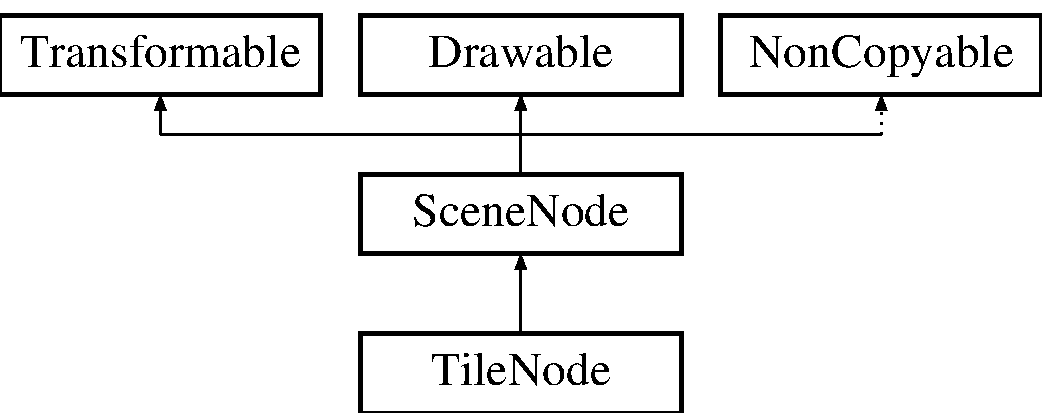
\includegraphics[height=3.000000cm]{classTileNode}
\end{center}
\end{figure}
\subsection*{Métodos públicos}
\begin{DoxyCompactItemize}
\item 
\hyperlink{classTileNode_aaa13aaf03e5e221fbec713ce849edd7d}{Tile\+Node} (const \hyperlink{classResourceHolder}{Resource\+Holder}$<$ std\+::string, sf\+::\+Texture $>$ \&images, \hyperlink{structStructMap}{Struct\+Map} $\ast$map\+Info, int width, int heiht, int number\+Rows\+Visible, int number\+Columns\+Visible)
\item 
virtual \hyperlink{classTileNode_a00c7f860dccefb4f09a43b66df52c1c8}{$\sim$\+Tile\+Node} ()
\item 
void \hyperlink{classTileNode_aab3c5946b20750e03cc754433e5996b1}{prepare\+Map} (const std\+::vector$<$ sf\+::\+Vector3i $>$ \&tiles\+Map)
\item 
sf\+::\+Vector2f \hyperlink{classTileNode_a18855e4bee1ac13ee766e8c4c676f8b0}{get\+Size\+Map} ()
\item 
sf\+::\+Vector2f \hyperlink{classTileNode_a3be8b7dad0a971c15269bbcb1fbed7de}{get\+Quad\+Size} ()
\item 
virtual void \hyperlink{classTileNode_a1e1c9f93605e91a87750f75f6a158f24}{draw\+Current} (sf\+::\+Render\+Target \&target, sf\+::\+Render\+States states) const 
\end{DoxyCompactItemize}
\subsection*{Otros miembros heredados}


\subsection{Descripción detallada}
Clase que representa un Tile o varios del mapa 

\subsection{Documentación del constructor y destructor}
\hypertarget{classTileNode_aaa13aaf03e5e221fbec713ce849edd7d}{}\index{Tile\+Node@{Tile\+Node}!Tile\+Node@{Tile\+Node}}
\index{Tile\+Node@{Tile\+Node}!Tile\+Node@{Tile\+Node}}
\subsubsection[{Tile\+Node}]{\setlength{\rightskip}{0pt plus 5cm}Tile\+Node\+::\+Tile\+Node (
\begin{DoxyParamCaption}
\item[{const {\bf Resource\+Holder}$<$ std\+::string, sf\+::\+Texture $>$ \&}]{images, }
\item[{{\bf Struct\+Map} $\ast$}]{map\+Info, }
\item[{int}]{width, }
\item[{int}]{heiht, }
\item[{int}]{number\+Rows\+Visible, }
\item[{int}]{number\+Columns\+Visible}
\end{DoxyParamCaption}
)}\label{classTileNode_aaa13aaf03e5e221fbec713ce849edd7d}

\begin{DoxyParams}{Parámetros}
{\em images} & texturas de la aplicación \\
\hline
{\em map\+Info} & estructura con la información del mapa \\
\hline
{\em width} & ancho del mapa \\
\hline
{\em heiht} & alto del mapa \\
\hline
{\em number\+Rows\+Visible} & número de filas visibles en pantalla \\
\hline
{\em number\+Columns\+Visible} & número de columnas visibles en pantalla \\
\hline
\end{DoxyParams}
\hypertarget{classTileNode_a00c7f860dccefb4f09a43b66df52c1c8}{}\index{Tile\+Node@{Tile\+Node}!````~Tile\+Node@{$\sim$\+Tile\+Node}}
\index{````~Tile\+Node@{$\sim$\+Tile\+Node}!Tile\+Node@{Tile\+Node}}
\subsubsection[{$\sim$\+Tile\+Node}]{\setlength{\rightskip}{0pt plus 5cm}Tile\+Node\+::$\sim$\+Tile\+Node (
\begin{DoxyParamCaption}
{}
\end{DoxyParamCaption}
)\hspace{0.3cm}{\ttfamily [virtual]}}\label{classTileNode_a00c7f860dccefb4f09a43b66df52c1c8}
Destructor 

\subsection{Documentación de las funciones miembro}
\hypertarget{classTileNode_a1e1c9f93605e91a87750f75f6a158f24}{}\index{Tile\+Node@{Tile\+Node}!draw\+Current@{draw\+Current}}
\index{draw\+Current@{draw\+Current}!Tile\+Node@{Tile\+Node}}
\subsubsection[{draw\+Current}]{\setlength{\rightskip}{0pt plus 5cm}void Tile\+Node\+::draw\+Current (
\begin{DoxyParamCaption}
\item[{sf\+::\+Render\+Target \&}]{target, }
\item[{sf\+::\+Render\+States}]{states}
\end{DoxyParamCaption}
) const\hspace{0.3cm}{\ttfamily [virtual]}}\label{classTileNode_a1e1c9f93605e91a87750f75f6a158f24}
Draw the actual state of the node 
\begin{DoxyParams}{Parámetros}
{\em target} & \\
\hline
{\em states} & \\
\hline
\end{DoxyParams}


Reimplementado de \hyperlink{classSceneNode}{Scene\+Node}.

\hypertarget{classTileNode_a3be8b7dad0a971c15269bbcb1fbed7de}{}\index{Tile\+Node@{Tile\+Node}!get\+Quad\+Size@{get\+Quad\+Size}}
\index{get\+Quad\+Size@{get\+Quad\+Size}!Tile\+Node@{Tile\+Node}}
\subsubsection[{get\+Quad\+Size}]{\setlength{\rightskip}{0pt plus 5cm}sf\+::\+Vector2f Tile\+Node\+::get\+Quad\+Size (
\begin{DoxyParamCaption}
{}
\end{DoxyParamCaption}
)\hspace{0.3cm}{\ttfamily [inline]}}\label{classTileNode_a3be8b7dad0a971c15269bbcb1fbed7de}
Devuelve el tamaño del tile visualizado en pantalla \begin{DoxyReturn}{Devuelve}
vector de dos números representando el tamaño 
\end{DoxyReturn}
\hypertarget{classTileNode_a18855e4bee1ac13ee766e8c4c676f8b0}{}\index{Tile\+Node@{Tile\+Node}!get\+Size\+Map@{get\+Size\+Map}}
\index{get\+Size\+Map@{get\+Size\+Map}!Tile\+Node@{Tile\+Node}}
\subsubsection[{get\+Size\+Map}]{\setlength{\rightskip}{0pt plus 5cm}sf\+::\+Vector2f Tile\+Node\+::get\+Size\+Map (
\begin{DoxyParamCaption}
{}
\end{DoxyParamCaption}
)}\label{classTileNode_a18855e4bee1ac13ee766e8c4c676f8b0}
Devuelve el tamaño del mapa \begin{DoxyReturn}{Devuelve}
vector de dos números representando el tamaño del mapa 
\end{DoxyReturn}
\hypertarget{classTileNode_aab3c5946b20750e03cc754433e5996b1}{}\index{Tile\+Node@{Tile\+Node}!prepare\+Map@{prepare\+Map}}
\index{prepare\+Map@{prepare\+Map}!Tile\+Node@{Tile\+Node}}
\subsubsection[{prepare\+Map}]{\setlength{\rightskip}{0pt plus 5cm}void Tile\+Node\+::prepare\+Map (
\begin{DoxyParamCaption}
\item[{const std\+::vector$<$ sf\+::\+Vector3i $>$ \&}]{tiles\+Map}
\end{DoxyParamCaption}
)}\label{classTileNode_aab3c5946b20750e03cc754433e5996b1}
Prepare the map after initialize the node with details like numbers of rows/columns, size of windows... 
\begin{DoxyParams}{Parámetros}
{\em tiles\+Map} & vector con los tiles. Cada tile está representado en un vector de tres enteros indicando posición x,y y el tercer entero representa el tile a dibujar \\
\hline
\end{DoxyParams}


La documentación para esta clase fue generada a partir de los siguientes ficheros\+:\begin{DoxyCompactItemize}
\item 
Tile\+Node.\+h\item 
Tile\+Node.\+cpp\end{DoxyCompactItemize}

\hypertarget{classTitleState}{}\section{Referencia de la Clase Title\+State}
\label{classTitleState}\index{Title\+State@{Title\+State}}


{\ttfamily \#include $<$Title\+State.\+h$>$}

Diagrama de herencias de Title\+State\begin{figure}[H]
\begin{center}
\leavevmode
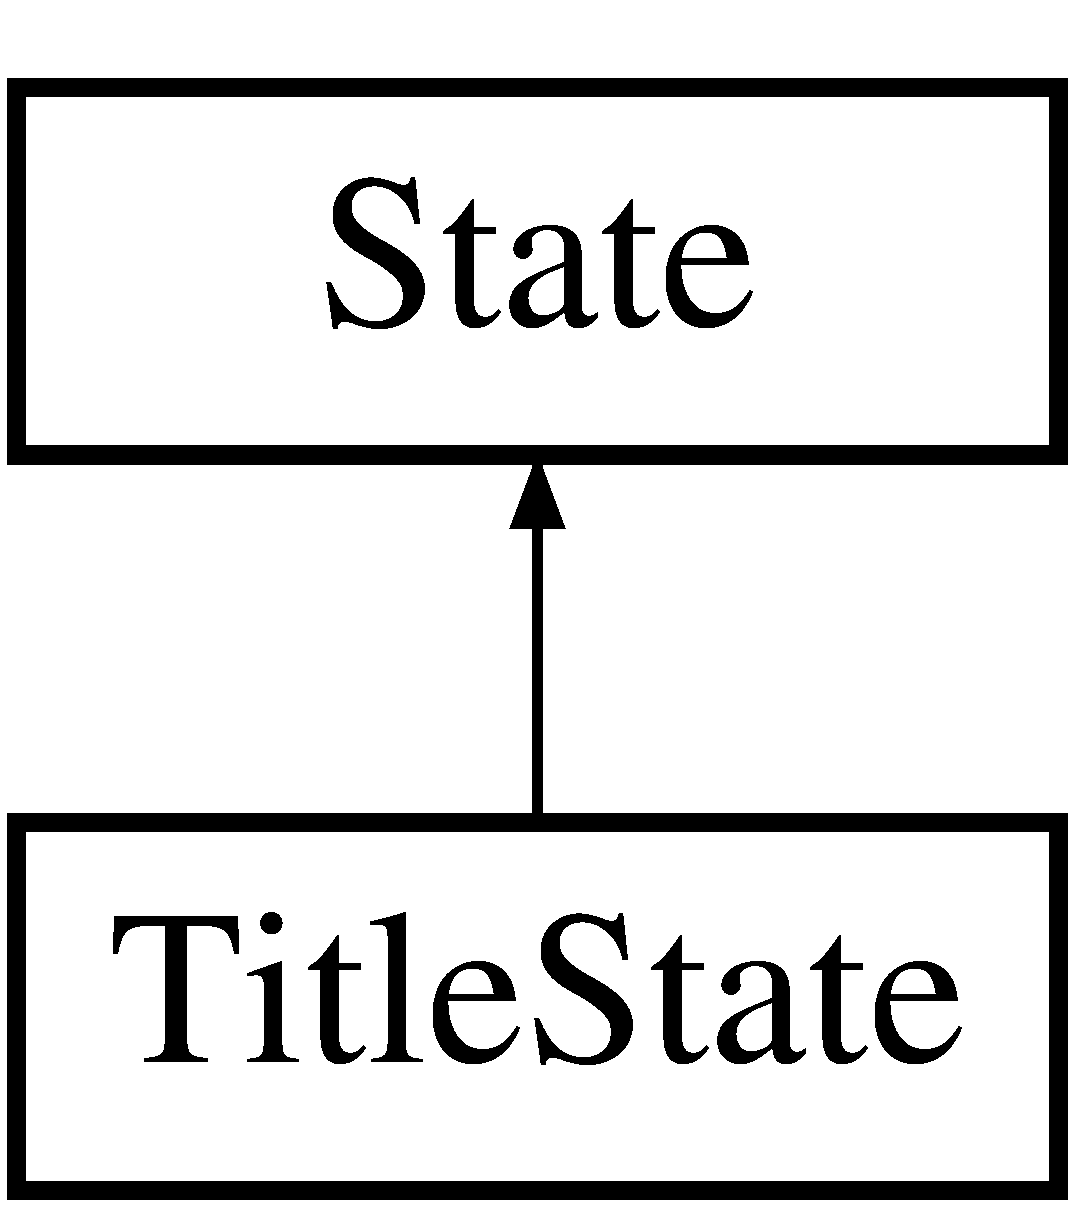
\includegraphics[height=2.000000cm]{classTitleState}
\end{center}
\end{figure}
\subsection*{Métodos públicos}
\begin{DoxyCompactItemize}
\item 
\hyperlink{classTitleState_af8f9f14886d8dbfd7c6167dcc4d3aeaf}{Title\+State} (\hyperlink{classStateStack}{State\+Stack} \&\hyperlink{classState_a86c8d3a5a1ee89896828be85a785fb04}{stack}, \hyperlink{classContext}{Context} $\ast$\hyperlink{classState_adc93e8ad3199b5891618ca88eed0436a}{context})
\item 
virtual void \hyperlink{classTitleState_ae12beafe5aad6929a56089942de1220e}{draw} ()
\item 
virtual bool \hyperlink{classTitleState_aa282ac0c6e22267cb6a7054973d75fdf}{update} (sf\+::\+Time dt)
\item 
virtual bool \hyperlink{classTitleState_a91c6ab4d741fe7445d88ed603001971a}{handle\+Event} (const sf\+::\+Event \&event)
\item 
virtual void \hyperlink{classTitleState_ab27a65d03920cbbb9cff7f14cd23372c}{pulled\+Action} ()
\item 
virtual void \hyperlink{classTitleState_a6c10b4a33cf09388f0bcca1af0872f68}{pushed\+Action} ()
\end{DoxyCompactItemize}
\subsection*{Otros miembros heredados}


\subsection{Descripción detallada}
Estado del título inicial del juego 

\subsection{Documentación del constructor y destructor}
\hypertarget{classTitleState_af8f9f14886d8dbfd7c6167dcc4d3aeaf}{}\index{Title\+State@{Title\+State}!Title\+State@{Title\+State}}
\index{Title\+State@{Title\+State}!Title\+State@{Title\+State}}
\subsubsection[{Title\+State}]{\setlength{\rightskip}{0pt plus 5cm}Title\+State\+::\+Title\+State (
\begin{DoxyParamCaption}
\item[{{\bf State\+Stack} \&}]{stack, }
\item[{{\bf Context} $\ast$}]{context}
\end{DoxyParamCaption}
)}\label{classTitleState_af8f9f14886d8dbfd7c6167dcc4d3aeaf}
Constructor 
\begin{DoxyParams}{Parámetros}
{\em stack} & pila de estados \\
\hline
{\em context} & contexto \\
\hline
\end{DoxyParams}


\subsection{Documentación de las funciones miembro}
\hypertarget{classTitleState_ae12beafe5aad6929a56089942de1220e}{}\index{Title\+State@{Title\+State}!draw@{draw}}
\index{draw@{draw}!Title\+State@{Title\+State}}
\subsubsection[{draw}]{\setlength{\rightskip}{0pt plus 5cm}void Title\+State\+::draw (
\begin{DoxyParamCaption}
{}
\end{DoxyParamCaption}
)\hspace{0.3cm}{\ttfamily [virtual]}}\label{classTitleState_ae12beafe5aad6929a56089942de1220e}
Dibuja el estado 

Implementa \hyperlink{classState_ae261605bc40b7e3959ce5df5457e4942}{State}.

\hypertarget{classTitleState_a91c6ab4d741fe7445d88ed603001971a}{}\index{Title\+State@{Title\+State}!handle\+Event@{handle\+Event}}
\index{handle\+Event@{handle\+Event}!Title\+State@{Title\+State}}
\subsubsection[{handle\+Event}]{\setlength{\rightskip}{0pt plus 5cm}bool Title\+State\+::handle\+Event (
\begin{DoxyParamCaption}
\item[{const sf\+::\+Event \&}]{event}
\end{DoxyParamCaption}
)\hspace{0.3cm}{\ttfamily [virtual]}}\label{classTitleState_a91c6ab4d741fe7445d88ed603001971a}
Procesa la entrada del usuario 
\begin{DoxyParams}{Parámetros}
{\em event} & evento \\
\hline
\end{DoxyParams}
\begin{DoxyReturn}{Devuelve}
true si lo ha procesado, false si no (o lo ha procesado pero que continúe) 
\end{DoxyReturn}


Implementa \hyperlink{classState_a19965f83460b248c42952aac8d001206}{State}.

\hypertarget{classTitleState_ab27a65d03920cbbb9cff7f14cd23372c}{}\index{Title\+State@{Title\+State}!pulled\+Action@{pulled\+Action}}
\index{pulled\+Action@{pulled\+Action}!Title\+State@{Title\+State}}
\subsubsection[{pulled\+Action}]{\setlength{\rightskip}{0pt plus 5cm}void Title\+State\+::pulled\+Action (
\begin{DoxyParamCaption}
{}
\end{DoxyParamCaption}
)\hspace{0.3cm}{\ttfamily [virtual]}}\label{classTitleState_ab27a65d03920cbbb9cff7f14cd23372c}
Método ejecutado cuando es sacado de la pila 

Reimplementado de \hyperlink{classState_a92620c4648de675037b20ec59edb52a3}{State}.

\hypertarget{classTitleState_a6c10b4a33cf09388f0bcca1af0872f68}{}\index{Title\+State@{Title\+State}!pushed\+Action@{pushed\+Action}}
\index{pushed\+Action@{pushed\+Action}!Title\+State@{Title\+State}}
\subsubsection[{pushed\+Action}]{\setlength{\rightskip}{0pt plus 5cm}void Title\+State\+::pushed\+Action (
\begin{DoxyParamCaption}
{}
\end{DoxyParamCaption}
)\hspace{0.3cm}{\ttfamily [virtual]}}\label{classTitleState_a6c10b4a33cf09388f0bcca1af0872f68}
Método ejecutado cuando es puesto en pila 

Reimplementado de \hyperlink{classState_a3cc6a1378f32f9ed6a2d1d8140296808}{State}.

\hypertarget{classTitleState_aa282ac0c6e22267cb6a7054973d75fdf}{}\index{Title\+State@{Title\+State}!update@{update}}
\index{update@{update}!Title\+State@{Title\+State}}
\subsubsection[{update}]{\setlength{\rightskip}{0pt plus 5cm}bool Title\+State\+::update (
\begin{DoxyParamCaption}
\item[{sf\+::\+Time}]{delta}
\end{DoxyParamCaption}
)\hspace{0.3cm}{\ttfamily [virtual]}}\label{classTitleState_aa282ac0c6e22267cb6a7054973d75fdf}
Actualiza el estado 
\begin{DoxyParams}{Parámetros}
{\em delta} & tiempo entre frame y frame \\
\hline
\end{DoxyParams}
\begin{DoxyReturn}{Devuelve}
true si se ha actualizado 
\end{DoxyReturn}


Implementa \hyperlink{classState_aa6366828eb50639e86b94008cfad9c5d}{State}.



La documentación para esta clase fue generada a partir de los siguientes ficheros\+:\begin{DoxyCompactItemize}
\item 
Title\+State.\+h\item 
Title\+State.\+cpp\end{DoxyCompactItemize}

\hypertarget{classTProperty}{}\section{Referencia de la plantilla de la Clase T\+Property$<$ T\+Y\+P\+E $>$}
\label{classTProperty}\index{T\+Property$<$ T\+Y\+P\+E $>$@{T\+Property$<$ T\+Y\+P\+E $>$}}
Diagrama de herencias de T\+Property$<$ T\+Y\+P\+E $>$\begin{figure}[H]
\begin{center}
\leavevmode
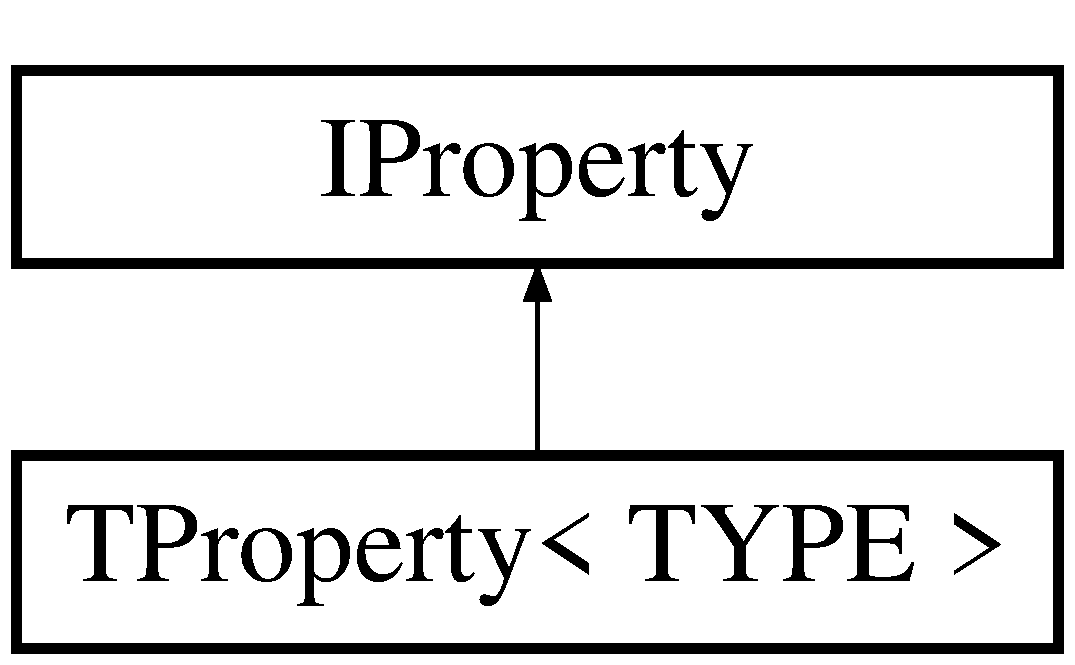
\includegraphics[height=2.000000cm]{classTProperty}
\end{center}
\end{figure}
\subsection*{Métodos públicos}
\begin{DoxyCompactItemize}
\item 
\hyperlink{classTProperty_a58ede57ac36a9c98bb06ca773f9b62ee}{T\+Property} (const std\+::string the\+Property\+I\+D)
\item 
T\+Y\+P\+E \hyperlink{classTProperty_adceda6e9d1c01f091cec619a48b1822f}{Get\+Value} ()
\item 
void \hyperlink{classTProperty_ad7949c54d792c67cd73b299964699541}{Set\+Value} (T\+Y\+P\+E the\+Value)
\item 
void \hyperlink{classTProperty_ab463fc86cb27252b763b38be21e82c3f}{Update} ()
\item 
\hyperlink{classIProperty}{I\+Property} $\ast$ \hyperlink{classTProperty_a40e392d305cc3886255946359977edcb}{Make\+Clone} ()
\end{DoxyCompactItemize}
\subsection*{Otros miembros heredados}


\subsection{Documentación del constructor y destructor}
\hypertarget{classTProperty_a58ede57ac36a9c98bb06ca773f9b62ee}{}\index{T\+Property@{T\+Property}!T\+Property@{T\+Property}}
\index{T\+Property@{T\+Property}!T\+Property@{T\+Property}}
\subsubsection[{T\+Property}]{\setlength{\rightskip}{0pt plus 5cm}template$<$class T\+Y\+P\+E = unsigned int$>$ {\bf T\+Property}$<$ T\+Y\+P\+E $>$\+::{\bf T\+Property} (
\begin{DoxyParamCaption}
\item[{const std\+::string}]{the\+Property\+I\+D}
\end{DoxyParamCaption}
)\hspace{0.3cm}{\ttfamily [inline]}}\label{classTProperty_a58ede57ac36a9c98bb06ca773f9b62ee}
\hyperlink{classTProperty}{T\+Property} default constructor 
\begin{DoxyParams}[1]{Parámetros}
\mbox{\tt in}  & {\em the\+Property\+I\+D} & to use for this property \\
\hline
\end{DoxyParams}


\subsection{Documentación de las funciones miembro}
\hypertarget{classTProperty_adceda6e9d1c01f091cec619a48b1822f}{}\index{T\+Property@{T\+Property}!Get\+Value@{Get\+Value}}
\index{Get\+Value@{Get\+Value}!T\+Property@{T\+Property}}
\subsubsection[{Get\+Value}]{\setlength{\rightskip}{0pt plus 5cm}template$<$class T\+Y\+P\+E = unsigned int$>$ T\+Y\+P\+E {\bf T\+Property}$<$ T\+Y\+P\+E $>$\+::Get\+Value (
\begin{DoxyParamCaption}
{}
\end{DoxyParamCaption}
)\hspace{0.3cm}{\ttfamily [inline]}}\label{classTProperty_adceda6e9d1c01f091cec619a48b1822f}
Get\+Value will return the property value \begin{DoxyReturn}{Devuelve}
the property value 
\end{DoxyReturn}
\hypertarget{classTProperty_a40e392d305cc3886255946359977edcb}{}\index{T\+Property@{T\+Property}!Make\+Clone@{Make\+Clone}}
\index{Make\+Clone@{Make\+Clone}!T\+Property@{T\+Property}}
\subsubsection[{Make\+Clone}]{\setlength{\rightskip}{0pt plus 5cm}template$<$class T\+Y\+P\+E = unsigned int$>$ {\bf I\+Property}$\ast$ {\bf T\+Property}$<$ T\+Y\+P\+E $>$\+::Make\+Clone (
\begin{DoxyParamCaption}
{}
\end{DoxyParamCaption}
)\hspace{0.3cm}{\ttfamily [inline]}, {\ttfamily [virtual]}}\label{classTProperty_a40e392d305cc3886255946359977edcb}
Make\+Clone is responsible for creating a clone of this \hyperlink{classIProperty}{I\+Property} derived class and returning it as part of the Prototype and Instance system. The value of the Property will also be copied into the clone. \begin{DoxyReturn}{Devuelve}
pointer to the \hyperlink{classIProperty}{I\+Property} derived class clone that was created 
\end{DoxyReturn}


Implementa \hyperlink{classIProperty_a5ae2b99d460cc149f4afa04e9d97d584}{I\+Property}.

\hypertarget{classTProperty_ad7949c54d792c67cd73b299964699541}{}\index{T\+Property@{T\+Property}!Set\+Value@{Set\+Value}}
\index{Set\+Value@{Set\+Value}!T\+Property@{T\+Property}}
\subsubsection[{Set\+Value}]{\setlength{\rightskip}{0pt plus 5cm}template$<$class T\+Y\+P\+E = unsigned int$>$ void {\bf T\+Property}$<$ T\+Y\+P\+E $>$\+::Set\+Value (
\begin{DoxyParamCaption}
\item[{T\+Y\+P\+E}]{the\+Value}
\end{DoxyParamCaption}
)\hspace{0.3cm}{\ttfamily [inline]}}\label{classTProperty_ad7949c54d792c67cd73b299964699541}
Set\+Value will set the property value to the value provided. \hypertarget{classTProperty_ab463fc86cb27252b763b38be21e82c3f}{}\index{T\+Property@{T\+Property}!Update@{Update}}
\index{Update@{Update}!T\+Property@{T\+Property}}
\subsubsection[{Update}]{\setlength{\rightskip}{0pt plus 5cm}template$<$class T\+Y\+P\+E = unsigned int$>$ void {\bf T\+Property}$<$ T\+Y\+P\+E $>$\+::Update (
\begin{DoxyParamCaption}
{}
\end{DoxyParamCaption}
)\hspace{0.3cm}{\ttfamily [inline]}, {\ttfamily [virtual]}}\label{classTProperty_ab463fc86cb27252b763b38be21e82c3f}
Update will be called giving each property a chance to change itself during the Update phase of the Game\+Loop (see I\+Entity\+::\+Update\+Fixed) 

Implementa \hyperlink{classIProperty_af257f5c126fedd5ad89726cdeeccbc0a}{I\+Property}.



La documentación para esta clase fue generada a partir del siguiente fichero\+:\begin{DoxyCompactItemize}
\item 
T\+Property.\+h\end{DoxyCompactItemize}

\hypertarget{structTransition}{}\section{Referencia de la Estructura Transition}
\label{structTransition}\index{Transition@{Transition}}


{\ttfamily \#include $<$State\+Machine.\+h$>$}

\subsection*{Métodos públicos}
\begin{DoxyCompactItemize}
\item 
\hypertarget{structTransition_a8ff1179926e5771d232d81961ac69017}{}{\bfseries Transition} (int \hyperlink{structTransition_ad7509cc6401e1038e17dbeea187c15ca}{state}, int \hyperlink{structTransition_a71bfb2883c7991812e7fb3b34e258aab}{entry}, int \hyperlink{structTransition_a423a2791bbcafadc339eaa3da7c7fb04}{new\+State})\label{structTransition_a8ff1179926e5771d232d81961ac69017}

\end{DoxyCompactItemize}
\subsection*{Campos de datos}
\begin{DoxyCompactItemize}
\item 
int \hyperlink{structTransition_ad7509cc6401e1038e17dbeea187c15ca}{state}
\item 
int \hyperlink{structTransition_a71bfb2883c7991812e7fb3b34e258aab}{entry}
\item 
int \hyperlink{structTransition_a423a2791bbcafadc339eaa3da7c7fb04}{new\+State}
\end{DoxyCompactItemize}


\subsection{Descripción detallada}
Estructura de transición para la máquina de estados finitos 

\subsection{Documentación de los campos}
\hypertarget{structTransition_a71bfb2883c7991812e7fb3b34e258aab}{}\index{Transition@{Transition}!entry@{entry}}
\index{entry@{entry}!Transition@{Transition}}
\subsubsection[{entry}]{\setlength{\rightskip}{0pt plus 5cm}int Transition\+::entry}\label{structTransition_a71bfb2883c7991812e7fb3b34e258aab}
Entrada \hypertarget{structTransition_a423a2791bbcafadc339eaa3da7c7fb04}{}\index{Transition@{Transition}!new\+State@{new\+State}}
\index{new\+State@{new\+State}!Transition@{Transition}}
\subsubsection[{new\+State}]{\setlength{\rightskip}{0pt plus 5cm}int Transition\+::new\+State}\label{structTransition_a423a2791bbcafadc339eaa3da7c7fb04}
Nuevo estado \hypertarget{structTransition_ad7509cc6401e1038e17dbeea187c15ca}{}\index{Transition@{Transition}!state@{state}}
\index{state@{state}!Transition@{Transition}}
\subsubsection[{state}]{\setlength{\rightskip}{0pt plus 5cm}int Transition\+::state}\label{structTransition_ad7509cc6401e1038e17dbeea187c15ca}
Estado previo 

La documentación para esta estructura fue generada a partir del siguiente fichero\+:\begin{DoxyCompactItemize}
\item 
State\+Machine.\+h\end{DoxyCompactItemize}

\hypertarget{structTriangle}{}\section{Referencia de la Estructura Triangle}
\label{structTriangle}\index{Triangle@{Triangle}}


{\ttfamily \#include $<$Triangle.\+h$>$}

\subsection*{Métodos públicos}
\begin{DoxyCompactItemize}
\item 
\hyperlink{structTriangle_adfb983e02cc6901f9cf28c81036f8dce}{Triangle} (sf\+::\+Vector2f \&p0, sf\+::\+Vector2f \&p1, sf\+::\+Vector2f \&p2)
\item 
\hyperlink{structTriangle_aaefe4ed500c07918d30c6f0e286332c5}{Triangle} ()
\item 
bool \hyperlink{structTriangle_a6e233369dff883d425b1077c4eb1fb39}{point\+Inside} (sf\+::\+Vector2f \&point)
\item 
sf\+::\+Float\+Rect \hyperlink{structTriangle_ad65472004d16c530d7a55713f7e9cf29}{get\+Bounds} ()
\item 
bool \hyperlink{structTriangle_a8329a43d14d395c4cf7beb79014a5300}{aabb\+Collision} (sf\+::\+Float\+Rect \&one\+Rect)
\item 
bool \hyperlink{structTriangle_ab4526a1cd59654ac9018c445ccbc0080}{triangle\+V\+S\+Triangle} (\hyperlink{structTriangle}{Triangle} \&triangle)
\end{DoxyCompactItemize}
\subsection*{Campos de datos}
\begin{DoxyCompactItemize}
\item 
\hypertarget{structTriangle_a329348e606ae7d13277e4990ab636054}{}sf\+::\+Vector2f {\bfseries p0}\label{structTriangle_a329348e606ae7d13277e4990ab636054}

\item 
\hypertarget{structTriangle_adb0caecb15df48f0d5bcfe3000ed9ee3}{}sf\+::\+Vector2f {\bfseries p1}\label{structTriangle_adb0caecb15df48f0d5bcfe3000ed9ee3}

\item 
\hypertarget{structTriangle_af1832d337761d4949cabaff62e9b7711}{}sf\+::\+Vector2f {\bfseries p2}\label{structTriangle_af1832d337761d4949cabaff62e9b7711}

\end{DoxyCompactItemize}


\subsection{Descripción detallada}
Estructura de un triángulo 

\subsection{Documentación del constructor y destructor}
\hypertarget{structTriangle_adfb983e02cc6901f9cf28c81036f8dce}{}\index{Triangle@{Triangle}!Triangle@{Triangle}}
\index{Triangle@{Triangle}!Triangle@{Triangle}}
\subsubsection[{Triangle}]{\setlength{\rightskip}{0pt plus 5cm}Triangle\+::\+Triangle (
\begin{DoxyParamCaption}
\item[{sf\+::\+Vector2f \&}]{p0, }
\item[{sf\+::\+Vector2f \&}]{p1, }
\item[{sf\+::\+Vector2f \&}]{p2}
\end{DoxyParamCaption}
)\hspace{0.3cm}{\ttfamily [inline]}}\label{structTriangle_adfb983e02cc6901f9cf28c81036f8dce}
Constructor, construye un triángulo a partir de tres puntos 
\begin{DoxyParams}{Parámetros}
{\em p0} & un punto \\
\hline
{\em p1} & segundo punto \\
\hline
{\em p2} & tercer punto \\
\hline
\end{DoxyParams}
\hypertarget{structTriangle_aaefe4ed500c07918d30c6f0e286332c5}{}\index{Triangle@{Triangle}!Triangle@{Triangle}}
\index{Triangle@{Triangle}!Triangle@{Triangle}}
\subsubsection[{Triangle}]{\setlength{\rightskip}{0pt plus 5cm}Triangle\+::\+Triangle (
\begin{DoxyParamCaption}
{}
\end{DoxyParamCaption}
)\hspace{0.3cm}{\ttfamily [inline]}}\label{structTriangle_aaefe4ed500c07918d30c6f0e286332c5}
Triángulo por defecto 

\subsection{Documentación de las funciones miembro}
\hypertarget{structTriangle_a8329a43d14d395c4cf7beb79014a5300}{}\index{Triangle@{Triangle}!aabb\+Collision@{aabb\+Collision}}
\index{aabb\+Collision@{aabb\+Collision}!Triangle@{Triangle}}
\subsubsection[{aabb\+Collision}]{\setlength{\rightskip}{0pt plus 5cm}bool Triangle\+::aabb\+Collision (
\begin{DoxyParamCaption}
\item[{sf\+::\+Float\+Rect \&}]{one\+Rect}
\end{DoxyParamCaption}
)\hspace{0.3cm}{\ttfamily [inline]}}\label{structTriangle_a8329a43d14d395c4cf7beb79014a5300}
Testea la colisión entre el triángulo y el rectángulo dado 
\begin{DoxyParams}{Parámetros}
{\em one\+Rect} & rectángulo a testear \\
\hline
\end{DoxyParams}
\begin{DoxyReturn}{Devuelve}
true si colisionan 
\end{DoxyReturn}
\hypertarget{structTriangle_ad65472004d16c530d7a55713f7e9cf29}{}\index{Triangle@{Triangle}!get\+Bounds@{get\+Bounds}}
\index{get\+Bounds@{get\+Bounds}!Triangle@{Triangle}}
\subsubsection[{get\+Bounds}]{\setlength{\rightskip}{0pt plus 5cm}sf\+::\+Float\+Rect Triangle\+::get\+Bounds (
\begin{DoxyParamCaption}
{}
\end{DoxyParamCaption}
)\hspace{0.3cm}{\ttfamily [inline]}}\label{structTriangle_ad65472004d16c530d7a55713f7e9cf29}
Devuelve un rectángulo que contenga el triángulo \begin{DoxyReturn}{Devuelve}
un rectángulo 
\end{DoxyReturn}
\hypertarget{structTriangle_a6e233369dff883d425b1077c4eb1fb39}{}\index{Triangle@{Triangle}!point\+Inside@{point\+Inside}}
\index{point\+Inside@{point\+Inside}!Triangle@{Triangle}}
\subsubsection[{point\+Inside}]{\setlength{\rightskip}{0pt plus 5cm}bool Triangle\+::point\+Inside (
\begin{DoxyParamCaption}
\item[{sf\+::\+Vector2f \&}]{point}
\end{DoxyParamCaption}
)\hspace{0.3cm}{\ttfamily [inline]}}\label{structTriangle_a6e233369dff883d425b1077c4eb1fb39}
Comprueba si el punto dado está dentro del triángulo 
\begin{DoxyParams}{Parámetros}
{\em point} & punto a testear \\
\hline
\end{DoxyParams}
\begin{DoxyReturn}{Devuelve}
true si el punto está dentro del triángulo 
\end{DoxyReturn}
\hypertarget{structTriangle_ab4526a1cd59654ac9018c445ccbc0080}{}\index{Triangle@{Triangle}!triangle\+V\+S\+Triangle@{triangle\+V\+S\+Triangle}}
\index{triangle\+V\+S\+Triangle@{triangle\+V\+S\+Triangle}!Triangle@{Triangle}}
\subsubsection[{triangle\+V\+S\+Triangle}]{\setlength{\rightskip}{0pt plus 5cm}bool Triangle\+::triangle\+V\+S\+Triangle (
\begin{DoxyParamCaption}
\item[{{\bf Triangle} \&}]{triangle}
\end{DoxyParamCaption}
)\hspace{0.3cm}{\ttfamily [inline]}}\label{structTriangle_ab4526a1cd59654ac9018c445ccbc0080}
Testea la colisión entre el triángulo y otro triángulo dado 
\begin{DoxyParams}{Parámetros}
{\em triangle} & triangulo a comprobrar \\
\hline
\end{DoxyParams}
\begin{DoxyReturn}{Devuelve}
true si colisionan 
\end{DoxyReturn}


La documentación para esta estructura fue generada a partir del siguiente fichero\+:\begin{DoxyCompactItemize}
\item 
Triangle.\+h\end{DoxyCompactItemize}

\hypertarget{classIProperty_1_1Type__t}{}\section{Referencia de la Clase I\+Property\+:\+:Type\+\_\+t}
\label{classIProperty_1_1Type__t}\index{I\+Property\+::\+Type\+\_\+t@{I\+Property\+::\+Type\+\_\+t}}
\subsection*{Métodos públicos}
\begin{DoxyCompactItemize}
\item 
\hypertarget{classIProperty_1_1Type__t_a9cf5cd01fde258a89672f0ec5a0b2a71}{}{\bfseries Type\+\_\+t} (std\+::string the\+Name)\label{classIProperty_1_1Type__t_a9cf5cd01fde258a89672f0ec5a0b2a71}

\item 
\hypertarget{classIProperty_1_1Type__t_ad7ab65f192478f0487c5194e739f906c}{}std\+::string {\bfseries Name} () const \label{classIProperty_1_1Type__t_ad7ab65f192478f0487c5194e739f906c}

\end{DoxyCompactItemize}


La documentación para esta clase fue generada a partir del siguiente fichero\+:\begin{DoxyCompactItemize}
\item 
I\+Property.\+h\end{DoxyCompactItemize}

\hypertarget{classVector}{}\section{Referencia de la Clase Vector}
\label{classVector}\index{Vector@{Vector}}


{\ttfamily \#include $<$Vector.\+h$>$}

\subsection*{Métodos públicos}
\begin{DoxyCompactItemize}
\item 
\hyperlink{classVector_a6f80c73b5f18dcf3f8e36065bdc8b9e5}{Vector} ()
\item 
\hyperlink{classVector_a7b248851572c39229270f04c3dd192d8}{Vector} (float \hyperlink{classVector_aca49165049a1e21ae47afcfc078819ed}{x}, float \hyperlink{classVector_a81be9102fca6d9beea3efef522c4c09d}{y})
\item 
void \hyperlink{classVector_a0cc91580a3011a9eebda448ff4c6e71d}{zero} ()
\item 
void \hyperlink{classVector_acc4fab345402e8979203dbc9ac1a8aea}{negate} ()
\item 
void \hyperlink{classVector_a4b5f64de730e759afc88fd53e98d3c1b}{add} (const \hyperlink{classVector}{Vector} \&vector)
\item 
void \hyperlink{classVector_ac0f345b85e9fff7cfbcbf991c169098c}{subtract} (const \hyperlink{classVector}{Vector} \&vector)
\item 
void \hyperlink{classVector_a3e8105767c84093c371ea87d13884fd0}{multiply} (float scalar)
\item 
void \hyperlink{classVector_ad1cdb507ea463624b707df32f44ca1cf}{divide} (float scalar)
\item 
float \hyperlink{classVector_a6085c16ca644e4530b1e0c618fab556f}{dot} (const \hyperlink{classVector}{Vector} \&vector) const 
\item 
\hypertarget{classVector_a42cd8aa8e911feefd505634eb6efdcc6}{}\hyperlink{classVector}{Vector} {\bfseries cross} (float s)\label{classVector_a42cd8aa8e911feefd505634eb6efdcc6}

\item 
float \hyperlink{classVector_ad7d03652023753f76a5a426abf221128}{length\+Squared} () const 
\item 
float \hyperlink{classVector_a41bd7eef3dfc5832eda40ea2a59bb9f5}{length} () const 
\item 
\hyperlink{classVector}{Vector} \& \hyperlink{classVector_a7586a8c96e492a72418191a0300f3123}{normalize} ()
\item 
\hyperlink{classVector}{Vector} \hyperlink{classVector_aca2765e0e086de29cd95fb97bc384599}{unit} () const 
\item 
bool \hyperlink{classVector_a66636f72a92a9746e6f080593356cae9}{normalized} () const 
\item 
bool \hyperlink{classVector_a164aa24033c4cb6a23fa69902dcbf1f5}{operator==} (const \hyperlink{classVector}{Vector} \&other) const 
\item 
bool \hyperlink{classVector_af7382cb07df79766f0f773f8b64c8312}{operator!=} (const \hyperlink{classVector}{Vector} \&other) const 
\item 
float \& \hyperlink{classVector_a950c7b6666b92ab5b5b9af29e19067c1}{operator\mbox{[}$\,$\mbox{]}} (int i)
\item 
const float \& \hyperlink{classVector_aa5b3b63a6d6dd7f381d37789bec33848}{operator\mbox{[}$\,$\mbox{]}} (int i) const 
\end{DoxyCompactItemize}
\subsection*{Campos de datos}
\begin{DoxyCompactItemize}
\item 
\hypertarget{classVector_aca49165049a1e21ae47afcfc078819ed}{}float \hyperlink{classVector_aca49165049a1e21ae47afcfc078819ed}{x}\label{classVector_aca49165049a1e21ae47afcfc078819ed}

\begin{DoxyCompactList}\small\item\em x component of vector \end{DoxyCompactList}\item 
\hypertarget{classVector_a81be9102fca6d9beea3efef522c4c09d}{}float \hyperlink{classVector_a81be9102fca6d9beea3efef522c4c09d}{y}\label{classVector_a81be9102fca6d9beea3efef522c4c09d}

\begin{DoxyCompactList}\small\item\em y component of vector \end{DoxyCompactList}\end{DoxyCompactItemize}
\subsection*{Amigas}
\begin{DoxyCompactItemize}
\item 
\hypertarget{classVector_abf2b446e7047f3f0556b53e4ce7868d0}{}\hyperlink{classVector}{Vector} {\bfseries operator-\/} (const \hyperlink{classVector}{Vector} \&a)\label{classVector_abf2b446e7047f3f0556b53e4ce7868d0}

\item 
\hypertarget{classVector_a53d6a19cb17320a43a60e4356f80c205}{}\hyperlink{classVector}{Vector} {\bfseries operator+} (const \hyperlink{classVector}{Vector} \&a, const \hyperlink{classVector}{Vector} \&b)\label{classVector_a53d6a19cb17320a43a60e4356f80c205}

\item 
\hypertarget{classVector_a316d381a8ae7de1d299f2131a042a349}{}\hyperlink{classVector}{Vector} {\bfseries operator-\/} (const \hyperlink{classVector}{Vector} \&a, const \hyperlink{classVector}{Vector} \&b)\label{classVector_a316d381a8ae7de1d299f2131a042a349}

\item 
\hypertarget{classVector_a4fb2d244db84da243c5931a907fedb45}{}\hyperlink{classVector}{Vector} \& {\bfseries operator+=} (\hyperlink{classVector}{Vector} \&a, const \hyperlink{classVector}{Vector} \&b)\label{classVector_a4fb2d244db84da243c5931a907fedb45}

\item 
\hypertarget{classVector_ade89f1f57dfe0f62585d061044d01ae4}{}\hyperlink{classVector}{Vector} \& {\bfseries operator-\/=} (\hyperlink{classVector}{Vector} \&a, const \hyperlink{classVector}{Vector} \&b)\label{classVector_ade89f1f57dfe0f62585d061044d01ae4}

\item 
\hypertarget{classVector_a0bad8928a0e05294b614b3843cfe63a2}{}\hyperlink{classVector}{Vector} {\bfseries operator$\ast$} (const \hyperlink{classVector}{Vector} \&a, float s)\label{classVector_a0bad8928a0e05294b614b3843cfe63a2}

\item 
\hypertarget{classVector_a5d3b08c505c7eae71de50dbb3d21a5cf}{}\hyperlink{classVector}{Vector} {\bfseries operator/} (const \hyperlink{classVector}{Vector} \&a, float s)\label{classVector_a5d3b08c505c7eae71de50dbb3d21a5cf}

\item 
\hypertarget{classVector_a0643b5488c2ae01d7c78a9c2939c7601}{}\hyperlink{classVector}{Vector} \& {\bfseries operator$\ast$=} (\hyperlink{classVector}{Vector} \&a, float s)\label{classVector_a0643b5488c2ae01d7c78a9c2939c7601}

\item 
\hypertarget{classVector_a28d8f00719ae1134b082c4c40ad10167}{}\hyperlink{classVector}{Vector} \& {\bfseries operator/=} (\hyperlink{classVector}{Vector} \&a, float s)\label{classVector_a28d8f00719ae1134b082c4c40ad10167}

\item 
\hypertarget{classVector_a2e971b56ee4f7f7743269f21f43fbdba}{}\hyperlink{classVector}{Vector} {\bfseries operator$\ast$} (float s, const \hyperlink{classVector}{Vector} \&a)\label{classVector_a2e971b56ee4f7f7743269f21f43fbdba}

\item 
\hypertarget{classVector_aee36ca7f6efa7cc808e5d6ed523f965b}{}\hyperlink{classVector}{Vector} \& {\bfseries operator$\ast$=} (float s, \hyperlink{classVector}{Vector} \&a)\label{classVector_aee36ca7f6efa7cc808e5d6ed523f965b}

\end{DoxyCompactItemize}


\subsection{Descripción detallada}
Clase representando un vector de dos puntos y en el que se han sobreescrito operadores a conveniencia para su uso en colisiones. 

\subsection{Documentación del constructor y destructor}
\hypertarget{classVector_a6f80c73b5f18dcf3f8e36065bdc8b9e5}{}\index{Vector@{Vector}!Vector@{Vector}}
\index{Vector@{Vector}!Vector@{Vector}}
\subsubsection[{Vector}]{\setlength{\rightskip}{0pt plus 5cm}Vector\+::\+Vector (
\begin{DoxyParamCaption}
{}
\end{DoxyParamCaption}
)\hspace{0.3cm}{\ttfamily [inline]}}\label{classVector_a6f80c73b5f18dcf3f8e36065bdc8b9e5}
default constructor. does nothing for speed. \hypertarget{classVector_a7b248851572c39229270f04c3dd192d8}{}\index{Vector@{Vector}!Vector@{Vector}}
\index{Vector@{Vector}!Vector@{Vector}}
\subsubsection[{Vector}]{\setlength{\rightskip}{0pt plus 5cm}Vector\+::\+Vector (
\begin{DoxyParamCaption}
\item[{float}]{x, }
\item[{float}]{y}
\end{DoxyParamCaption}
)\hspace{0.3cm}{\ttfamily [inline]}}\label{classVector_a7b248851572c39229270f04c3dd192d8}
construct vector from x,y components. 
\begin{DoxyParams}{Parámetros}
{\em x} & \\
\hline
{\em y} & \\
\hline
\end{DoxyParams}


\subsection{Documentación de las funciones miembro}
\hypertarget{classVector_a4b5f64de730e759afc88fd53e98d3c1b}{}\index{Vector@{Vector}!add@{add}}
\index{add@{add}!Vector@{Vector}}
\subsubsection[{add}]{\setlength{\rightskip}{0pt plus 5cm}void Vector\+::add (
\begin{DoxyParamCaption}
\item[{const {\bf Vector} \&}]{vector}
\end{DoxyParamCaption}
)\hspace{0.3cm}{\ttfamily [inline]}}\label{classVector_a4b5f64de730e759afc88fd53e98d3c1b}
add another vector to this vector. 
\begin{DoxyParams}{Parámetros}
{\em vector} & \\
\hline
\end{DoxyParams}
\hypertarget{classVector_ad1cdb507ea463624b707df32f44ca1cf}{}\index{Vector@{Vector}!divide@{divide}}
\index{divide@{divide}!Vector@{Vector}}
\subsubsection[{divide}]{\setlength{\rightskip}{0pt plus 5cm}void Vector\+::divide (
\begin{DoxyParamCaption}
\item[{float}]{scalar}
\end{DoxyParamCaption}
)\hspace{0.3cm}{\ttfamily [inline]}}\label{classVector_ad1cdb507ea463624b707df32f44ca1cf}
divide this vector by a scalar. 
\begin{DoxyParams}{Parámetros}
{\em scalar} & \\
\hline
\end{DoxyParams}
\hypertarget{classVector_a6085c16ca644e4530b1e0c618fab556f}{}\index{Vector@{Vector}!dot@{dot}}
\index{dot@{dot}!Vector@{Vector}}
\subsubsection[{dot}]{\setlength{\rightskip}{0pt plus 5cm}float Vector\+::dot (
\begin{DoxyParamCaption}
\item[{const {\bf Vector} \&}]{vector}
\end{DoxyParamCaption}
) const\hspace{0.3cm}{\ttfamily [inline]}}\label{classVector_a6085c16ca644e4530b1e0c618fab556f}
calculate dot product of this vector with another vector. 
\begin{DoxyParams}{Parámetros}
{\em vector} & \\
\hline
\end{DoxyParams}
\begin{DoxyReturn}{Devuelve}

\end{DoxyReturn}
\hypertarget{classVector_a41bd7eef3dfc5832eda40ea2a59bb9f5}{}\index{Vector@{Vector}!length@{length}}
\index{length@{length}!Vector@{Vector}}
\subsubsection[{length}]{\setlength{\rightskip}{0pt plus 5cm}float Vector\+::length (
\begin{DoxyParamCaption}
{}
\end{DoxyParamCaption}
) const\hspace{0.3cm}{\ttfamily [inline]}}\label{classVector_a41bd7eef3dfc5832eda40ea2a59bb9f5}
calculate length of vector. \begin{DoxyReturn}{Devuelve}

\end{DoxyReturn}
\hypertarget{classVector_ad7d03652023753f76a5a426abf221128}{}\index{Vector@{Vector}!length\+Squared@{length\+Squared}}
\index{length\+Squared@{length\+Squared}!Vector@{Vector}}
\subsubsection[{length\+Squared}]{\setlength{\rightskip}{0pt plus 5cm}float Vector\+::length\+Squared (
\begin{DoxyParamCaption}
{}
\end{DoxyParamCaption}
) const\hspace{0.3cm}{\ttfamily [inline]}}\label{classVector_ad7d03652023753f76a5a426abf221128}
calculate length of vector squared \begin{DoxyReturn}{Devuelve}

\end{DoxyReturn}
\hypertarget{classVector_a3e8105767c84093c371ea87d13884fd0}{}\index{Vector@{Vector}!multiply@{multiply}}
\index{multiply@{multiply}!Vector@{Vector}}
\subsubsection[{multiply}]{\setlength{\rightskip}{0pt plus 5cm}void Vector\+::multiply (
\begin{DoxyParamCaption}
\item[{float}]{scalar}
\end{DoxyParamCaption}
)\hspace{0.3cm}{\ttfamily [inline]}}\label{classVector_a3e8105767c84093c371ea87d13884fd0}
multiply this vector by a scalar. 
\begin{DoxyParams}{Parámetros}
{\em scalar} & \\
\hline
\end{DoxyParams}
\hypertarget{classVector_acc4fab345402e8979203dbc9ac1a8aea}{}\index{Vector@{Vector}!negate@{negate}}
\index{negate@{negate}!Vector@{Vector}}
\subsubsection[{negate}]{\setlength{\rightskip}{0pt plus 5cm}void Vector\+::negate (
\begin{DoxyParamCaption}
{}
\end{DoxyParamCaption}
)\hspace{0.3cm}{\ttfamily [inline]}}\label{classVector_acc4fab345402e8979203dbc9ac1a8aea}
negate vector. \hypertarget{classVector_a7586a8c96e492a72418191a0300f3123}{}\index{Vector@{Vector}!normalize@{normalize}}
\index{normalize@{normalize}!Vector@{Vector}}
\subsubsection[{normalize}]{\setlength{\rightskip}{0pt plus 5cm}{\bf Vector}\& Vector\+::normalize (
\begin{DoxyParamCaption}
{}
\end{DoxyParamCaption}
)\hspace{0.3cm}{\ttfamily [inline]}}\label{classVector_a7586a8c96e492a72418191a0300f3123}
normalize vector and return reference to normalized self. \begin{DoxyReturn}{Devuelve}

\end{DoxyReturn}
\hypertarget{classVector_a66636f72a92a9746e6f080593356cae9}{}\index{Vector@{Vector}!normalized@{normalized}}
\index{normalized@{normalized}!Vector@{Vector}}
\subsubsection[{normalized}]{\setlength{\rightskip}{0pt plus 5cm}bool Vector\+::normalized (
\begin{DoxyParamCaption}
{}
\end{DoxyParamCaption}
) const\hspace{0.3cm}{\ttfamily [inline]}}\label{classVector_a66636f72a92a9746e6f080593356cae9}
test if vector is normalized. \begin{DoxyReturn}{Devuelve}

\end{DoxyReturn}
\hypertarget{classVector_af7382cb07df79766f0f773f8b64c8312}{}\index{Vector@{Vector}!operator"!=@{operator"!=}}
\index{operator"!=@{operator"!=}!Vector@{Vector}}
\subsubsection[{operator"!=}]{\setlength{\rightskip}{0pt plus 5cm}bool Vector\+::operator!= (
\begin{DoxyParamCaption}
\item[{const {\bf Vector} \&}]{other}
\end{DoxyParamCaption}
) const\hspace{0.3cm}{\ttfamily [inline]}}\label{classVector_af7382cb07df79766f0f773f8b64c8312}
not equals operator 
\begin{DoxyParams}{Parámetros}
{\em other} & \\
\hline
\end{DoxyParams}
\begin{DoxyReturn}{Devuelve}

\end{DoxyReturn}
\hypertarget{classVector_a164aa24033c4cb6a23fa69902dcbf1f5}{}\index{Vector@{Vector}!operator==@{operator==}}
\index{operator==@{operator==}!Vector@{Vector}}
\subsubsection[{operator==}]{\setlength{\rightskip}{0pt plus 5cm}bool Vector\+::operator== (
\begin{DoxyParamCaption}
\item[{const {\bf Vector} \&}]{other}
\end{DoxyParamCaption}
) const\hspace{0.3cm}{\ttfamily [inline]}}\label{classVector_a164aa24033c4cb6a23fa69902dcbf1f5}
equals operator 
\begin{DoxyParams}{Parámetros}
{\em other} & \\
\hline
\end{DoxyParams}
\begin{DoxyReturn}{Devuelve}

\end{DoxyReturn}
\hypertarget{classVector_a950c7b6666b92ab5b5b9af29e19067c1}{}\index{Vector@{Vector}!operator\mbox{[}$\,$\mbox{]}@{operator[]}}
\index{operator\mbox{[}$\,$\mbox{]}@{operator[]}!Vector@{Vector}}
\subsubsection[{operator[]}]{\setlength{\rightskip}{0pt plus 5cm}float\& Vector\+::operator\mbox{[}$\,$\mbox{]} (
\begin{DoxyParamCaption}
\item[{int}]{i}
\end{DoxyParamCaption}
)\hspace{0.3cm}{\ttfamily [inline]}}\label{classVector_a950c7b6666b92ab5b5b9af29e19067c1}
element access 
\begin{DoxyParams}{Parámetros}
{\em i} & \\
\hline
\end{DoxyParams}
\begin{DoxyReturn}{Devuelve}

\end{DoxyReturn}
\hypertarget{classVector_aa5b3b63a6d6dd7f381d37789bec33848}{}\index{Vector@{Vector}!operator\mbox{[}$\,$\mbox{]}@{operator[]}}
\index{operator\mbox{[}$\,$\mbox{]}@{operator[]}!Vector@{Vector}}
\subsubsection[{operator[]}]{\setlength{\rightskip}{0pt plus 5cm}const float\& Vector\+::operator\mbox{[}$\,$\mbox{]} (
\begin{DoxyParamCaption}
\item[{int}]{i}
\end{DoxyParamCaption}
) const\hspace{0.3cm}{\ttfamily [inline]}}\label{classVector_aa5b3b63a6d6dd7f381d37789bec33848}
element access (const) 
\begin{DoxyParams}{Parámetros}
{\em i} & \\
\hline
\end{DoxyParams}
\begin{DoxyReturn}{Devuelve}

\end{DoxyReturn}
\hypertarget{classVector_ac0f345b85e9fff7cfbcbf991c169098c}{}\index{Vector@{Vector}!subtract@{subtract}}
\index{subtract@{subtract}!Vector@{Vector}}
\subsubsection[{subtract}]{\setlength{\rightskip}{0pt plus 5cm}void Vector\+::subtract (
\begin{DoxyParamCaption}
\item[{const {\bf Vector} \&}]{vector}
\end{DoxyParamCaption}
)\hspace{0.3cm}{\ttfamily [inline]}}\label{classVector_ac0f345b85e9fff7cfbcbf991c169098c}
subtract another vector from this vector. 
\begin{DoxyParams}{Parámetros}
{\em vector} & \\
\hline
\end{DoxyParams}
\hypertarget{classVector_aca2765e0e086de29cd95fb97bc384599}{}\index{Vector@{Vector}!unit@{unit}}
\index{unit@{unit}!Vector@{Vector}}
\subsubsection[{unit}]{\setlength{\rightskip}{0pt plus 5cm}{\bf Vector} Vector\+::unit (
\begin{DoxyParamCaption}
{}
\end{DoxyParamCaption}
) const\hspace{0.3cm}{\ttfamily [inline]}}\label{classVector_aca2765e0e086de29cd95fb97bc384599}
return unit length vector \begin{DoxyReturn}{Devuelve}

\end{DoxyReturn}
\hypertarget{classVector_a0cc91580a3011a9eebda448ff4c6e71d}{}\index{Vector@{Vector}!zero@{zero}}
\index{zero@{zero}!Vector@{Vector}}
\subsubsection[{zero}]{\setlength{\rightskip}{0pt plus 5cm}void Vector\+::zero (
\begin{DoxyParamCaption}
{}
\end{DoxyParamCaption}
)\hspace{0.3cm}{\ttfamily [inline]}}\label{classVector_a0cc91580a3011a9eebda448ff4c6e71d}
set vector to zero. 

La documentación para esta clase fue generada a partir del siguiente fichero\+:\begin{DoxyCompactItemize}
\item 
Vector.\+h\end{DoxyCompactItemize}

\hypertarget{classVelocity}{}\section{Referencia de la Clase Velocity}
\label{classVelocity}\index{Velocity@{Velocity}}


{\ttfamily \#include $<$Velocity.\+h$>$}

\subsection*{Métodos públicos}
\begin{DoxyCompactItemize}
\item 
\hyperlink{classVelocity_a852088c8d4dbb7e1beb0d793a57e9d11}{Velocity} ()
\item 
\hypertarget{classVelocity_a10d752c066ae650a16d268a6009ee0b4}{}{\bfseries Velocity} (const \hyperlink{classVelocity}{Velocity} \&orig)\label{classVelocity_a10d752c066ae650a16d268a6009ee0b4}

\item 
sf\+::\+Vector2f \hyperlink{classVelocity_abd0a1d55e1ac76b6d46a4f28ead90c2c}{get\+Velocity} () const 
\item 
void \hyperlink{classVelocity_a0ce0664468ac1eb751953baffc50f192}{set\+Velocity} (sf\+::\+Vector2f velocity)
\item 
void \hyperlink{classVelocity_a52612183dd88deb4d9689d2eccbcd617}{set\+Velocity} (float x, float y)
\item 
void \hyperlink{classVelocity_a1a8f54c80262f620b04b5d7c69a50ceb}{increment\+Velocity} (float x, float y)
\item 
void \hyperlink{classVelocity_a9c123f5b61a0aa525c5a3c20d2304ca2}{increment\+Velocity} (sf\+::\+Vector2f increment)
\item 
void \hyperlink{classVelocity_a38b4d47e4a40753978b25e88f596f0f7}{reset} ()
\item 
void \hyperlink{classVelocity_aed44353fe17ecd06f9eece523f53decb}{adapt\+Velocity} ()
\item 
bool \hyperlink{classVelocity_ac012a24f476baebd4cf3a2e41334bc04}{is\+Quiet} ()
\item 
void \hyperlink{classVelocity_a8f57dc2a6c0cd1a576193c73d9fc81eb}{update\+Velocity} (sf\+::\+Time dt, \hyperlink{classPosition}{Position} \&actual\+Position)
\item 
void \hyperlink{classVelocity_a25b531bfad5ec480edccfe6fc9775712}{set\+Max\+Velocity} (float max\+Velocity)
\item 
float \hyperlink{classVelocity_abceb2dcbad96cf374fd72a47a93148b7}{get\+Max\+Velocity} () const 
\item 
\hypertarget{classVelocity_ad26e4fc73af7c3ce8b335d5a7286f682}{}bool {\bfseries operator==} (const \hyperlink{classVelocity}{Velocity} \&lhs) const \label{classVelocity_ad26e4fc73af7c3ce8b335d5a7286f682}

\item 
\hypertarget{classVelocity_a66d8deae179002415c1e17e5acba9a79}{}bool {\bfseries operator!=} (const \hyperlink{classVelocity}{Velocity} \&lhs) const \label{classVelocity_a66d8deae179002415c1e17e5acba9a79}

\item 
\hypertarget{classVelocity_a2ff5bc63f860abdc5e3c91fae551a446}{}bool {\bfseries operator$<$} (const \hyperlink{classVelocity}{Velocity} \&lhs) const \label{classVelocity_a2ff5bc63f860abdc5e3c91fae551a446}

\item 
\hypertarget{classVelocity_a71abb462befd60e76bbcb50689f28302}{}bool {\bfseries operator$>$} (const \hyperlink{classVelocity}{Velocity} \&lhs) const \label{classVelocity_a71abb462befd60e76bbcb50689f28302}

\item 
\hypertarget{classVelocity_ad6eab112c6b36163bdfc1577d0ca1251}{}bool {\bfseries operator$<$=} (const \hyperlink{classVelocity}{Velocity} \&lhs) const \label{classVelocity_ad6eab112c6b36163bdfc1577d0ca1251}

\item 
\hypertarget{classVelocity_a1cafaea2851634089d7be27b8bade4e8}{}bool {\bfseries operator$>$=} (const \hyperlink{classVelocity}{Velocity} \&lhs) const \label{classVelocity_a1cafaea2851634089d7be27b8bade4e8}

\item 
bool \hyperlink{classVelocity_a44f3da19cb18d7bb713b275e4d22a054}{is\+Freeze} ()
\item 
void \hyperlink{classVelocity_ab3fbd18beb5d5baa2dfe916a14853285}{set\+Freeze} (bool freeze)
\end{DoxyCompactItemize}


\subsection{Descripción detallada}
Clase velocidad 

\subsection{Documentación del constructor y destructor}
\hypertarget{classVelocity_a852088c8d4dbb7e1beb0d793a57e9d11}{}\index{Velocity@{Velocity}!Velocity@{Velocity}}
\index{Velocity@{Velocity}!Velocity@{Velocity}}
\subsubsection[{Velocity}]{\setlength{\rightskip}{0pt plus 5cm}Velocity\+::\+Velocity (
\begin{DoxyParamCaption}
{}
\end{DoxyParamCaption}
)}\label{classVelocity_a852088c8d4dbb7e1beb0d793a57e9d11}
Constructor 

\subsection{Documentación de las funciones miembro}
\hypertarget{classVelocity_aed44353fe17ecd06f9eece523f53decb}{}\index{Velocity@{Velocity}!adapt\+Velocity@{adapt\+Velocity}}
\index{adapt\+Velocity@{adapt\+Velocity}!Velocity@{Velocity}}
\subsubsection[{adapt\+Velocity}]{\setlength{\rightskip}{0pt plus 5cm}void Velocity\+::adapt\+Velocity (
\begin{DoxyParamCaption}
{}
\end{DoxyParamCaption}
)}\label{classVelocity_aed44353fe17ecd06f9eece523f53decb}
Ajusta la velocidad máxima \hypertarget{classVelocity_abceb2dcbad96cf374fd72a47a93148b7}{}\index{Velocity@{Velocity}!get\+Max\+Velocity@{get\+Max\+Velocity}}
\index{get\+Max\+Velocity@{get\+Max\+Velocity}!Velocity@{Velocity}}
\subsubsection[{get\+Max\+Velocity}]{\setlength{\rightskip}{0pt plus 5cm}float Velocity\+::get\+Max\+Velocity (
\begin{DoxyParamCaption}
{}
\end{DoxyParamCaption}
) const\hspace{0.3cm}{\ttfamily [inline]}}\label{classVelocity_abceb2dcbad96cf374fd72a47a93148b7}
Devuelve la velocidad máxima \begin{DoxyReturn}{Devuelve}
velocidad máxima 
\end{DoxyReturn}
\hypertarget{classVelocity_abd0a1d55e1ac76b6d46a4f28ead90c2c}{}\index{Velocity@{Velocity}!get\+Velocity@{get\+Velocity}}
\index{get\+Velocity@{get\+Velocity}!Velocity@{Velocity}}
\subsubsection[{get\+Velocity}]{\setlength{\rightskip}{0pt plus 5cm}sf\+::\+Vector2f Velocity\+::get\+Velocity (
\begin{DoxyParamCaption}
{}
\end{DoxyParamCaption}
) const\hspace{0.3cm}{\ttfamily [inline]}}\label{classVelocity_abd0a1d55e1ac76b6d46a4f28ead90c2c}
Devuelve la velocidad \begin{DoxyReturn}{Devuelve}
velocidad en forma de vector x,y 
\end{DoxyReturn}
\hypertarget{classVelocity_a1a8f54c80262f620b04b5d7c69a50ceb}{}\index{Velocity@{Velocity}!increment\+Velocity@{increment\+Velocity}}
\index{increment\+Velocity@{increment\+Velocity}!Velocity@{Velocity}}
\subsubsection[{increment\+Velocity}]{\setlength{\rightskip}{0pt plus 5cm}void Velocity\+::increment\+Velocity (
\begin{DoxyParamCaption}
\item[{float}]{x, }
\item[{float}]{y}
\end{DoxyParamCaption}
)}\label{classVelocity_a1a8f54c80262f620b04b5d7c69a50ceb}
Incrementa la velocidad en x e y 
\begin{DoxyParams}{Parámetros}
{\em x} & incremento en el eje x \\
\hline
{\em y} & incremento en el eje y \\
\hline
\end{DoxyParams}
\hypertarget{classVelocity_a9c123f5b61a0aa525c5a3c20d2304ca2}{}\index{Velocity@{Velocity}!increment\+Velocity@{increment\+Velocity}}
\index{increment\+Velocity@{increment\+Velocity}!Velocity@{Velocity}}
\subsubsection[{increment\+Velocity}]{\setlength{\rightskip}{0pt plus 5cm}void Velocity\+::increment\+Velocity (
\begin{DoxyParamCaption}
\item[{sf\+::\+Vector2f}]{increment}
\end{DoxyParamCaption}
)}\label{classVelocity_a9c123f5b61a0aa525c5a3c20d2304ca2}
Incrementa la velocidad 
\begin{DoxyParams}{Parámetros}
{\em increment} & vector con el incremento \\
\hline
\end{DoxyParams}
\hypertarget{classVelocity_a44f3da19cb18d7bb713b275e4d22a054}{}\index{Velocity@{Velocity}!is\+Freeze@{is\+Freeze}}
\index{is\+Freeze@{is\+Freeze}!Velocity@{Velocity}}
\subsubsection[{is\+Freeze}]{\setlength{\rightskip}{0pt plus 5cm}bool Velocity\+::is\+Freeze (
\begin{DoxyParamCaption}
{}
\end{DoxyParamCaption}
)\hspace{0.3cm}{\ttfamily [inline]}}\label{classVelocity_a44f3da19cb18d7bb713b275e4d22a054}
Comprueba si está congelado y no puede moverse \begin{DoxyReturn}{Devuelve}
true si no se puede mover (no se aplica velocidad) 
\end{DoxyReturn}
\hypertarget{classVelocity_ac012a24f476baebd4cf3a2e41334bc04}{}\index{Velocity@{Velocity}!is\+Quiet@{is\+Quiet}}
\index{is\+Quiet@{is\+Quiet}!Velocity@{Velocity}}
\subsubsection[{is\+Quiet}]{\setlength{\rightskip}{0pt plus 5cm}bool Velocity\+::is\+Quiet (
\begin{DoxyParamCaption}
{}
\end{DoxyParamCaption}
)}\label{classVelocity_ac012a24f476baebd4cf3a2e41334bc04}
Comprueba si está quieto (no hay velocidad) \begin{DoxyReturn}{Devuelve}
true si esta quieto 
\end{DoxyReturn}
\hypertarget{classVelocity_a38b4d47e4a40753978b25e88f596f0f7}{}\index{Velocity@{Velocity}!reset@{reset}}
\index{reset@{reset}!Velocity@{Velocity}}
\subsubsection[{reset}]{\setlength{\rightskip}{0pt plus 5cm}void Velocity\+::reset (
\begin{DoxyParamCaption}
{}
\end{DoxyParamCaption}
)}\label{classVelocity_a38b4d47e4a40753978b25e88f596f0f7}
Deja la velocidad a cero \hypertarget{classVelocity_ab3fbd18beb5d5baa2dfe916a14853285}{}\index{Velocity@{Velocity}!set\+Freeze@{set\+Freeze}}
\index{set\+Freeze@{set\+Freeze}!Velocity@{Velocity}}
\subsubsection[{set\+Freeze}]{\setlength{\rightskip}{0pt plus 5cm}void Velocity\+::set\+Freeze (
\begin{DoxyParamCaption}
\item[{bool}]{freeze}
\end{DoxyParamCaption}
)\hspace{0.3cm}{\ttfamily [inline]}}\label{classVelocity_ab3fbd18beb5d5baa2dfe916a14853285}
Setea si se puede mover o no 
\begin{DoxyParams}{Parámetros}
{\em freeze} & \\
\hline
\end{DoxyParams}
\hypertarget{classVelocity_a25b531bfad5ec480edccfe6fc9775712}{}\index{Velocity@{Velocity}!set\+Max\+Velocity@{set\+Max\+Velocity}}
\index{set\+Max\+Velocity@{set\+Max\+Velocity}!Velocity@{Velocity}}
\subsubsection[{set\+Max\+Velocity}]{\setlength{\rightskip}{0pt plus 5cm}void Velocity\+::set\+Max\+Velocity (
\begin{DoxyParamCaption}
\item[{float}]{max\+Velocity}
\end{DoxyParamCaption}
)\hspace{0.3cm}{\ttfamily [inline]}}\label{classVelocity_a25b531bfad5ec480edccfe6fc9775712}
Setea la velocidad máxima 
\begin{DoxyParams}{Parámetros}
{\em max\+Velocity} & máxima velocidad \\
\hline
\end{DoxyParams}
\hypertarget{classVelocity_a0ce0664468ac1eb751953baffc50f192}{}\index{Velocity@{Velocity}!set\+Velocity@{set\+Velocity}}
\index{set\+Velocity@{set\+Velocity}!Velocity@{Velocity}}
\subsubsection[{set\+Velocity}]{\setlength{\rightskip}{0pt plus 5cm}void Velocity\+::set\+Velocity (
\begin{DoxyParamCaption}
\item[{sf\+::\+Vector2f}]{velocity}
\end{DoxyParamCaption}
)\hspace{0.3cm}{\ttfamily [inline]}}\label{classVelocity_a0ce0664468ac1eb751953baffc50f192}
Setea la nueva velocidad 
\begin{DoxyParams}{Parámetros}
{\em velocity} & nueva velocidad \\
\hline
\end{DoxyParams}
\hypertarget{classVelocity_a52612183dd88deb4d9689d2eccbcd617}{}\index{Velocity@{Velocity}!set\+Velocity@{set\+Velocity}}
\index{set\+Velocity@{set\+Velocity}!Velocity@{Velocity}}
\subsubsection[{set\+Velocity}]{\setlength{\rightskip}{0pt plus 5cm}void Velocity\+::set\+Velocity (
\begin{DoxyParamCaption}
\item[{float}]{x, }
\item[{float}]{y}
\end{DoxyParamCaption}
)\hspace{0.3cm}{\ttfamily [inline]}}\label{classVelocity_a52612183dd88deb4d9689d2eccbcd617}
Setea la velocidad 
\begin{DoxyParams}{Parámetros}
{\em x} & velocidad en el eje x \\
\hline
{\em y} & velocidad en el eje y \\
\hline
\end{DoxyParams}
\hypertarget{classVelocity_a8f57dc2a6c0cd1a576193c73d9fc81eb}{}\index{Velocity@{Velocity}!update\+Velocity@{update\+Velocity}}
\index{update\+Velocity@{update\+Velocity}!Velocity@{Velocity}}
\subsubsection[{update\+Velocity}]{\setlength{\rightskip}{0pt plus 5cm}void Velocity\+::update\+Velocity (
\begin{DoxyParamCaption}
\item[{sf\+::\+Time}]{dt, }
\item[{{\bf Position} \&}]{actual\+Position}
\end{DoxyParamCaption}
)}\label{classVelocity_a8f57dc2a6c0cd1a576193c73d9fc81eb}
Actualiza la posición dada con la velocidad que lleva 
\begin{DoxyParams}{Parámetros}
{\em dt} & tiempo transcurrido \\
\hline
{\em actual\+Position} & posición a modificar \\
\hline
\end{DoxyParams}


La documentación para esta clase fue generada a partir de los siguientes ficheros\+:\begin{DoxyCompactItemize}
\item 
Velocity.\+h\item 
Velocity.\+cpp\end{DoxyCompactItemize}

\hypertarget{classVillager}{}\section{Referencia de la Clase Villager}
\label{classVillager}\index{Villager@{Villager}}


{\ttfamily \#include $<$Villager.\+h$>$}

Diagrama de herencias de Villager\begin{figure}[H]
\begin{center}
\leavevmode
\includegraphics[height=2.000000cm]{classVillager}
\end{center}
\end{figure}
\subsection*{Métodos públicos}
\begin{DoxyCompactItemize}
\item 
\hyperlink{classVillager_abf642785cf523f3c1888a0e7a1824efe}{Villager} ()
\item 
virtual \hyperlink{classEntity}{Entity} $\ast$ \hyperlink{classVillager_a8407dc0b40215058d81a3b83895529f9}{prepare\+Entity} (\hyperlink{classPropertyManager}{Property\+Manager} \&parameters)
\end{DoxyCompactItemize}


\subsection{Descripción detallada}
Constructor para un aldeano 

\subsection{Documentación del constructor y destructor}
\hypertarget{classVillager_abf642785cf523f3c1888a0e7a1824efe}{}\index{Villager@{Villager}!Villager@{Villager}}
\index{Villager@{Villager}!Villager@{Villager}}
\subsubsection[{Villager}]{\setlength{\rightskip}{0pt plus 5cm}Villager\+::\+Villager (
\begin{DoxyParamCaption}
{}
\end{DoxyParamCaption}
)}\label{classVillager_abf642785cf523f3c1888a0e7a1824efe}
Constructor por defecto 

\subsection{Documentación de las funciones miembro}
\hypertarget{classVillager_a8407dc0b40215058d81a3b83895529f9}{}\index{Villager@{Villager}!prepare\+Entity@{prepare\+Entity}}
\index{prepare\+Entity@{prepare\+Entity}!Villager@{Villager}}
\subsubsection[{prepare\+Entity}]{\setlength{\rightskip}{0pt plus 5cm}{\bf Entity} $\ast$ Villager\+::prepare\+Entity (
\begin{DoxyParamCaption}
\item[{{\bf Property\+Manager} \&}]{parameters}
\end{DoxyParamCaption}
)\hspace{0.3cm}{\ttfamily [virtual]}}\label{classVillager_a8407dc0b40215058d81a3b83895529f9}
Devuelve una entidad que define un aldeano dado unos parámetros 
\begin{DoxyParams}{Parámetros}
{\em parameters} & conjunto de parámetros \\
\hline
\end{DoxyParams}
\begin{DoxyReturn}{Devuelve}
entidad formada 
\end{DoxyReturn}


Implementa \hyperlink{classGameObjects_ad8d8177b229922b5a29e7355c8cf54ca}{Game\+Objects}.



La documentación para esta clase fue generada a partir de los siguientes ficheros\+:\begin{DoxyCompactItemize}
\item 
Villager.\+h\item 
Villager.\+cpp\end{DoxyCompactItemize}

\hypertarget{classWeapon}{}\section{Referencia de la Clase Weapon}
\label{classWeapon}\index{Weapon@{Weapon}}


{\ttfamily \#include $<$Weapon.\+h$>$}

\subsection*{Métodos públicos}
\begin{DoxyCompactItemize}
\item 
\hyperlink{classWeapon_a026a6d80c7b04f9f8195835b012fec0a}{Weapon} (int damage, int range)
\item 
\hyperlink{classWeapon_aa2a51300ee84fa1281a3eebeb81ea05d}{Weapon} (const \hyperlink{classWeapon}{Weapon} \&orig)
\item 
virtual \hyperlink{classWeapon_a420e7ba3d2017e6de3e93eb579cfd3fa}{$\sim$\+Weapon} ()
\item 
int \hyperlink{classWeapon_a2ca6127e73e6afe823b5daf59d9e93c5}{get\+Damage} () const 
\item 
void \hyperlink{classWeapon_a54e4b500dcc3f5c3d02df6f1c29ddbea}{set\+Damage} (int damage)
\item 
int \hyperlink{classWeapon_a9bd98ad8803ea7933e4a11d52e5f458a}{get\+Extra\+Damage} () const 
\item 
void \hyperlink{classWeapon_a5b61dea8e2eb6048a846c5fa823d85f5}{set\+Extra\+Damage} (int extra\+Damage)
\item 
int \hyperlink{classWeapon_afb8b8a4035ddf75bdcde45a42386a9d1}{get\+Range} () const 
\item 
void \hyperlink{classWeapon_a9227da33ba03135c9df353a91a7b0013}{set\+Range} (int range)
\end{DoxyCompactItemize}


\subsection{Descripción detallada}
Clase que define un arma 

\subsection{Documentación del constructor y destructor}
\hypertarget{classWeapon_a026a6d80c7b04f9f8195835b012fec0a}{}\index{Weapon@{Weapon}!Weapon@{Weapon}}
\index{Weapon@{Weapon}!Weapon@{Weapon}}
\subsubsection[{Weapon}]{\setlength{\rightskip}{0pt plus 5cm}Weapon\+::\+Weapon (
\begin{DoxyParamCaption}
\item[{int}]{damage, }
\item[{int}]{range}
\end{DoxyParamCaption}
)}\label{classWeapon_a026a6d80c7b04f9f8195835b012fec0a}
Constructor con el daño que realiza y el rango que alcanza el ataque 
\begin{DoxyParams}{Parámetros}
{\em damage} & daño \\
\hline
{\em range} & alcance del arma \\
\hline
\end{DoxyParams}
\hypertarget{classWeapon_aa2a51300ee84fa1281a3eebeb81ea05d}{}\index{Weapon@{Weapon}!Weapon@{Weapon}}
\index{Weapon@{Weapon}!Weapon@{Weapon}}
\subsubsection[{Weapon}]{\setlength{\rightskip}{0pt plus 5cm}Weapon\+::\+Weapon (
\begin{DoxyParamCaption}
\item[{const {\bf Weapon} \&}]{orig}
\end{DoxyParamCaption}
)}\label{classWeapon_aa2a51300ee84fa1281a3eebeb81ea05d}
Constructor copia 
\begin{DoxyParams}{Parámetros}
{\em orig} & \\
\hline
\end{DoxyParams}
\hypertarget{classWeapon_a420e7ba3d2017e6de3e93eb579cfd3fa}{}\index{Weapon@{Weapon}!````~Weapon@{$\sim$\+Weapon}}
\index{````~Weapon@{$\sim$\+Weapon}!Weapon@{Weapon}}
\subsubsection[{$\sim$\+Weapon}]{\setlength{\rightskip}{0pt plus 5cm}Weapon\+::$\sim$\+Weapon (
\begin{DoxyParamCaption}
{}
\end{DoxyParamCaption}
)\hspace{0.3cm}{\ttfamily [virtual]}}\label{classWeapon_a420e7ba3d2017e6de3e93eb579cfd3fa}
Destructor 

\subsection{Documentación de las funciones miembro}
\hypertarget{classWeapon_a2ca6127e73e6afe823b5daf59d9e93c5}{}\index{Weapon@{Weapon}!get\+Damage@{get\+Damage}}
\index{get\+Damage@{get\+Damage}!Weapon@{Weapon}}
\subsubsection[{get\+Damage}]{\setlength{\rightskip}{0pt plus 5cm}int Weapon\+::get\+Damage (
\begin{DoxyParamCaption}
{}
\end{DoxyParamCaption}
) const\hspace{0.3cm}{\ttfamily [inline]}}\label{classWeapon_a2ca6127e73e6afe823b5daf59d9e93c5}
Devuelve el daño que realiza \begin{DoxyReturn}{Devuelve}
daño que realiza 
\end{DoxyReturn}
\hypertarget{classWeapon_a9bd98ad8803ea7933e4a11d52e5f458a}{}\index{Weapon@{Weapon}!get\+Extra\+Damage@{get\+Extra\+Damage}}
\index{get\+Extra\+Damage@{get\+Extra\+Damage}!Weapon@{Weapon}}
\subsubsection[{get\+Extra\+Damage}]{\setlength{\rightskip}{0pt plus 5cm}int Weapon\+::get\+Extra\+Damage (
\begin{DoxyParamCaption}
{}
\end{DoxyParamCaption}
) const\hspace{0.3cm}{\ttfamily [inline]}}\label{classWeapon_a9bd98ad8803ea7933e4a11d52e5f458a}
Devuelve un daño extra \begin{DoxyReturn}{Devuelve}
daño extra 
\end{DoxyReturn}
\hypertarget{classWeapon_afb8b8a4035ddf75bdcde45a42386a9d1}{}\index{Weapon@{Weapon}!get\+Range@{get\+Range}}
\index{get\+Range@{get\+Range}!Weapon@{Weapon}}
\subsubsection[{get\+Range}]{\setlength{\rightskip}{0pt plus 5cm}int Weapon\+::get\+Range (
\begin{DoxyParamCaption}
{}
\end{DoxyParamCaption}
) const\hspace{0.3cm}{\ttfamily [inline]}}\label{classWeapon_afb8b8a4035ddf75bdcde45a42386a9d1}
Devuelve el rango del arma \begin{DoxyReturn}{Devuelve}
rango del arma 
\end{DoxyReturn}
\hypertarget{classWeapon_a54e4b500dcc3f5c3d02df6f1c29ddbea}{}\index{Weapon@{Weapon}!set\+Damage@{set\+Damage}}
\index{set\+Damage@{set\+Damage}!Weapon@{Weapon}}
\subsubsection[{set\+Damage}]{\setlength{\rightskip}{0pt plus 5cm}void Weapon\+::set\+Damage (
\begin{DoxyParamCaption}
\item[{int}]{damage}
\end{DoxyParamCaption}
)\hspace{0.3cm}{\ttfamily [inline]}}\label{classWeapon_a54e4b500dcc3f5c3d02df6f1c29ddbea}
Setea el daño que hace el arma 
\begin{DoxyParams}{Parámetros}
{\em damage} & daño que hace \\
\hline
\end{DoxyParams}
\hypertarget{classWeapon_a5b61dea8e2eb6048a846c5fa823d85f5}{}\index{Weapon@{Weapon}!set\+Extra\+Damage@{set\+Extra\+Damage}}
\index{set\+Extra\+Damage@{set\+Extra\+Damage}!Weapon@{Weapon}}
\subsubsection[{set\+Extra\+Damage}]{\setlength{\rightskip}{0pt plus 5cm}void Weapon\+::set\+Extra\+Damage (
\begin{DoxyParamCaption}
\item[{int}]{extra\+Damage}
\end{DoxyParamCaption}
)\hspace{0.3cm}{\ttfamily [inline]}}\label{classWeapon_a5b61dea8e2eb6048a846c5fa823d85f5}
Setea un daño extra al arma 
\begin{DoxyParams}{Parámetros}
{\em extra\+Damage} & daño extra \\
\hline
\end{DoxyParams}
\hypertarget{classWeapon_a9227da33ba03135c9df353a91a7b0013}{}\index{Weapon@{Weapon}!set\+Range@{set\+Range}}
\index{set\+Range@{set\+Range}!Weapon@{Weapon}}
\subsubsection[{set\+Range}]{\setlength{\rightskip}{0pt plus 5cm}void Weapon\+::set\+Range (
\begin{DoxyParamCaption}
\item[{int}]{range}
\end{DoxyParamCaption}
)\hspace{0.3cm}{\ttfamily [inline]}}\label{classWeapon_a9227da33ba03135c9df353a91a7b0013}
Setea el rango del arma 
\begin{DoxyParams}{Parámetros}
{\em range} & \\
\hline
\end{DoxyParams}


La documentación para esta clase fue generada a partir de los siguientes ficheros\+:\begin{DoxyCompactItemize}
\item 
Weapon.\+h\item 
Weapon.\+cpp\end{DoxyCompactItemize}

\hypertarget{classXMLDocument}{}\section{Referencia de la Clase X\+M\+L\+Document}
\label{classXMLDocument}\index{X\+M\+L\+Document@{X\+M\+L\+Document}}


{\ttfamily \#include $<$X\+M\+L\+Document.\+h$>$}

\subsection*{Métodos públicos}
\begin{DoxyCompactItemize}
\item 
\hypertarget{classXMLDocument_ac4601e30f22dcfdb9aa03e9eaab4aacf}{}{\bfseries X\+M\+L\+Document} (std\+::string path)\label{classXMLDocument_ac4601e30f22dcfdb9aa03e9eaab4aacf}

\item 
\hypertarget{classXMLDocument_a6b64e627dfc7785ffe36036bc225bdd6}{}void {\bfseries load} (std\+::string path)\label{classXMLDocument_a6b64e627dfc7785ffe36036bc225bdd6}

\end{DoxyCompactItemize}
\subsection*{Campos de datos}
\begin{DoxyCompactItemize}
\item 
\hypertarget{classXMLDocument_a0f0eeb9266dd8442766fcd435dd1c8f3}{}tinyxml2\+::\+X\+M\+L\+Document $\ast$ {\bfseries doc}\label{classXMLDocument_a0f0eeb9266dd8442766fcd435dd1c8f3}

\end{DoxyCompactItemize}


\subsection{Descripción detallada}
Clase que guarda la ruta y carga el xml indicado. Mantiene una referencia al documento xml 

La documentación para esta clase fue generada a partir de los siguientes ficheros\+:\begin{DoxyCompactItemize}
\item 
X\+M\+L\+Document.\+h\item 
X\+M\+L\+Document.\+cpp\end{DoxyCompactItemize}

\hypertarget{classXMLParserAnimation}{}\section{Referencia de la Clase X\+M\+L\+Parser\+Animation}
\label{classXMLParserAnimation}\index{X\+M\+L\+Parser\+Animation@{X\+M\+L\+Parser\+Animation}}


{\ttfamily \#include $<$X\+M\+L\+Parser\+Animation.\+h$>$}

Diagrama de herencias de X\+M\+L\+Parser\+Animation\begin{figure}[H]
\begin{center}
\leavevmode
\includegraphics[height=2.000000cm]{classXMLParserAnimation}
\end{center}
\end{figure}
\subsection*{Métodos públicos}
\begin{DoxyCompactItemize}
\item 
virtual void \hyperlink{classXMLParserAnimation_a9b10d45d037d28b4c4849ef3217a7603}{parse} (\hyperlink{unionDataUnion}{Data\+Union} \&data)
\end{DoxyCompactItemize}
\subsection*{Otros miembros heredados}


\subsection{Descripción detallada}
Parsea un xml con información sobre animaciones 

\subsection{Documentación de las funciones miembro}
\hypertarget{classXMLParserAnimation_a9b10d45d037d28b4c4849ef3217a7603}{}\index{X\+M\+L\+Parser\+Animation@{X\+M\+L\+Parser\+Animation}!parse@{parse}}
\index{parse@{parse}!X\+M\+L\+Parser\+Animation@{X\+M\+L\+Parser\+Animation}}
\subsubsection[{parse}]{\setlength{\rightskip}{0pt plus 5cm}void X\+M\+L\+Parser\+Animation\+::parse (
\begin{DoxyParamCaption}
\item[{{\bf Data\+Union} \&}]{data}
\end{DoxyParamCaption}
)\hspace{0.3cm}{\ttfamily [virtual]}}\label{classXMLParserAnimation_a9b10d45d037d28b4c4849ef3217a7603}
Parsea los datos 
\begin{DoxyParams}{Parámetros}
{\em data} & \\
\hline
\end{DoxyParams}


Implementa \hyperlink{classIXMLParser_a2d6e54d4628bdf52a45ac1e18902b3d3}{I\+X\+M\+L\+Parser}.



La documentación para esta clase fue generada a partir de los siguientes ficheros\+:\begin{DoxyCompactItemize}
\item 
X\+M\+L\+Parser\+Animation.\+h\item 
X\+M\+L\+Parser\+Animation.\+cpp\end{DoxyCompactItemize}

\hypertarget{classXMLParserCharacter}{}\section{Referencia de la Clase X\+M\+L\+Parser\+Character}
\label{classXMLParserCharacter}\index{X\+M\+L\+Parser\+Character@{X\+M\+L\+Parser\+Character}}


{\ttfamily \#include $<$X\+M\+L\+Parser\+Character.\+h$>$}

Diagrama de herencias de X\+M\+L\+Parser\+Character\begin{figure}[H]
\begin{center}
\leavevmode
\includegraphics[height=2.000000cm]{classXMLParserCharacter}
\end{center}
\end{figure}
\subsection*{Métodos públicos}
\begin{DoxyCompactItemize}
\item 
virtual void \hyperlink{classXMLParserCharacter_af8caeb3dc23d4b4f3b726824e0220782}{parse} (\hyperlink{unionDataUnion}{Data\+Union} \&data)
\end{DoxyCompactItemize}
\subsection*{Otros miembros heredados}


\subsection{Descripción detallada}
Parsea xml con información sobre una entidad personaje 

\subsection{Documentación de las funciones miembro}
\hypertarget{classXMLParserCharacter_af8caeb3dc23d4b4f3b726824e0220782}{}\index{X\+M\+L\+Parser\+Character@{X\+M\+L\+Parser\+Character}!parse@{parse}}
\index{parse@{parse}!X\+M\+L\+Parser\+Character@{X\+M\+L\+Parser\+Character}}
\subsubsection[{parse}]{\setlength{\rightskip}{0pt plus 5cm}void X\+M\+L\+Parser\+Character\+::parse (
\begin{DoxyParamCaption}
\item[{{\bf Data\+Union} \&}]{data}
\end{DoxyParamCaption}
)\hspace{0.3cm}{\ttfamily [virtual]}}\label{classXMLParserCharacter_af8caeb3dc23d4b4f3b726824e0220782}
Parsea los datos 
\begin{DoxyParams}{Parámetros}
{\em data} & \\
\hline
\end{DoxyParams}


Implementa \hyperlink{classIXMLParser_a2d6e54d4628bdf52a45ac1e18902b3d3}{I\+X\+M\+L\+Parser}.



La documentación para esta clase fue generada a partir de los siguientes ficheros\+:\begin{DoxyCompactItemize}
\item 
X\+M\+L\+Parser\+Character.\+h\item 
X\+M\+L\+Parser\+Character.\+cpp\end{DoxyCompactItemize}

\hypertarget{classXMLParserCollisions}{}\section{Referencia de la Clase X\+M\+L\+Parser\+Collisions}
\label{classXMLParserCollisions}\index{X\+M\+L\+Parser\+Collisions@{X\+M\+L\+Parser\+Collisions}}


{\ttfamily \#include $<$X\+M\+L\+Parser\+Collisions.\+h$>$}

Diagrama de herencias de X\+M\+L\+Parser\+Collisions\begin{figure}[H]
\begin{center}
\leavevmode
\includegraphics[height=2.000000cm]{classXMLParserCollisions}
\end{center}
\end{figure}
\subsection*{Métodos públicos}
\begin{DoxyCompactItemize}
\item 
virtual void \hyperlink{classXMLParserCollisions_ae22d366d5d11adba7e89f3a183160988}{parse} (\hyperlink{unionDataUnion}{Data\+Union} \&data)
\end{DoxyCompactItemize}
\subsection*{Otros miembros heredados}


\subsection{Descripción detallada}
Parsea el xml con información sobre colisiones 

\subsection{Documentación de las funciones miembro}
\hypertarget{classXMLParserCollisions_ae22d366d5d11adba7e89f3a183160988}{}\index{X\+M\+L\+Parser\+Collisions@{X\+M\+L\+Parser\+Collisions}!parse@{parse}}
\index{parse@{parse}!X\+M\+L\+Parser\+Collisions@{X\+M\+L\+Parser\+Collisions}}
\subsubsection[{parse}]{\setlength{\rightskip}{0pt plus 5cm}void X\+M\+L\+Parser\+Collisions\+::parse (
\begin{DoxyParamCaption}
\item[{{\bf Data\+Union} \&}]{data}
\end{DoxyParamCaption}
)\hspace{0.3cm}{\ttfamily [virtual]}}\label{classXMLParserCollisions_ae22d366d5d11adba7e89f3a183160988}
Parsea los datos 
\begin{DoxyParams}{Parámetros}
{\em data} & \\
\hline
\end{DoxyParams}


Implementa \hyperlink{classIXMLParser_a2d6e54d4628bdf52a45ac1e18902b3d3}{I\+X\+M\+L\+Parser}.



La documentación para esta clase fue generada a partir de los siguientes ficheros\+:\begin{DoxyCompactItemize}
\item 
X\+M\+L\+Parser\+Collisions.\+h\item 
X\+M\+L\+Parser\+Collisions.\+cpp\end{DoxyCompactItemize}

\hypertarget{classXMLParserCollisionsMap}{}\section{Referencia de la Clase X\+M\+L\+Parser\+Collisions\+Map}
\label{classXMLParserCollisionsMap}\index{X\+M\+L\+Parser\+Collisions\+Map@{X\+M\+L\+Parser\+Collisions\+Map}}


{\ttfamily \#include $<$X\+M\+L\+Parser\+Collisions\+Map.\+h$>$}

Diagrama de herencias de X\+M\+L\+Parser\+Collisions\+Map\begin{figure}[H]
\begin{center}
\leavevmode
\includegraphics[height=2.000000cm]{classXMLParserCollisionsMap}
\end{center}
\end{figure}
\subsection*{Métodos públicos}
\begin{DoxyCompactItemize}
\item 
virtual void \hyperlink{classXMLParserCollisionsMap_a2cd272aef88a40c0f649d13b7821e118}{parse} (\hyperlink{unionDataUnion}{Data\+Union} \&data)
\end{DoxyCompactItemize}
\subsection*{Otros miembros heredados}


\subsection{Descripción detallada}
Parsea el xml con información sobre colisiones de un mapa 

\subsection{Documentación de las funciones miembro}
\hypertarget{classXMLParserCollisionsMap_a2cd272aef88a40c0f649d13b7821e118}{}\index{X\+M\+L\+Parser\+Collisions\+Map@{X\+M\+L\+Parser\+Collisions\+Map}!parse@{parse}}
\index{parse@{parse}!X\+M\+L\+Parser\+Collisions\+Map@{X\+M\+L\+Parser\+Collisions\+Map}}
\subsubsection[{parse}]{\setlength{\rightskip}{0pt plus 5cm}void X\+M\+L\+Parser\+Collisions\+Map\+::parse (
\begin{DoxyParamCaption}
\item[{{\bf Data\+Union} \&}]{data}
\end{DoxyParamCaption}
)\hspace{0.3cm}{\ttfamily [virtual]}}\label{classXMLParserCollisionsMap_a2cd272aef88a40c0f649d13b7821e118}
Parsea los datos 
\begin{DoxyParams}{Parámetros}
{\em data} & \\
\hline
\end{DoxyParams}


Implementa \hyperlink{classIXMLParser_a2d6e54d4628bdf52a45ac1e18902b3d3}{I\+X\+M\+L\+Parser}.



La documentación para esta clase fue generada a partir de los siguientes ficheros\+:\begin{DoxyCompactItemize}
\item 
X\+M\+L\+Parser\+Collisions\+Map.\+h\item 
X\+M\+L\+Parser\+Collisions\+Map.\+cpp\end{DoxyCompactItemize}

\hypertarget{classXMLParserMap}{}\section{Referencia de la Clase X\+M\+L\+Parser\+Map}
\label{classXMLParserMap}\index{X\+M\+L\+Parser\+Map@{X\+M\+L\+Parser\+Map}}


{\ttfamily \#include $<$X\+M\+L\+Parser\+Map.\+h$>$}

Diagrama de herencias de X\+M\+L\+Parser\+Map\begin{figure}[H]
\begin{center}
\leavevmode
\includegraphics[height=2.000000cm]{classXMLParserMap}
\end{center}
\end{figure}
\subsection*{Métodos públicos}
\begin{DoxyCompactItemize}
\item 
\hypertarget{classXMLParserMap_a6cc6fb4afc0af221ce91121796cbee92}{}virtual void {\bfseries parse} (\hyperlink{unionDataUnion}{Data\+Union} \&data, std\+::string id)\label{classXMLParserMap_a6cc6fb4afc0af221ce91121796cbee92}

\item 
virtual void \hyperlink{classXMLParserMap_a428974998d952d3d8a84db0b02176765}{parse} (\hyperlink{unionDataUnion}{Data\+Union} \&data)
\end{DoxyCompactItemize}
\subsection*{Otros miembros heredados}


\subsection{Descripción detallada}
Parsea el xml con información sobre el mapa, concretamente sobre los fondos de tiles 

\subsection{Documentación de las funciones miembro}
\hypertarget{classXMLParserMap_a428974998d952d3d8a84db0b02176765}{}\index{X\+M\+L\+Parser\+Map@{X\+M\+L\+Parser\+Map}!parse@{parse}}
\index{parse@{parse}!X\+M\+L\+Parser\+Map@{X\+M\+L\+Parser\+Map}}
\subsubsection[{parse}]{\setlength{\rightskip}{0pt plus 5cm}void X\+M\+L\+Parser\+Map\+::parse (
\begin{DoxyParamCaption}
\item[{{\bf Data\+Union} \&}]{data}
\end{DoxyParamCaption}
)\hspace{0.3cm}{\ttfamily [virtual]}}\label{classXMLParserMap_a428974998d952d3d8a84db0b02176765}
Parsea los datos 
\begin{DoxyParams}{Parámetros}
{\em data} & \\
\hline
\end{DoxyParams}


Implementa \hyperlink{classIXMLParser_a2d6e54d4628bdf52a45ac1e18902b3d3}{I\+X\+M\+L\+Parser}.



La documentación para esta clase fue generada a partir de los siguientes ficheros\+:\begin{DoxyCompactItemize}
\item 
X\+M\+L\+Parser\+Map.\+h\item 
X\+M\+L\+Parser\+Map.\+cpp\end{DoxyCompactItemize}

\hypertarget{classXMLParserPeople}{}\section{Referencia de la Clase X\+M\+L\+Parser\+People}
\label{classXMLParserPeople}\index{X\+M\+L\+Parser\+People@{X\+M\+L\+Parser\+People}}


{\ttfamily \#include $<$X\+M\+L\+Parser\+People.\+h$>$}

Diagrama de herencias de X\+M\+L\+Parser\+People\begin{figure}[H]
\begin{center}
\leavevmode
\includegraphics[height=2.000000cm]{classXMLParserPeople}
\end{center}
\end{figure}
\subsection*{Métodos públicos}
\begin{DoxyCompactItemize}
\item 
\hypertarget{classXMLParserPeople_a472645d53d8a2e477834bfffc4981abd}{}virtual void {\bfseries parse} (\hyperlink{unionDataUnion}{Data\+Union} \&data, std\+::string id)\label{classXMLParserPeople_a472645d53d8a2e477834bfffc4981abd}

\item 
virtual void \hyperlink{classXMLParserPeople_a42f23e662f772245febe910aeee07ce3}{parse} (\hyperlink{unionDataUnion}{Data\+Union} \&data)
\end{DoxyCompactItemize}
\subsection*{Otros miembros heredados}


\subsection{Descripción detallada}
Parsea el xml con información sobre entidades que hay en un mapa 

\subsection{Documentación de las funciones miembro}
\hypertarget{classXMLParserPeople_a42f23e662f772245febe910aeee07ce3}{}\index{X\+M\+L\+Parser\+People@{X\+M\+L\+Parser\+People}!parse@{parse}}
\index{parse@{parse}!X\+M\+L\+Parser\+People@{X\+M\+L\+Parser\+People}}
\subsubsection[{parse}]{\setlength{\rightskip}{0pt plus 5cm}void X\+M\+L\+Parser\+People\+::parse (
\begin{DoxyParamCaption}
\item[{{\bf Data\+Union} \&}]{data}
\end{DoxyParamCaption}
)\hspace{0.3cm}{\ttfamily [virtual]}}\label{classXMLParserPeople_a42f23e662f772245febe910aeee07ce3}
Parsea los datos 
\begin{DoxyParams}{Parámetros}
{\em data} & \\
\hline
\end{DoxyParams}


Implementa \hyperlink{classIXMLParser_a2d6e54d4628bdf52a45ac1e18902b3d3}{I\+X\+M\+L\+Parser}.



La documentación para esta clase fue generada a partir de los siguientes ficheros\+:\begin{DoxyCompactItemize}
\item 
X\+M\+L\+Parser\+People.\+h\item 
X\+M\+L\+Parser\+People.\+cpp\end{DoxyCompactItemize}

\hypertarget{classXMLParserQuests}{}\section{Referencia de la Clase X\+M\+L\+Parser\+Quests}
\label{classXMLParserQuests}\index{X\+M\+L\+Parser\+Quests@{X\+M\+L\+Parser\+Quests}}


{\ttfamily \#include $<$X\+M\+L\+Parser\+Quests.\+h$>$}

Diagrama de herencias de X\+M\+L\+Parser\+Quests\begin{figure}[H]
\begin{center}
\leavevmode
\includegraphics[height=2.000000cm]{classXMLParserQuests}
\end{center}
\end{figure}
\subsection*{Métodos públicos}
\begin{DoxyCompactItemize}
\item 
virtual void \hyperlink{classXMLParserQuests_a533240568f62cd15fedf6c32bcb50cf4}{parse} (\hyperlink{unionDataUnion}{Data\+Union} \&data)
\end{DoxyCompactItemize}
\subsection*{Otros miembros heredados}


\subsection{Descripción detallada}
Parsea el xml con información sobre misiones 

\subsection{Documentación de las funciones miembro}
\hypertarget{classXMLParserQuests_a533240568f62cd15fedf6c32bcb50cf4}{}\index{X\+M\+L\+Parser\+Quests@{X\+M\+L\+Parser\+Quests}!parse@{parse}}
\index{parse@{parse}!X\+M\+L\+Parser\+Quests@{X\+M\+L\+Parser\+Quests}}
\subsubsection[{parse}]{\setlength{\rightskip}{0pt plus 5cm}void X\+M\+L\+Parser\+Quests\+::parse (
\begin{DoxyParamCaption}
\item[{{\bf Data\+Union} \&}]{data}
\end{DoxyParamCaption}
)\hspace{0.3cm}{\ttfamily [virtual]}}\label{classXMLParserQuests_a533240568f62cd15fedf6c32bcb50cf4}
Parsea los datos 
\begin{DoxyParams}{Parámetros}
{\em data} & \\
\hline
\end{DoxyParams}


Implementa \hyperlink{classIXMLParser_a2d6e54d4628bdf52a45ac1e18902b3d3}{I\+X\+M\+L\+Parser}.



La documentación para esta clase fue generada a partir de los siguientes ficheros\+:\begin{DoxyCompactItemize}
\item 
X\+M\+L\+Parser\+Quests.\+h\item 
X\+M\+L\+Parser\+Quests.\+cpp\end{DoxyCompactItemize}

\hypertarget{classXMLParserStateMachines}{}\section{Referencia de la Clase X\+M\+L\+Parser\+State\+Machines}
\label{classXMLParserStateMachines}\index{X\+M\+L\+Parser\+State\+Machines@{X\+M\+L\+Parser\+State\+Machines}}


{\ttfamily \#include $<$X\+M\+L\+Parser\+State\+Machines.\+h$>$}

Diagrama de herencias de X\+M\+L\+Parser\+State\+Machines\begin{figure}[H]
\begin{center}
\leavevmode
\includegraphics[height=2.000000cm]{classXMLParserStateMachines}
\end{center}
\end{figure}
\subsection*{Métodos públicos}
\begin{DoxyCompactItemize}
\item 
virtual void \hyperlink{classXMLParserStateMachines_a7af4decc72879799aa43260418bb021b}{parse} (\hyperlink{unionDataUnion}{Data\+Union} \&data)
\end{DoxyCompactItemize}
\subsection*{Otros miembros heredados}


\subsection{Descripción detallada}
Parsea el xml con información sobre máquinas de estado finitos 

\subsection{Documentación de las funciones miembro}
\hypertarget{classXMLParserStateMachines_a7af4decc72879799aa43260418bb021b}{}\index{X\+M\+L\+Parser\+State\+Machines@{X\+M\+L\+Parser\+State\+Machines}!parse@{parse}}
\index{parse@{parse}!X\+M\+L\+Parser\+State\+Machines@{X\+M\+L\+Parser\+State\+Machines}}
\subsubsection[{parse}]{\setlength{\rightskip}{0pt plus 5cm}void X\+M\+L\+Parser\+State\+Machines\+::parse (
\begin{DoxyParamCaption}
\item[{{\bf Data\+Union} \&}]{data}
\end{DoxyParamCaption}
)\hspace{0.3cm}{\ttfamily [virtual]}}\label{classXMLParserStateMachines_a7af4decc72879799aa43260418bb021b}
Parsea los datos 
\begin{DoxyParams}{Parámetros}
{\em data} & \\
\hline
\end{DoxyParams}


Implementa \hyperlink{classIXMLParser_a2d6e54d4628bdf52a45ac1e18902b3d3}{I\+X\+M\+L\+Parser}.



La documentación para esta clase fue generada a partir de los siguientes ficheros\+:\begin{DoxyCompactItemize}
\item 
X\+M\+L\+Parser\+State\+Machines.\+h\item 
X\+M\+L\+Parser\+State\+Machines.\+cpp\end{DoxyCompactItemize}

\hypertarget{structXYZ}{}\section{Referencia de la Estructura X\+Y\+Z}
\label{structXYZ}\index{X\+Y\+Z@{X\+Y\+Z}}
\subsection*{Campos de datos}
\begin{DoxyCompactItemize}
\item 
\hypertarget{structXYZ_a1f7f446eb3411e219da902419417c907}{}double {\bfseries x}\label{structXYZ_a1f7f446eb3411e219da902419417c907}

\item 
\hypertarget{structXYZ_ab3baa989a1b53304bc8a0b0a8d4afe61}{}double {\bfseries y}\label{structXYZ_ab3baa989a1b53304bc8a0b0a8d4afe61}

\end{DoxyCompactItemize}


La documentación para esta estructura fue generada a partir del siguiente fichero\+:\begin{DoxyCompactItemize}
\item 
Delaunay\+Triangulation.\+h\end{DoxyCompactItemize}

%--- End generated contents ---

% Index
\backmatter
\newpage
\phantomsection
\clearemptydoublepage
\addcontentsline{toc}{chapter}{Índice}
\printindex

\end{document}
